\documentclass[a4paper,11pt,titlepage,openany]{jsbook}
\usepackage[utf8]{inputenc}

% -- 設定ファイルの読み込み -- %
\usepackage[dvipdfmx]{graphicx}
\usepackage{wrapfig}
\usepackage{amsmath}
\usepackage{geometry}
\usepackage{comment}
\usepackage{bm}
\usepackage{fancyvrb}

\usepackage[dvipdfmx]{hyperref}
% for hyperref
\usepackage{pxjahyper}
\hypersetup{% hyperrefオプションリスト
setpagesize=false,
 bookmarksnumbered=true,%
 bookmarksopen=true,%
 colorlinks=true,%
 linkcolor=blue,
 citecolor=blue,
}

% ページの余白を1.25インチにする
\geometry{
	left=1.25truein,
	right=1.25truein,
	top=1.25truein,
	bottom=1.25truein,
}

%ページの上下に出力される図と図の間のスペース
\setlength\floatsep{5.0pt} %dblfloatsep

%ページの上下に出力される図と本文の間のスペース
\setlength\textfloatsep{5.0pt} %dbltextfloatsep

%ページの途中に出力される図と本文の間のスペース
\setlength\intextsep{5.0pt}

%図の参照
\newcommand{\Fig}[1]{Fig.\ref{fig:#1}}
%表の参照
\newcommand{\Tb}[1]{Tab.\ref{tab:#1}}
%式の参照
\newcommand{\Eq}[1]{Eq.(\ref{eq:#1})}

\renewcommand{\figurename}{Figure}
\renewcommand{\tablename}{Table}

\makeatletter
 \renewcommand{\theequation}{%
   \thechapter.\arabic{equation}}
  \@addtoreset{equation}{chapter}
  
  \renewcommand{\thefigure}{
  \thechapter.\arabic{figure}}
  \@addtoreset{figure}{chapter}
  
  \renewcommand{\thetable}{
    \thechapter.\arabic{table}}
  \@addtoreset{table}{chapter}
\makeatother

%%%%%%%%%%%%%%%%%%%%%%%%%%%%%%%%%%%%%%%%%%%%%%%%%%%%%%%%%%
\begin{document}
%%% !---- 表紙 ----! %%%
\begin{titlepage}
	\begin{center}
		\vspace{15truemm}
		{\huge \bf{特別研究報告}\par}
		\vspace{10truemm}
		{\huge \underline{題目}\par}
		\vspace{5truemm}
		{\huge 二列配列イオンにおける余剰マイクロ運動の補正\par}
		\vspace{15truemm}
		{\huge \underline{指導教員}\par}
		\vspace{5truemm}
		{\huge 田中 \ 歌子 \ 講師\par}
		\vspace{15truemm}
		{\huge \underline{報告者}\par}
		\vspace{5truemm}
		{\huge 西本 \ 涼介\par}
		\vspace{15truemm}
		{\huge \today\par}
		\vspace{15truemm}
		{\huge 大阪大学 \ 基礎工学部 \ 電子物理科学科 \\ エレクトロニクスコース}
	\end{center}
\end{titlepage} %表紙の裏として一ページの余白が入る

%%% !---- 前付 ----! %%%
\frontmatter
	% -- 概論 -- %
	\chapter{概要}
卒業論文
	% -- 目次 -- %
	\setcounter{tocdepth}{2}
	\tableofcontents

%%% !---- 本文開始 ----! %%%
\mainmatter %奇数ページから開始される
	% -- 序論 -- %
	\section{序論}
	% -- 理論 -- %
	\chapter{理論}
\section{イオントラップ}
電荷を持つイオンは電場によって力を受けることから,電磁場を用いることで空間に閉じ込めることが可能になっている.これを可能にする装置をイオントラップと呼ぶ.電磁気学において,アーンショーの定理と呼ばれる定理が知られており,この定理によれば静電ポテンシャルを記述するラプラス方程式の解に極大値および極小値が表れない.つまり,静電場のみを用いてイオンを捕獲することが不可能になっている.イオンを閉じ込めるためには,静電場と静磁場を使ったペニンブトラップ,あるいはrf(radio frequency)電場と静電場を用いたパウルトラップが主に使用される.本研究では後者のパウルトラップの原理を応用させた平面型のイオントラップ.プレーナートラップを使用してイオンの捕獲を行っていることから,パウルトラップについて述べる.
\section{パウルトラップ}
\subsection{rf擬ポテンシャル}
\large
\begin{align}
	\Phi_{\rm eff}(x,y,z) = \frac{e^2}{4m\Omega_{\rm rf}^2}|\vec{E}(x,y,z)|^2
\end{align}
\normalsize
\subsection{イオンの運動}
Mathieu方程式
\large
\begin{align}
	\frac{{\rm d^2}r_i}{{\rm d}t^2} + [a_i + 2q_i \cos (\Omega_{\rm rf} t)]\frac{\Omega_{\rm rf}^2}{4}r_i = 0. \quad (i = x,y,z)
\end{align}
\normalsize
\subsection{余剰マイクロ運動}
浮遊電場が存在する場合のMathieu方程式
\large
\begin{align}
	\frac{{\rm d^2}r_i}{{\rm d}t^2} + [a_i + 2q_i \cos (\Omega_{\rm rf} t)]\frac{\Omega_{\rm rf}^2}{4}r_i = \frac{e\vec{E}_{\rm stray}\cdot \hat{r}_i}{m}. \quad (i = x,y,z)
\end{align}
\normalsize
rfに起因,レーザーによって冷却することができない
\section{プレーナー型パウルトラップ}
\begin{figure}[h]
	\begin{center}
		\begin{minipage}{0.48\linewidth}
			\begin{center}
			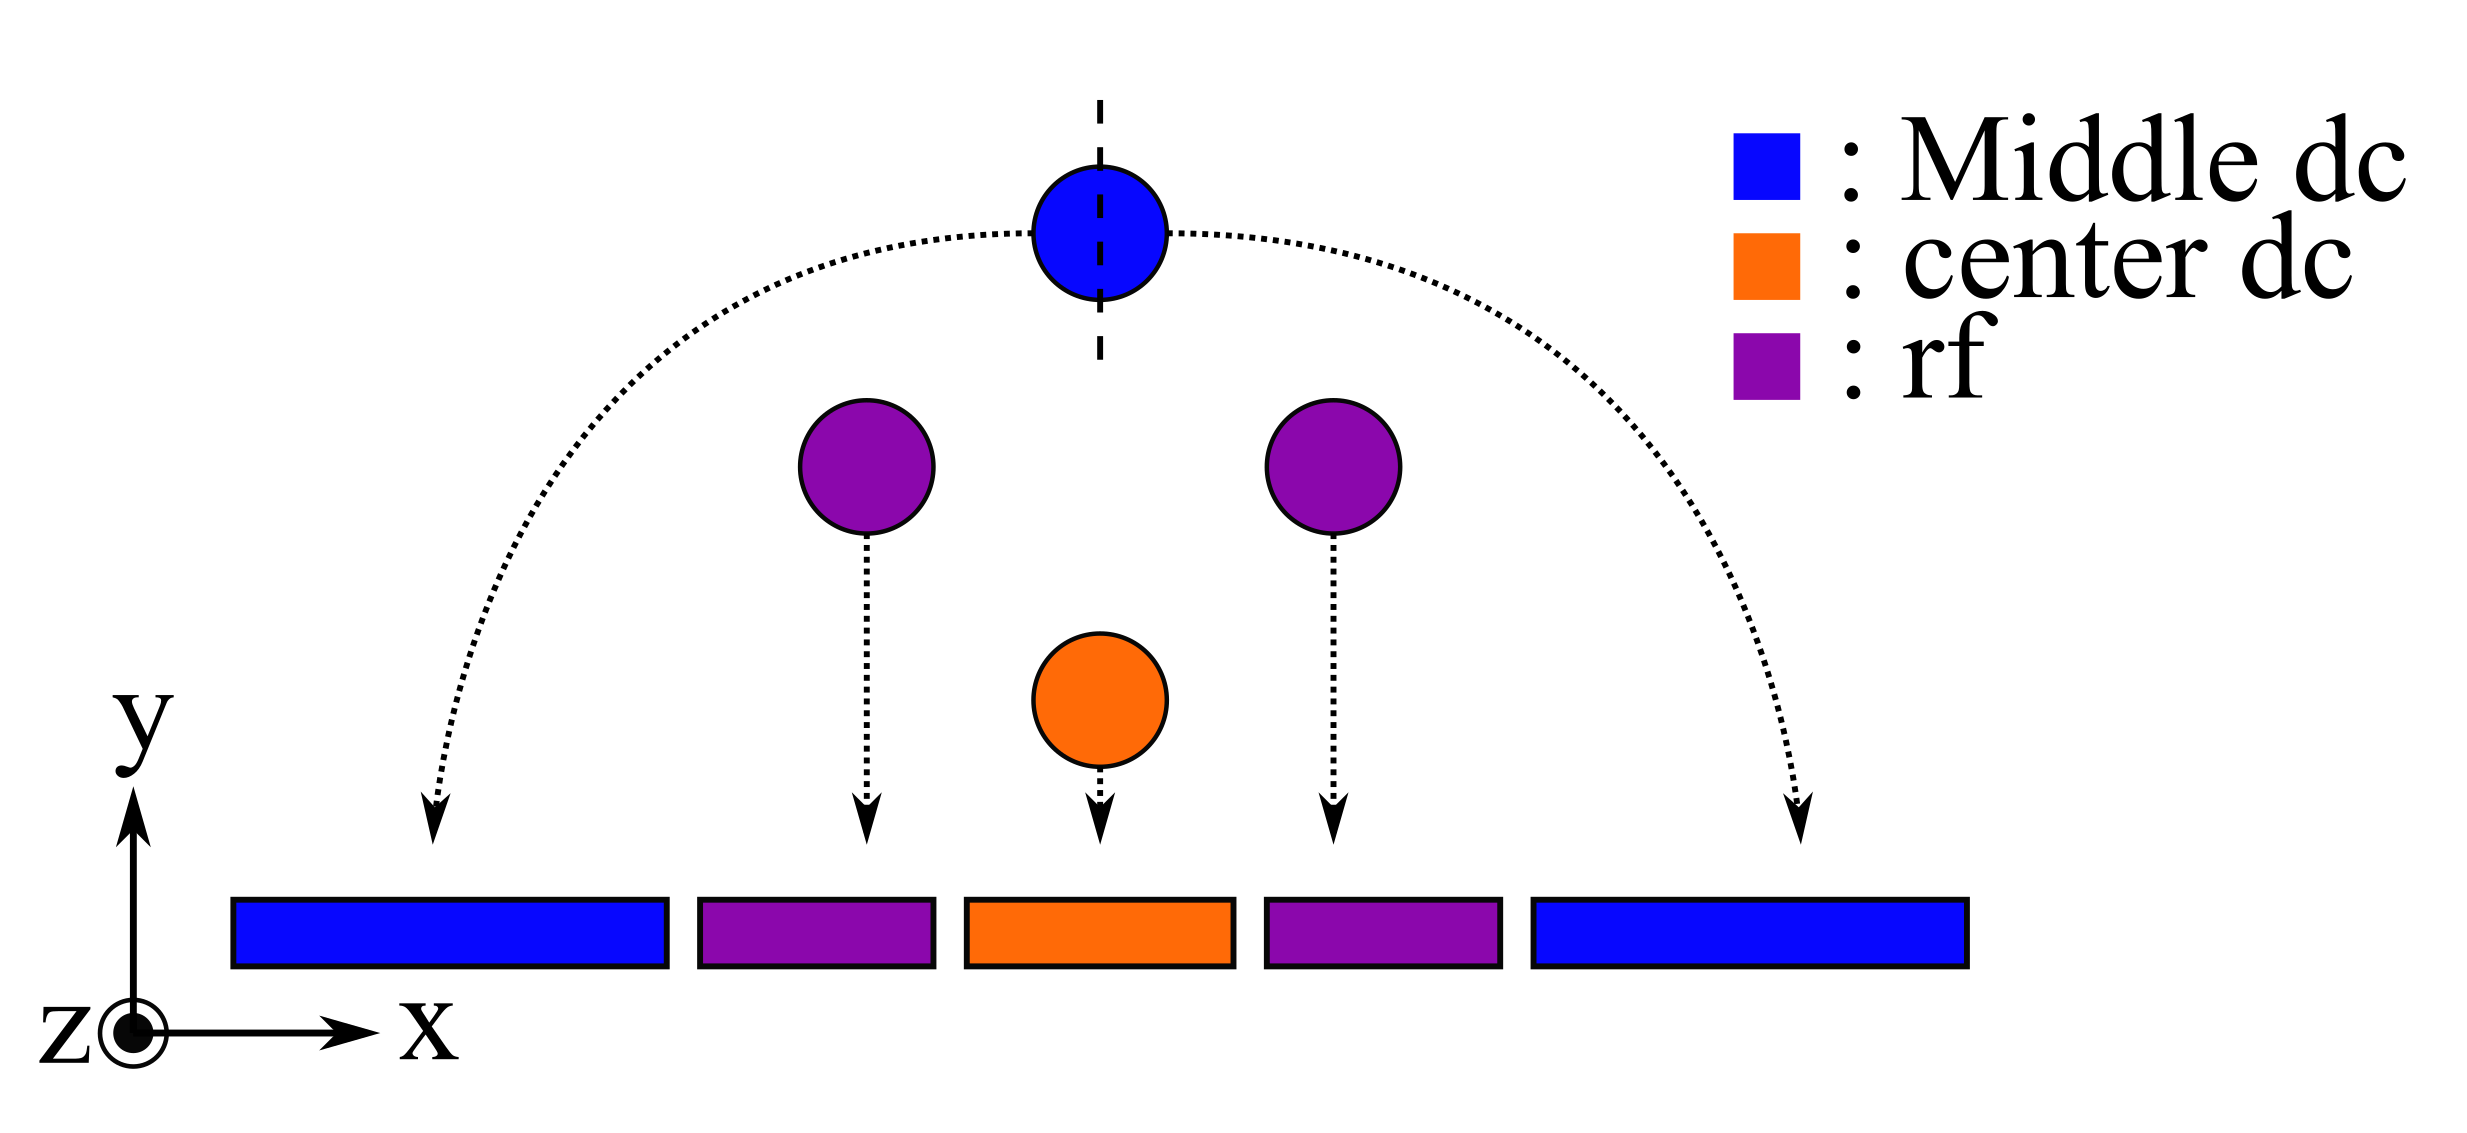
\includegraphics[width = 0.98\columnwidth]{./theory/figure/PaulTrap_3Dto2D_3DTrap.png}
			\end{center}
		\end{minipage}
		\begin{minipage}{0.48\linewidth}
			\begin{center}
			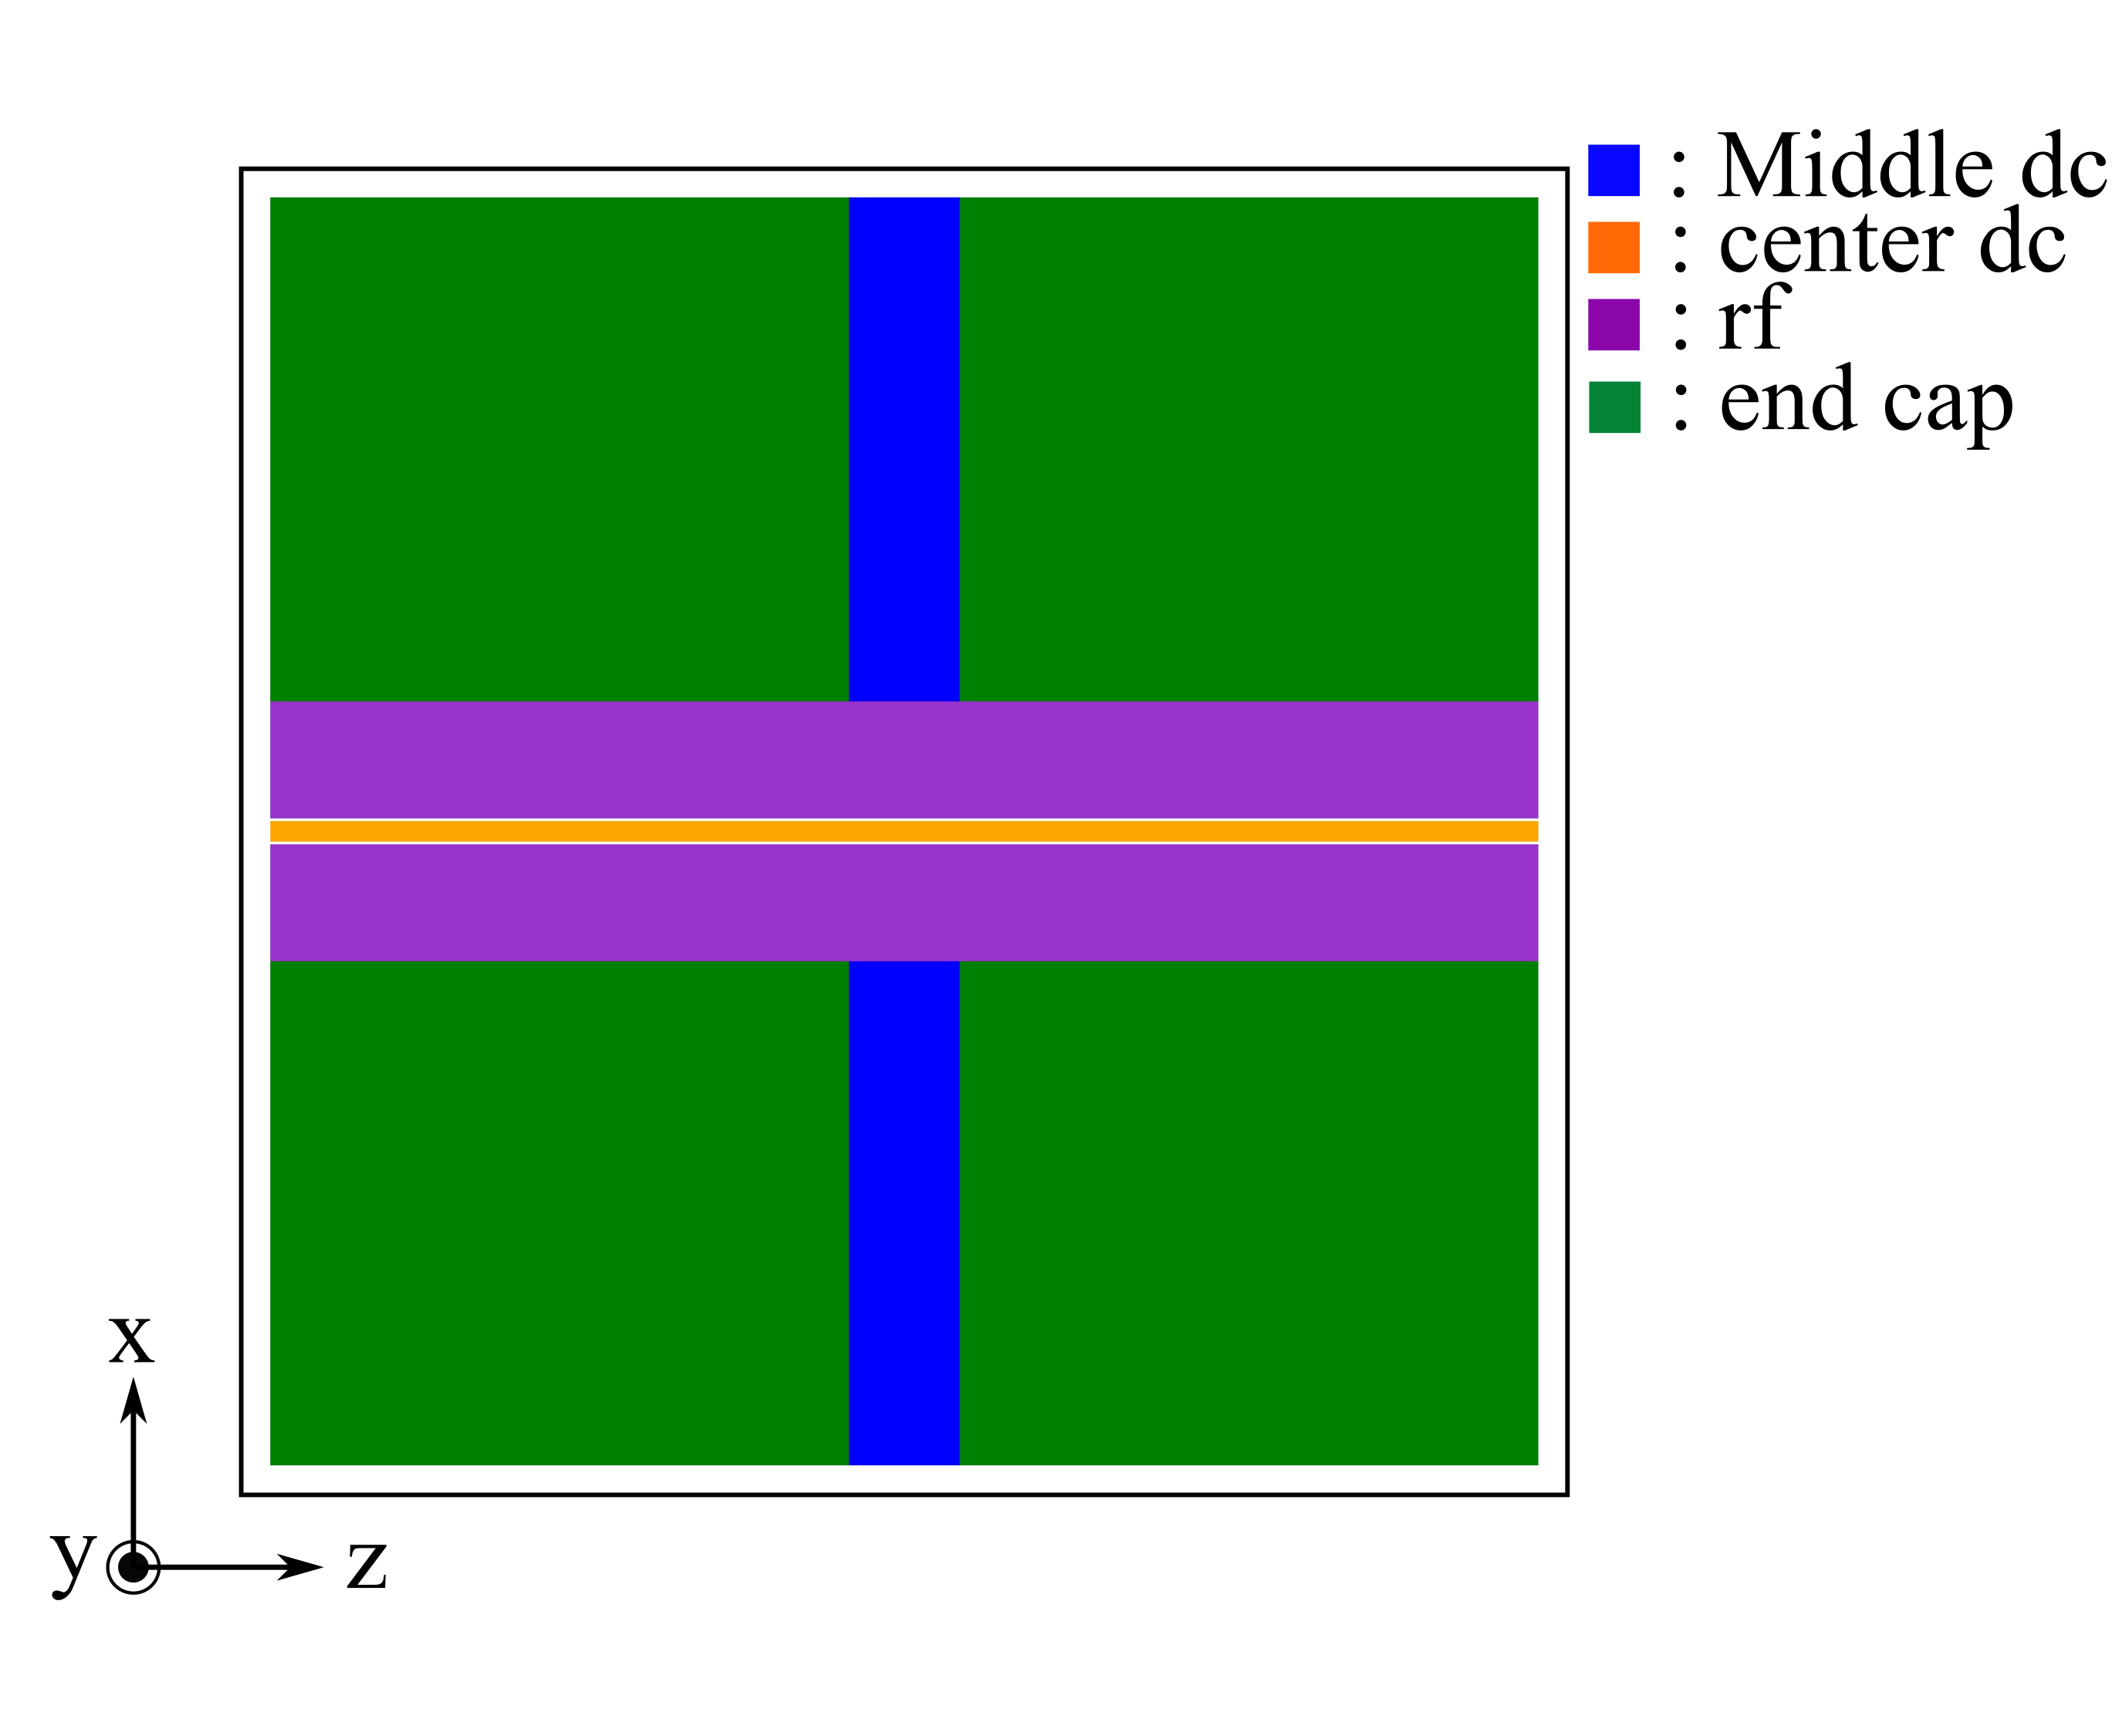
\includegraphics[width = 0.98\columnwidth]{./theory/figure/PaulTrap_3Dto2D_2DTrap.png}
			\end{center}
		\end{minipage}
	\end{center}
	\caption{立体的なパウルトラップとプレーナー型パウルトラップとの対応関係}
\end{figure}
\subsection{電極の仕様}
\begin{figure}[h]
	\begin{center}
		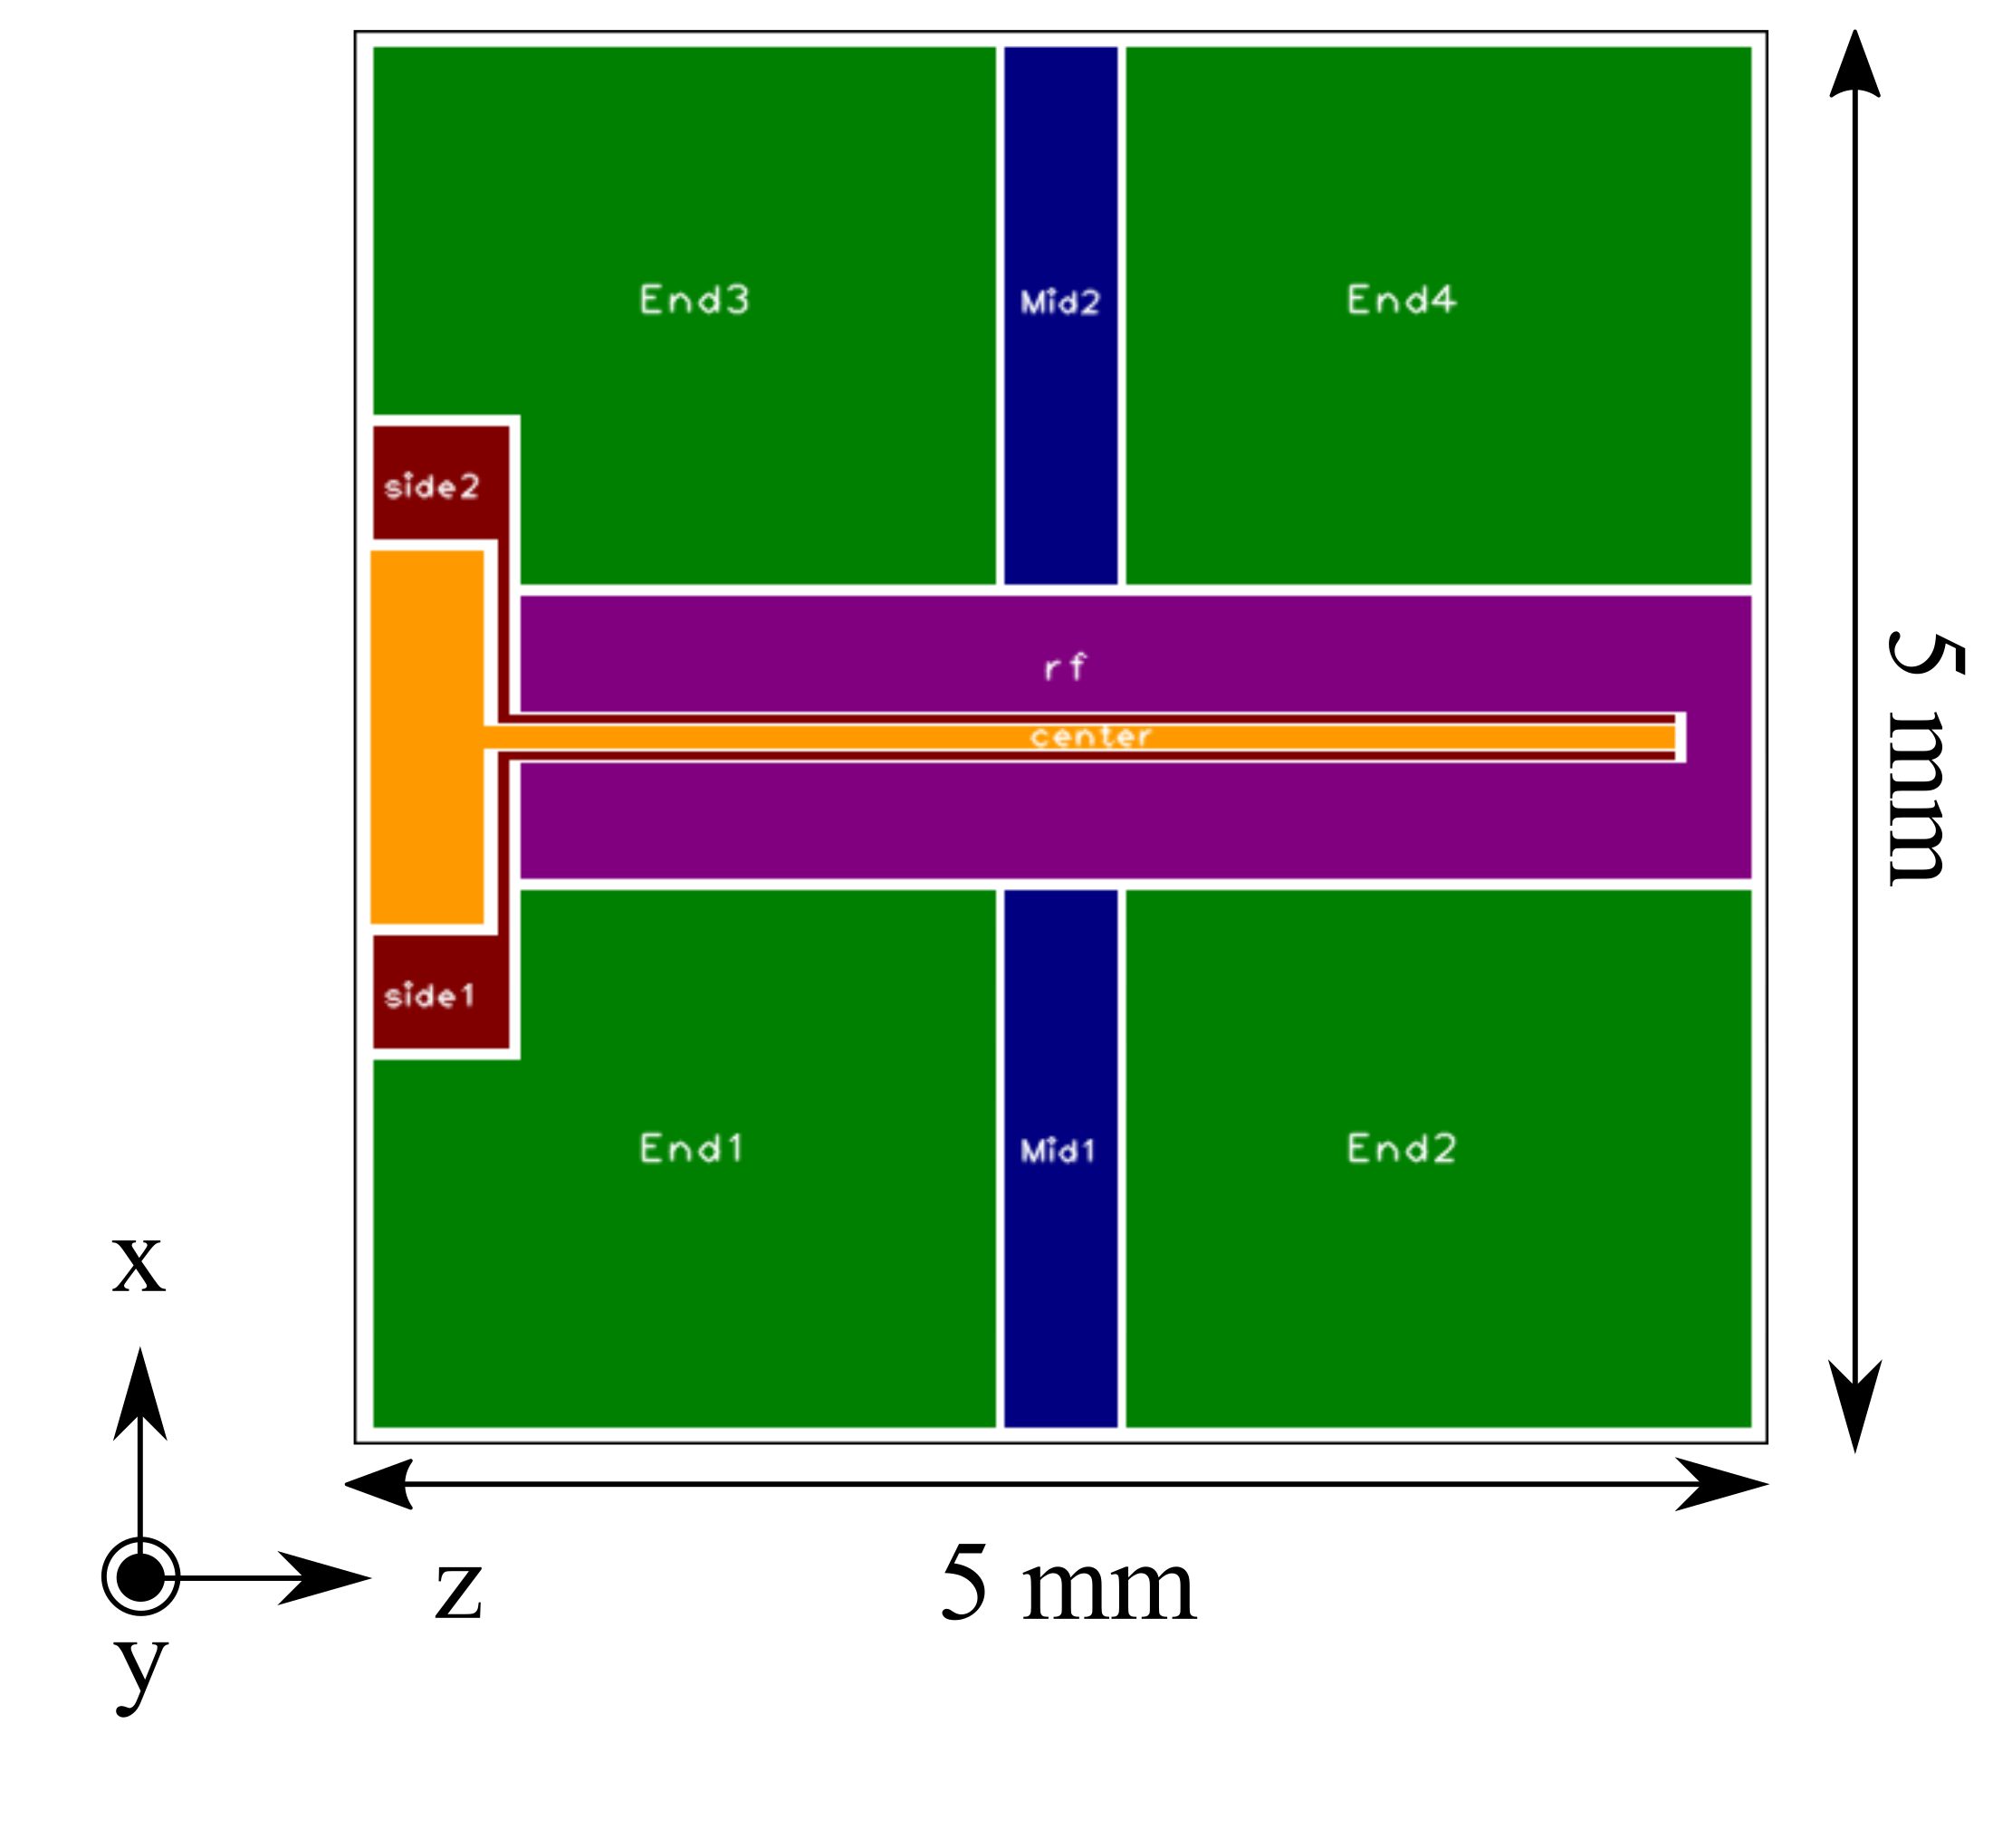
\includegraphics[width = 0.5\linewidth]{./theory/figure/named_electrode.png}
		\caption{本実験で使用するプレーナー型パウルトラップの電極モデル}
		\label{fig:Named_PlannerTrap}
	\end{center}
\end{figure}
以下では,プレーナー型パウルトラップのことを単にプレーナートラップと呼ぶ.
\subsection{矩形電極が作る静電ポテンシャル}
\begin{figure}[h]
	\begin{center}
		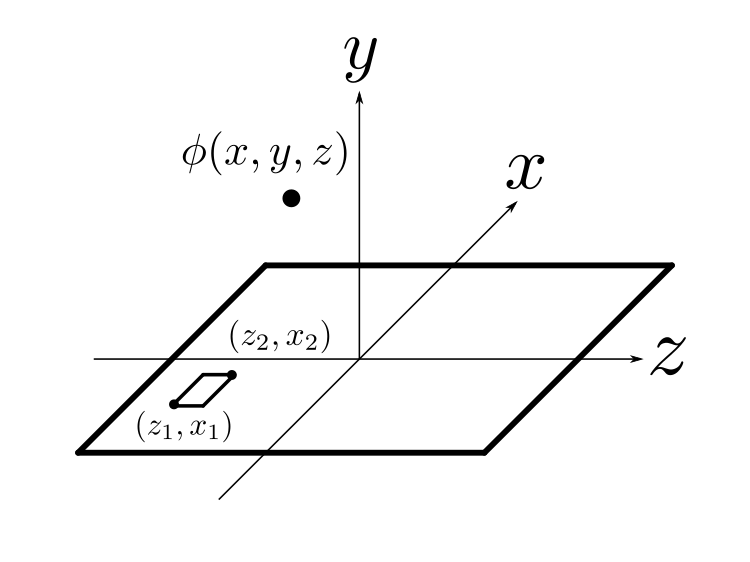
\includegraphics[width = 0.5\linewidth]{./theory/figure/Potential_of_rect-electrode.png}
		\caption{$(z_1,x_1),(z_2,x_2)$で指定される矩形が任意の点$(x,y,z)$に形成する静電ポテンシャル}
		\label{fig:Potential_from_rect-electrode}
	\end{center}
\end{figure}
\begin{align}\label{eq:rectangle_electrode}
	\phi(x,y,z) = \frac{V}{2\pi} \left\lbrace \arctan \left[ \frac{(x_2 - x)(z_2 - z)}{y\sqrt{y^2 + (x_2 - x)^2 + (z_2 - z)^2}}\right] - \arctan \left[ \frac{(x_1 - x)(z_2 - z)}{y\sqrt{y^2 + (x_1 - x)^2 + (z_2 - z)^2}} \right]  \right.  \notag \\ 
	\left. -\arctan \left[ \frac{(x_2 - x)(z_1 - z)}{y\sqrt{y^2 + (x_2 - x)^2 + (z_1 - z)^2}}\right] + \arctan \left[ \frac{(x_1 - x)(z_1 - z)}{y\sqrt{y^2 + (x_1 - x)^2 + (z_1 - z)^2}} \right]  \right\rbrace 
\end{align}
\section{レーザー冷却}

\section{画像処理によるイオン捕獲位置と電場の算出}
OpenCVとNumpyを使って画像処理を行うことでイオンの位置と,イオンの位置における電場の算出を行う.ここでは画像処理の方法について述べる.
\subsection{ヒストグラムの正規化}
カメラでイオンの蛍光を撮像する際に,カメラの集光時間やピントおよび照射するレーザーの波長や位置などによって得られるイオン捕獲画像の輝度値のヒストグラムは変化する.輝度値が0に近い画素が多ければ画像は全体として暗く,255に近い画素が多ければ画像は全体として明るくなる.\Fig{ionimage}に示すイオン捕獲画像を例にヒストグラムの偏りを\Fig{hist}に示す.
\begin{figure}[h]
	\begin{center}
	\begin{minipage}{0.3\linewidth}
		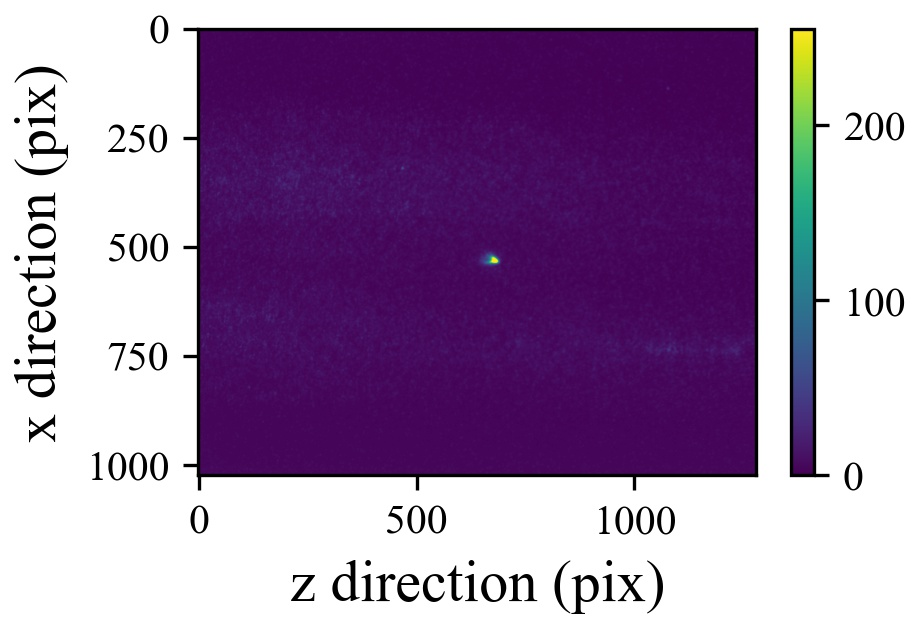
\includegraphics[width=0.98\columnwidth]{./theory/figure/5/image_0.jpg}
	\end{minipage}
	\begin{minipage}{0.3\linewidth}
		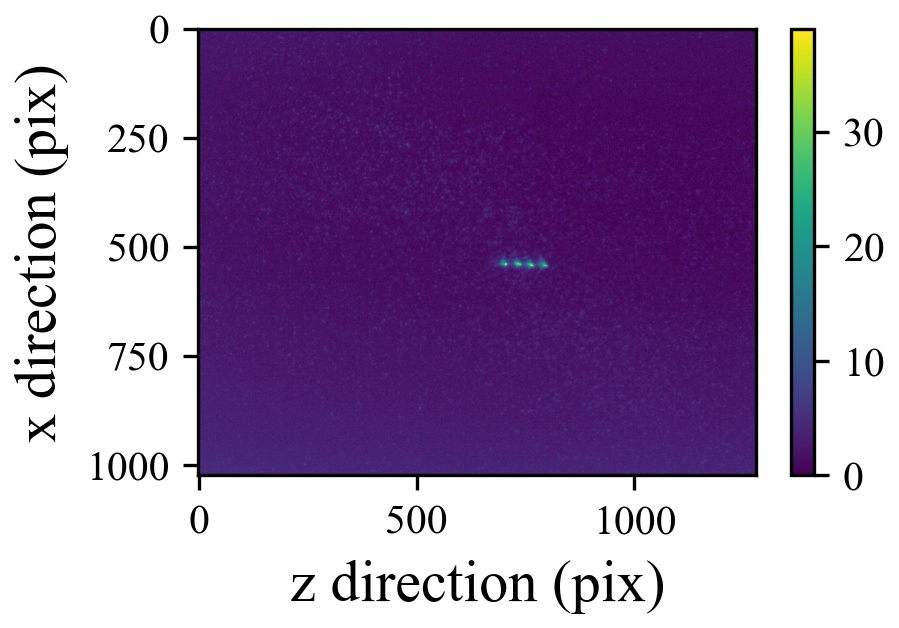
\includegraphics[width=0.98\columnwidth]{./theory/figure/5/image_1.jpg}
	\end{minipage}
	\begin{minipage}{0.3\linewidth}
		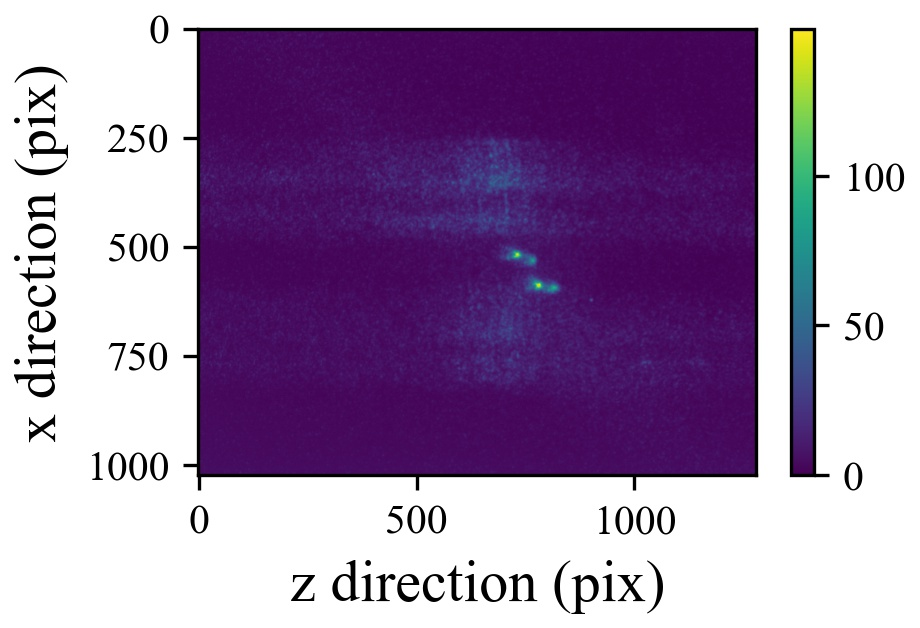
\includegraphics[width=0.98\columnwidth]{./theory/figure/5/image_2.jpg}
	\end{minipage}
	\end{center}
	\caption{集光系のピントおよびレーザー照射位置などが異なる場合のイオン捕獲画像}
	\label{fig:ionimage}
\end{figure}

\begin{figure}[h]
	\begin{center}
		\begin{minipage}{0.3\linewidth}
			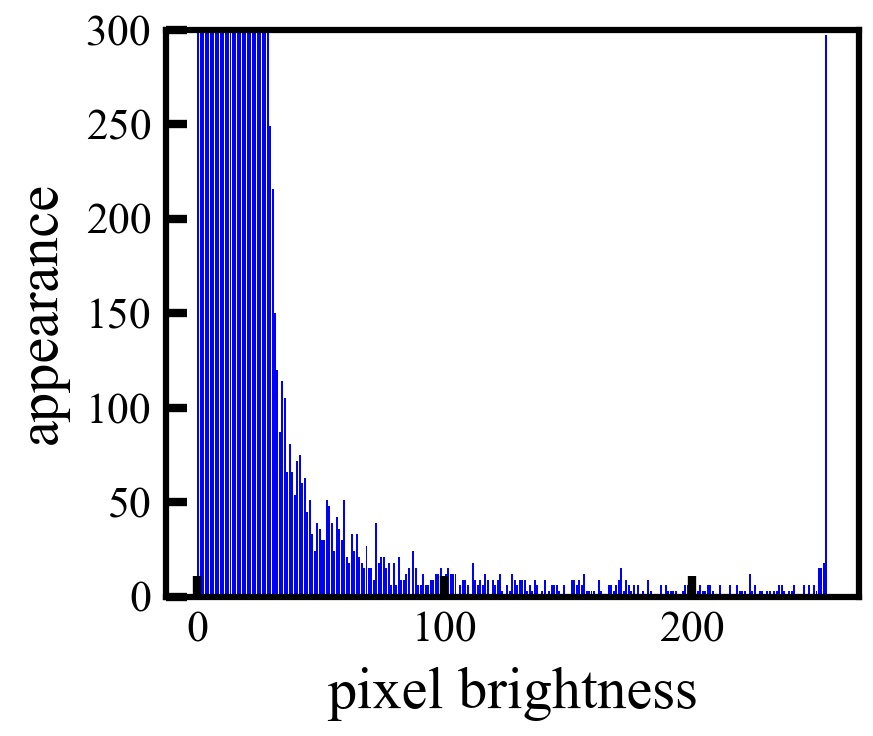
\includegraphics[width=0.98\columnwidth]{./theory/figure/5/hist_0.jpg}
		\end{minipage}
		\begin{minipage}{0.3\linewidth}
			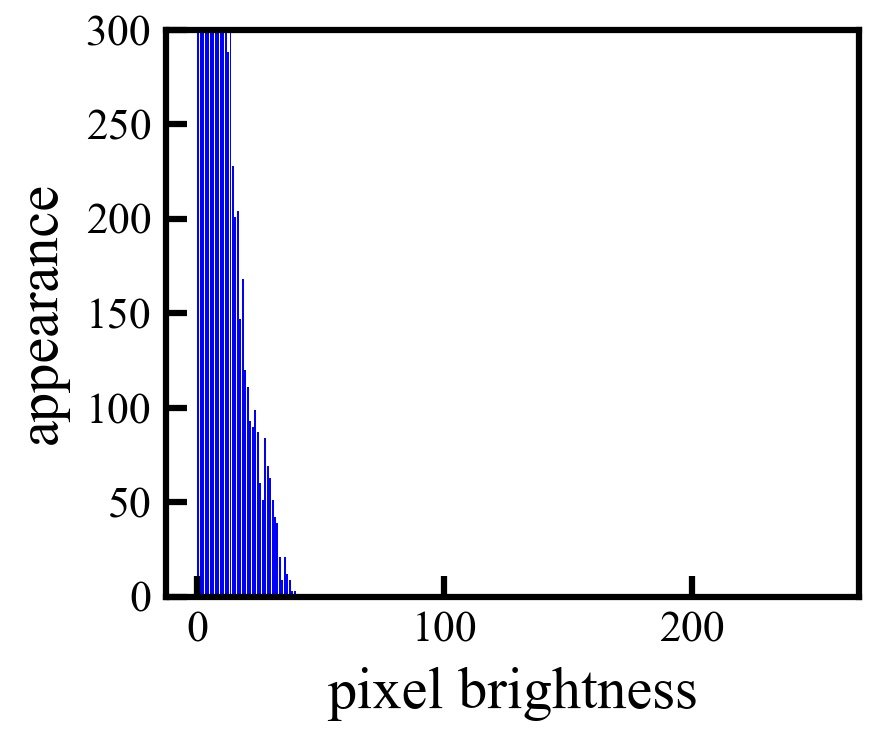
\includegraphics[width=0.98\columnwidth]{./theory/figure/5/hist_1.jpg}
		\end{minipage}
		\begin{minipage}{0.3\linewidth}
			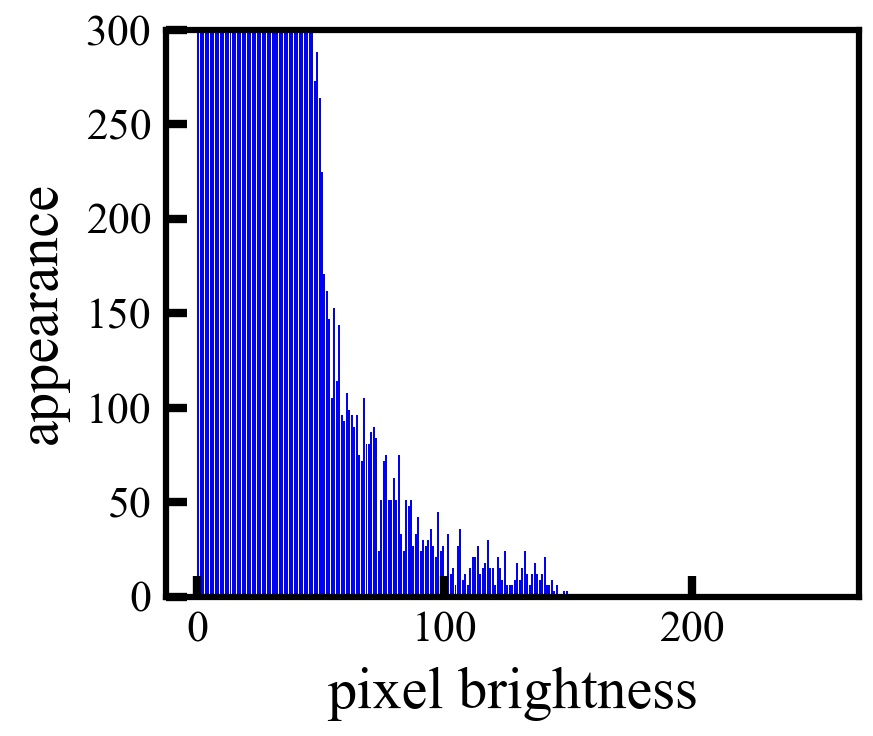
\includegraphics[width=0.98\columnwidth]{./theory/figure/5/hist_2.jpg}
		\end{minipage}
	\end{center}
	\caption{\Fig{ionimage}の各画像のピクセル輝度値のヒストグラム}
	\label{fig:hist}
\end{figure}

イオンの位置特定を行うに際し,二値化の処理のための閾値を定める.しかし,\Fig{hist}のように輝度値の偏りが各画像において異なっている場合,閾値を画像毎に変化させる必要がある.これを防ぐために濃度諧調変換と呼ばれるヒストグラムの正規化を行う.[c,d]の画素値を持つ画像を[a,b]のレンジに変換する式は次式で与えられる.

\large
\begin{align}\label{eq:GS_trans}
x_{\rm out} = 
\left\{ 
\begin{array}{ll}
	a & {\rm if} \ x_{\rm in} < c \\
	\frac{b-a}{d-c}(x_{\rm in}-c) + a & {\rm else \ if} \ c \leq x_{\rm in} < d \\
	b &{\rm else}
\end{array} \right.
\end{align}
\normalsize
ここでa,bは任意であり,cはある画像における輝度値の最小値,dは最大値とする.

\Fig{hist}に対して\Eq{GS_trans}を$a=0,b=255$として適用させると\Fig{norm_hist}となる.
\begin{figure}[h]
	\begin{center}
		\begin{minipage}{0.3\linewidth}
			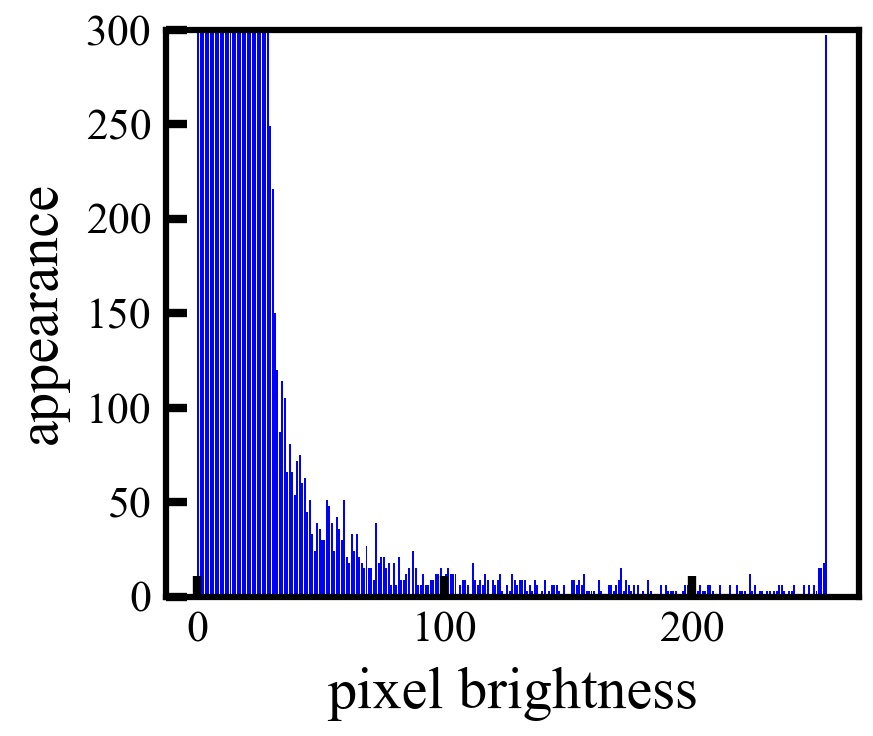
\includegraphics[width=0.98\columnwidth]{./theory/figure/5/norm_hist_0.jpg}
		\end{minipage}
		\begin{minipage}{0.3\linewidth}
			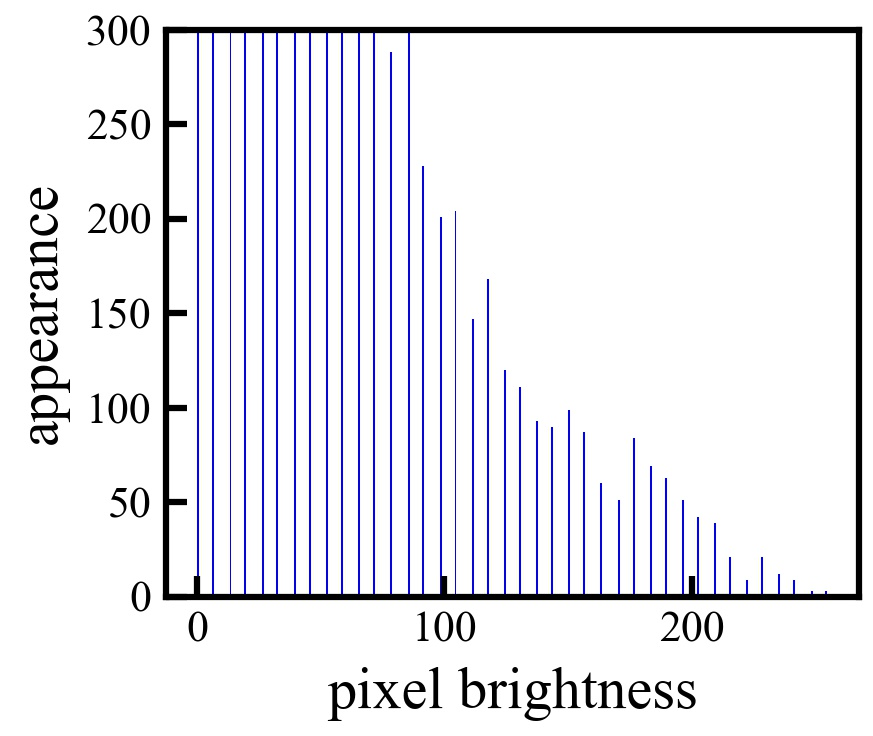
\includegraphics[width=0.98\columnwidth]{./theory/figure/5/norm_hist_1.jpg}
		\end{minipage}
		\begin{minipage}{0.3\linewidth}
			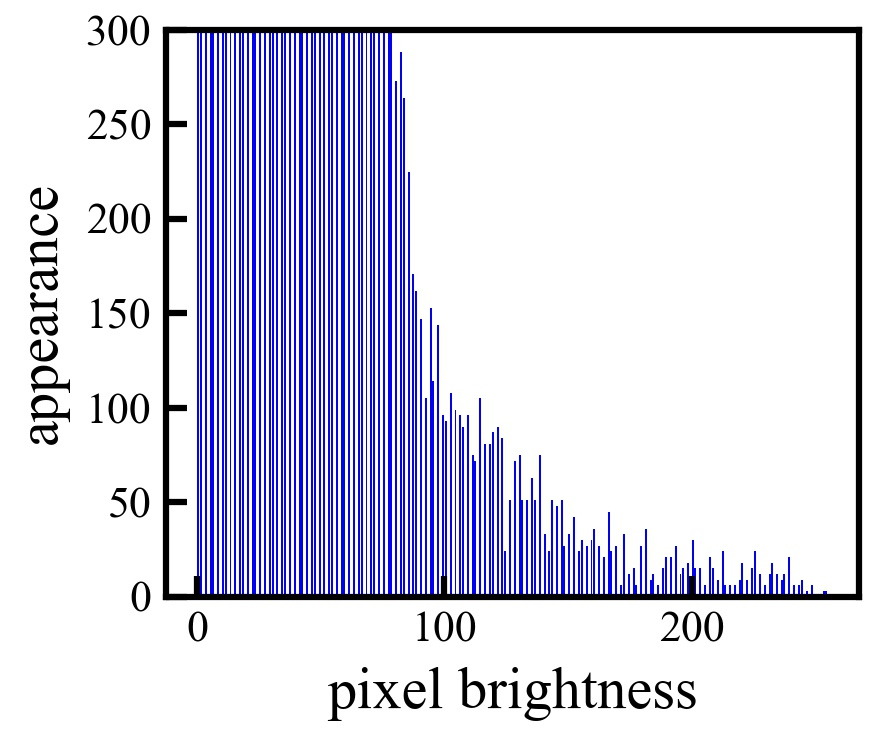
\includegraphics[width=0.98\columnwidth]{./theory/figure/5/norm_hist_2.jpg}
		\end{minipage}
	\end{center}
	\caption{\Fig{ionimage}の各画像のピクセル輝度値を正規化したときのヒストグラム}
	\label{fig:norm_hist}
\end{figure}

\subsection{二値化}
二値化とは,画像を特定の値を閾値として黒(=0)と白(=255)の2値で表現する方法である.二値化は次式で表される式を用いて変換される.
\large
\begin{align}\label{eq:binary_trans}
	x_{\rm out} = 
	\left\{ 
	\begin{array}{ll}
		0 & {\rm if} \ x_{\rm in} < {\rm threshold} \\
		255 & {\rm otherwise}
	\end{array} \right.
\end{align}
\normalsize
\Fig{thre_norm_hist}に\Eq{binary_trans}を${\rm threshold} = 128$として二値化を行ったときのヒストグラムを\Fig{binary_hist}に示す.
\begin{figure}[h]
	\begin{center}
		\begin{minipage}{0.3\linewidth}
			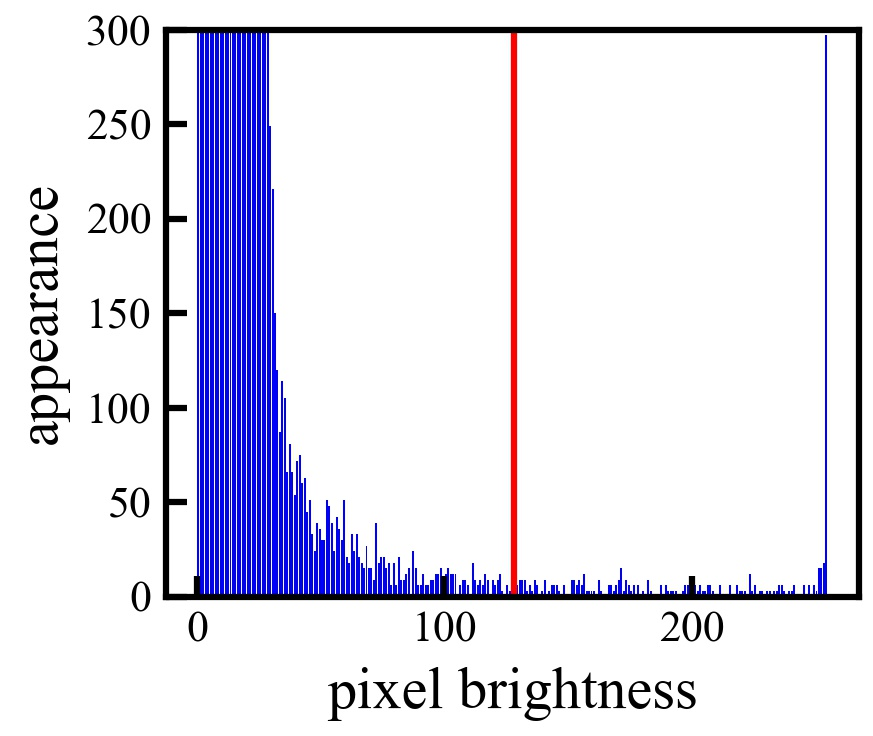
\includegraphics[width=0.98\columnwidth]{./theory/figure/5/thre_norm_hist_0.jpg}
		\end{minipage}
		\begin{minipage}{0.3\linewidth}
			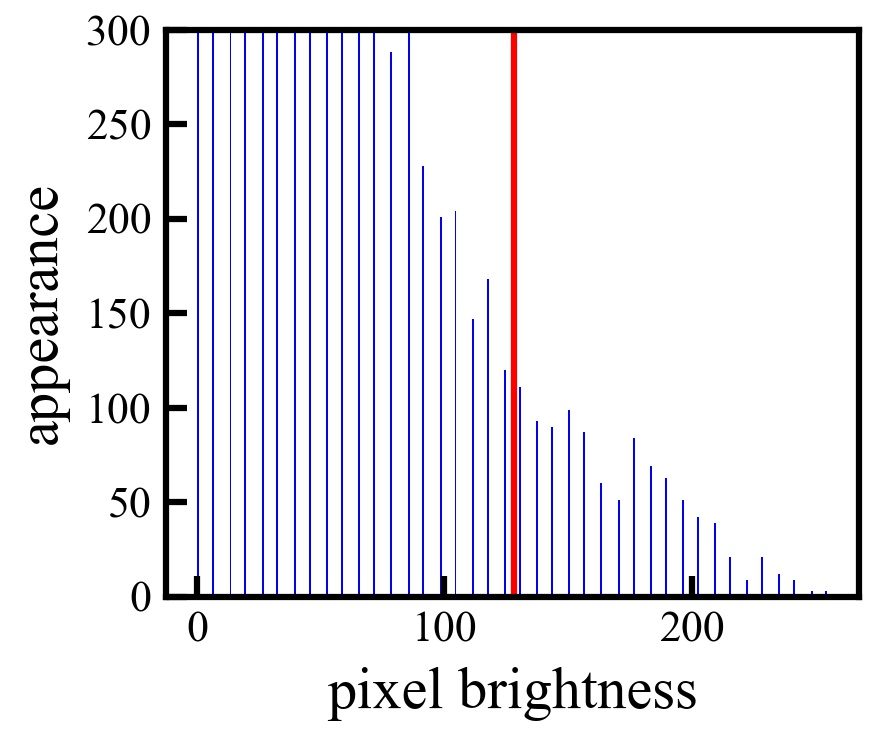
\includegraphics[width=0.98\columnwidth]{./theory/figure/5/thre_norm_hist_1.jpg}
		\end{minipage}
		\begin{minipage}{0.3\linewidth}
			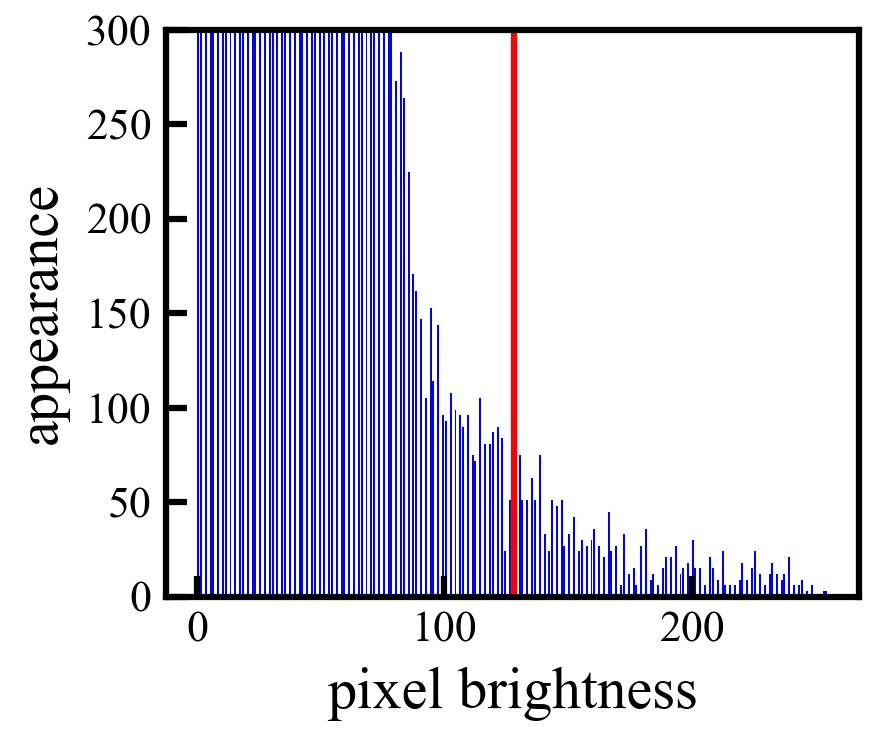
\includegraphics[width=0.98\columnwidth]{./theory/figure/5/thre_norm_hist_2.jpg}
		\end{minipage}
	\end{center}
	\caption{正規化されたヒストグラムにおける閾値(threshold = 128)の設定}
	\label{fig:thre_norm_hist}
\end{figure}

\begin{figure}[h]
	\begin{center}
		\begin{minipage}{0.3\linewidth}
			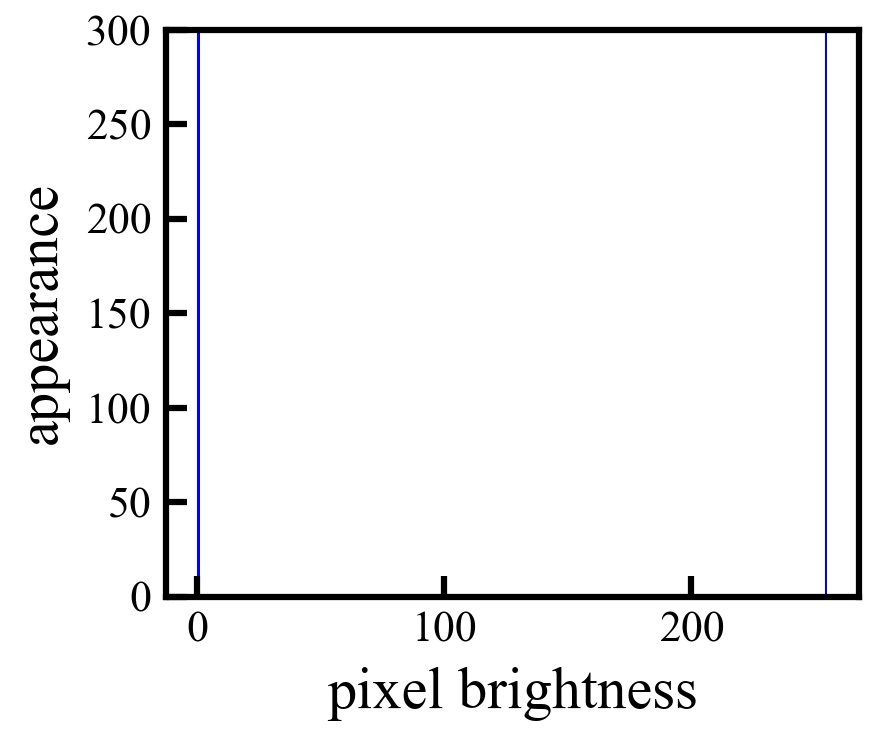
\includegraphics[width=0.98\columnwidth]{./theory/figure/5/binary_0.jpg}
		\end{minipage}
		\begin{minipage}{0.3\linewidth}
			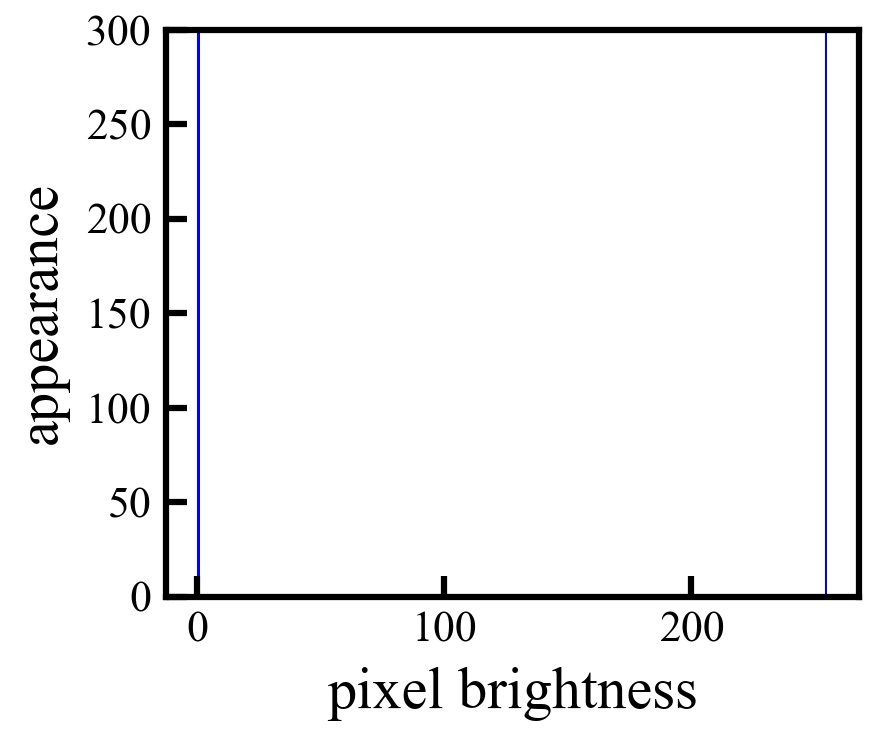
\includegraphics[width=0.98\columnwidth]{./theory/figure/5/binary_1.jpg}
		\end{minipage}
		\begin{minipage}{0.3\linewidth}
			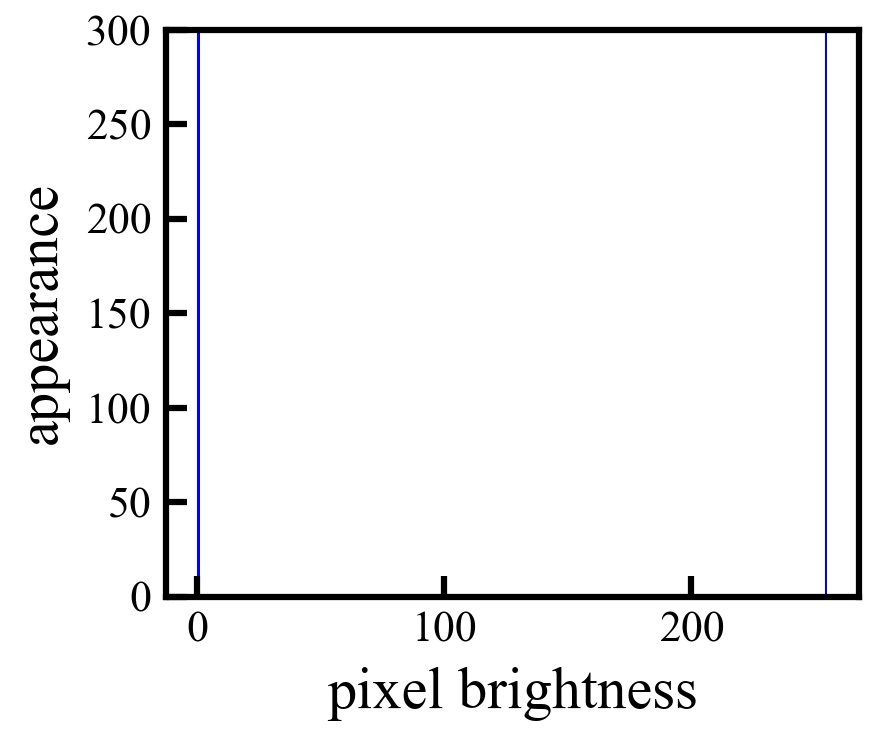
\includegraphics[width=0.98\columnwidth]{./theory/figure/5/binary_2.jpg}
		\end{minipage}
	\end{center}
	\caption{\Fig{thre_norm_hist}に対して,二値化(0,255)の処理を行った後のヒストグラム}
	\label{fig:binary_hist}
\end{figure}

ヒストグラムの正規化を行ったことで,カメラのピントや集光時間およびレーザーの波長や位置の影響を受ける画像の輝度値の二値化が固定の閾値で行うことができる.

\subsection{OpenCVを用いたイオンの検出}
二値化されたイオン捕獲画像において輝度値が255である範囲の面積を求め,ある値以上の面積を持つ範囲をイオンとして計上する.イオンと判定された範囲に対して最小外接円を近似しその中心値をイオンの位置として特定する.

\subsection{電場の算出方法}
イオンの位置を用いて,イオンにかかる電場の算出が可能である.N個のイオンが一列に並んでいるとき,i番目のイオンの座標$z_{i}$における電場$\bm{E}(z_{i})$を求める.イオンが捕獲されている状態では,プレーナートラップが形成する電場から受ける力と他のイオンから受けるクーロン相互作用による力とがつりあっている.したがって,次式が成り立つ.
\large
\begin{align}\label{eq:equi_string}
e\bm{E}(z_i) + \frac{e^2}{4\pi \varepsilon_0} \sum^N_{i=0,i\neq j} \frac{z_i - z_j}{|z_i - z_j|^3} = 0.
\end{align}
\normalsize
ここで,$e$は素電荷,$\varepsilon_0$は真空の誘電率を示す.
イオンが二列に並ぶ場合にも,\Eq{equi_string}と同様に平衡の式を満たす.i番目のイオンの位置が($z_i,x_i$)で指定されるとき,
\large
\begin{align}\label{eq:equi_array}
e\bm{E}(z_i,x_i) + \frac{e^2}{4\pi \varepsilon_0}\sum^N_{i=1,i\neq j}\frac{1}{|\bm{r}_{ij}|^2}\frac{\bm{r}_{ij}}{|\bm{r}_{ij}|} = 0,
\end{align}
\normalsize
と書くことができる.ここで,
\large
\begin{align}
\bm{r}_{ij} &= (z_i - z_j)\hat{z} + (x_i - x_j)\hat{x} \notag \\
|\bm{r}_{ij}| &= \sqrt{(z_i - z_j)^2 + (x_i - x_j)^2} \notag 
\end{align}
\normalsize
であり,$\hat{z},\hat{x}$は各軸における単位ベクトルである.また,$\hat{r}_{ij} \equiv \bm{r}_{ij}/|\bm{r}_{ij}|$とすれば,\Eq{equi_array}は,
\large
\begin{align}\label{eq:equi_array_2}
e\bm{E}(z_i,x_i) = \frac{e^2}{4\pi \varepsilon_0}\sum^N_{i=1,i\neq j} \frac{1}{|\bm{r}_{ij}|^2}\hat{r}_{ij} = 0
\end{align}
\normalsize
とまとめられる.二列配列のイオン捕獲位置における電場を導出する際には,\Eq{equi_array_2}を各軸に沿った成分毎に計算を行う.したがって,各成分に分けて書くと,
\large
\begin{align}
eE_z(z_i,x_i) + \frac{e^2}{4\pi \varepsilon_0} \sum^N_{i=1,i \neq j}\frac{z_i - z_j}{|\bm{r}_{ij}|^3} = 0 , \\
eE_x(z_i,x_i) + \frac{e^2}{4\pi \varepsilon_0} \sum^N_{i=1,i \neq j}\frac{x_i - x_j}{|\bm{r}_{ij}|^3} = 0 .
\end{align}
\normalsize
これを解くことで,
\large
\begin{align}
\bm{E}(z,x) = E_z(z,x)\hat{z} + E_x(z,x)\hat{x}
\end{align}
\normalsize
の関係から,イオン捕獲位置における電場の算出を行う.電場の大きさと,z軸からの偏角$\theta$は,
\large
\begin{align}
|\bm{E}(z_i,x_i)| &= \sqrt{E_z^2(z_i,x_i) + E_x^2(z_i,x_i)}, \\
\theta &= \tan^{-1} \left(\frac{E_x(z_i,x_i)}{E_z(z_i,x_i)} \right) .
\end{align}
\normalsize

\section{イオンの平衡位置}
	% -- 実験装置 -- %
	\section{実験のセットアップ}

イオントラップに使用するレーザーのビーム径とその強度をスリット走査型光ビームプロファイラ(THORLABS,BP209-VIS/M)とデジタルパワー\&エネルギーメータ(THORLABS,PM100D)およびフォトダイオードパワーセンサー(THORLABS,S120C)を用いて計測を行った.
まず,各レーザーの強度を\Tb{AllLaserPower}に示す.

\begin{table}[h]
	\begin{center}
		\caption{各レーザーのパワー一覧表}
		\label{tab:AllLaserPower}
		\begin{tabular}{c|cccc} \hline \hline
			レーザーの波長 (nm)&375&397&423&866 \\ \hline
			パワー ($\mu$W)&4.1&17.4&28.4&700 \\ \hline
		\end{tabular}
	\end{center}
\end{table}

次に,ビーム径の計測結果を\Fig{AllLaserBeamProfile}に示す.

\begin{figure}[h]
	\begin{center}
	\begin{minipage}{0.48\linewidth}
		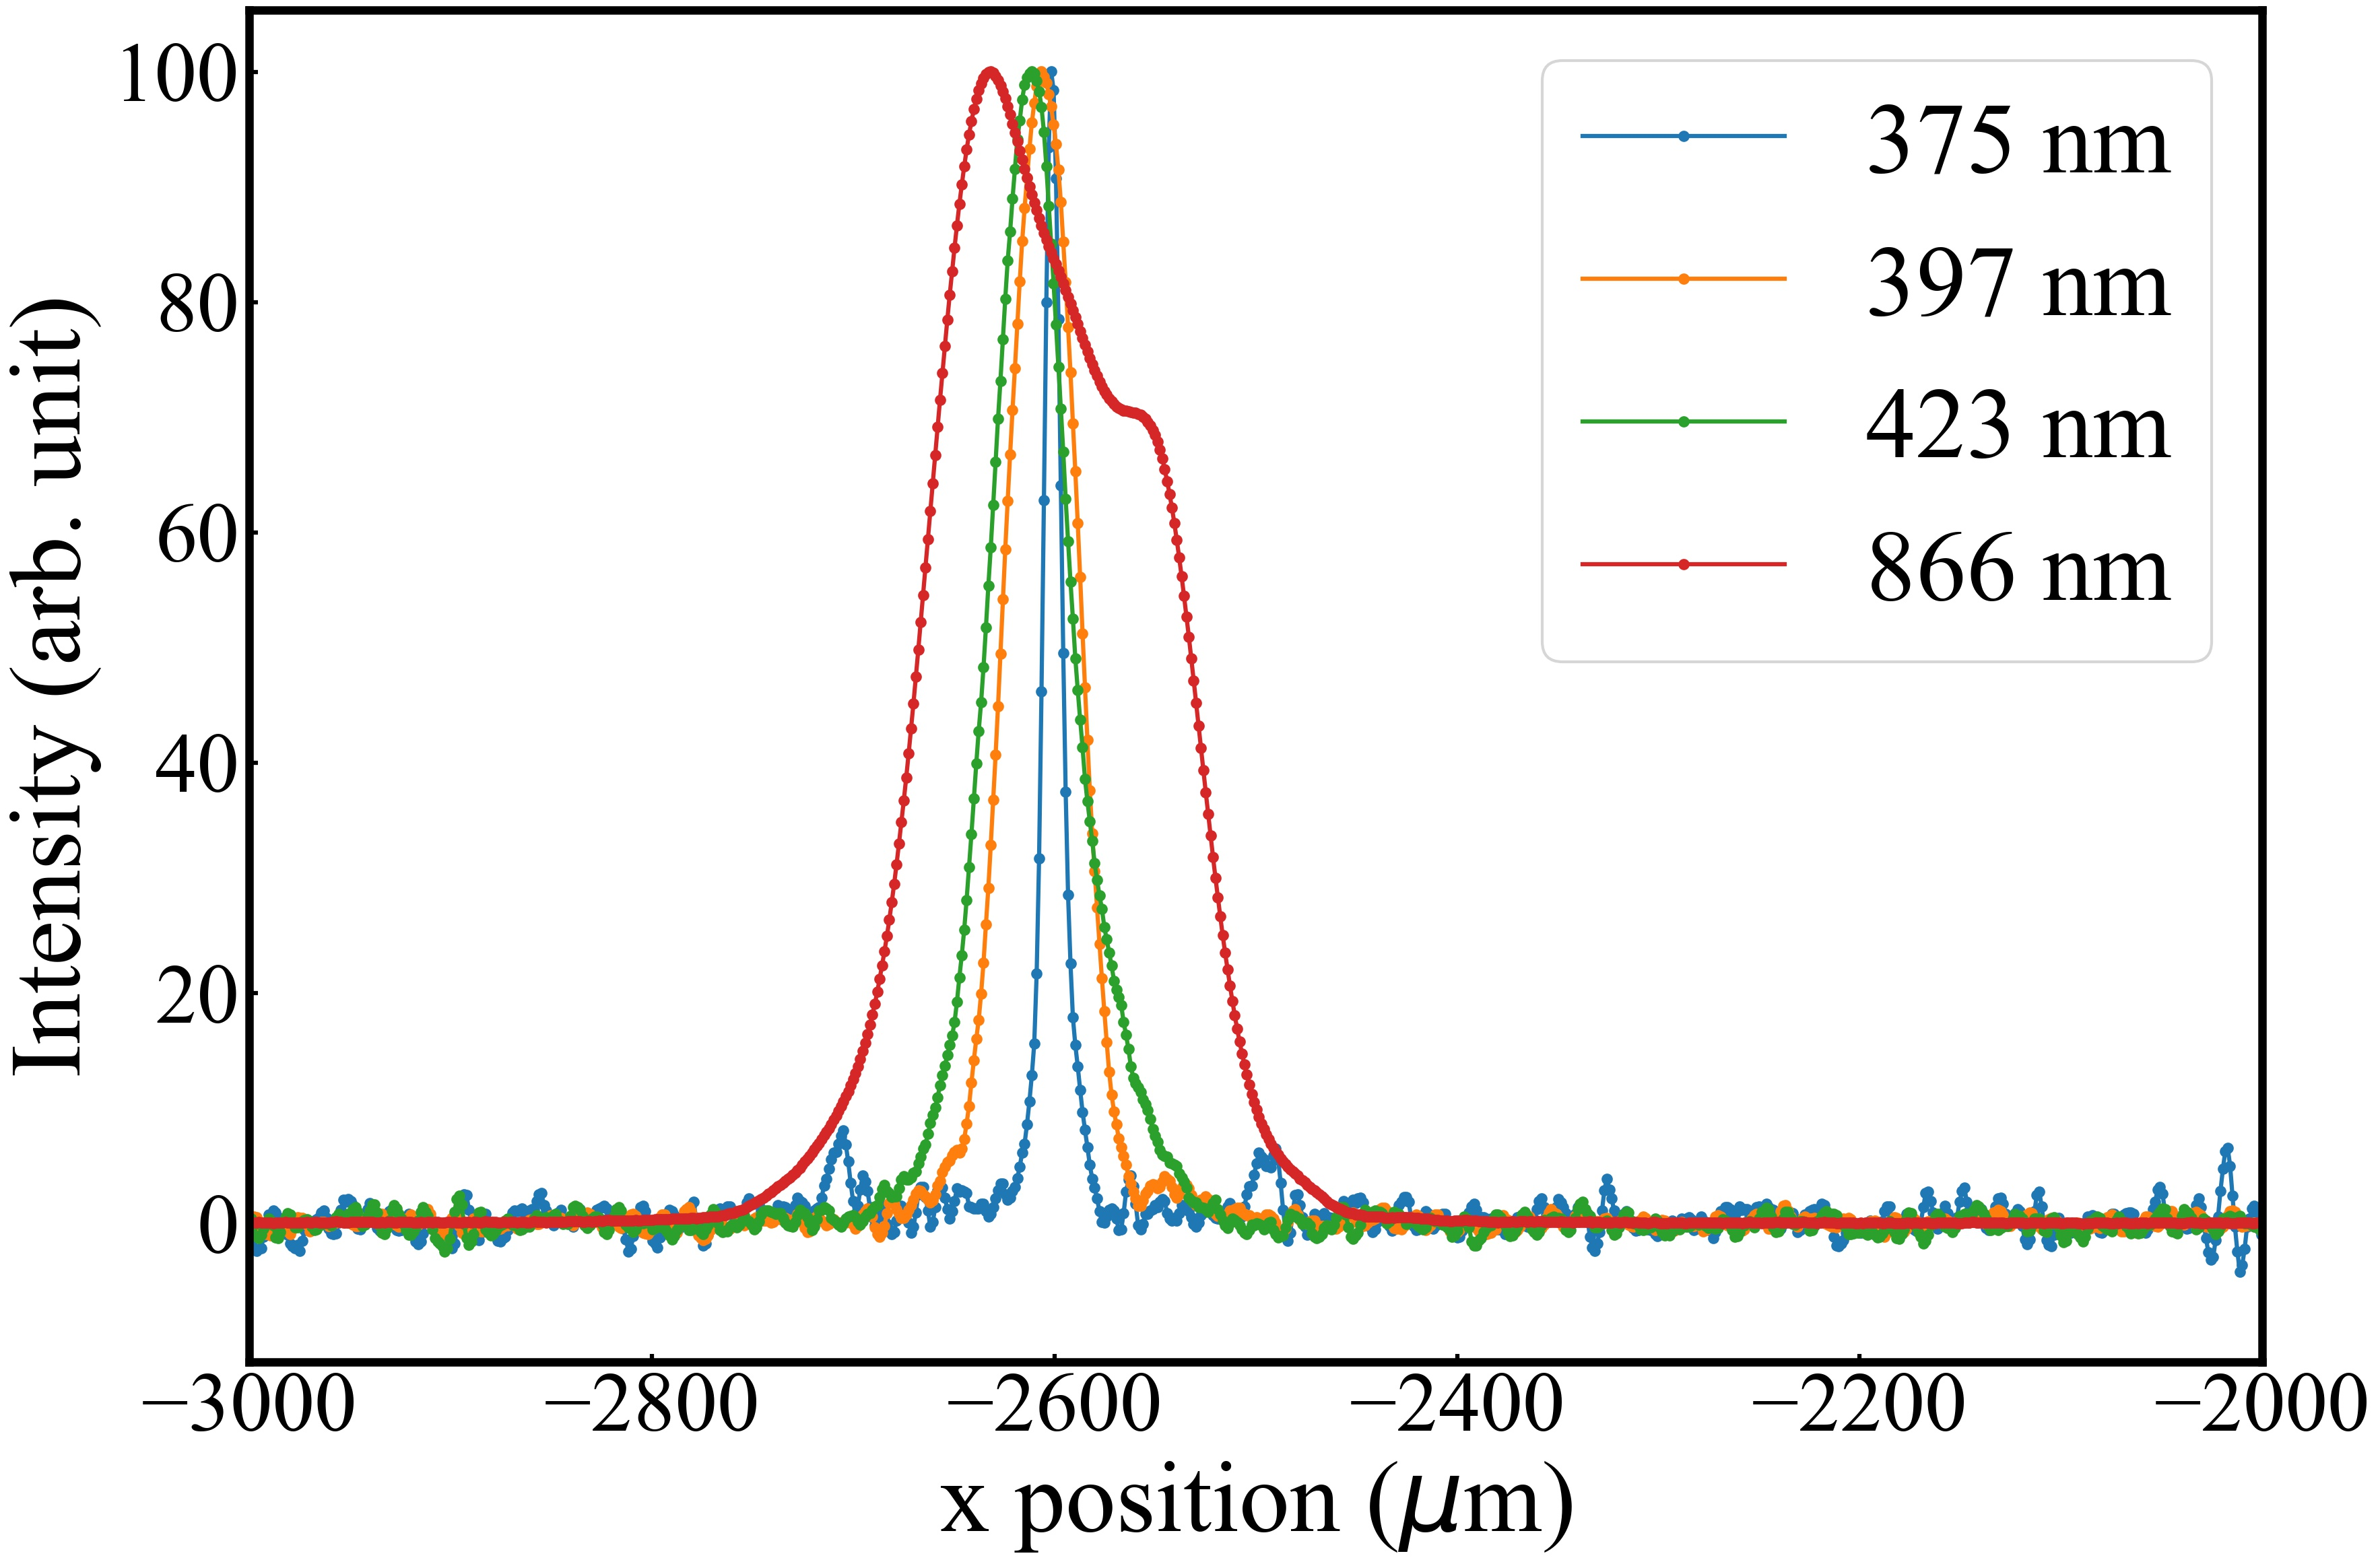
\includegraphics[width = 0.98\columnwidth]{./experimental_setup/figure/AllLaserXpos.jpg}
	\end{minipage}
	\begin{minipage}{0.48\linewidth}
		\begin{center}
		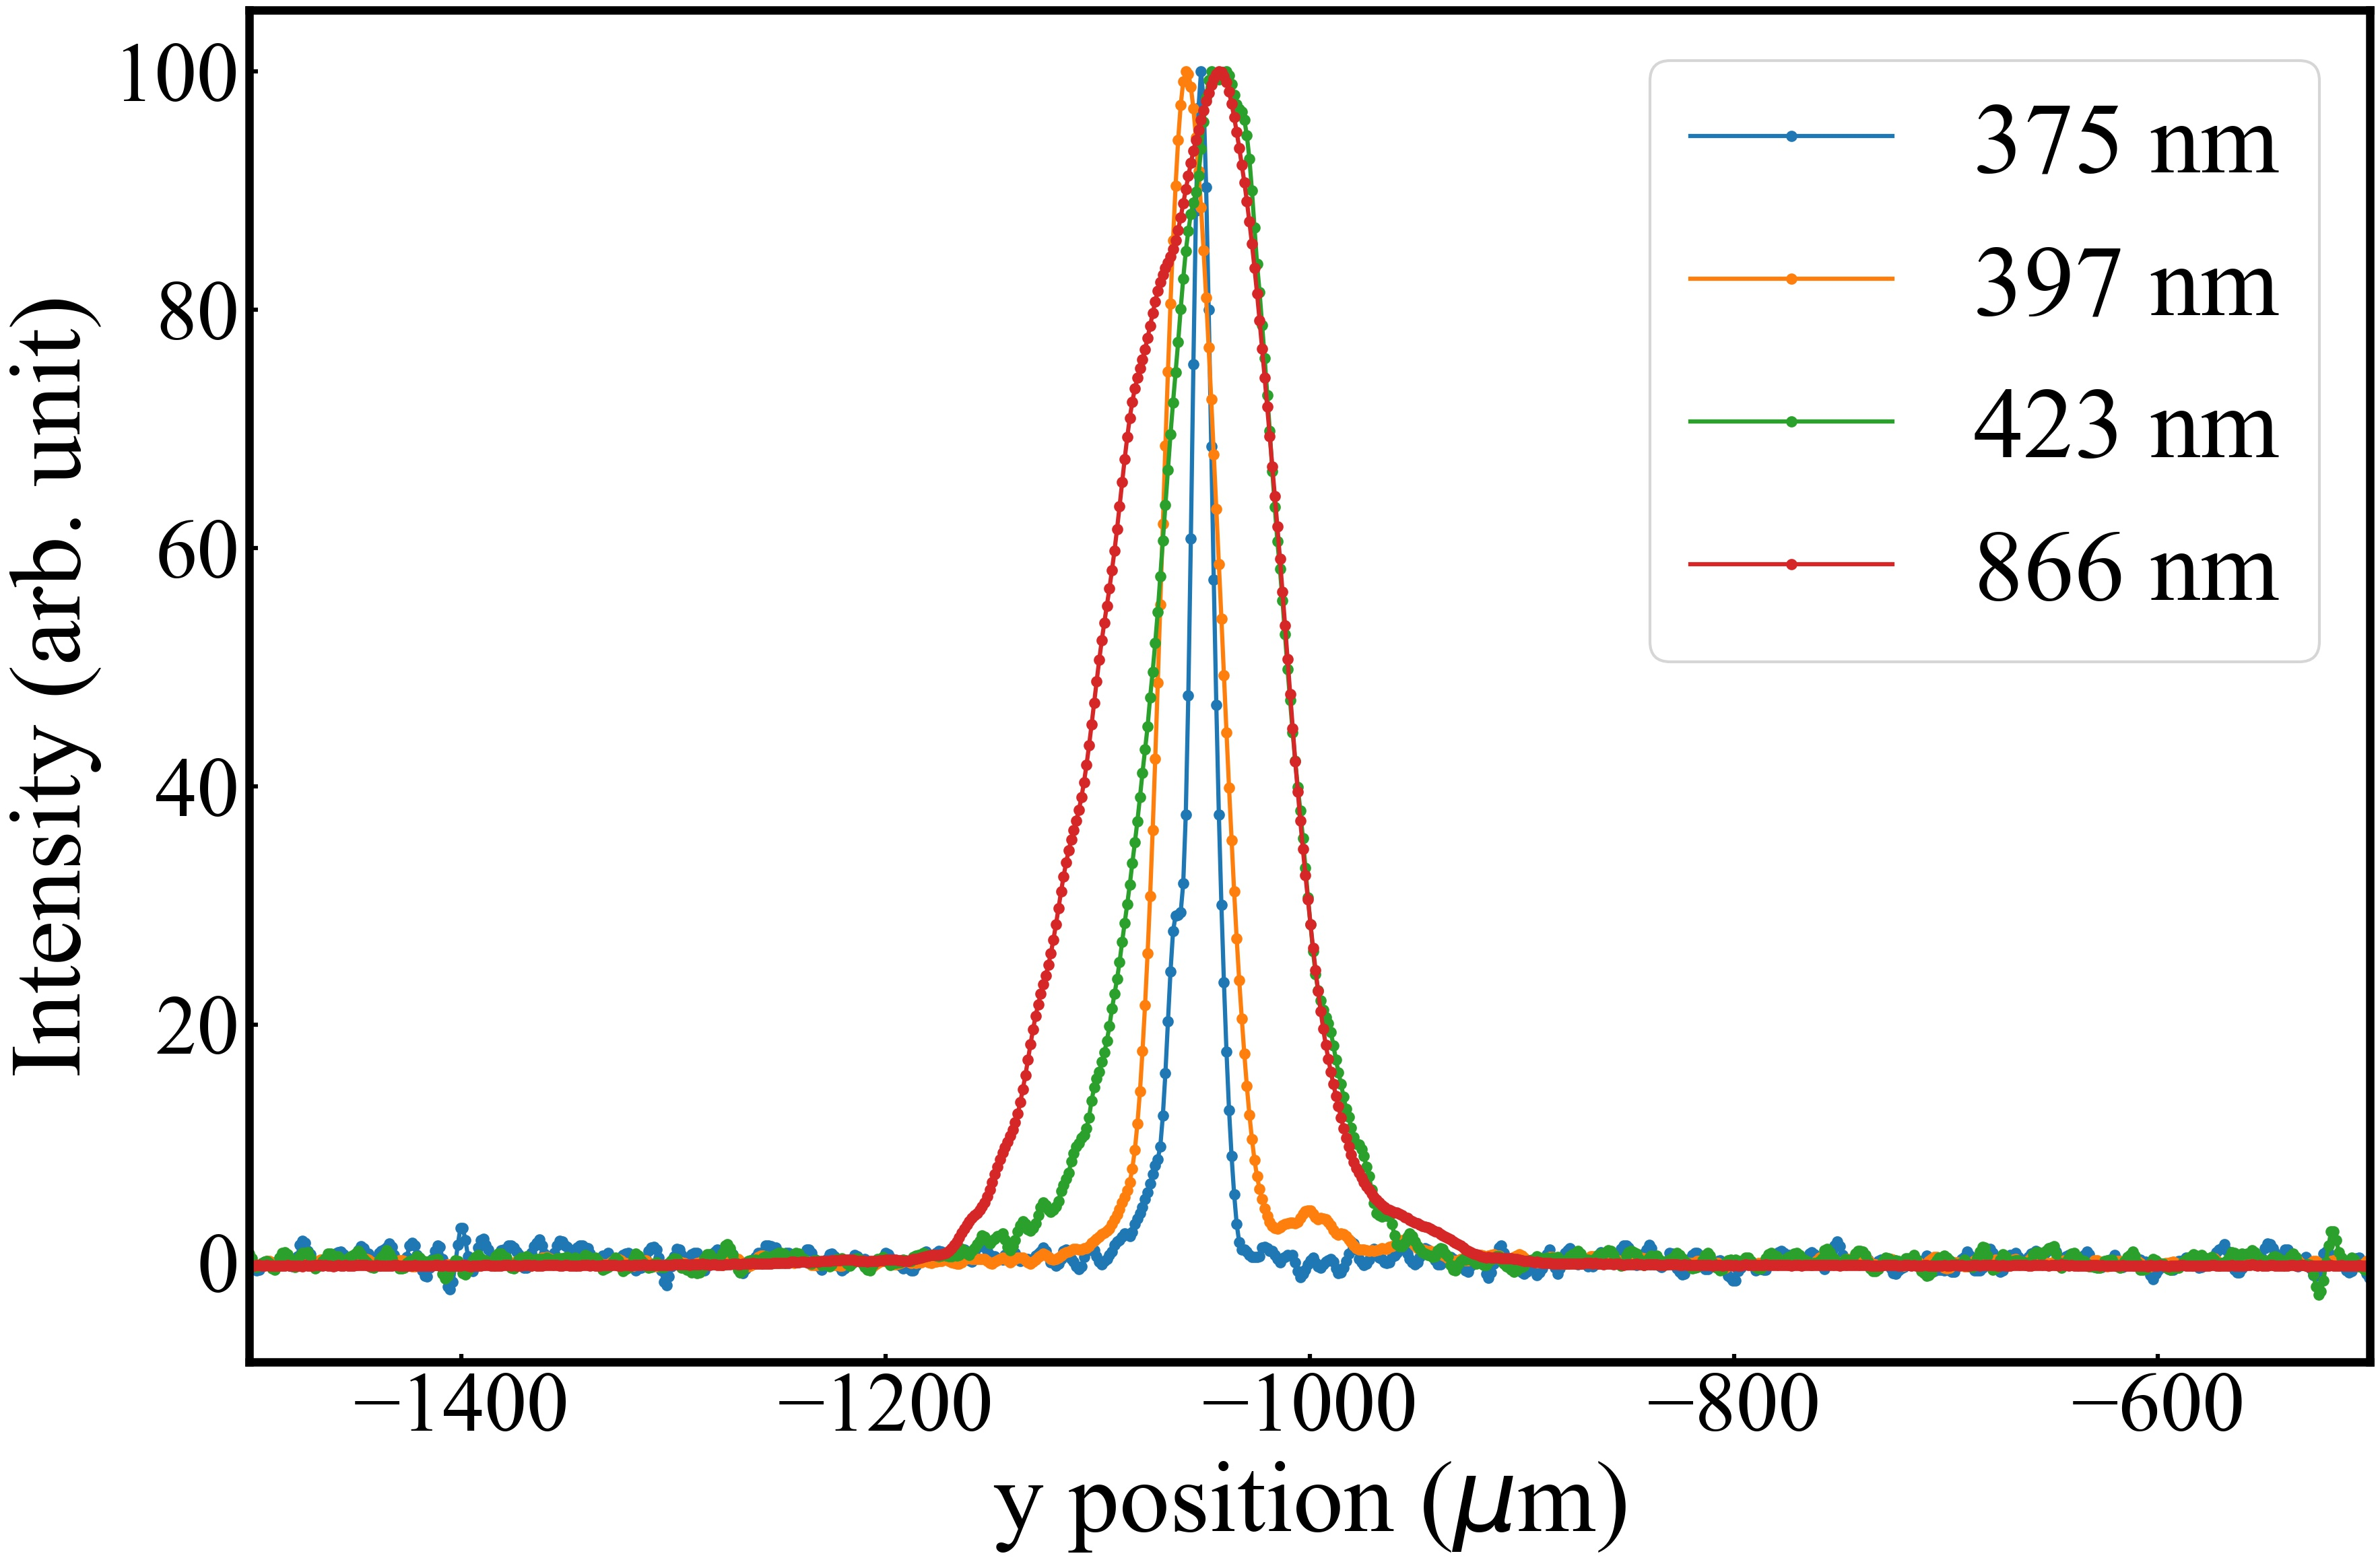
\includegraphics[width = 0.98\columnwidth]{./experimental_setup/figure/AllLaserYpos.jpg}
		\end{center}
	\end{minipage}
	\caption{4種類のレーザーのx,y方向についてのビームプロファイル結果}
	\label{fig:AllLaserBeamProfile}
	\end{center}
\end{figure}

そして,得られたビームプロファイルにガウシアンによるフィッティングを行った様子を\Fig{GaussianFitting}に示し,その結果を\Tb{GaussianFitting}にまとめている.\\

\begin{table}[h]
	\begin{center}
		\caption{ビームプロファイラで得られた各ビームのプロファイルにガウシアンフィッティングをかけて得られたパラメータ}
		\label{tab:GaussianFitting}
		\begin{tabular}{c|cc|cc} \hline \hline
			波長 (nm)&位置(x) ($\mu$m)&ビーム径(x) ($\mu$m) &位置(y) ($\mu$m)& ビーム径(y) ($\mu$m)\\ \hline
			375&-2600.82$\pm$0.035&6.96$\pm$0.049&-1051.14$\pm$0.028&9.37$\pm$0.04 \\
			397&-2606.08$\pm$0.026&24.21$\pm$0.037&-1056.17$\pm$0.016&18.45$\pm$0.023 \\
			423&-2611.55$\pm$0.05&30.20$\pm$0.072&1042.25$\pm$0.03&39.85$\pm$0.054 \\
			866&-2606.08$\pm$0.138&77.20$\pm$0.196&-1054.24$\pm$0.06&54.72$\pm$0.085 \\\hline
		\end{tabular}
	\end{center}
\end{table}

\clearpage

\begin{figure}[h]
	\begin{center}
	%%%12
	\begin{minipage}{0.48\linewidth}
	\begin{center}
			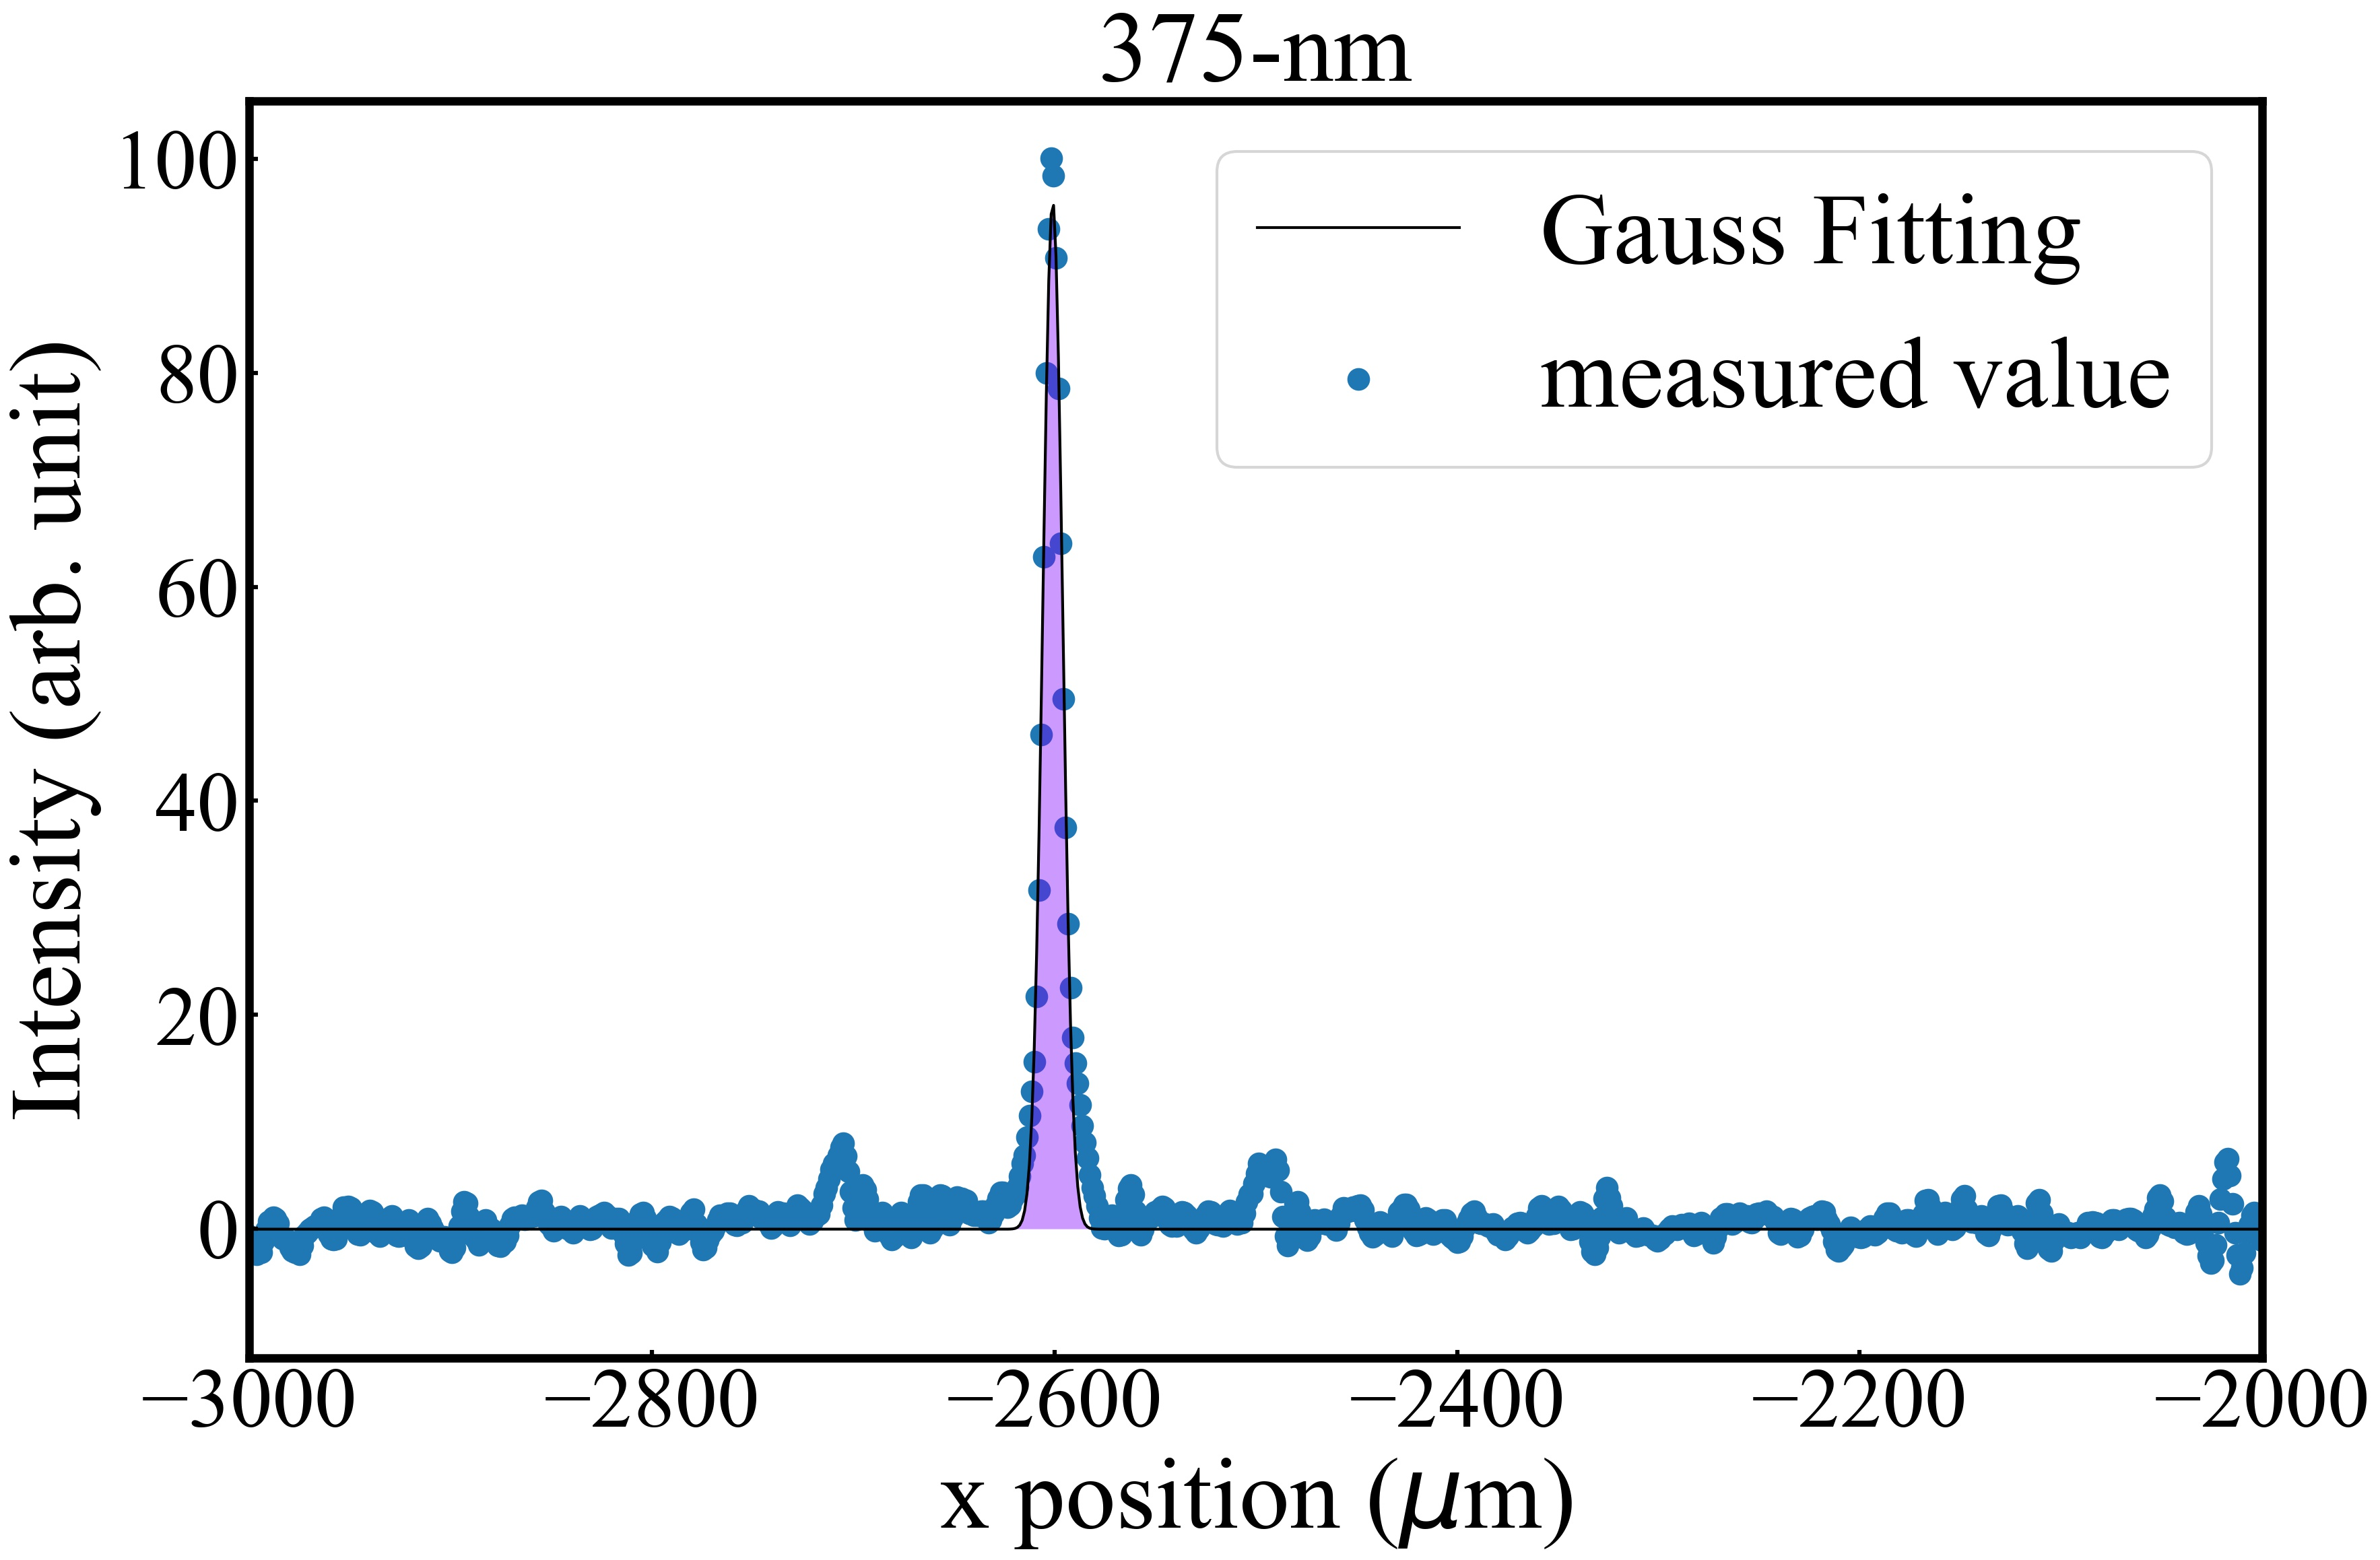
\includegraphics[width = 0.98\columnwidth]{./experimental_setup/figure/375GaussianFittingXpos.jpg}
	\end{center}
	\end{minipage}
	\begin{minipage}{0.48\linewidth}
	\begin{center}
			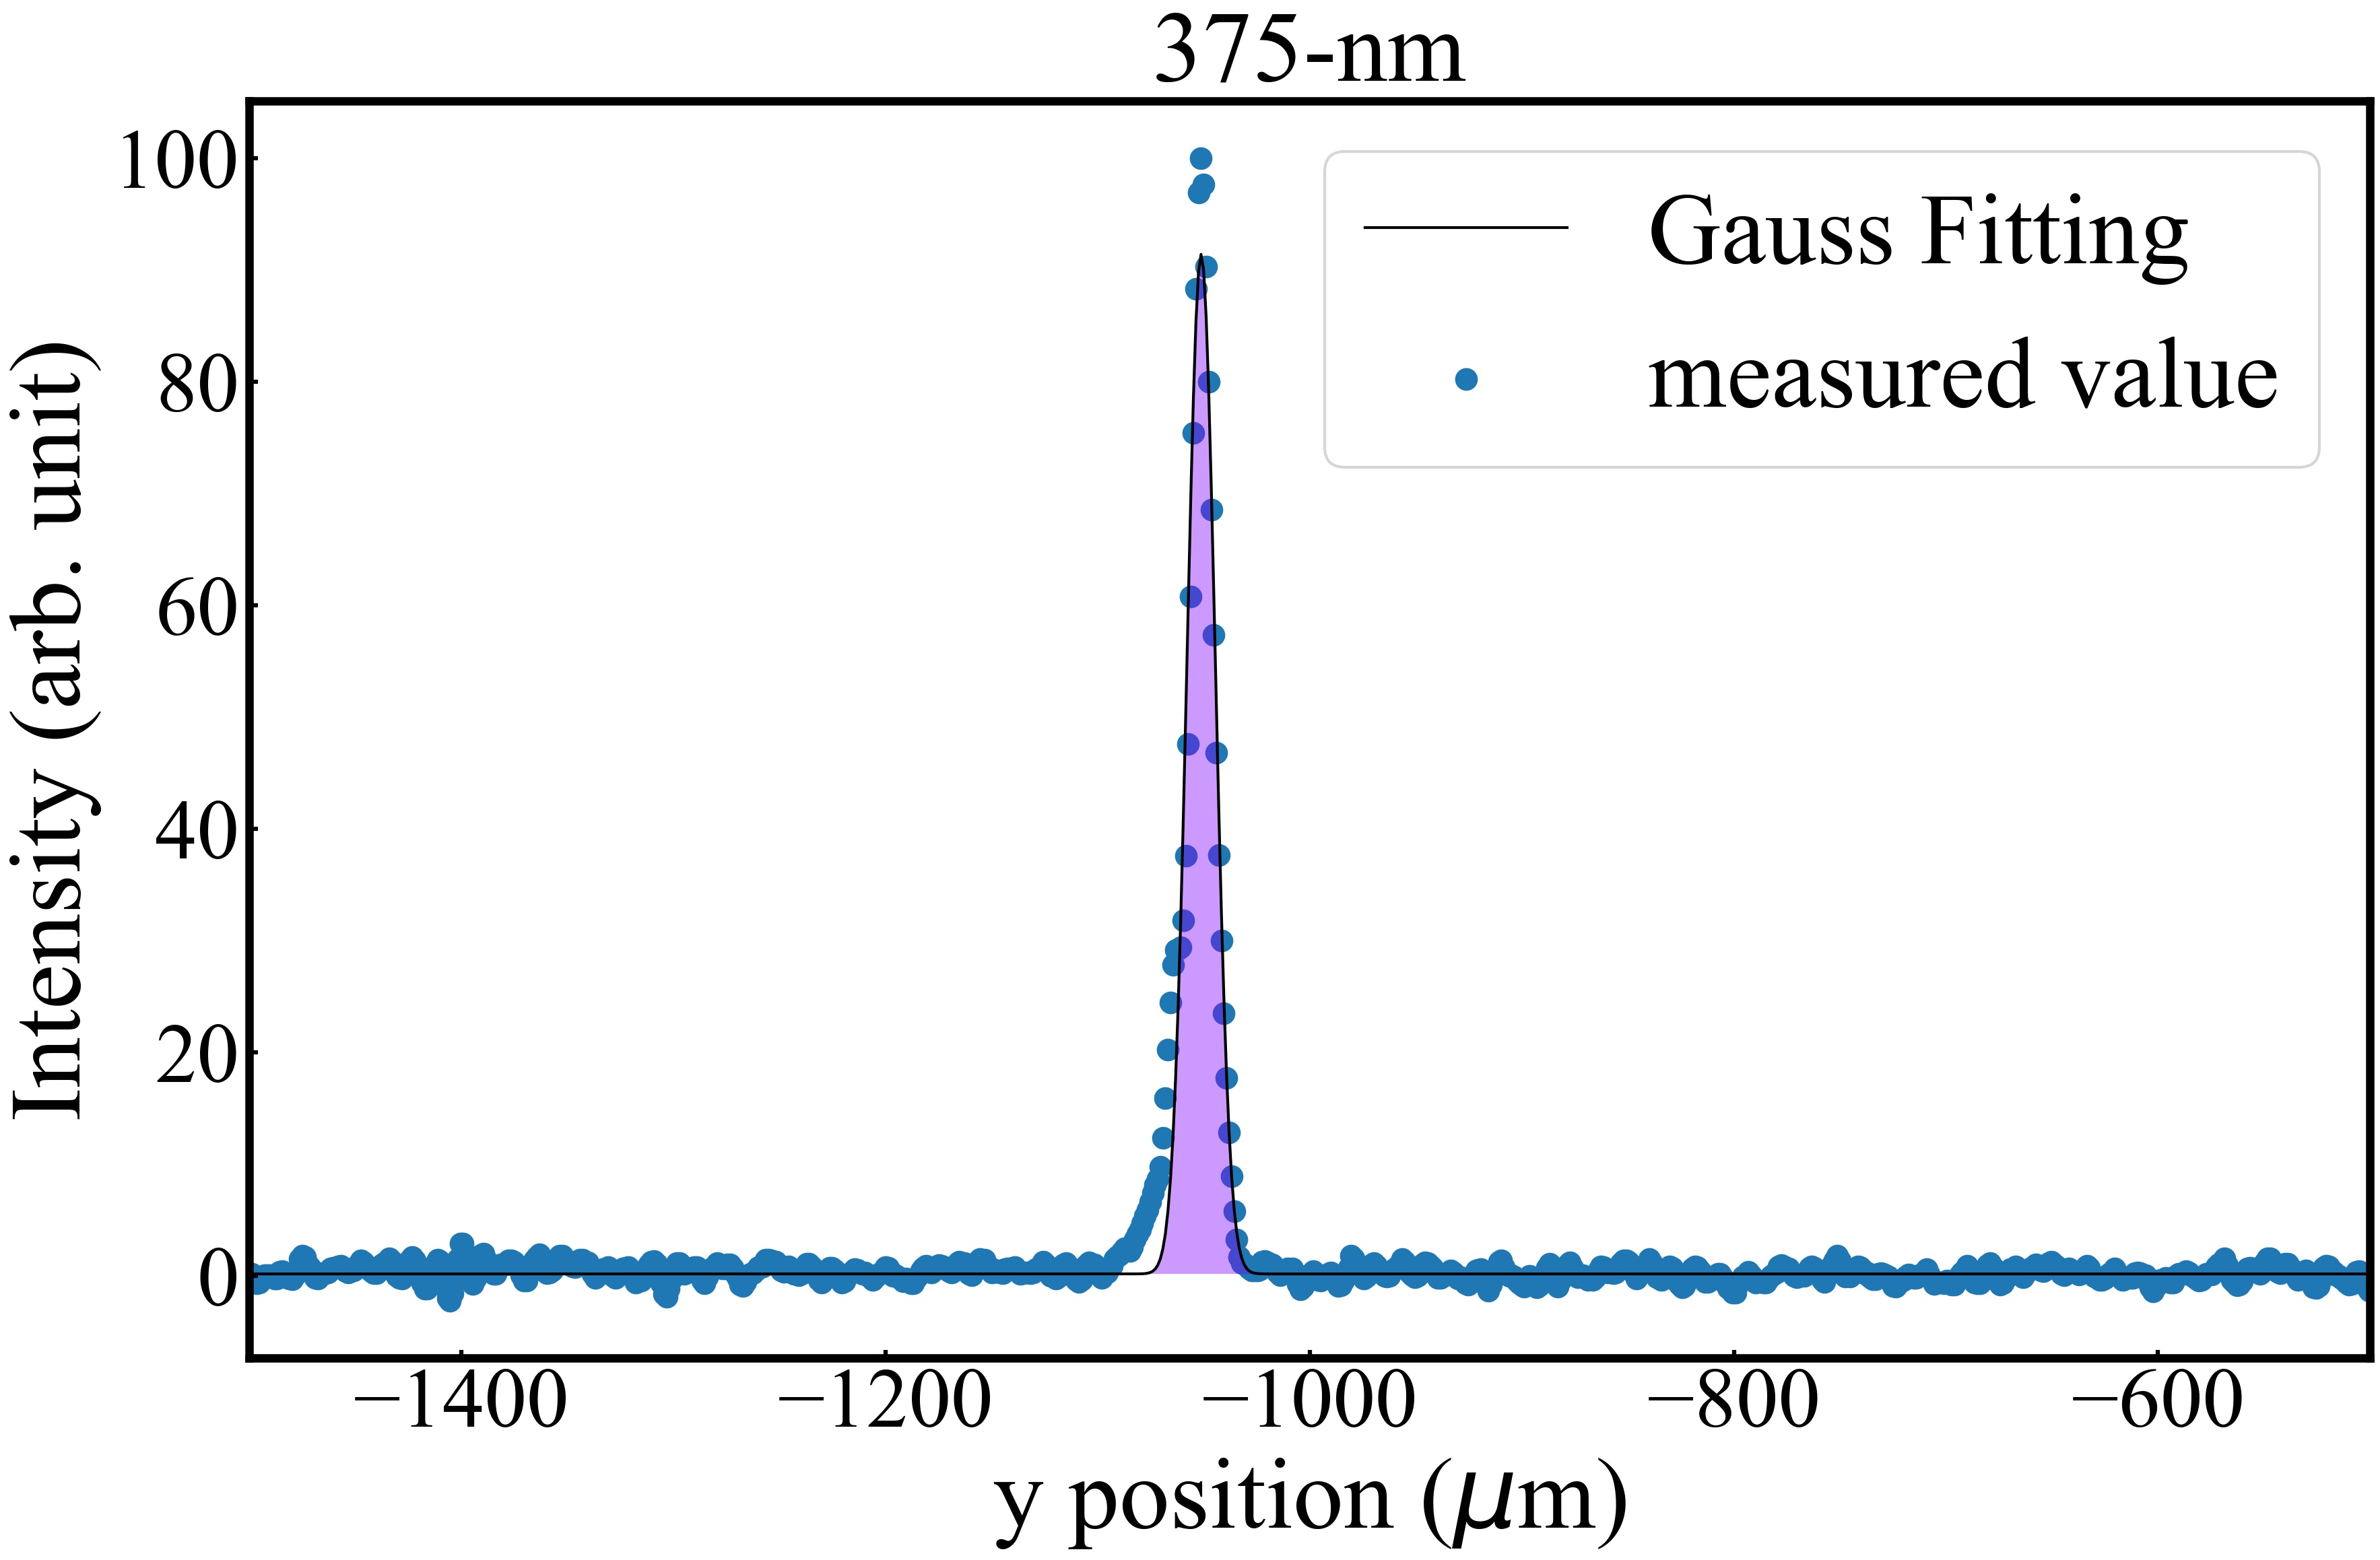
\includegraphics[width=0.98\columnwidth]{./experimental_setup/figure/375GaussianFittingYpos.jpg}
	\end{center}
	\end{minipage}
	%%%34
	\begin{minipage}{0.48\linewidth}
	\begin{center}
		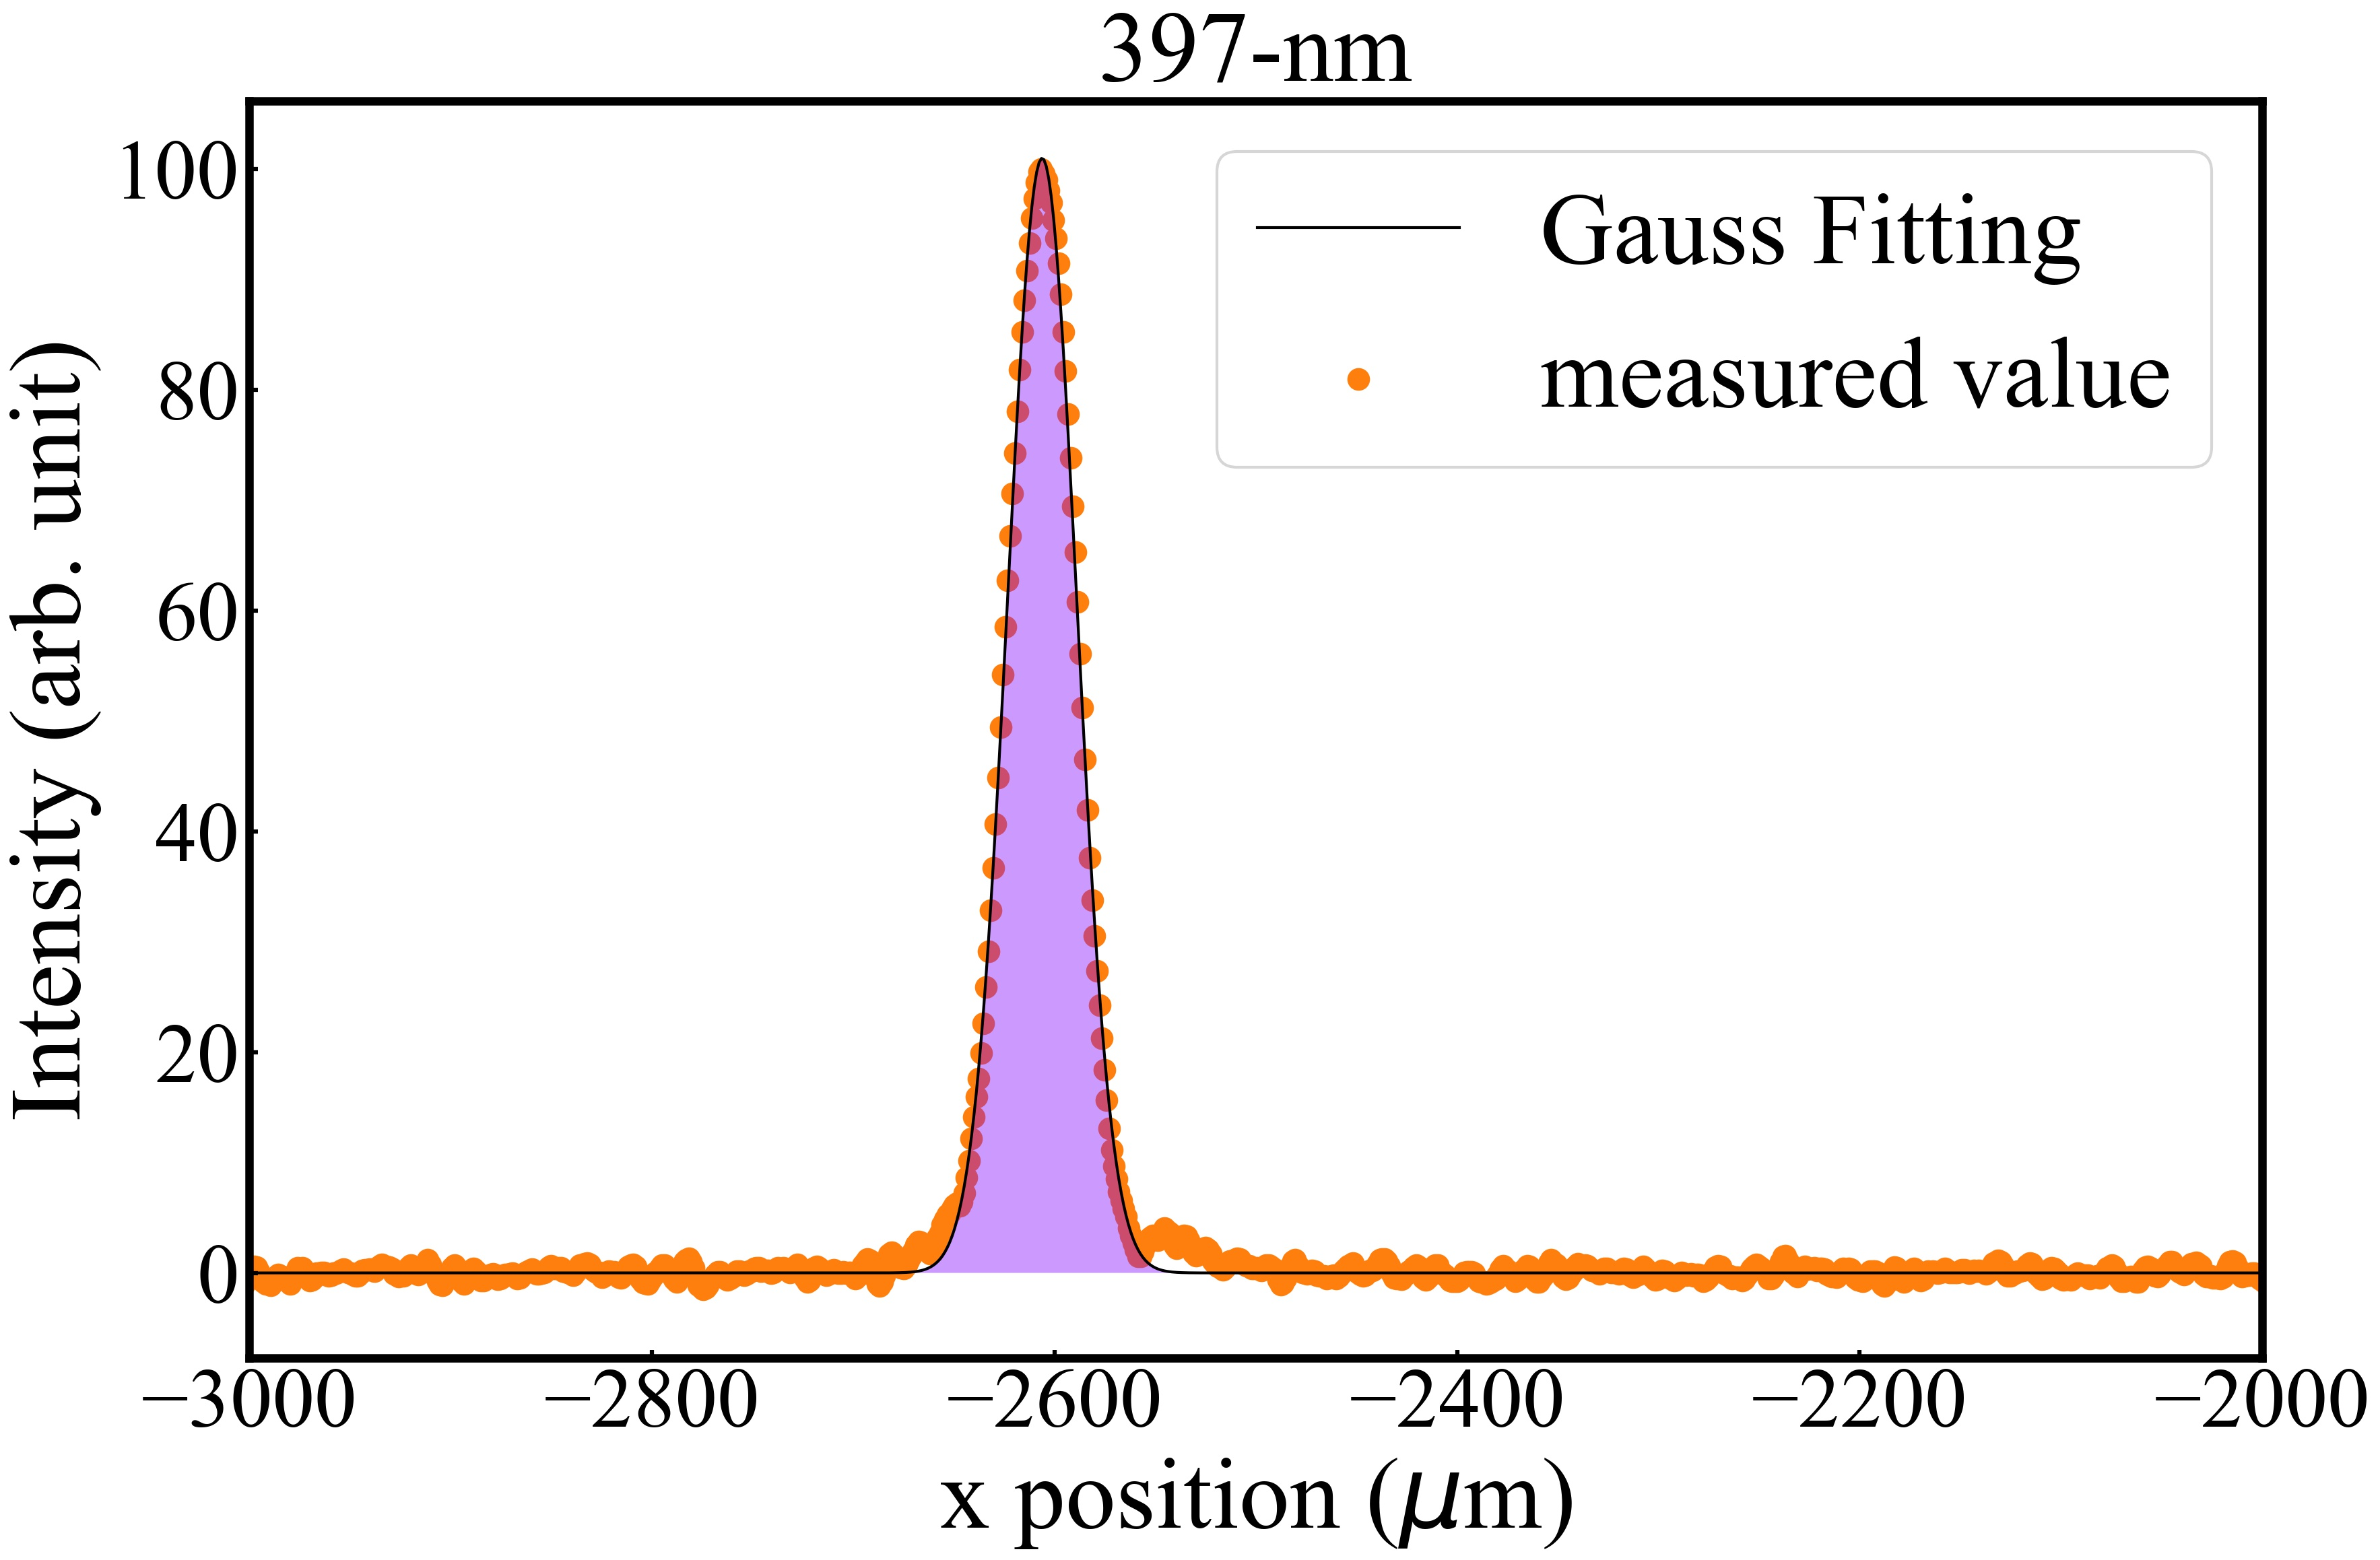
\includegraphics[width = 0.98\columnwidth]{./experimental_setup/figure/397GaussianFittingXpos.jpg}
	\end{center}
	\end{minipage}
	\begin{minipage}{0.48\linewidth}
	\begin{center}
		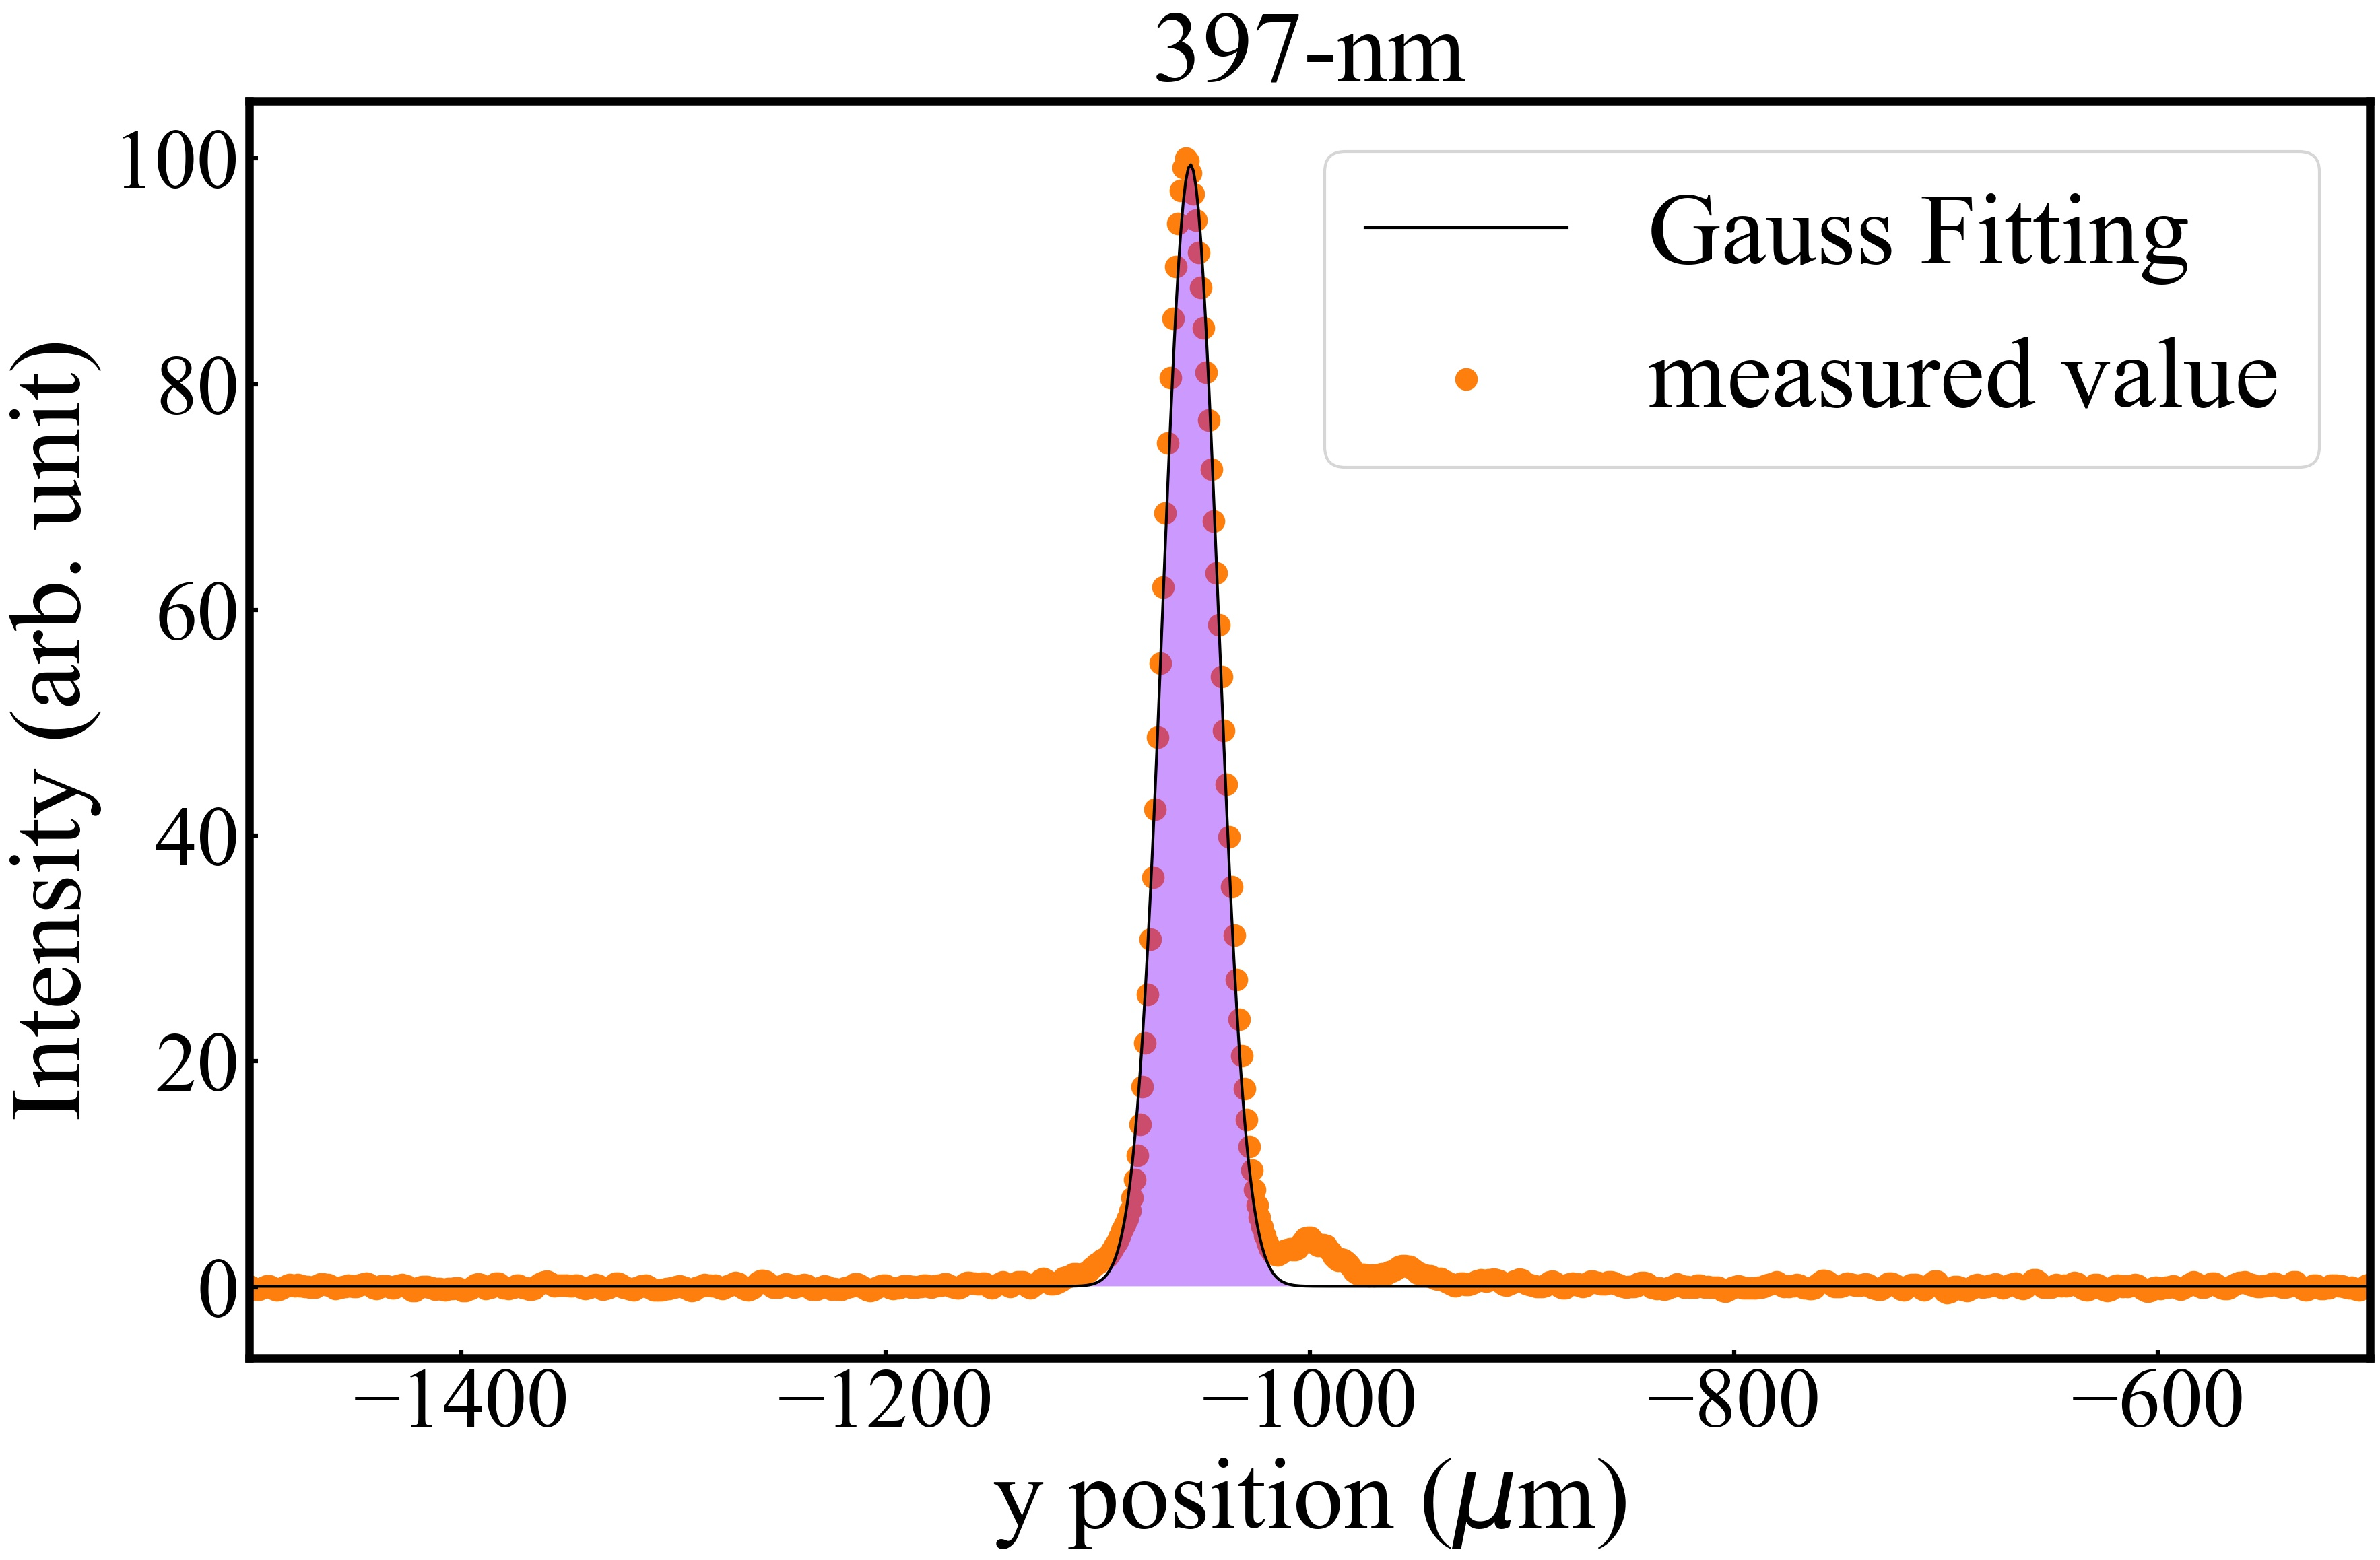
\includegraphics[width=0.98\columnwidth]{./experimental_setup/figure/397GaussianFittingYpos.jpg}
	\end{center}
	\end{minipage}
	%%%56
	\begin{minipage}{0.48\linewidth}
	\begin{center}
		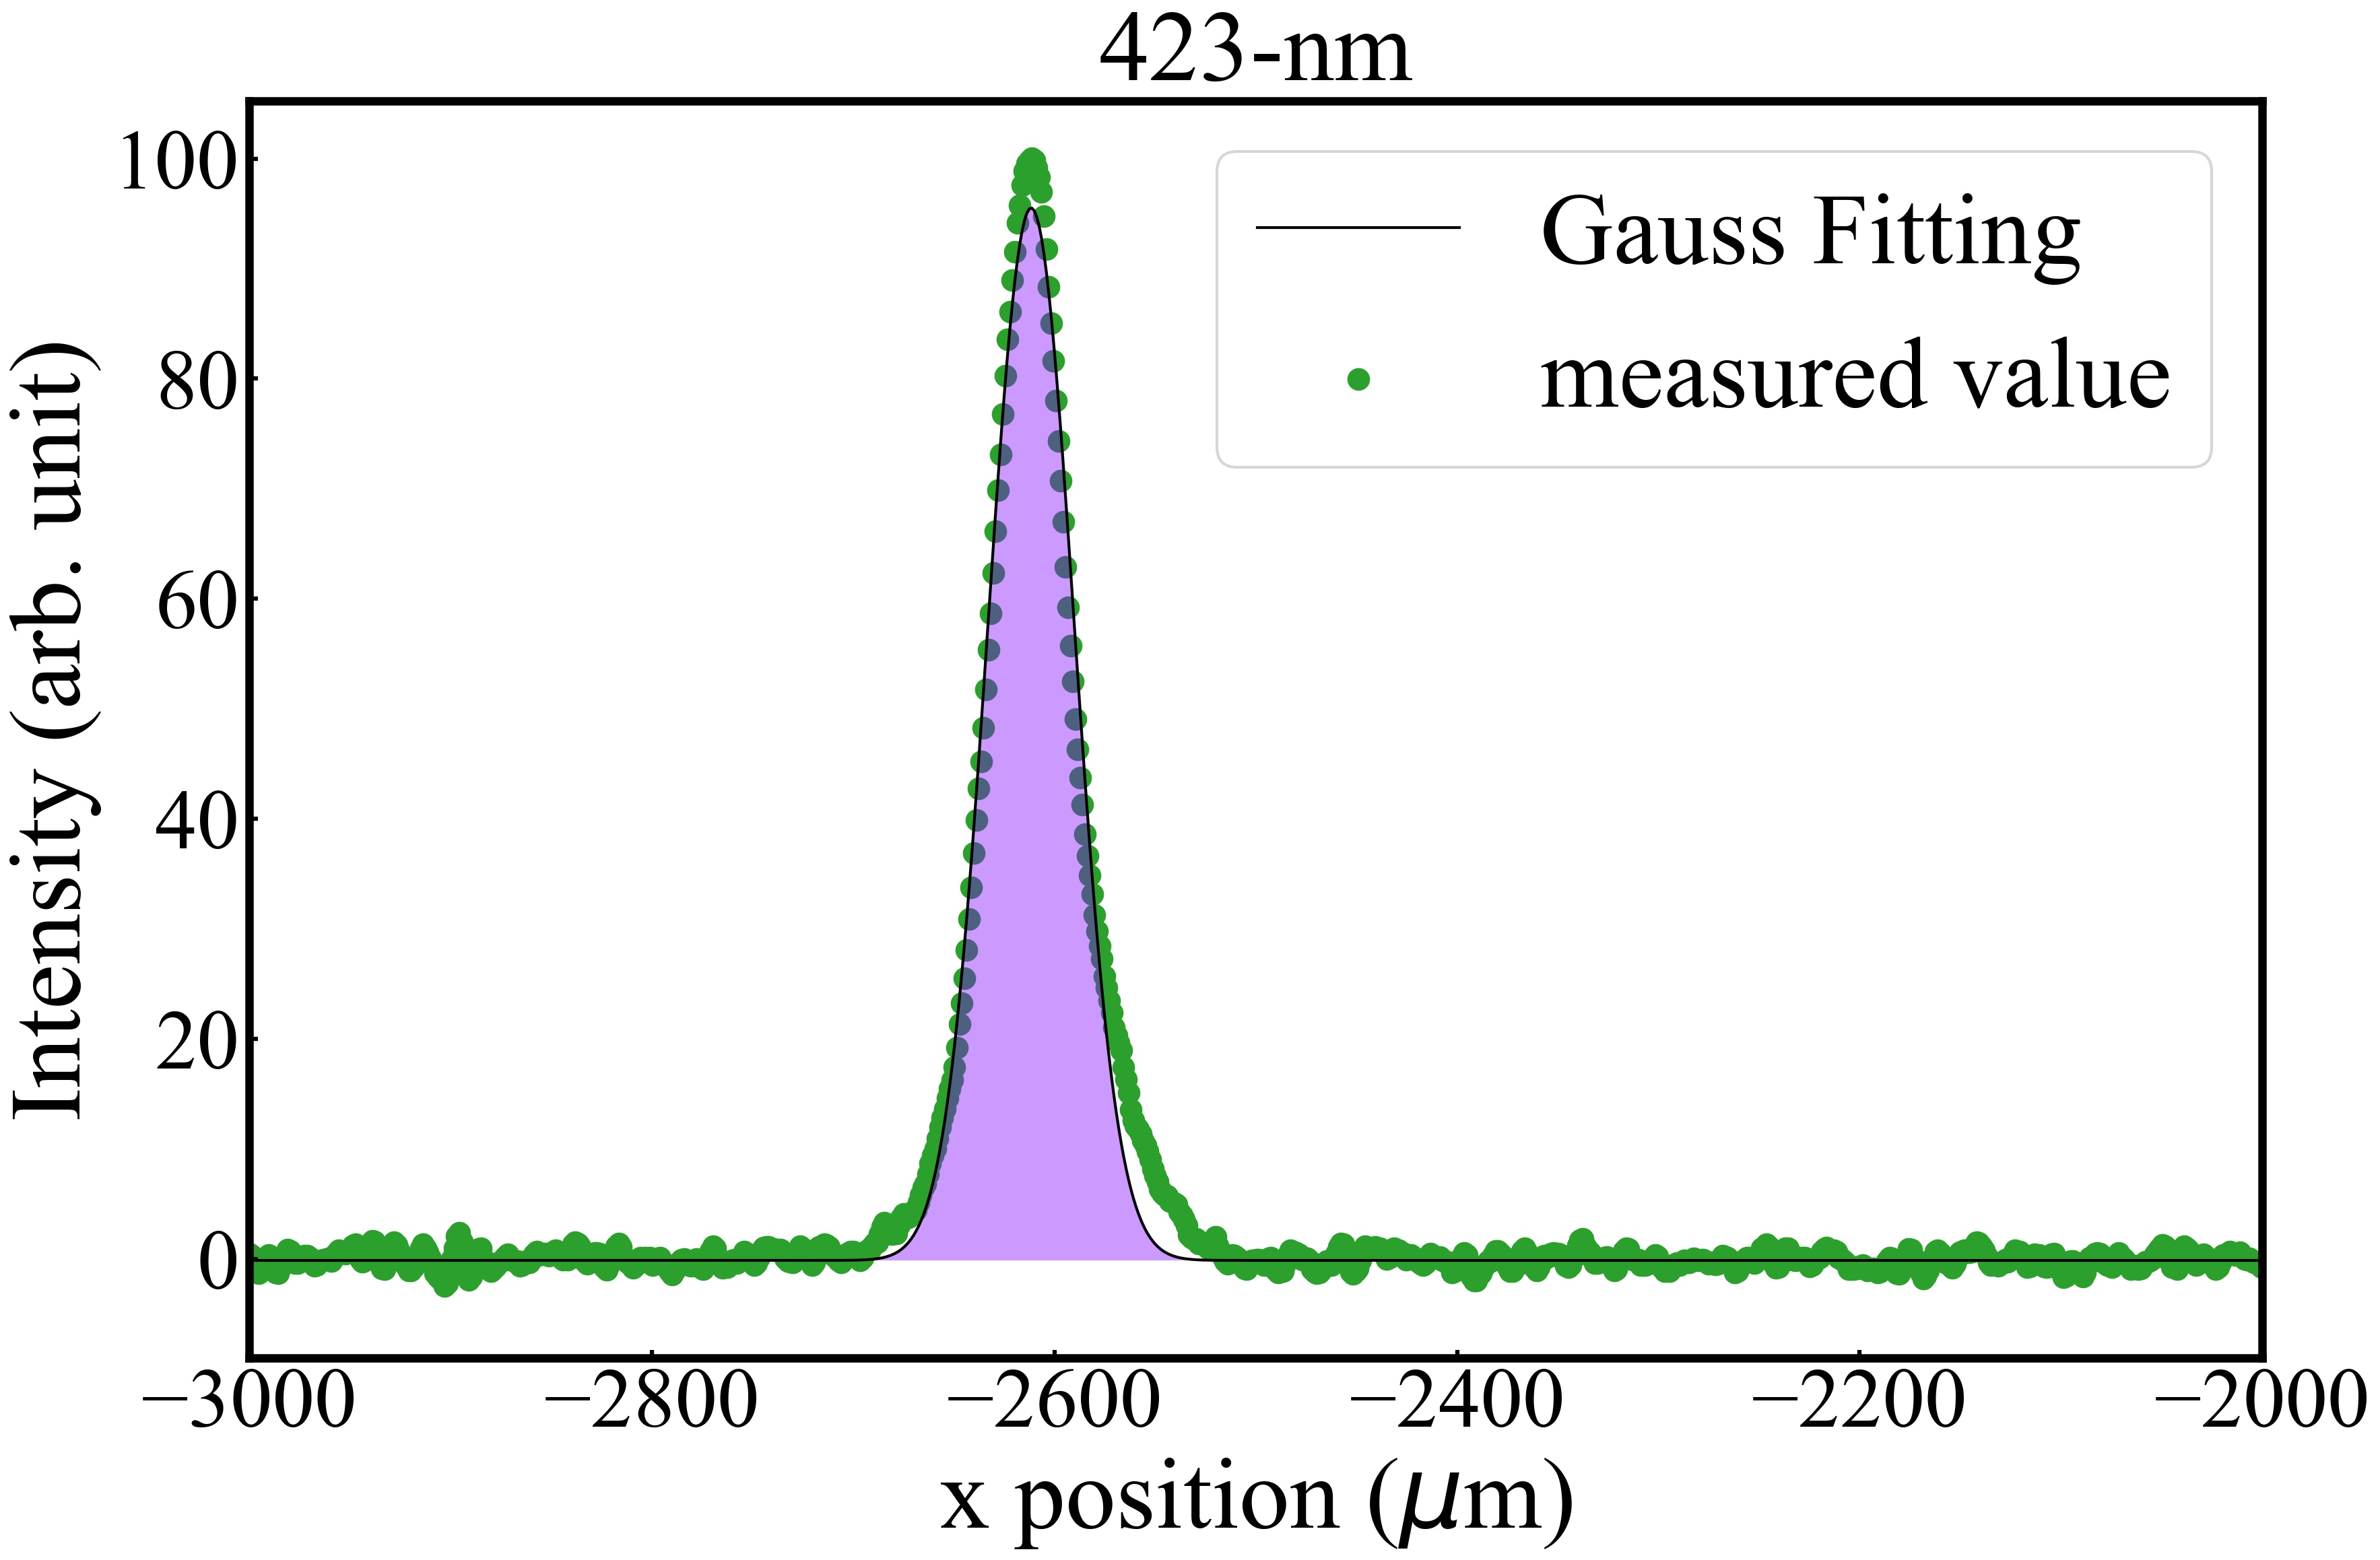
\includegraphics[width = 0.98\columnwidth]{./experimental_setup/figure/423GaussianFittingXpos.jpg}
	\end{center}
	\end{minipage}
	\begin{minipage}{0.48\linewidth}
	\begin{center}
		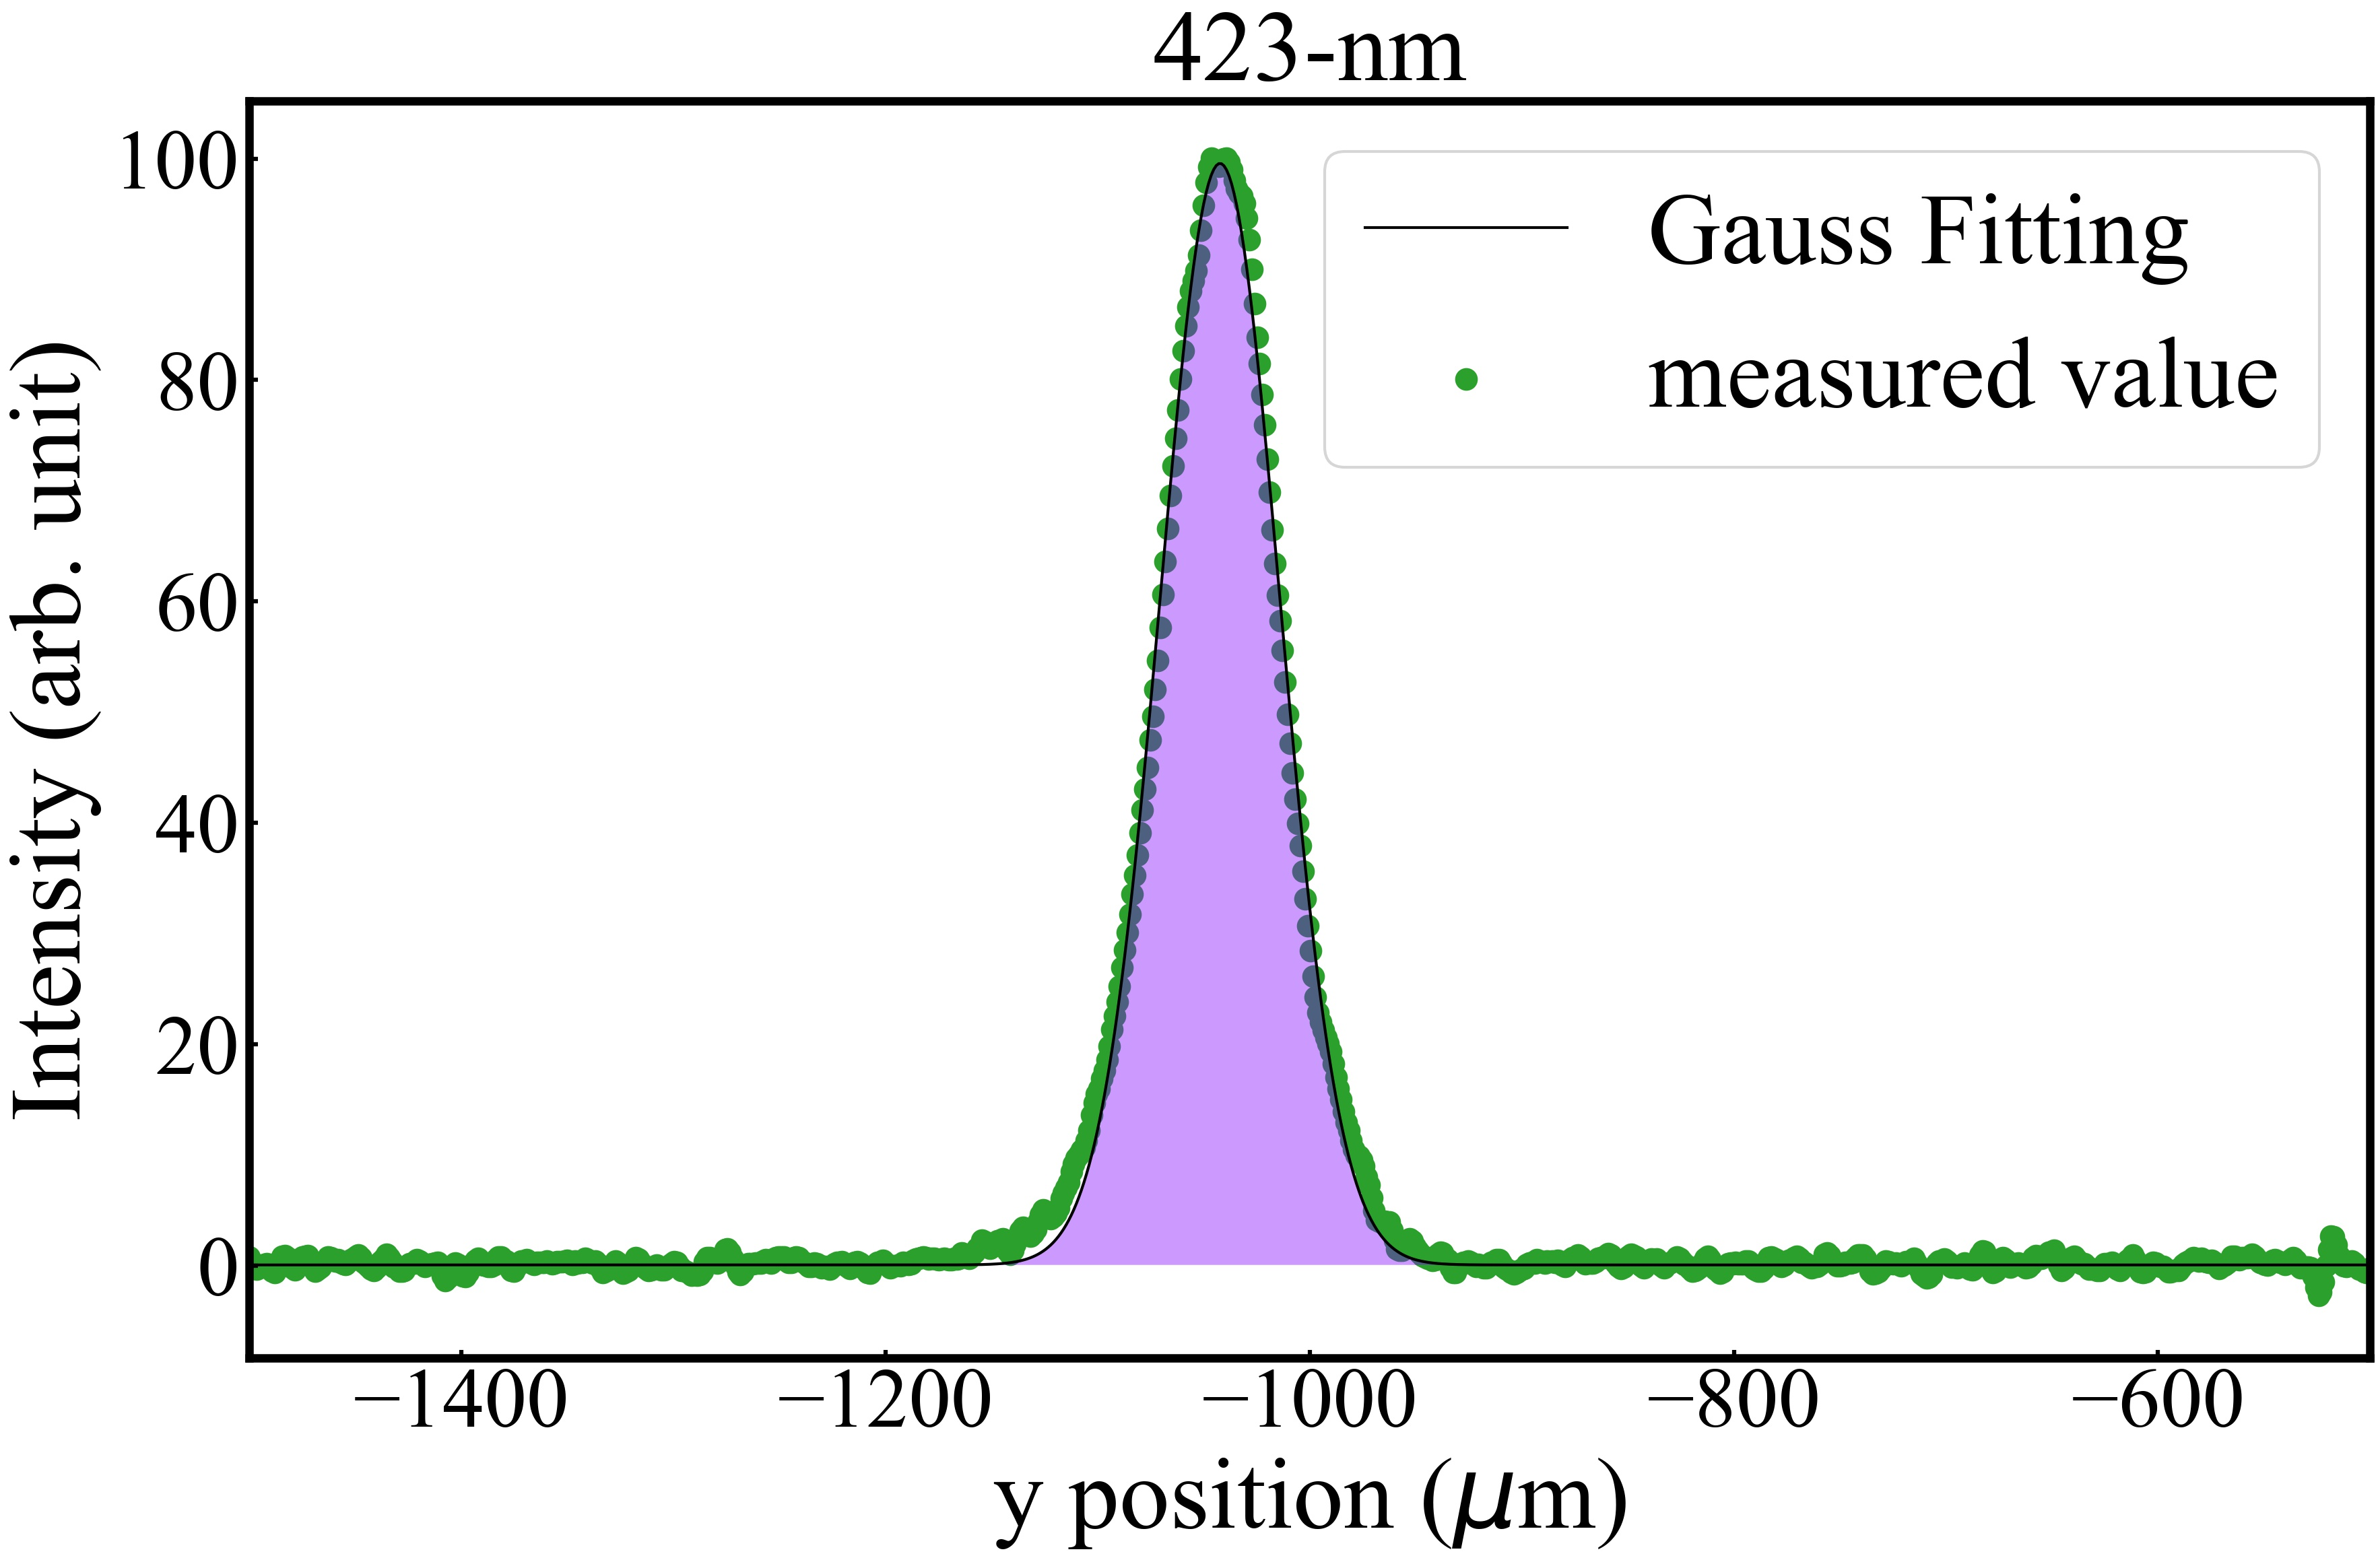
\includegraphics[width=0.98\columnwidth]{./experimental_setup/figure/423GaussianFittingYpos.jpg}
	\end{center}
	\end{minipage}
	%%%78
	\begin{minipage}{0.48\linewidth}
	\begin{center}
		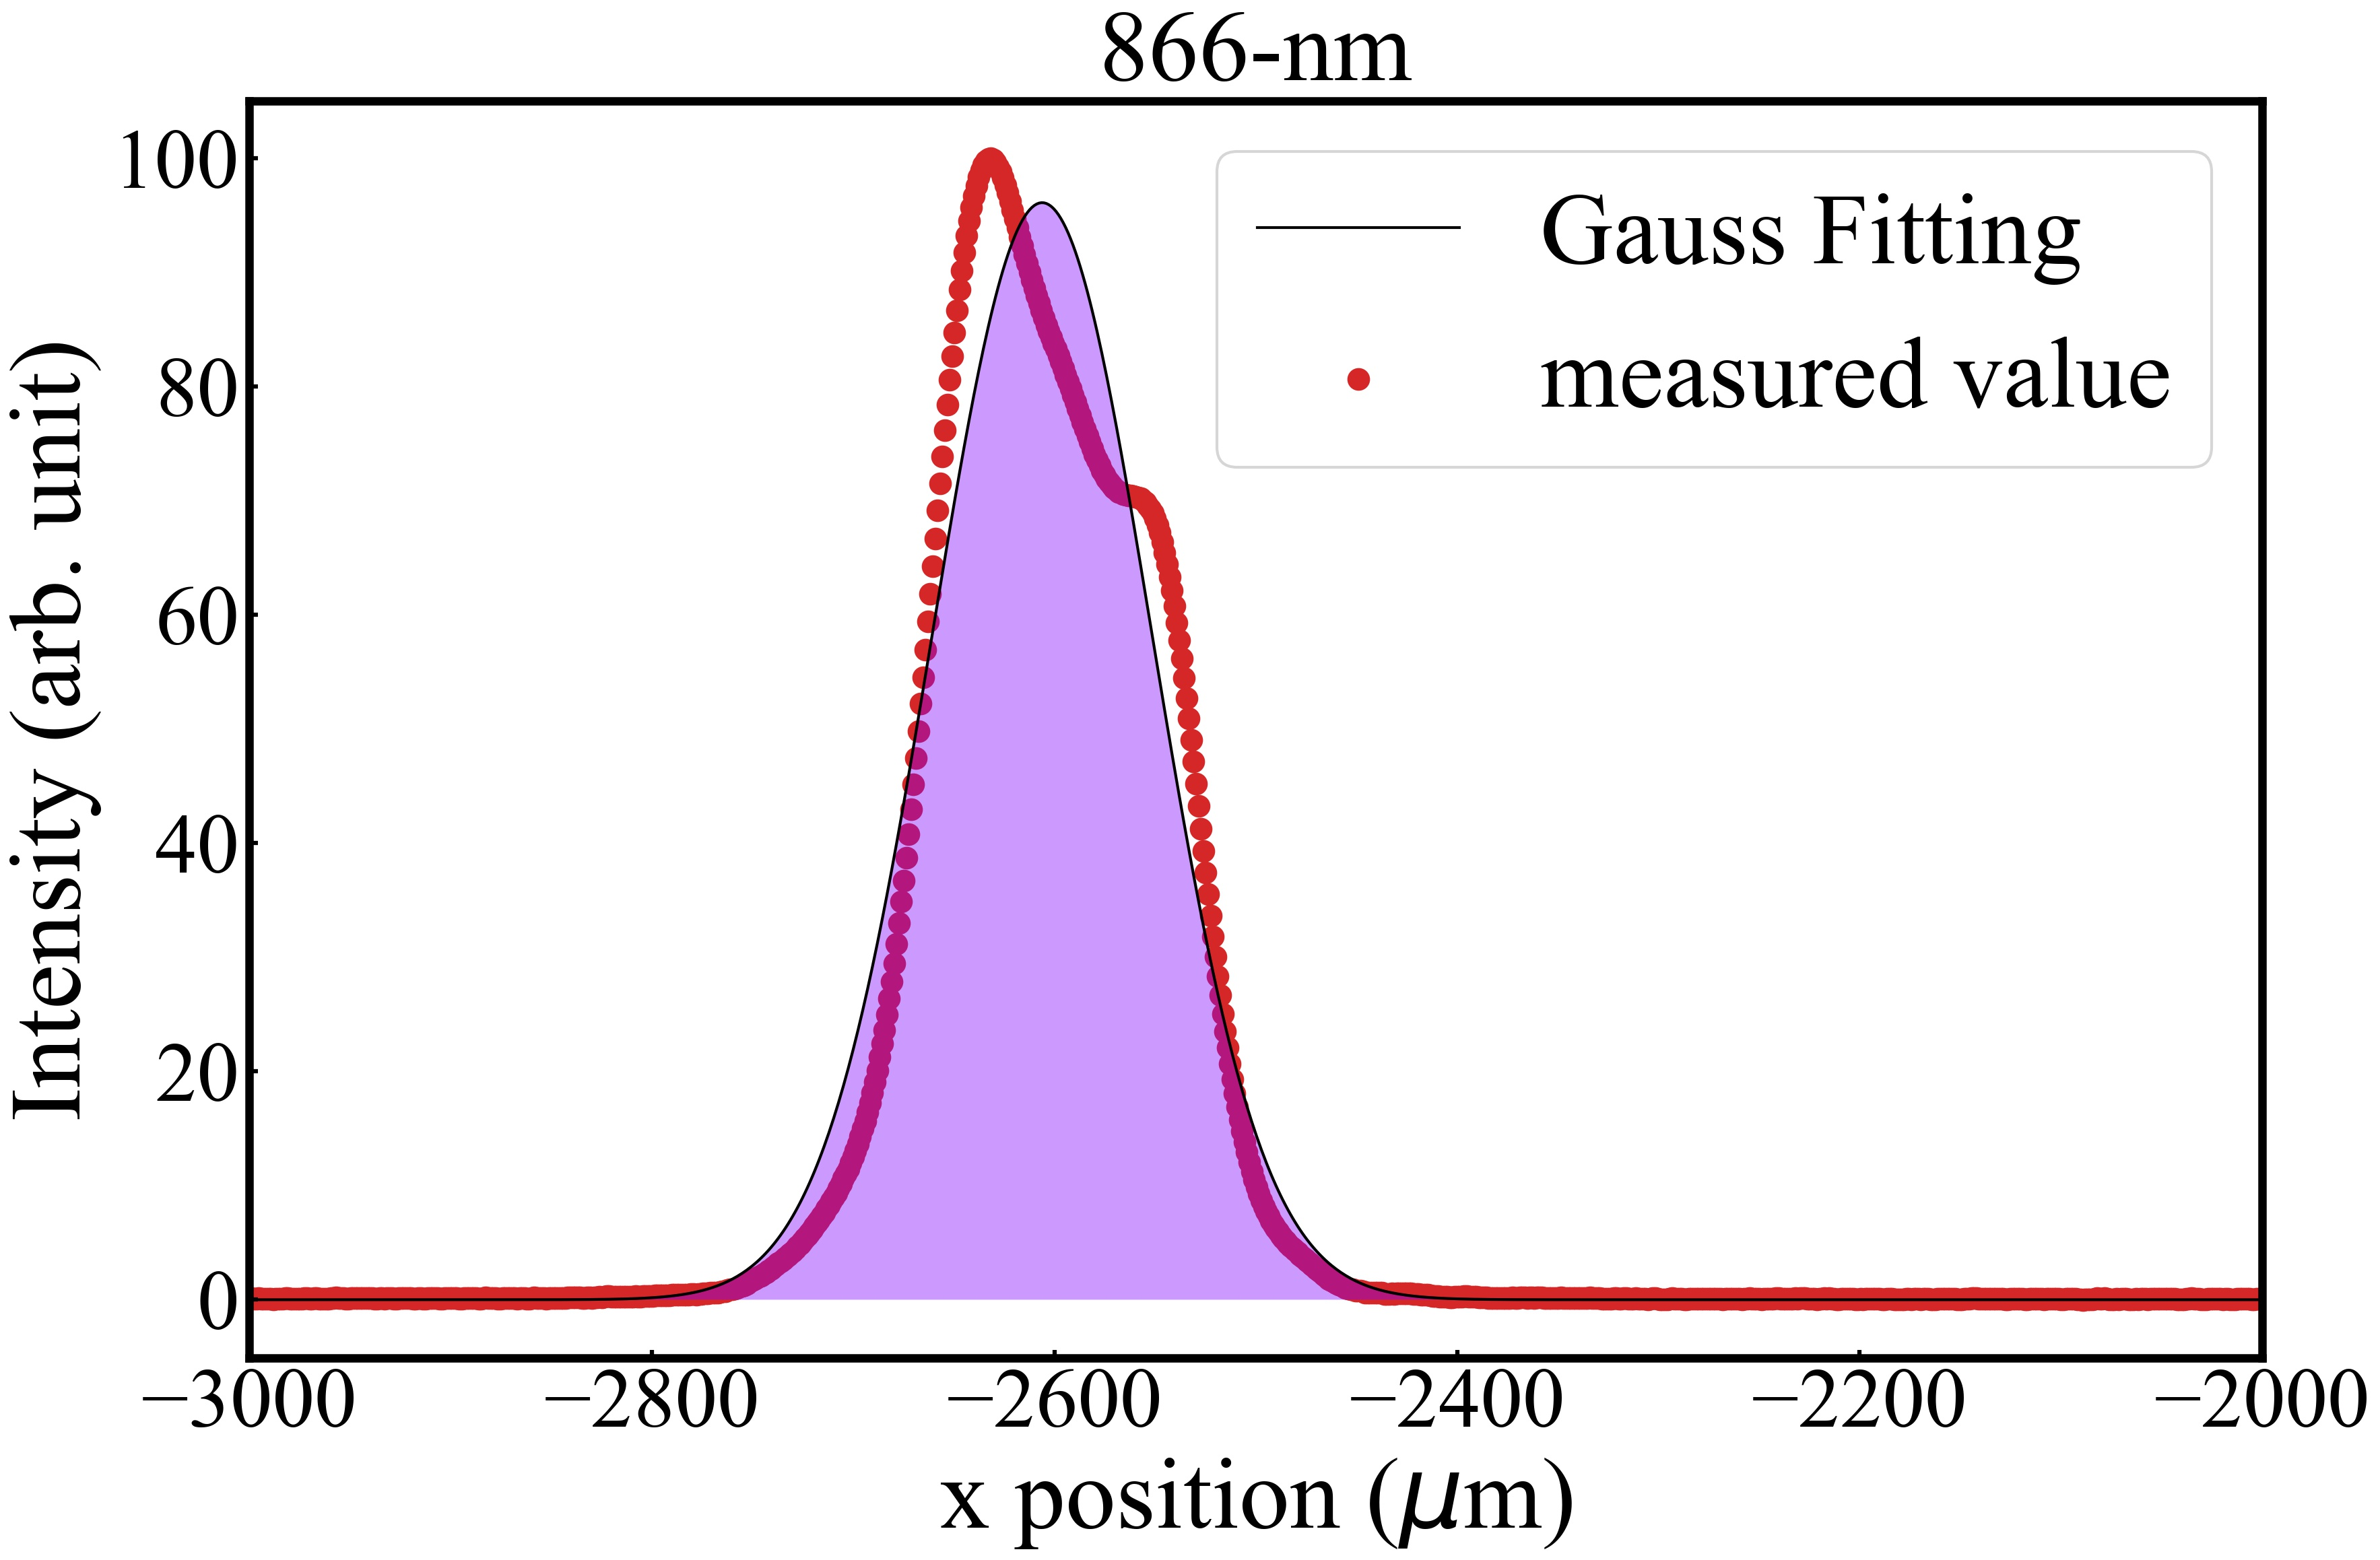
\includegraphics[width = 0.98\columnwidth]{./experimental_setup/figure/866GaussianFittingXpos.jpg}
	\end{center}
	\end{minipage}
	\begin{minipage}{0.48\linewidth}
	\begin{center}
		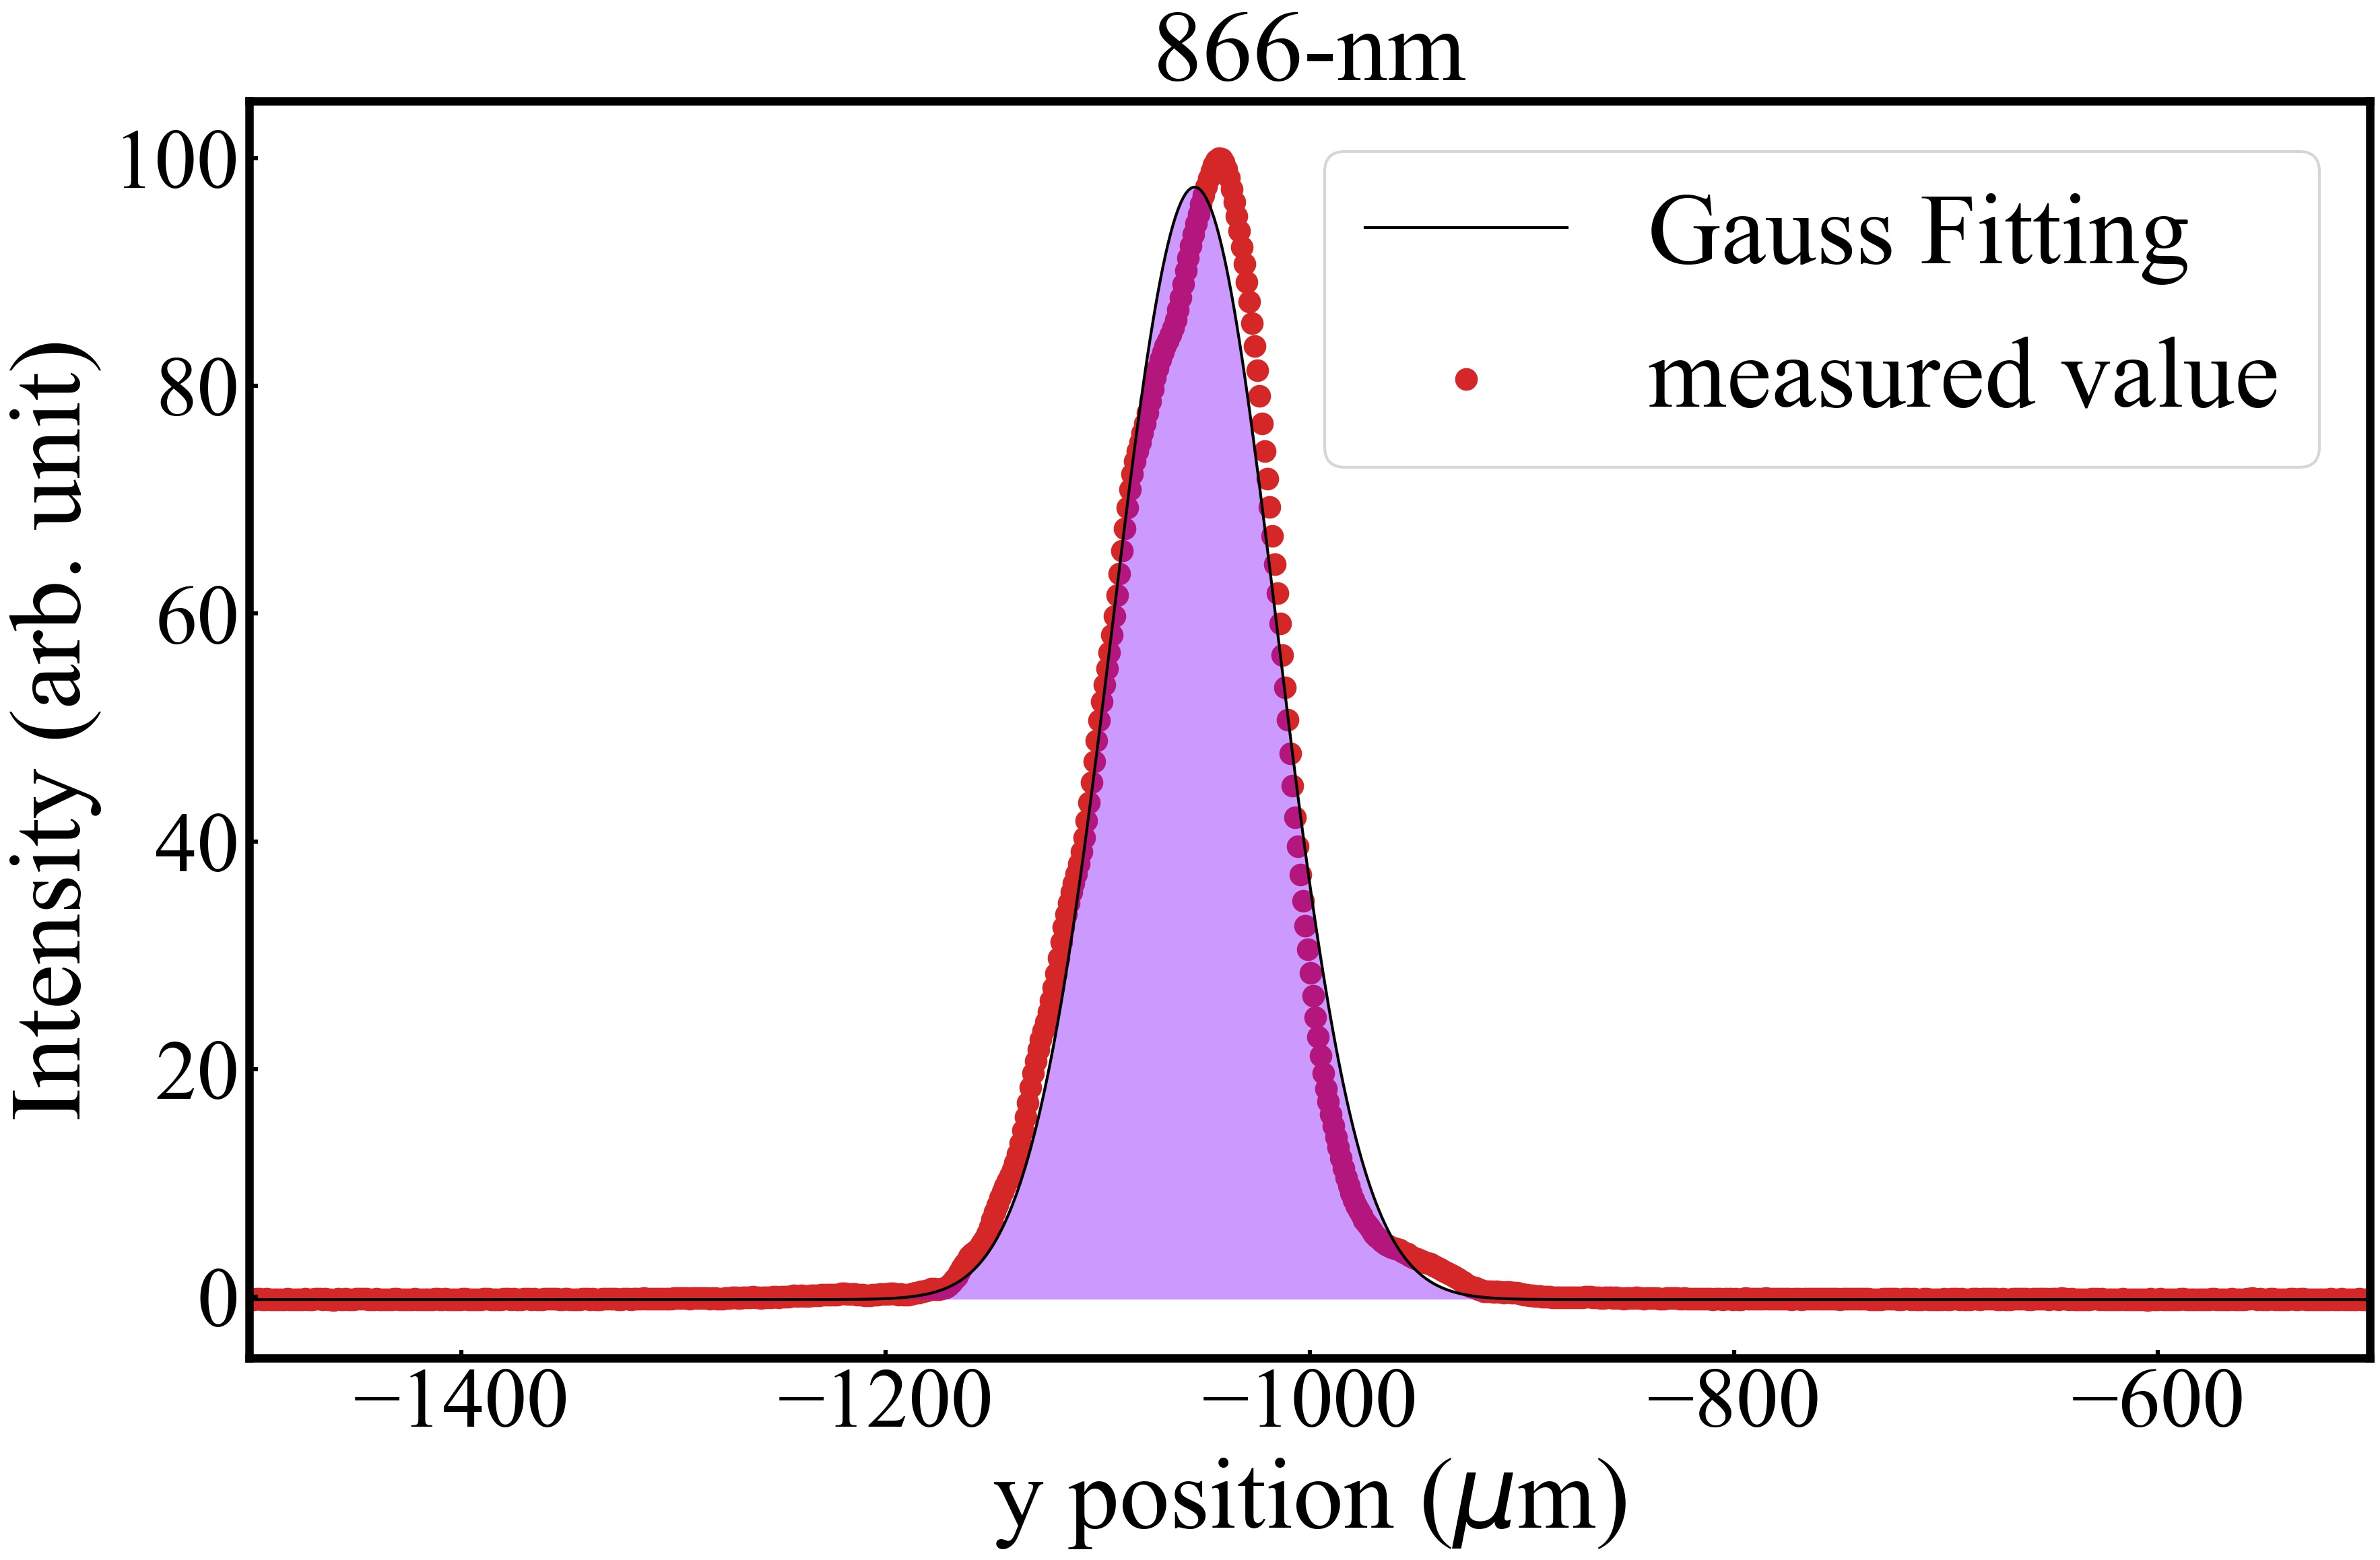
\includegraphics[width = 0.98\columnwidth]{./experimental_setup/figure/866GaussianFittingYpos.jpg}
	\end{center}
	\end{minipage}
	\caption{各波長に対してx,y方向それぞれのビームプロファイルにガウシアンフィッティングをかけた結果}
	\label{fig:GaussianFitting}
	\end{center}
\end{figure}
	% -- シミュレーション結果 -- %
	\chapter{シミュレーション結果}
\section{DCポテンシャル}
\Eq{rectangle_electrode}より,dc電圧を計算するためには電極モデルを矩形の形に分割する必要がある.Mathematica上における電極の分割の様子を\Fig{rect_electrode}に示す.
\begin{figure}[h]
	\begin{center}
		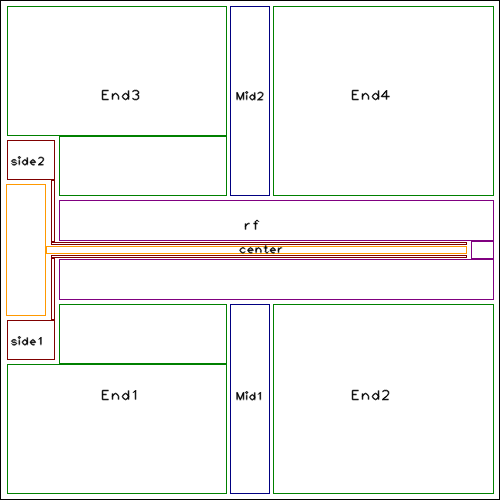
\includegraphics[width = 0.4\linewidth]{./simulation/figure/named_rect_electrode.png}
	\end{center}
	\caption{a}
	\label{fig:rect_electrode}
\end{figure}
各dc電極によってプレーナートラップ上の点$(x,y,z)$に形成される静電ポテンシャル$\Phi_{\rm DC}(x,y,z)$は,分割した各矩形が$(x,y,z)$に形成する静電ポテンシャルの重ね合わせで
\large
\begin{align}
	\Phi_{\rm DC}(x,y,z) = \phi_{\rm End1} + \phi_{\rm End2} + \phi_{\rm End3} &+ \phi_{\rm End4} + \phi_{\rm Mid1} + \phi_{\rm Mid2} \notag \\
	&+ \phi_{\rm Side1} + \phi_{\rm Side2} + \phi_{\rm center},
\end{align}
\normalsize
と表すことができる.
\begin{figure}[h]
	\begin{center}
		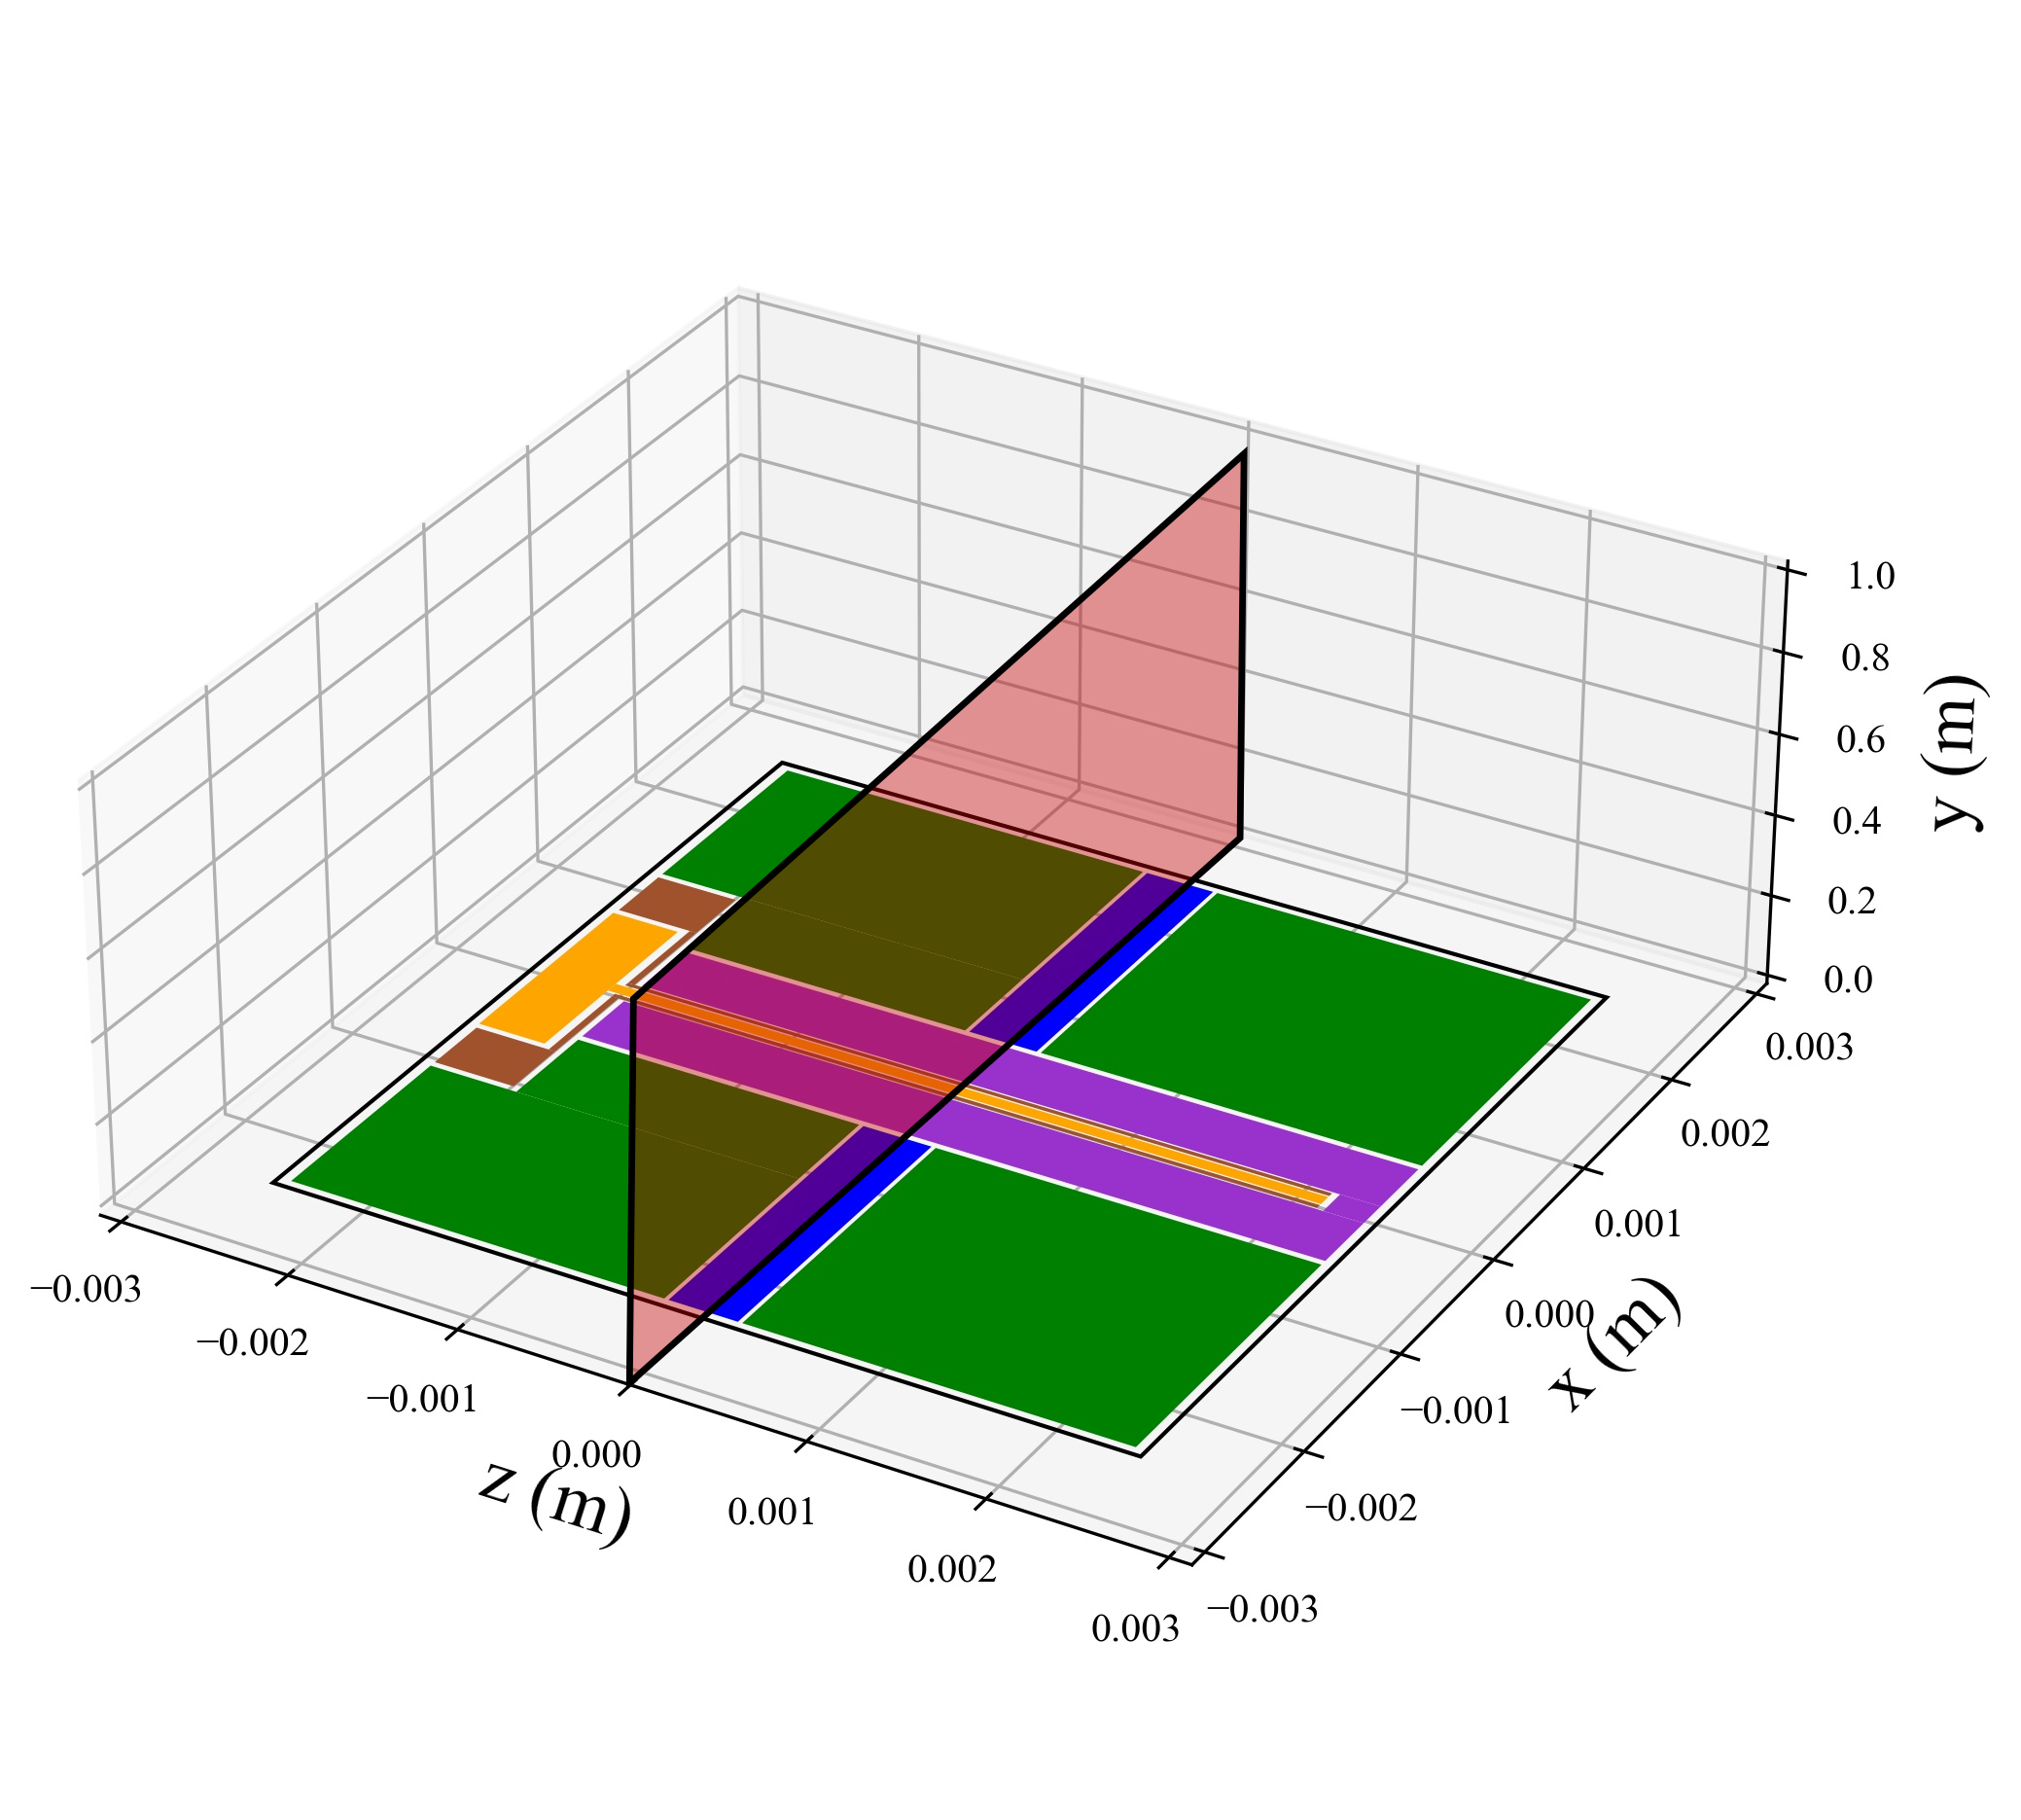
\includegraphics[width = 0.7\linewidth]{./simulation/figure/PlannarTrap_3D_z=0.png}
	\end{center}
\end{figure}
\begin{figure}[h]
	\begin{center}
		\begin{minipage}{0.45\linewidth}
			\begin{center}
				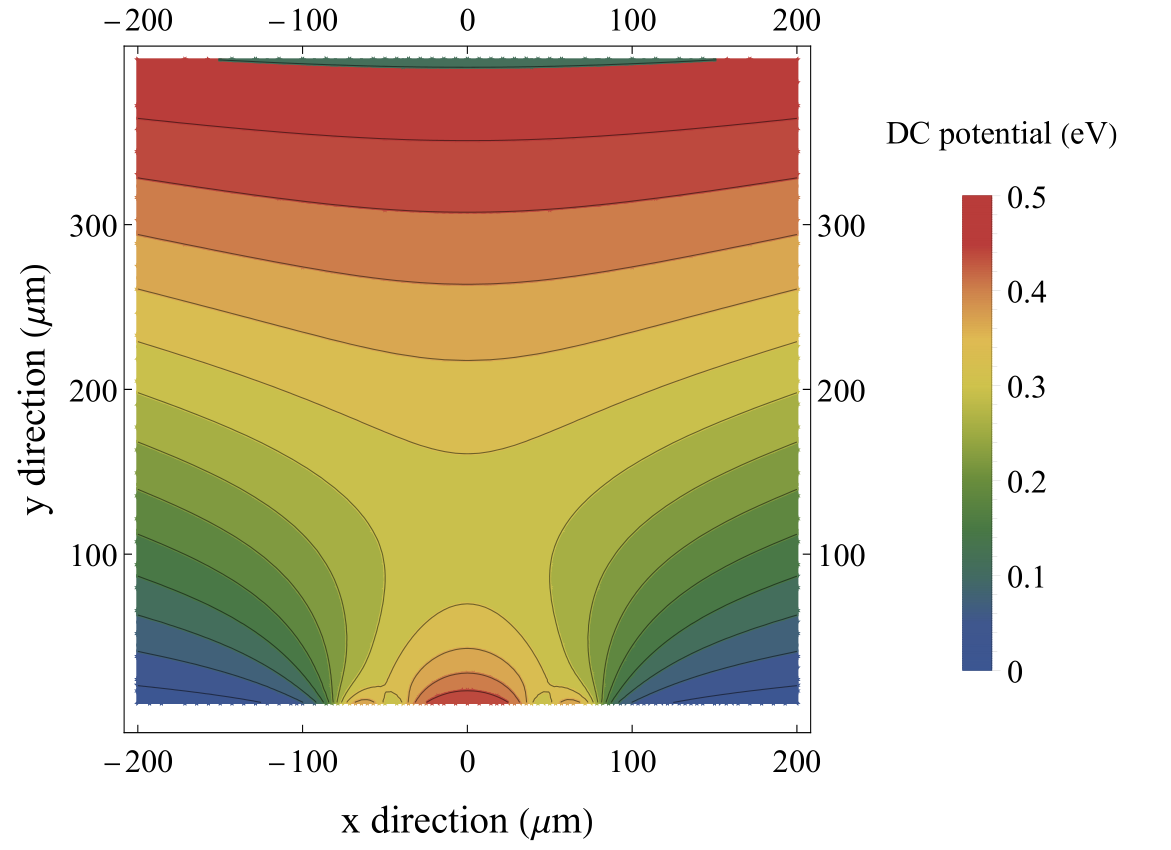
\includegraphics[width = 1.2\columnwidth]{./simulation/figure/dc_potential_example.png}
			\end{center}
		\end{minipage}
		\begin{minipage}{0.45\linewidth}
			\begin{center}
				\begin{tabular}{c|c} \hline \hline
					電極 & 印加電圧 ()V) \\ \hline
					End1 & 1.41 \\ \hline
					End2 & 1.41 \\ \hline
					End3 & 1.41 \\ \hline
					End4 & 1.41 \\ \hline
					Mid1 & -1.532 \\ \hline
					Mid2 & -1.532 \\ \hline
					Side1 & 0.222 \\ \hline
					Side2 & 0.222 \\ \hline
					center & 0.225 \\ \hline
				\end{tabular}
			\end{center}
		\end{minipage}
	\end{center}
\end{figure}
\section{Single-wellにおけるrf擬ポテンシャル}
\begin{figure}[h]
	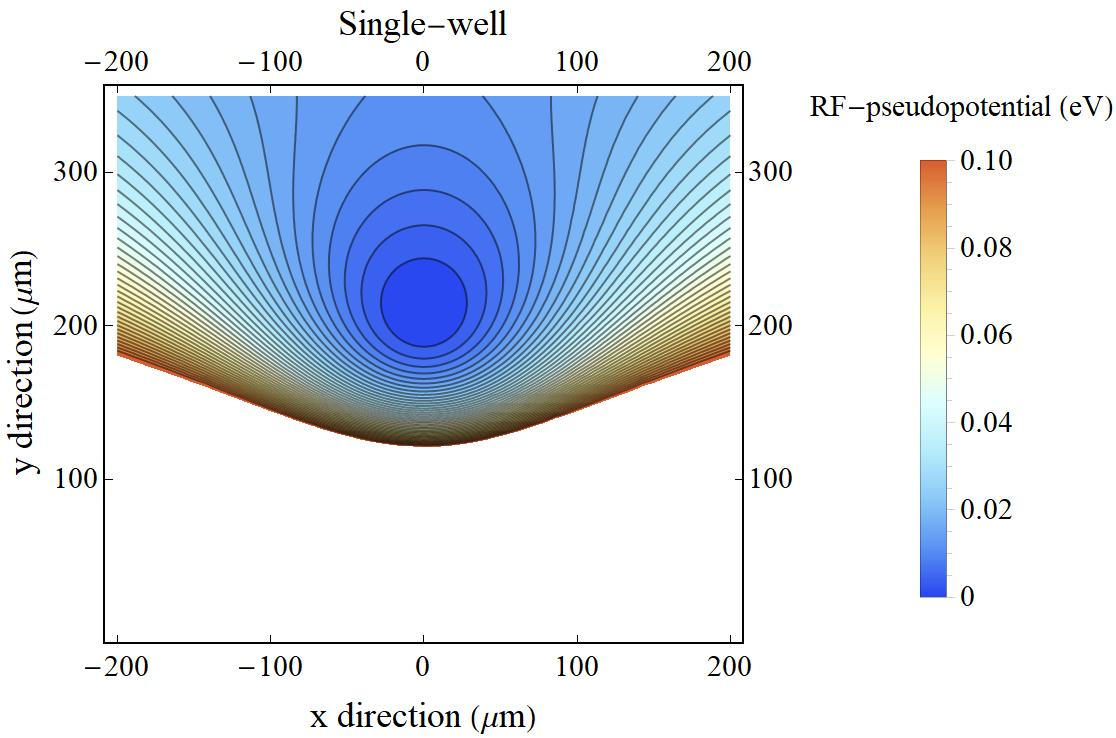
\includegraphics[width = 0.7\linewidth]{./simulation/figure/Single-well_Contour_xy@z=0.jpg}
	\caption{single-well}
	\label{fig:single-well_example}
\end{figure}
\section{Double-wellにおけるrf擬ポテンシャル}
\begin{figure}[h]
	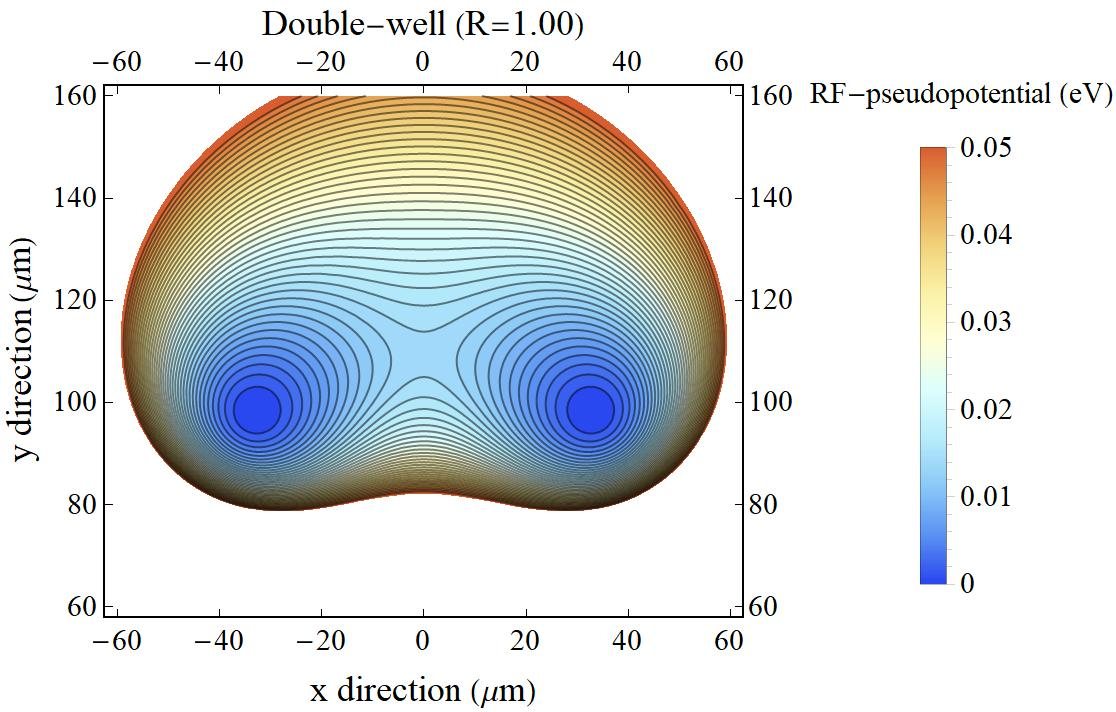
\includegraphics[width = 0.7\linewidth]{./simulation/figure/Double-well_Contour_xy_R=100.jpg}
	\caption{double-well}
	\label{fig:double-well_example}
\end{figure}
	% -- 実験方法 -- %
	\chapter{実験方法}
\section{一列配列イオンの捕獲}
\begin{enumerate}
\item まず,照射するレーザーのセットアップを行う.
\begin{enumerate}
\item 波長計(HighFinesse,MC-15)を起動させ,基準周波数としてHe-Neレーザを点ける.
\item 375-nm(THORLABS,LDC202C)の電源を点け,電流を65mAに設定する.
\item 397-nm(TOPICA PHOTONICS,DCC110)のmoduleをonにし,CURRENT CTRをonにする.調節ねじを4に回し,電流を51mA付近に設定する.
\item 866-nm(Newport, $R_{\rm SET} = 11.682 {\rm k}\Omega , I_{0} = 145.16{\rm mA}$)をENABLEに設定する.
\item arroyo instruments, ComboPak,685-0.1を使用して,423-nmのECDLに電流を60.04mAを流し,温度を26.550C$^{\circ}$に設定する.
\item \Tb{use_laser_wavelength}にイオン捕獲を行ったときの波長を示す.

\begin{table}[h]
	\centering
		\caption{$^{40}{\rm Ca}^+$捕獲時に使用するレーザーの波長}
		\label{tab:use_laser_wavelength}
		\begin{tabular}{c}\hline \hline
			632.99050 nm \\
			866.45120 nm \\
			396.95890 nm \\
			422.79157 nm \\ \hline
		\end{tabular}
\end{table}

\item プレーナートラップ上のイオン捕獲位置でレーザーの焦点が合うように真空チャンバーの手前にレンズを設置しており,マイクロメーターを用いて上下左右に移動させることができる.一列配列イオンでは\Fig{lens_string}で示されるイオンが並ぶ方向に対して垂直に照射するレーザーのマイクロメータの目盛が鉛直方向に4,水平方向に39であり,斜めに照射するレーザーのマイクロメータの目盛は鉛直方向が10,水平方向は0である.

 \begin{figure}[h] 
 	\begin{center}
 		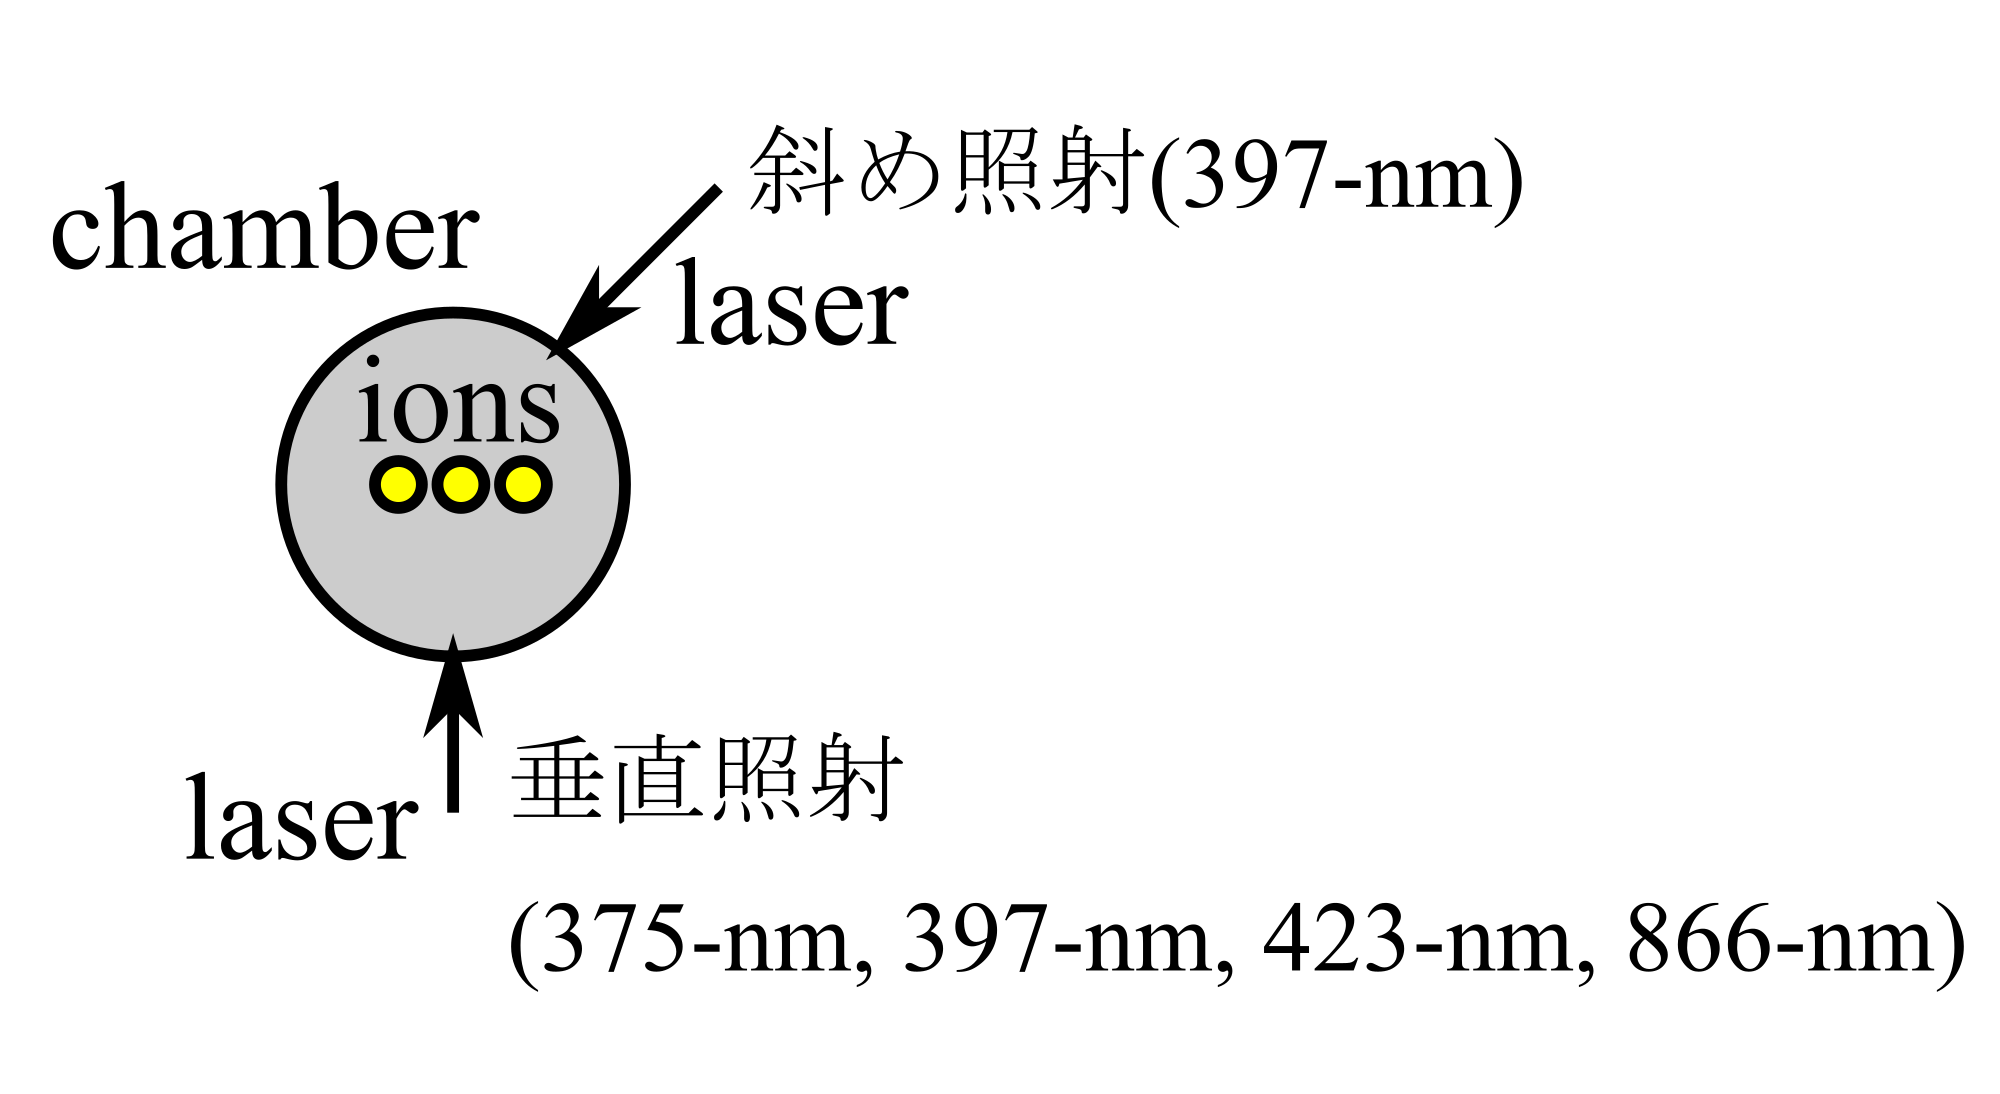
\includegraphics[scale=0.4]{./methods/figure/in_laser.png}
 		\caption{プレーナートラップに照射する二本のレーザー}
 		\label{fig:lens_string}
 	\end{center}
 \end{figure}
\end{enumerate}

\clearpage

\item 次にプレーナートラップに印加するdc電圧とrf電圧のセットアップを行う.
\begin{enumerate}
\item プレーナートラップの各電極に\Tb{dc_string}に示すdc電圧を印加する.

\begin{table}[h]
	\centering
		\caption{一列配列イオンを捕獲するためにプレーナートラップに印加するdc電圧セット}
		\label{tab:dc_string}
		\begin{tabular}{c|c} \hline \hline
			dc電極 & dc電圧 \\ \hline
			End1 & 1.44  V \\
			End2 & 1.406  V \\
			End3 & 1.44  V \\
			End4 & 1.406 V \\
			center & 0.225 V \\
			side1 & 0.222 V \\
			side2 & 0.222 V \\
			middle1 & -1.532 V \\
			middle2 & -1.532 V \\ \hline
		\end{tabular}
\end{table}

\item 発振器(KEYSIGHT,33500B Series)を用いてrf信号を発生させる.周波数は27.2 MHzで,rf電極に印加される信号には320mV$_{\rm pp}$(CH1),center-rf電極に印加される信号には1mV$_{\rm pp}$(CH2)を設定し,増幅器(R\&K,A000110-4040-R)を利用して,増幅されたrf信号をプレーナートラップに印加する.rf電圧の波形を\Fig{1D_wave}に示す.

\begin{figure}[h]
	\begin{minipage}{0.48\linewidth}
		\begin{center}
			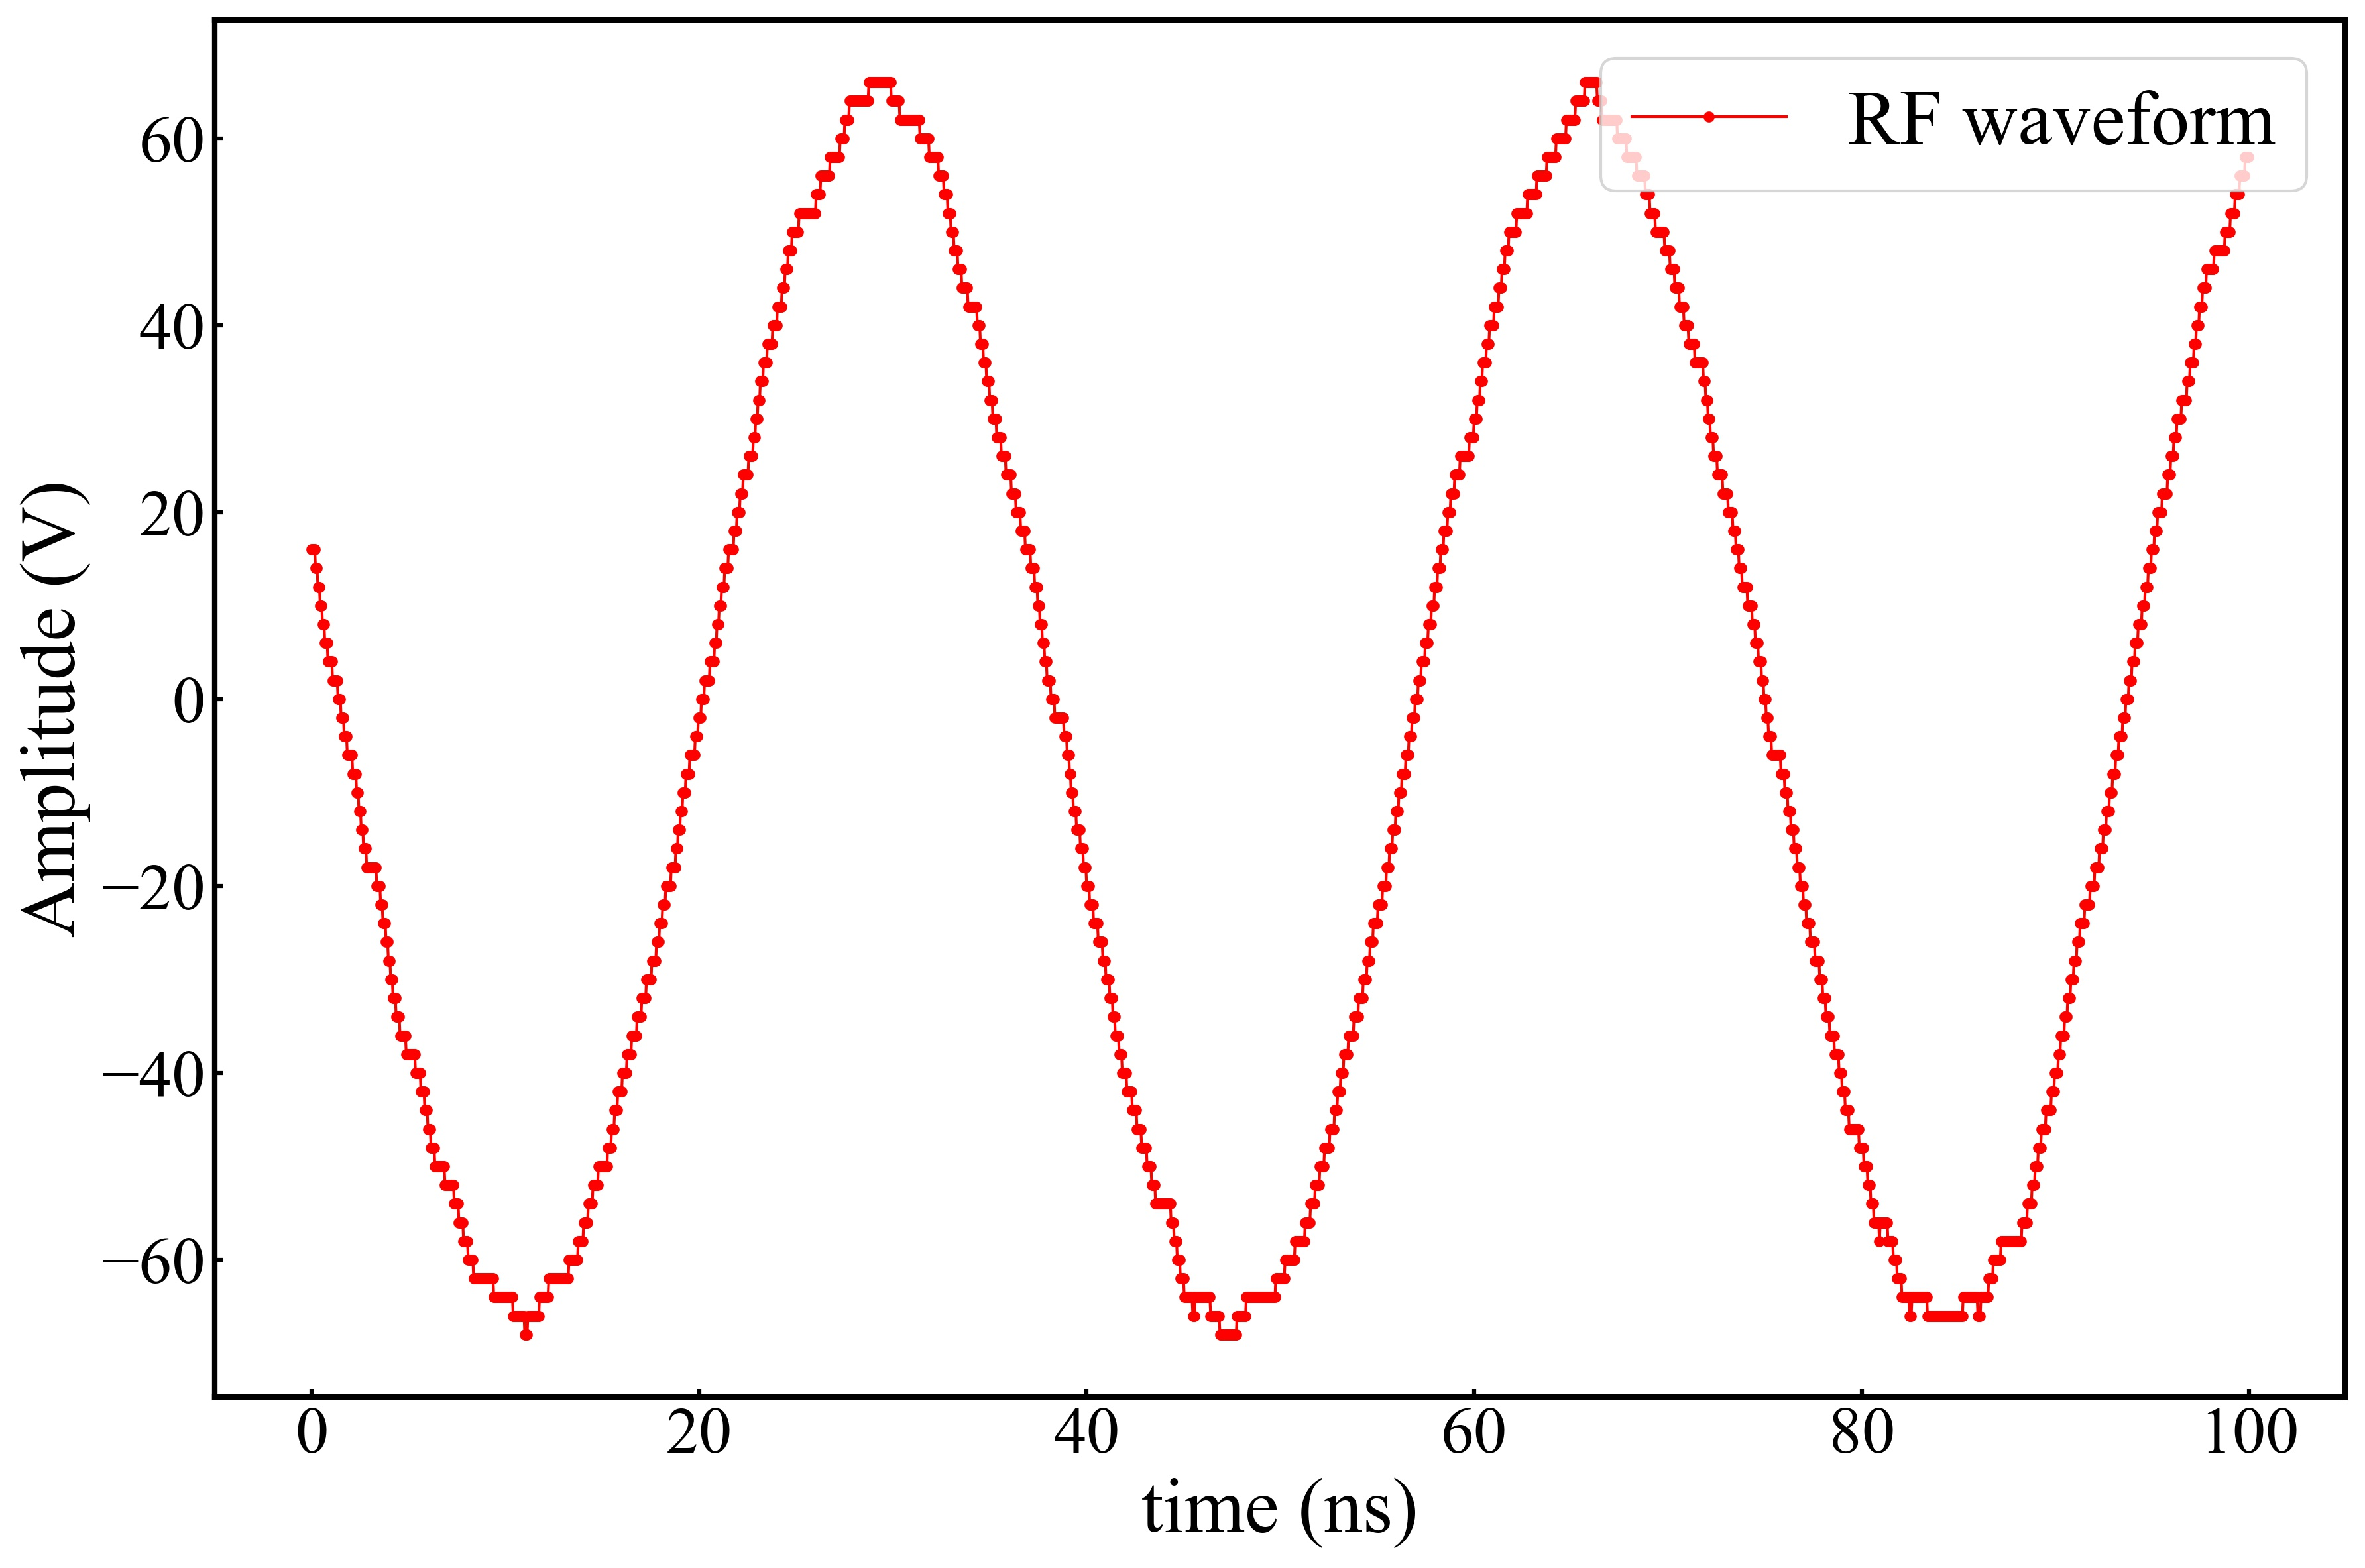
\includegraphics[width=0.9\columnwidth]{./methods/figure/1D_wave.jpg}
			\caption{一列配列イオンを捕獲するために使用するrf電圧の波形}
			\label{fig:1D_wave}
		\end{center}
	\end{minipage}
	\begin{minipage}{0.48\linewidth}
		\begin{center}
			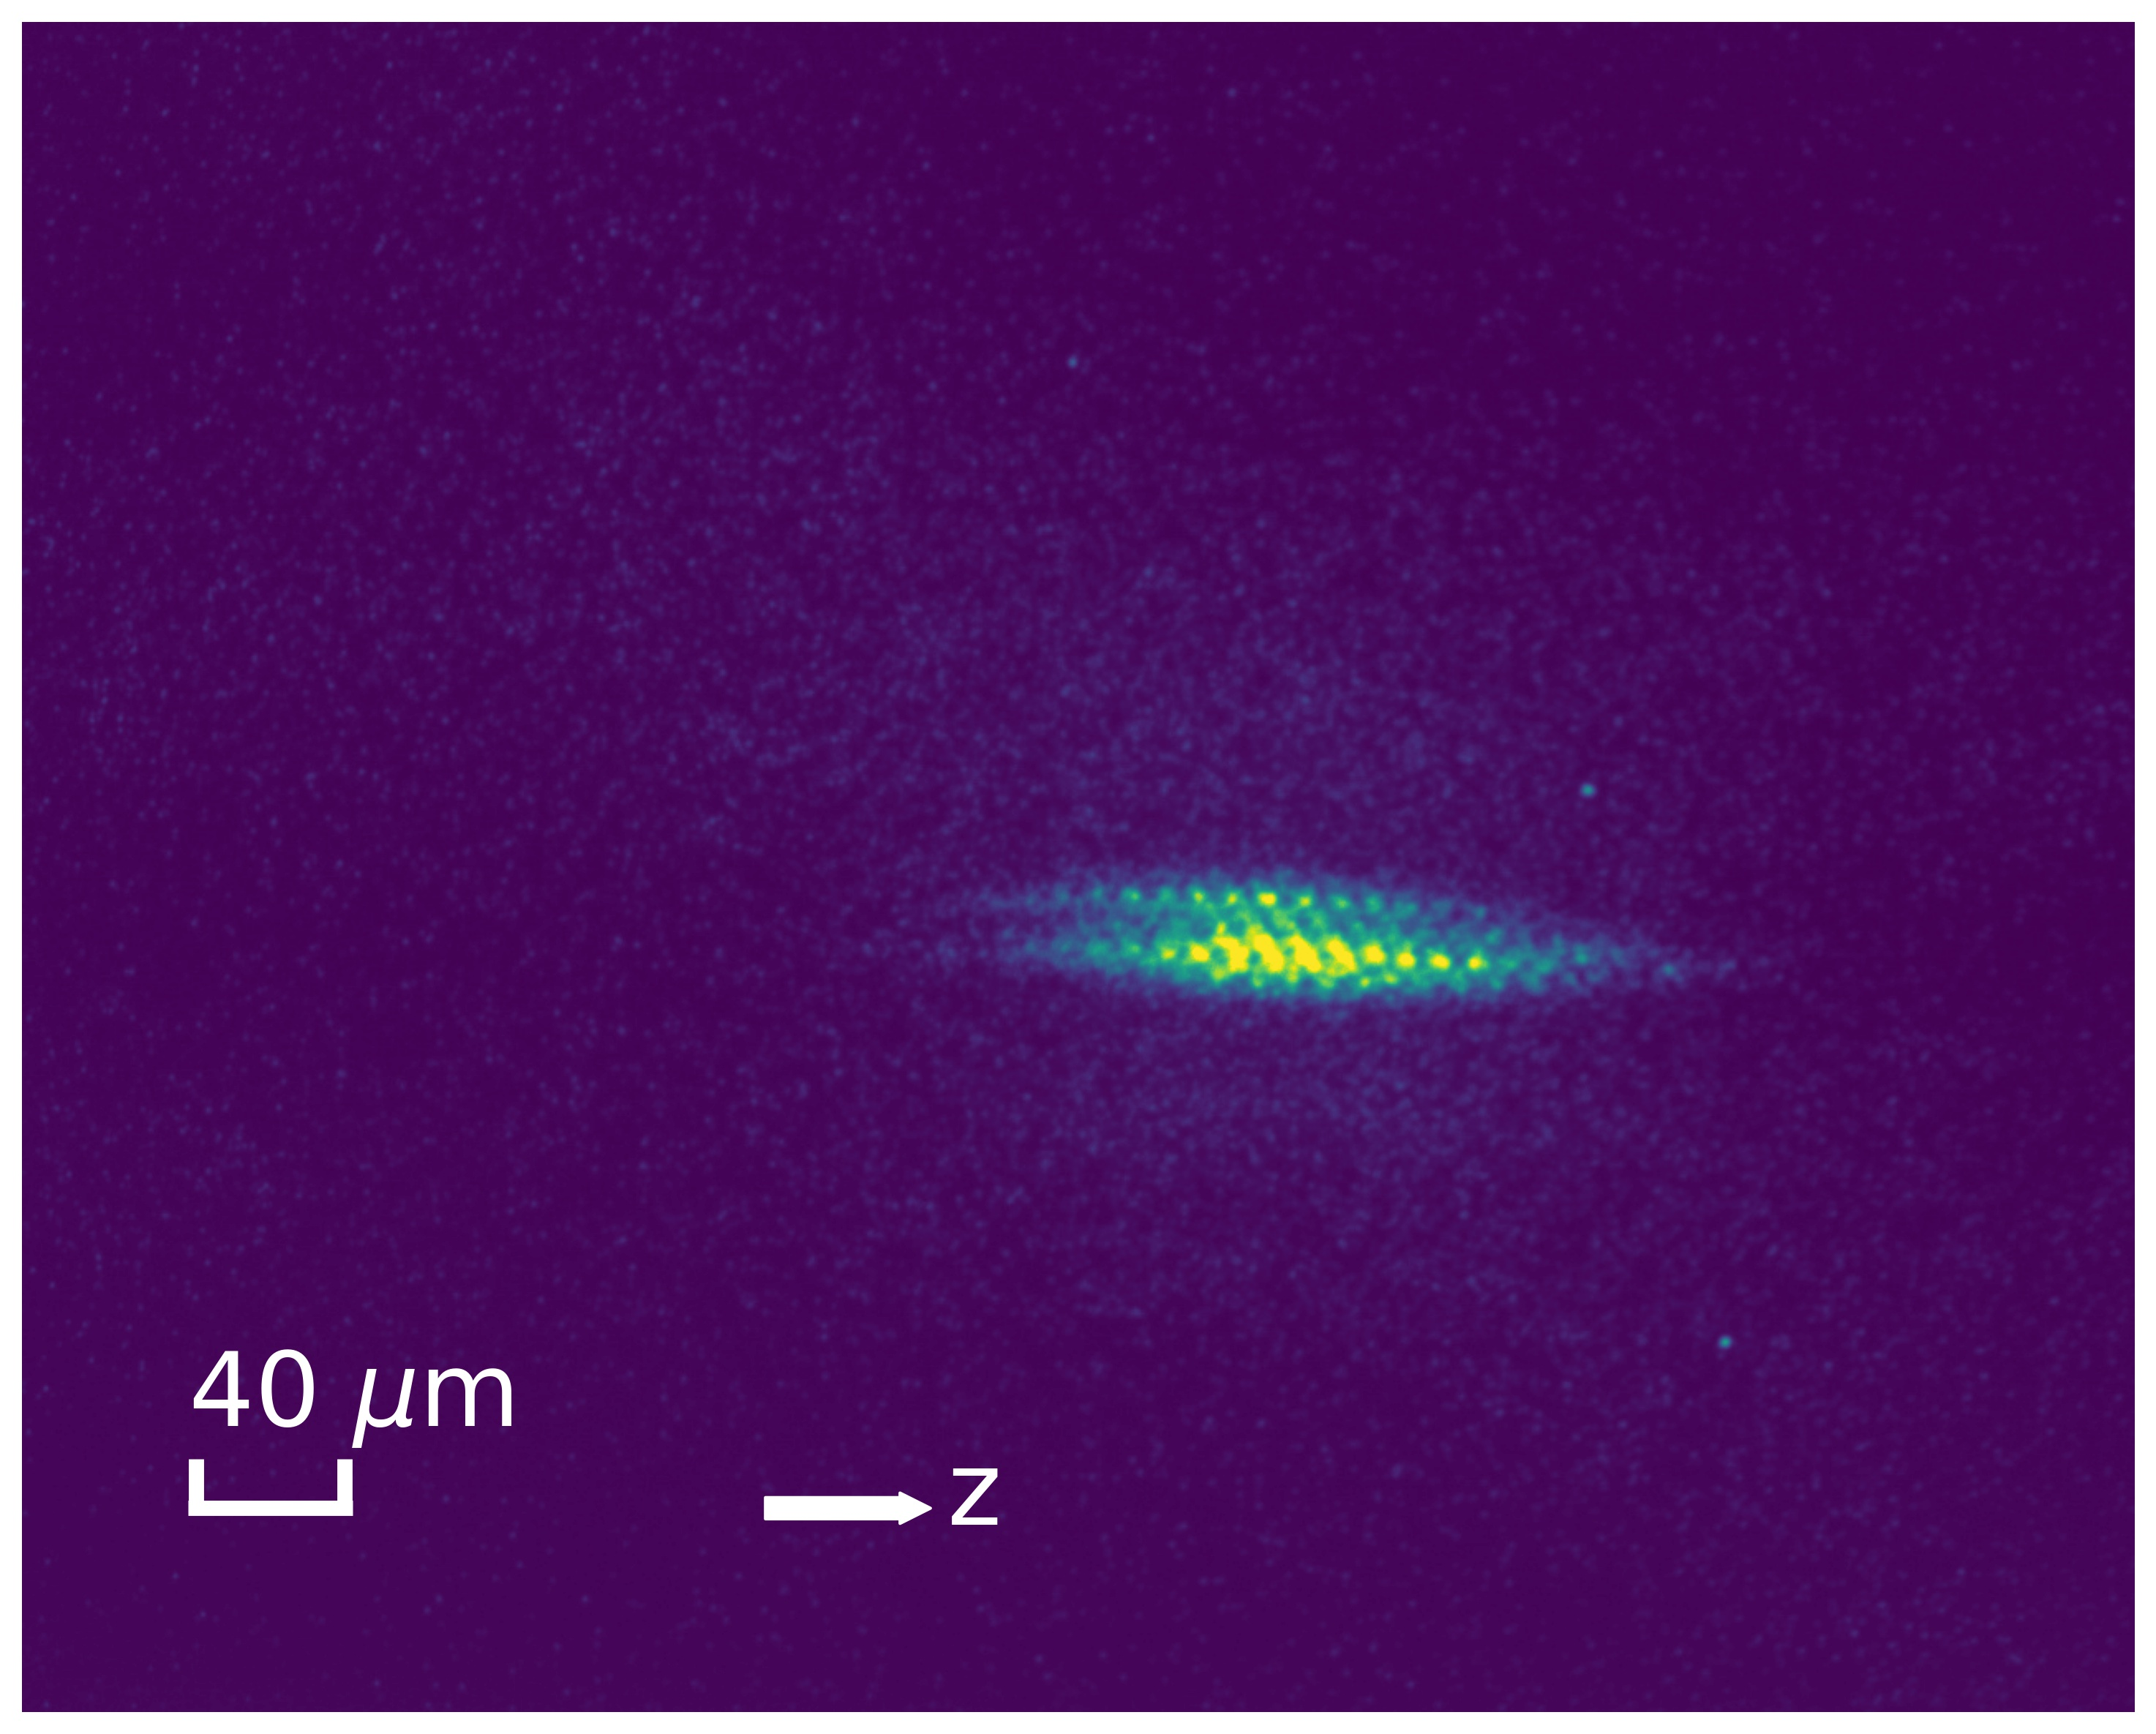
\includegraphics[width=0.6\columnwidth]{./methods/figure/string.jpg}
			\caption{4分間オーブンによる加熱を行ったあとのイオン捕獲画像(真空度:$2.85 \times 10^{-10}$Torr)}
			\label{fig:Cap_string}
		\end{center}
	\end{minipage}
\end{figure}

\item 磁場の印加(TPO7-5)を行い,カルシウム原子を射出させるために加熱を行うオーブンの電源を点ける.

\item Image Intensifier(HAMAMATSU,
 C9016-02)と汎用CCDカメラ(THORLABS,DCC3420M)を組み合わせた検出系でイオンの蛍光を集光する.電源を点け,露光時間は10ms,Gainは4.0に設定する.
 
\item オーブンをLabVIEWを介して制御し,適宜レーザーの波長を調節しながらイオンが捕獲されるまでオーブンによる加熱を続ける.

\item 4分間オーブンによる加熱を行ったときのイオン捕獲画像を\Fig{Cap_string}に示している.
\end{enumerate}
\end{enumerate}
%
\clearpage
%
\section{二列配列イオンの捕獲}
二列配列イオンの捕獲手順を説明する.一列配列イオンの捕獲条件との主な変更点は
\begin{itemize}
	\item center-RF信号の振幅
	\item イオン捕獲位置の変化によるレーザー照射位置の調整と集光系のピントの調整
	\item dc電圧の調整
\end{itemize}
の3つである.以下,二列配列イオンの捕獲手順を示す.\\
\begin{enumerate}
\item まずは,一列配列イオンの捕獲条件で多数のイオンの捕獲を行う.\Fig{1_2D}にこのときのイオン捕獲画像,\Fig{1_2D_wave}にオシロスコープで取得したrf電圧とcenter-rf電圧の関係を示す.rf電圧とcenter-rf電圧は発振器で発生させており,発振器上での出力設定はrf電圧の振幅が320mVpp,位相が0$^{\circ}$,center-rf電圧の振幅が1mVpp,位相が-40$^{\circ}$となっており,\Fig{1_2D_wave}は発振器から出力される信号が増幅されトラップに印加される直前の点で計測を行っている.

\begin{figure}[h]
	\begin{minipage}{0.48\linewidth}
	\begin{center}
		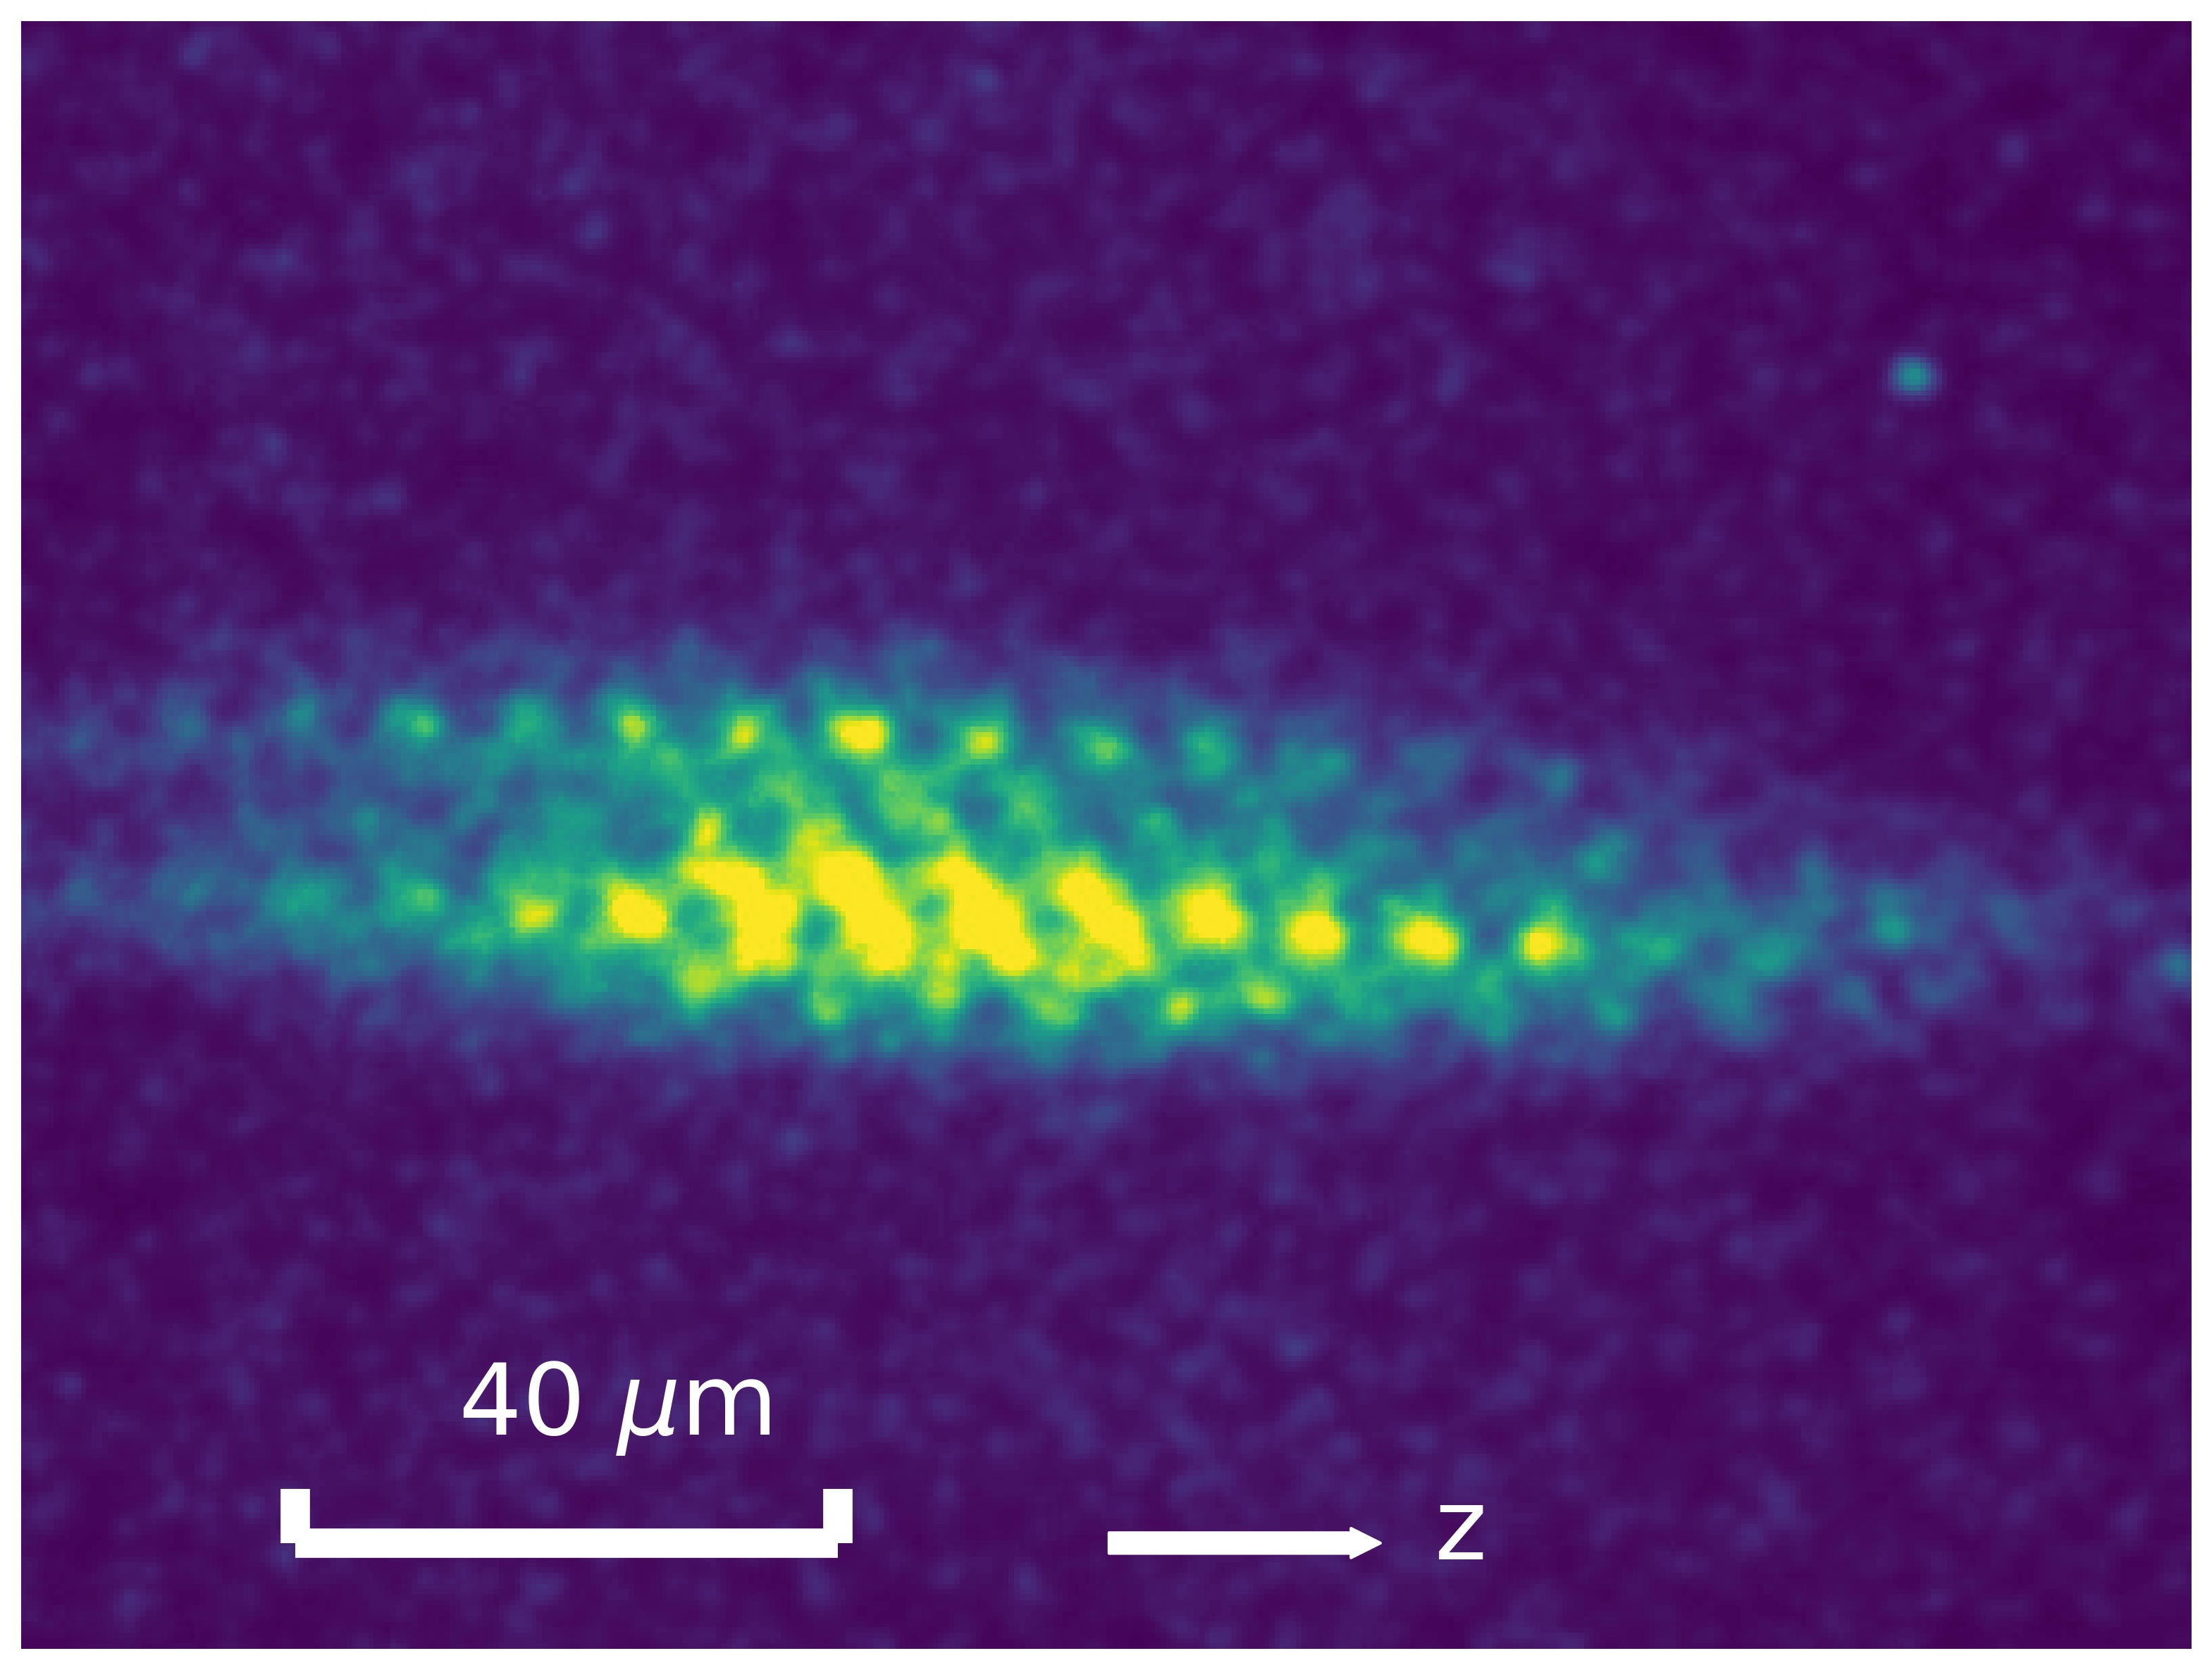
\includegraphics[width = 0.6\columnwidth]{./methods/figure/1_2D.jpg}
		\caption{手順1でのイオン捕獲画像}
		\label{fig:1_2D}
	\end{center}
	\end{minipage}
	\begin{minipage}{0.48\linewidth}
		\begin{center}
			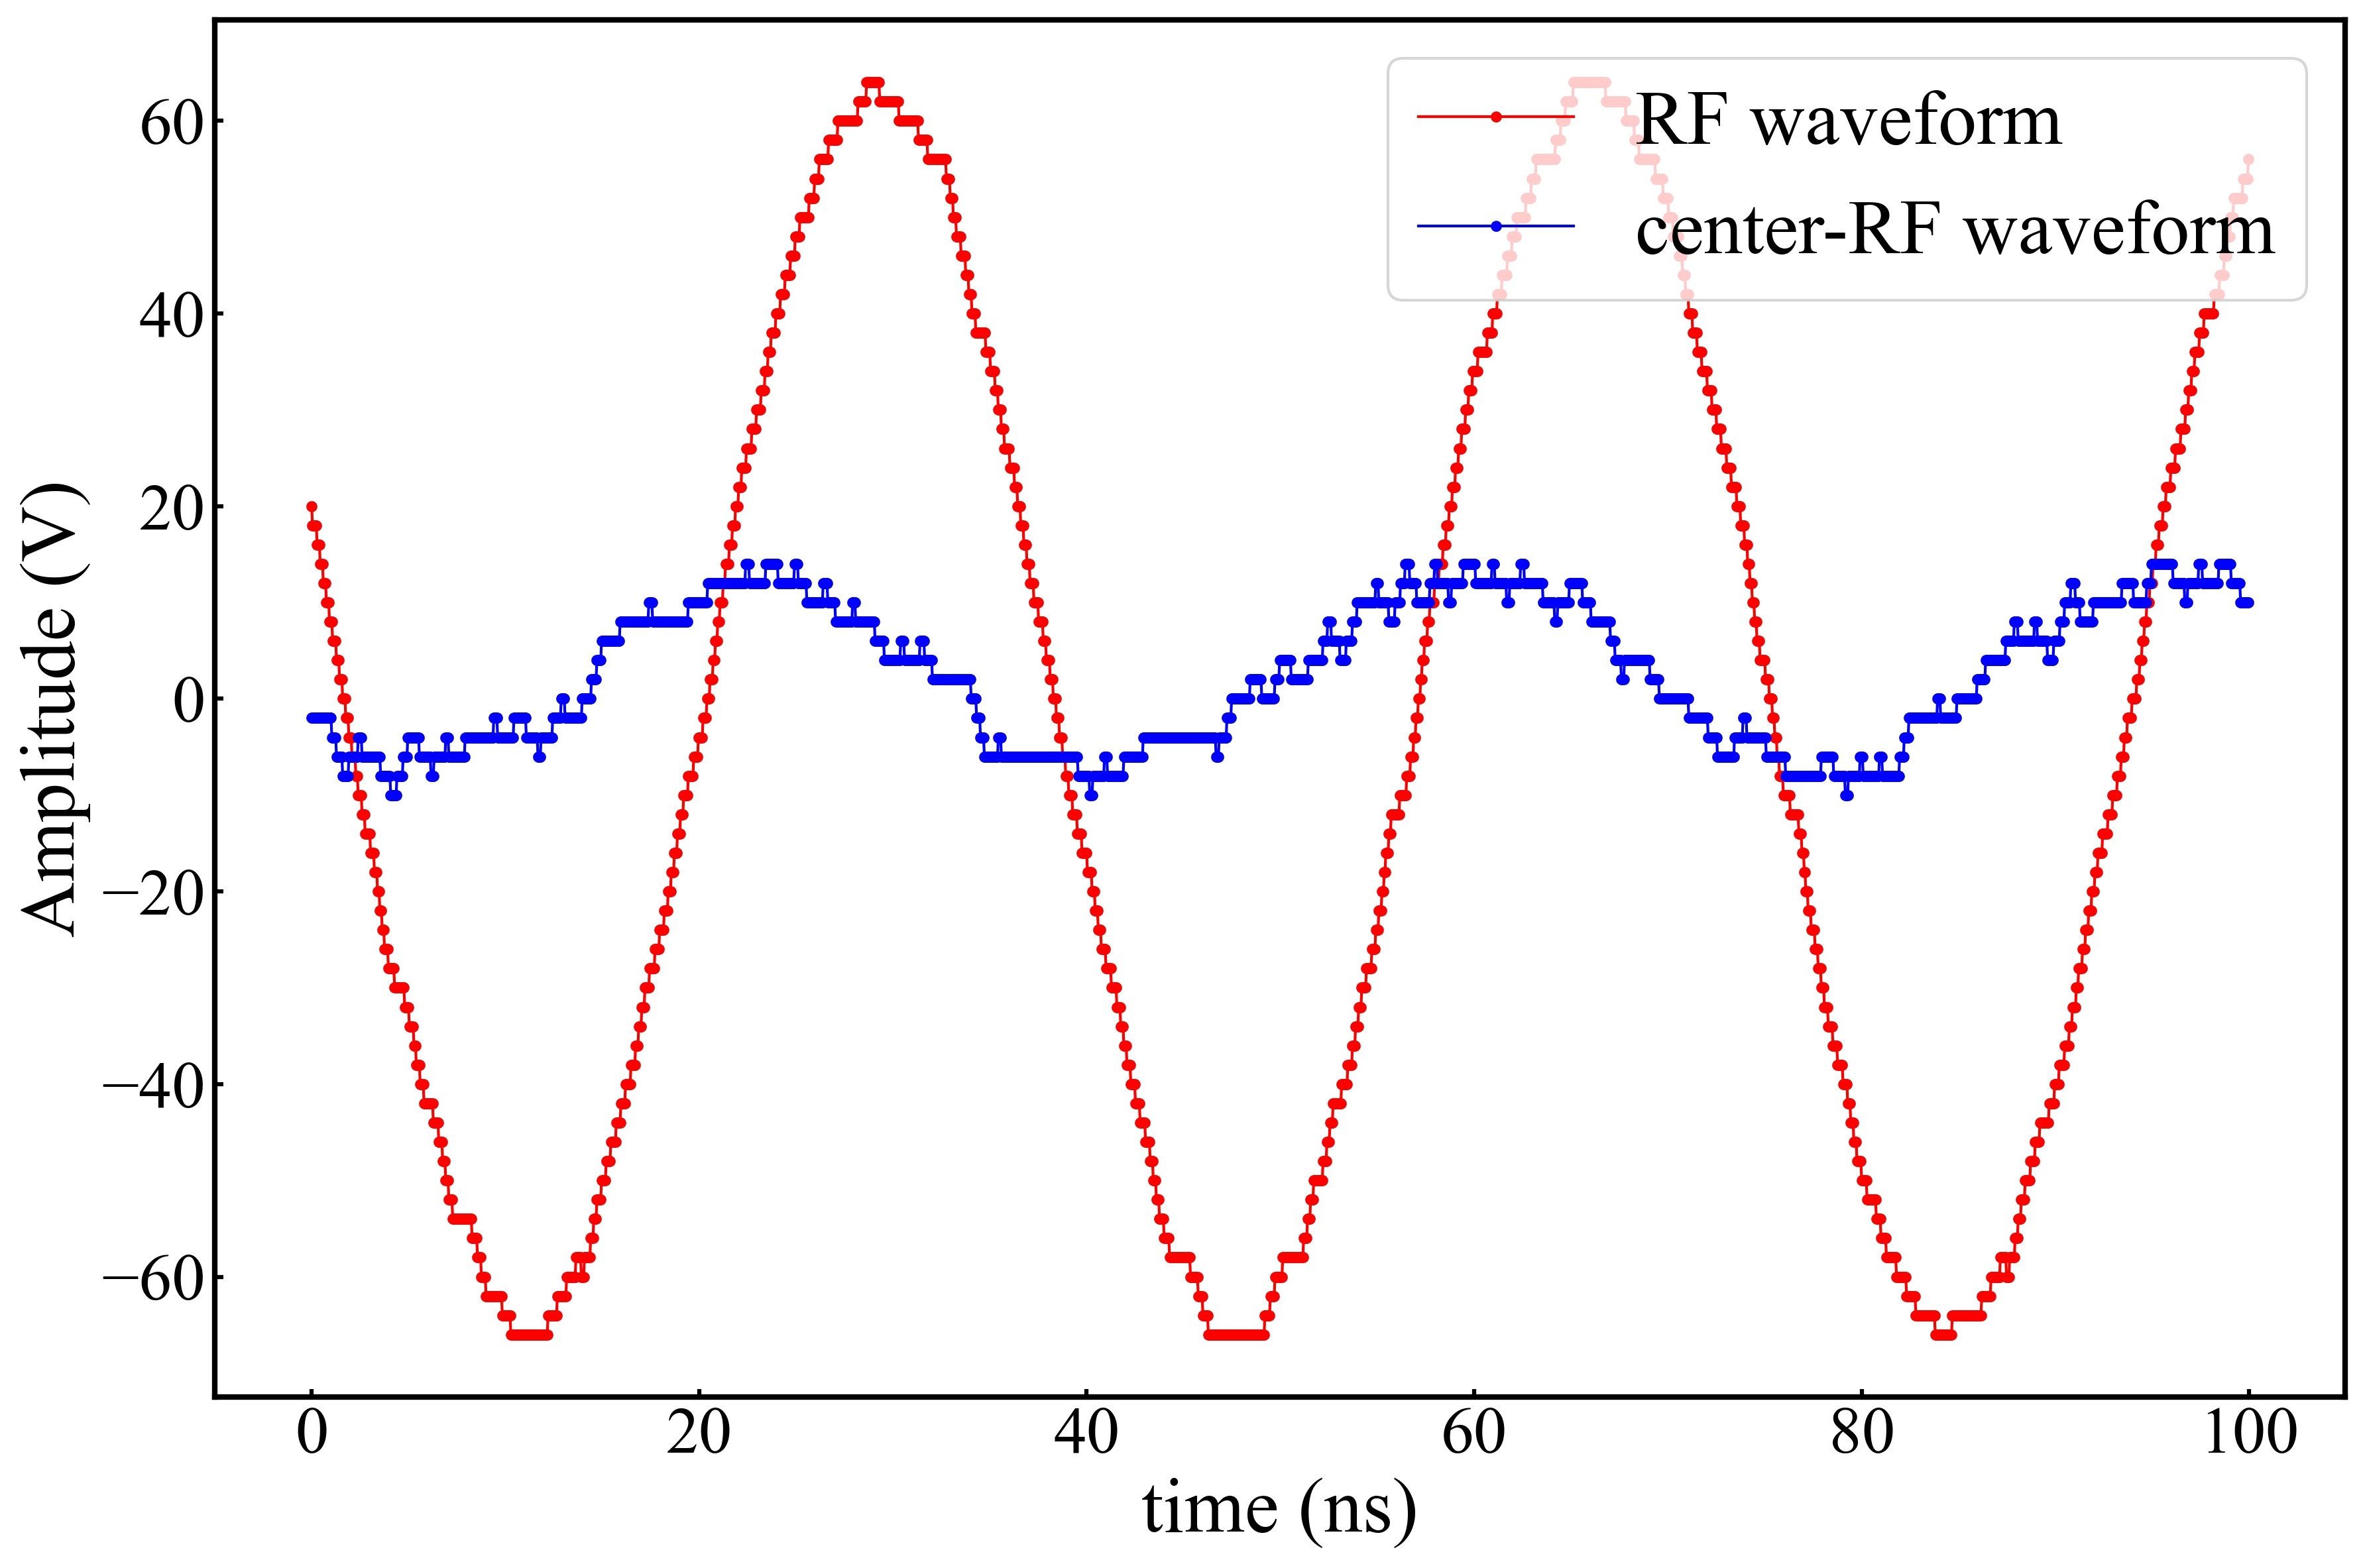
\includegraphics[width = 0.9\columnwidth]{./methods/figure/1_2D_wave.jpg}
			\caption{手順1におけるrf電圧とcenter-rf電圧の関係}
			\label{fig:1_2D_wave}
		\end{center}
	\end{minipage}
\end{figure}

これより,$R=0.21$となっている.また,各レーザーの焦点を絞るためのレンズの位置を調節するマイクロメータの目盛を\Tb{1_2D}に示す.

\begin{table}[h]
	\begin{center}
	\caption{手順1におけるレンズの位置を調節するマイクロメータの目盛}
	\label{tab:1_2D}
	\begin{tabular}{c|cc} \hline \hline
		&鉛直方向&水平方向 \\ \hline
		垂直照射&39 & 4 \\ 
		斜め照射&10 & 0 \\ \hline
	\end{tabular}
	\end{center}
\end{table}

\item 次に,center-rf電圧の振幅を発振器上で100mVppに設定する.1.と同様に\Fig{2_2D}にイオン捕獲画像,\Fig{2_2D_wave}にrf電圧とcenter-rf電圧の関係を示す.\\
%
\clearpage
%
\begin{figure}[h]
	\begin{minipage}{0.48\linewidth}
	\begin{center}
		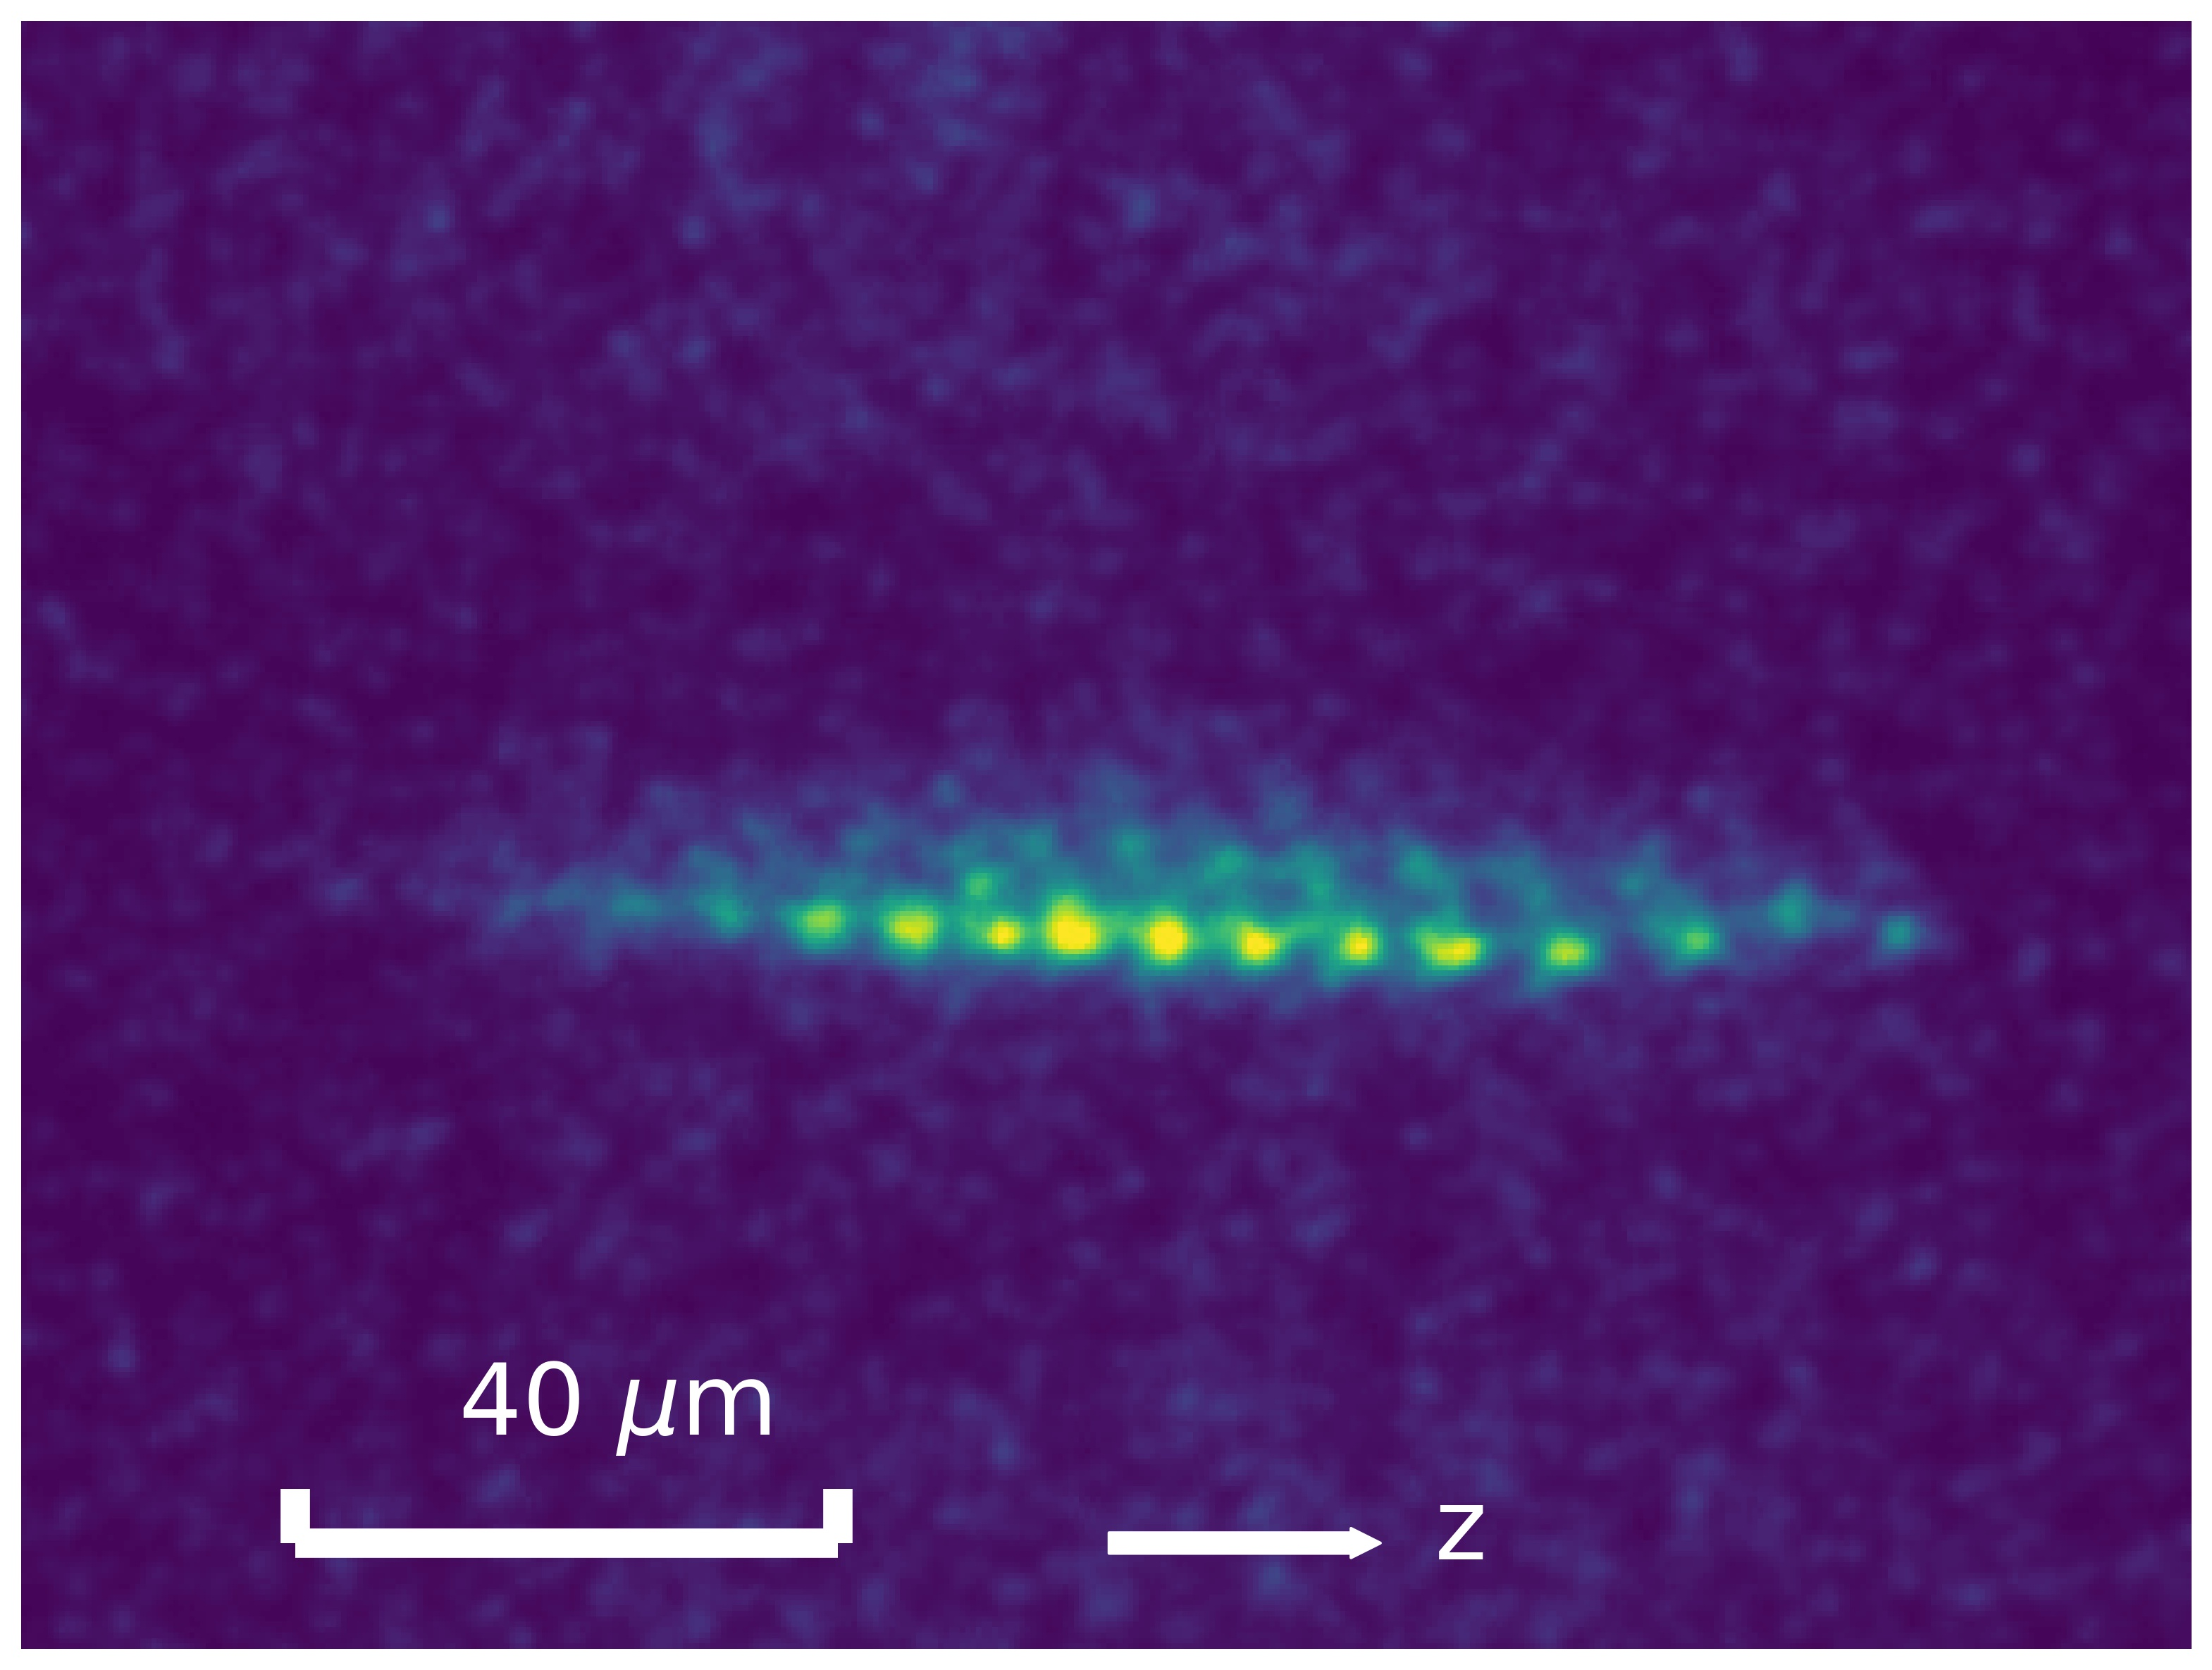
\includegraphics[width = 0.6\columnwidth]{./methods/figure/2_2D.jpg}
		\caption{手順2でのイオン捕獲画像}
		\label{fig:2_2D}
	\end{center}
	\end{minipage}
	\begin{minipage}{0.48\linewidth}
		\begin{center}
			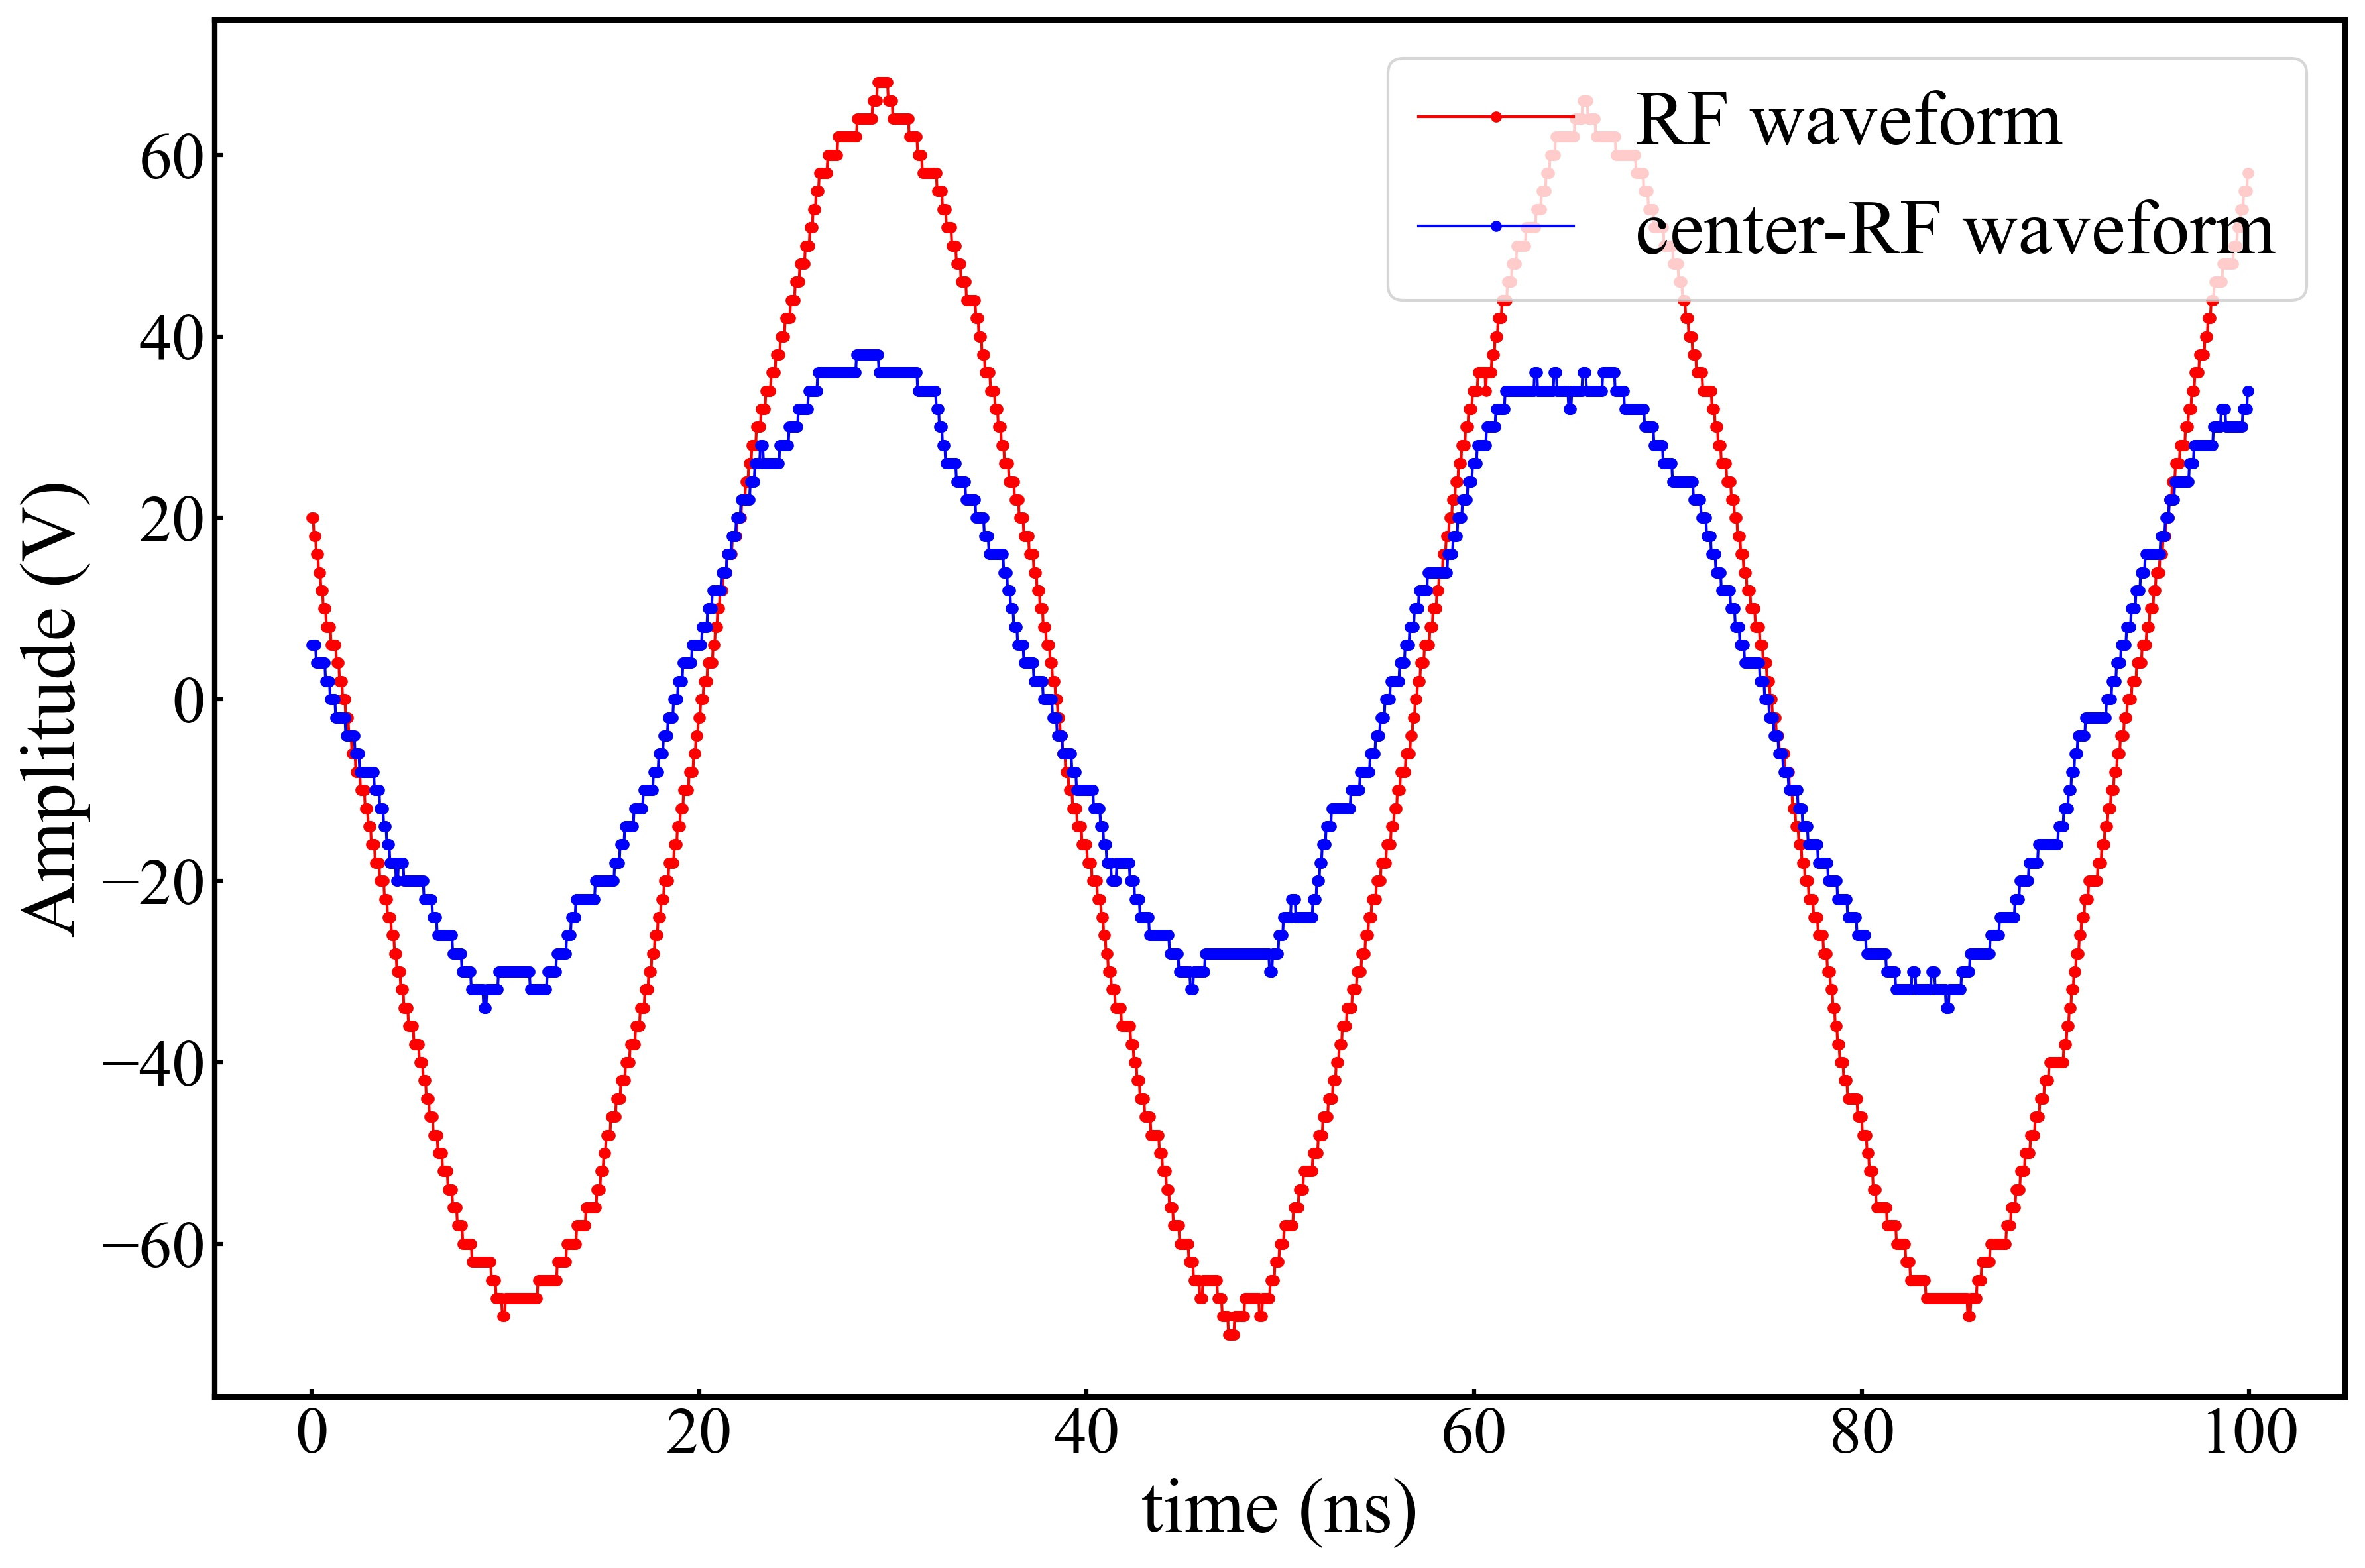
\includegraphics[width = 0.9\columnwidth]{./methods/figure/2_2D_wave.jpg}
			\caption{手順2におけるrf電圧とcenter-rf電圧の関係}
			\label{fig:2_2D_wave}
		\end{center}
	\end{minipage}
\end{figure}

これより,$R=0.56$である.マイクロメータの目盛を\Tb{2_2D}に示す.

\begin{table}[h]
\begin{center}
	\caption{手順2におけるレンズの位置を調節するマイクロメータの目盛}
	\label{tab:2_2D}
	\begin{tabular}{c|cc} \hline \hline
		&鉛直方向&水平方向 \\ \hline
		垂直照射&43 & 1 \\ 
		斜め照射&15 & 3 \\ \hline
	\end{tabular}
\end{center}
\end{table}

イオン捕獲位置がプレーナートラップ表面に近づき,レンズの位置がそれぞれ鉛直方向について下がることから,イオンの蛍光がはっきりと観測されるようにピントの調節を行っている.
\item 発振器上でcenter-rf電圧を135mVppに設定する.\Fig{3_2D}にイオン捕獲画像,\Fig{3_2D_wave}にrf電圧とcenter-rf電圧の関係を示す.

\begin{figure}[h]
	\begin{minipage}{0.48\linewidth}
	\begin{center}
		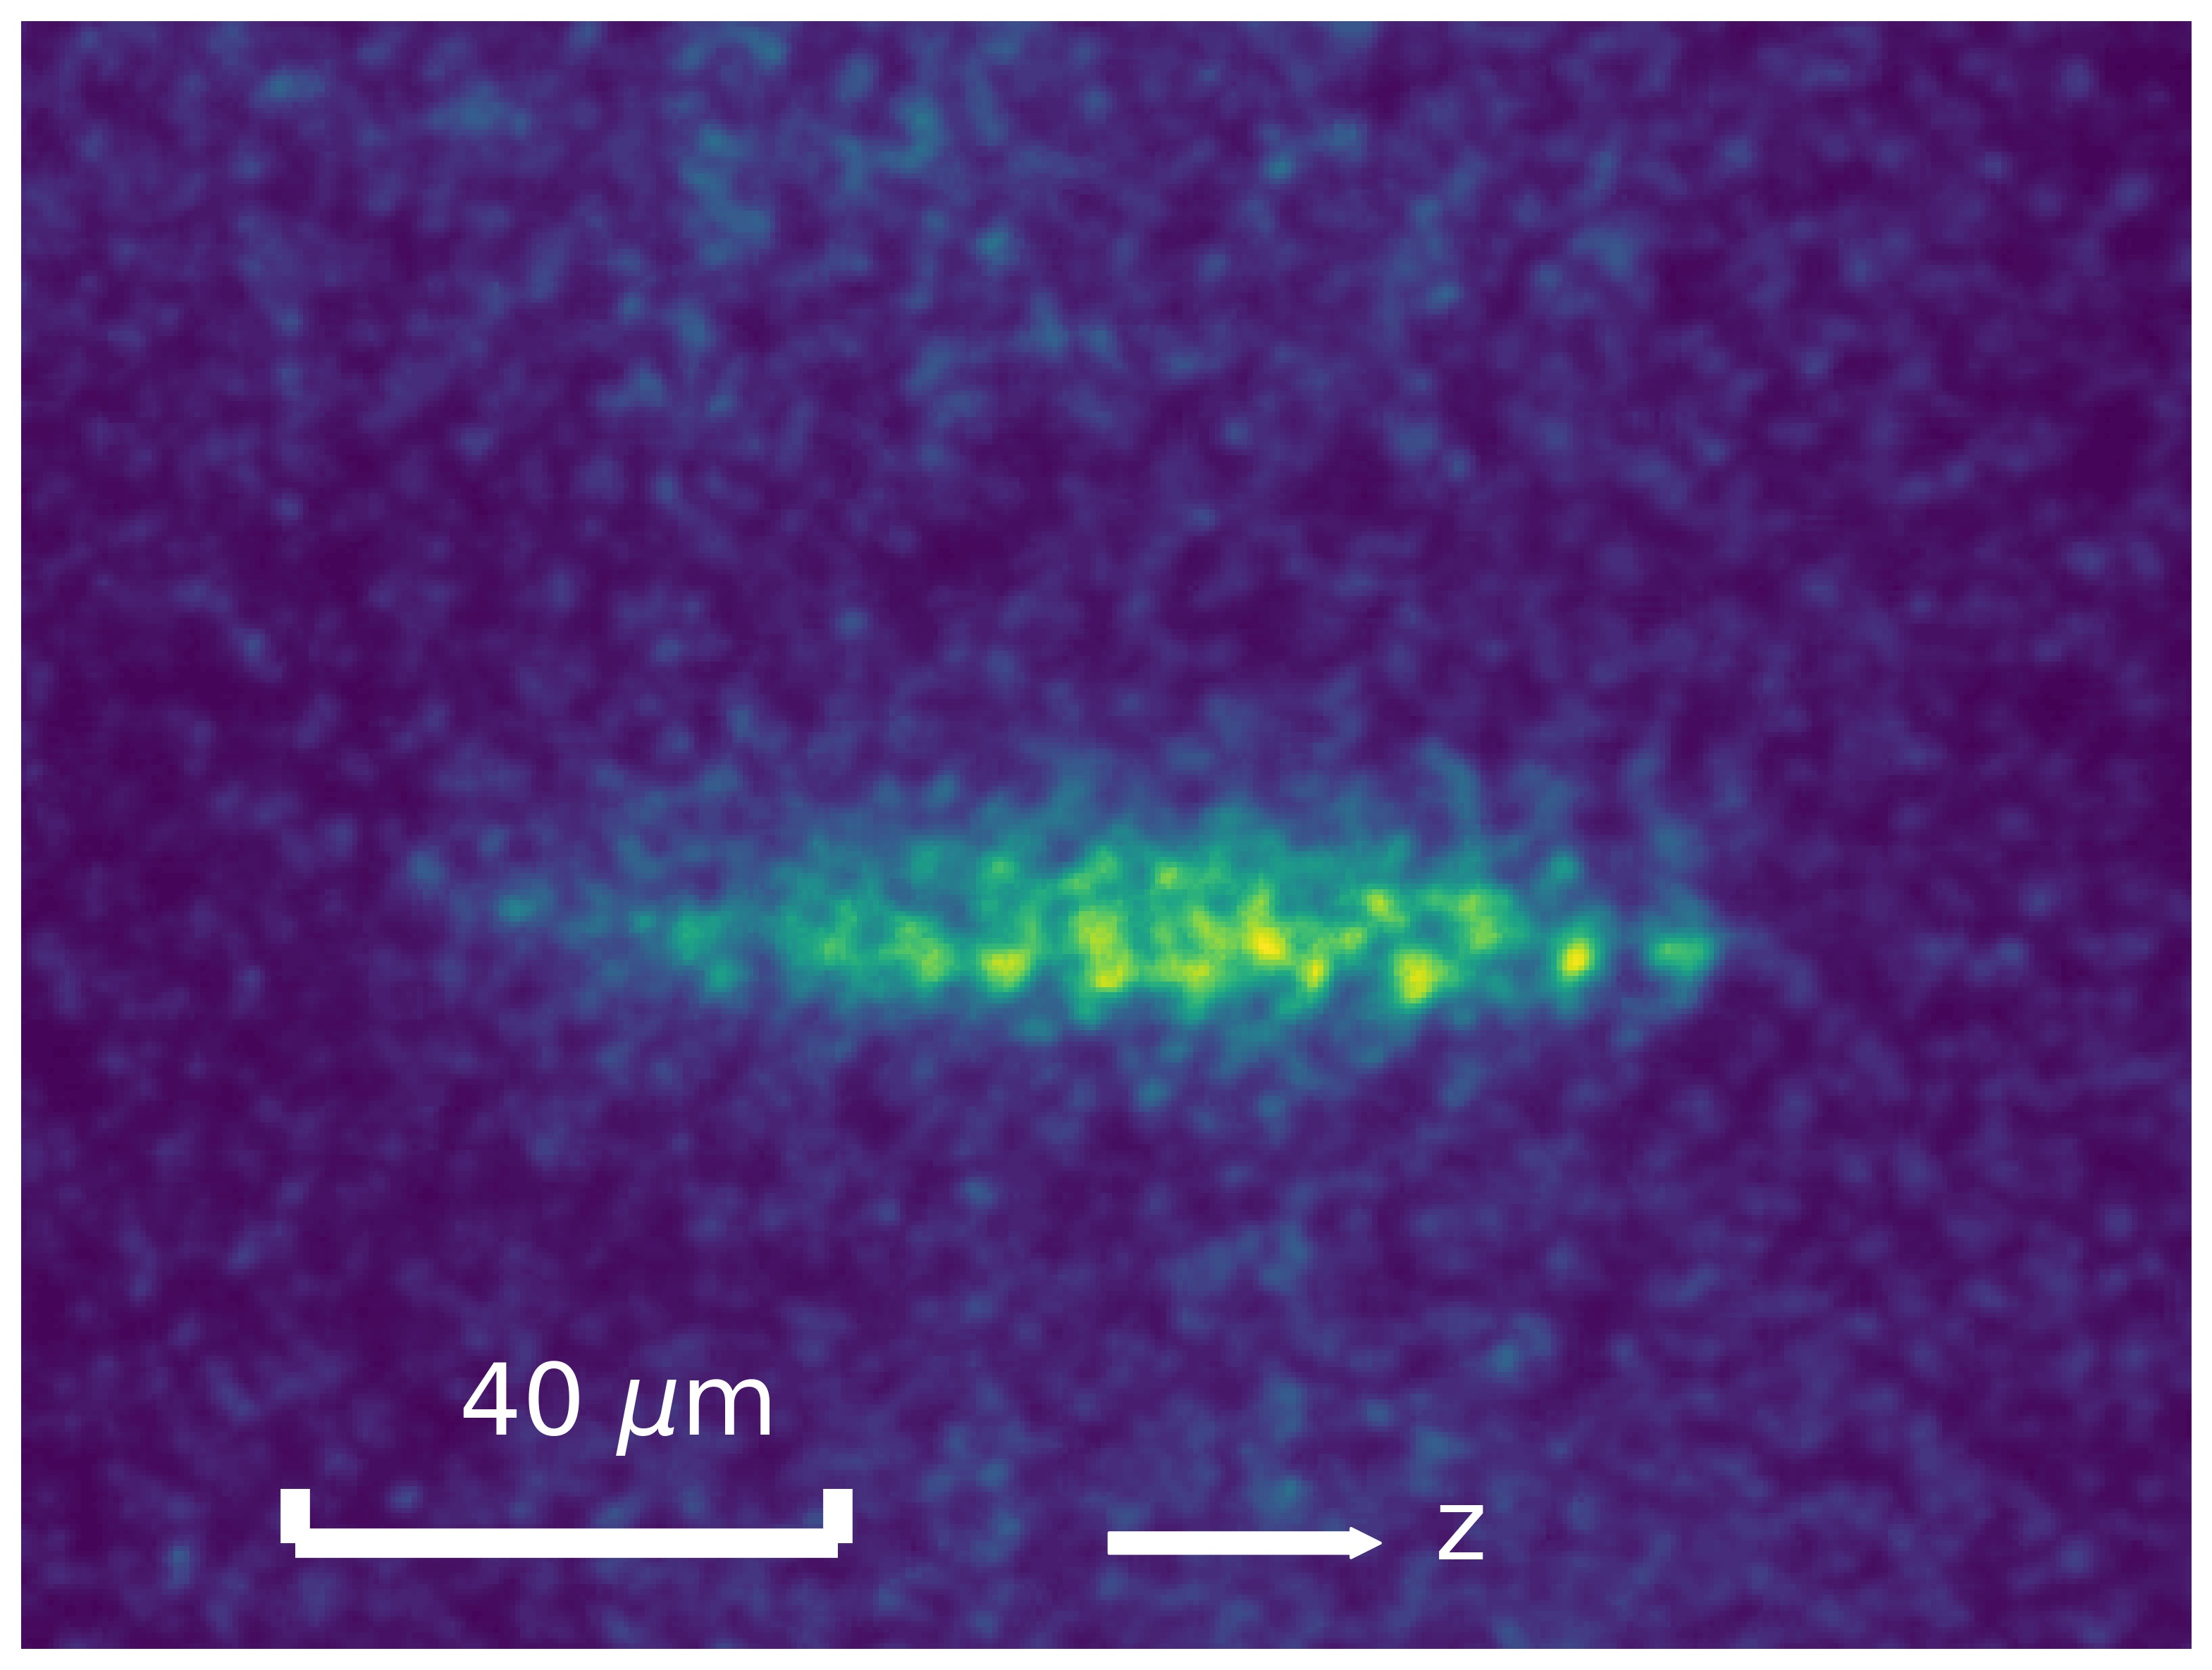
\includegraphics[width = 0.6\columnwidth]{./methods/figure/3_2D.jpg}
		\caption{手順3でのイオン捕獲画像}
		\label{fig:3_2D}
	\end{center}
	\end{minipage}
	\begin{minipage}{0.48\linewidth}
		\begin{center}
			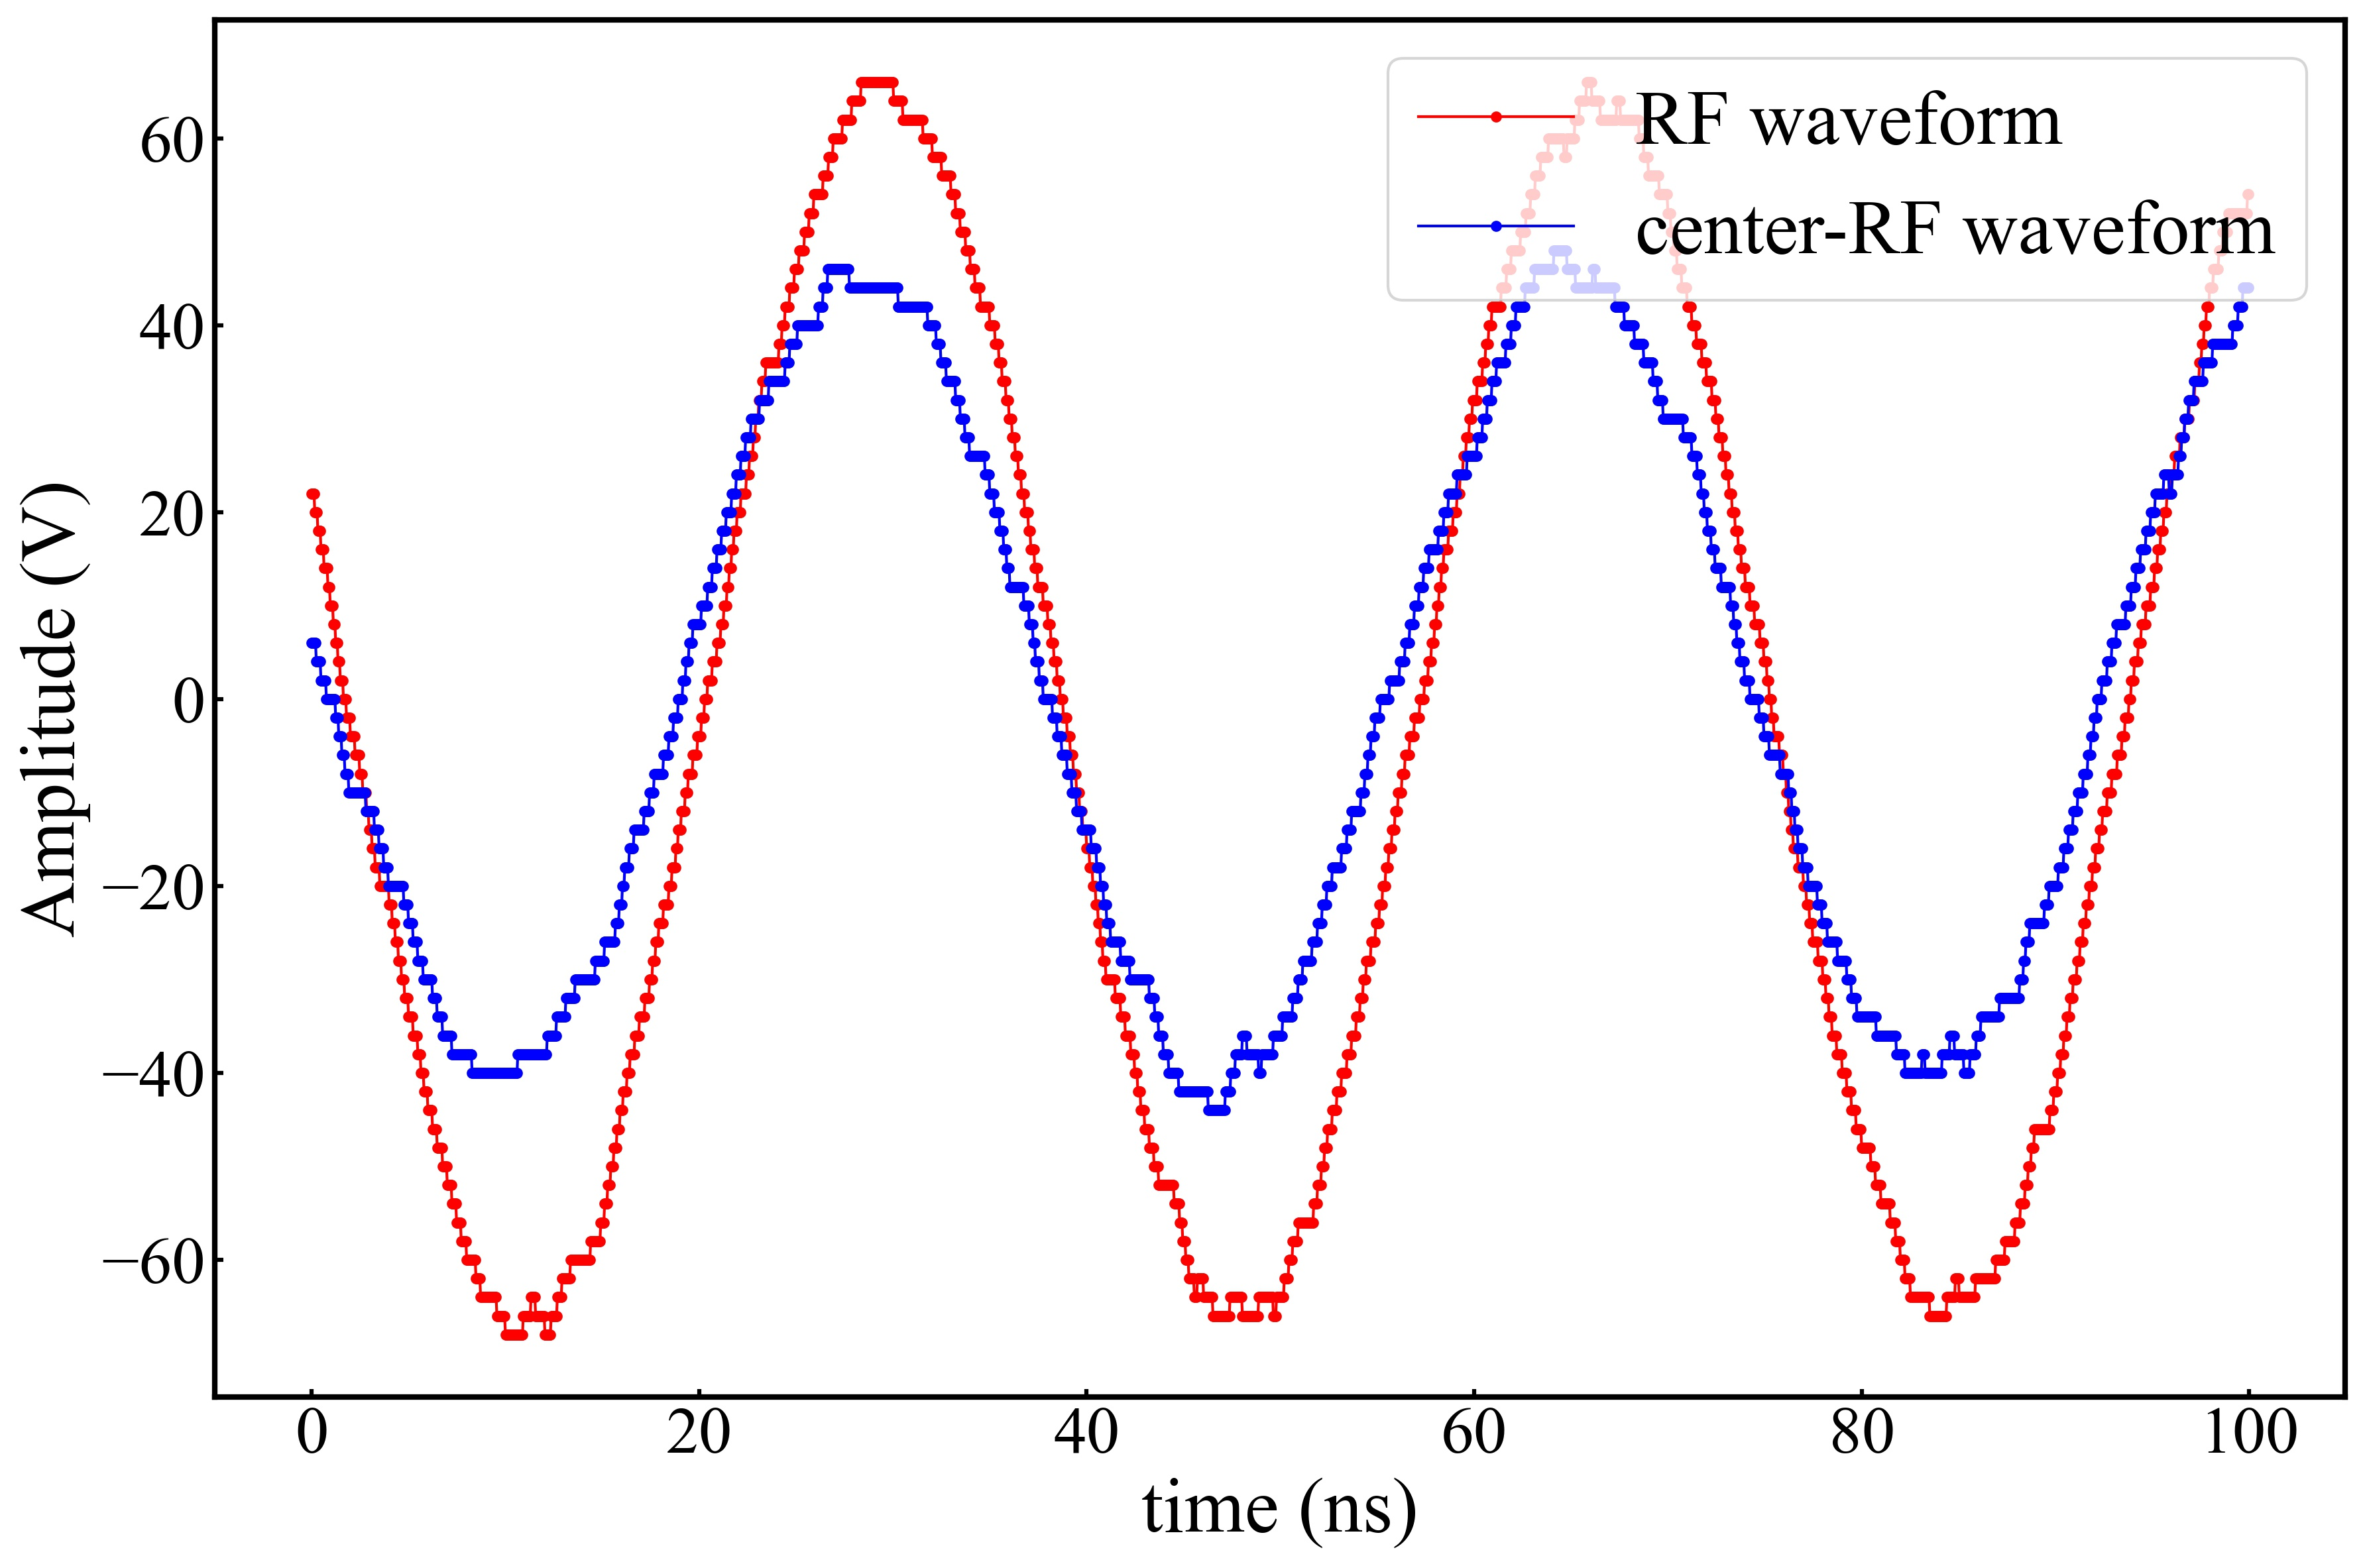
\includegraphics[width = 0.9\columnwidth]{./methods/figure/3_2D_wave.jpg}
			\caption{手順3におけるrf電圧とcenter-rf電圧の関係}
			\label{fig:3_2D_wave}
		\end{center}
	\end{minipage}
\end{figure}

このとき,$R=0.72$となっている.また,\Tb{3_2D}にマイクロメータの目盛を示す.

\begin{table}[h]
\begin{center}
	\caption{手順2におけるレンズの位置を調節するマイクロメータの目盛}
	\label{tab:3_2D}
	\begin{tabular}{c|cc} \hline \hline
		&鉛直方向&水平方向 \\ \hline
		垂直照射&43 & 1 \\ 
		斜め照射&18 & 1 \\ \hline
	\end{tabular}
\end{center}
\end{table}

この時点では,二列配列のポテンシャル形成はまだ行われていない.

\item さらにcenter-rf電圧の振幅を175mVppに設定する.\Fig{4_2D}にイオン捕獲画像を示し,\Fig{4_2D_wave}にrf電圧とcenter-rf電圧の関係を示す.

\begin{figure}[h]
	\begin{minipage}{0.48\linewidth}
	\begin{center}
		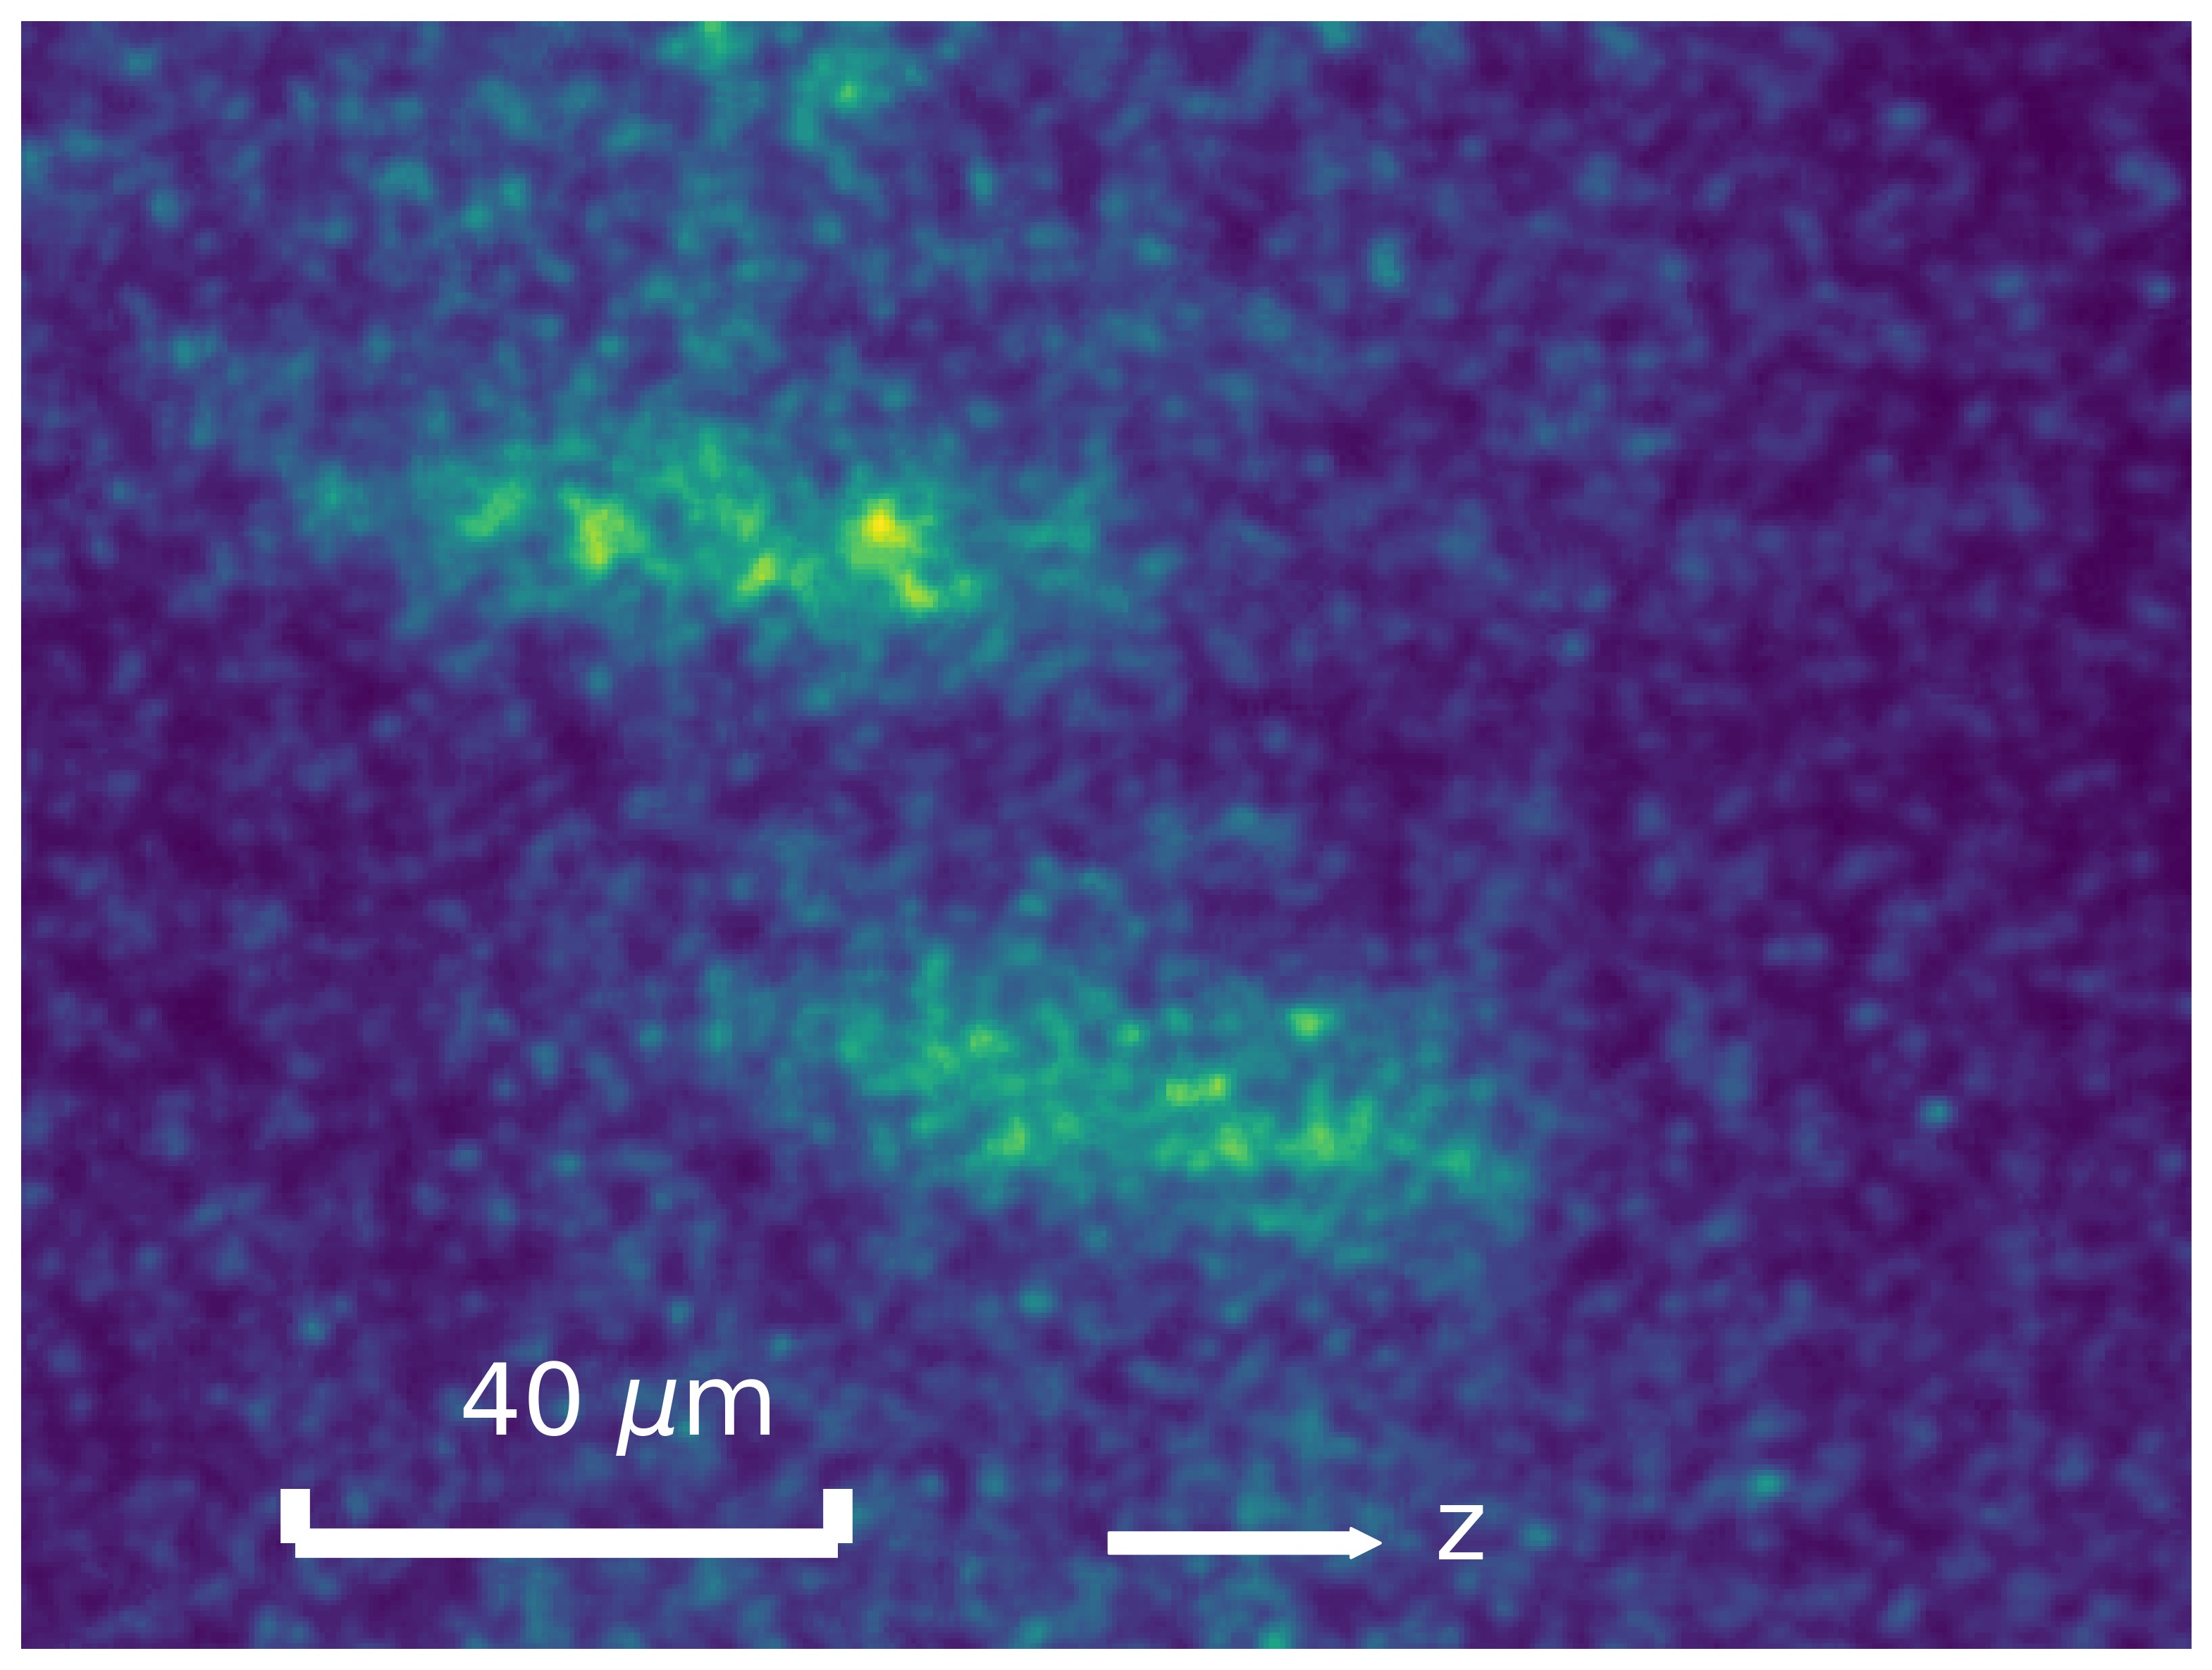
\includegraphics[width = 0.6\columnwidth]{./methods/figure/4_2D.jpg}
		\caption{手順4でのイオン捕獲画像}
		\label{fig:4_2D}
	\end{center}
	\end{minipage}
	\begin{minipage}{0.48\linewidth}
		\begin{center}
			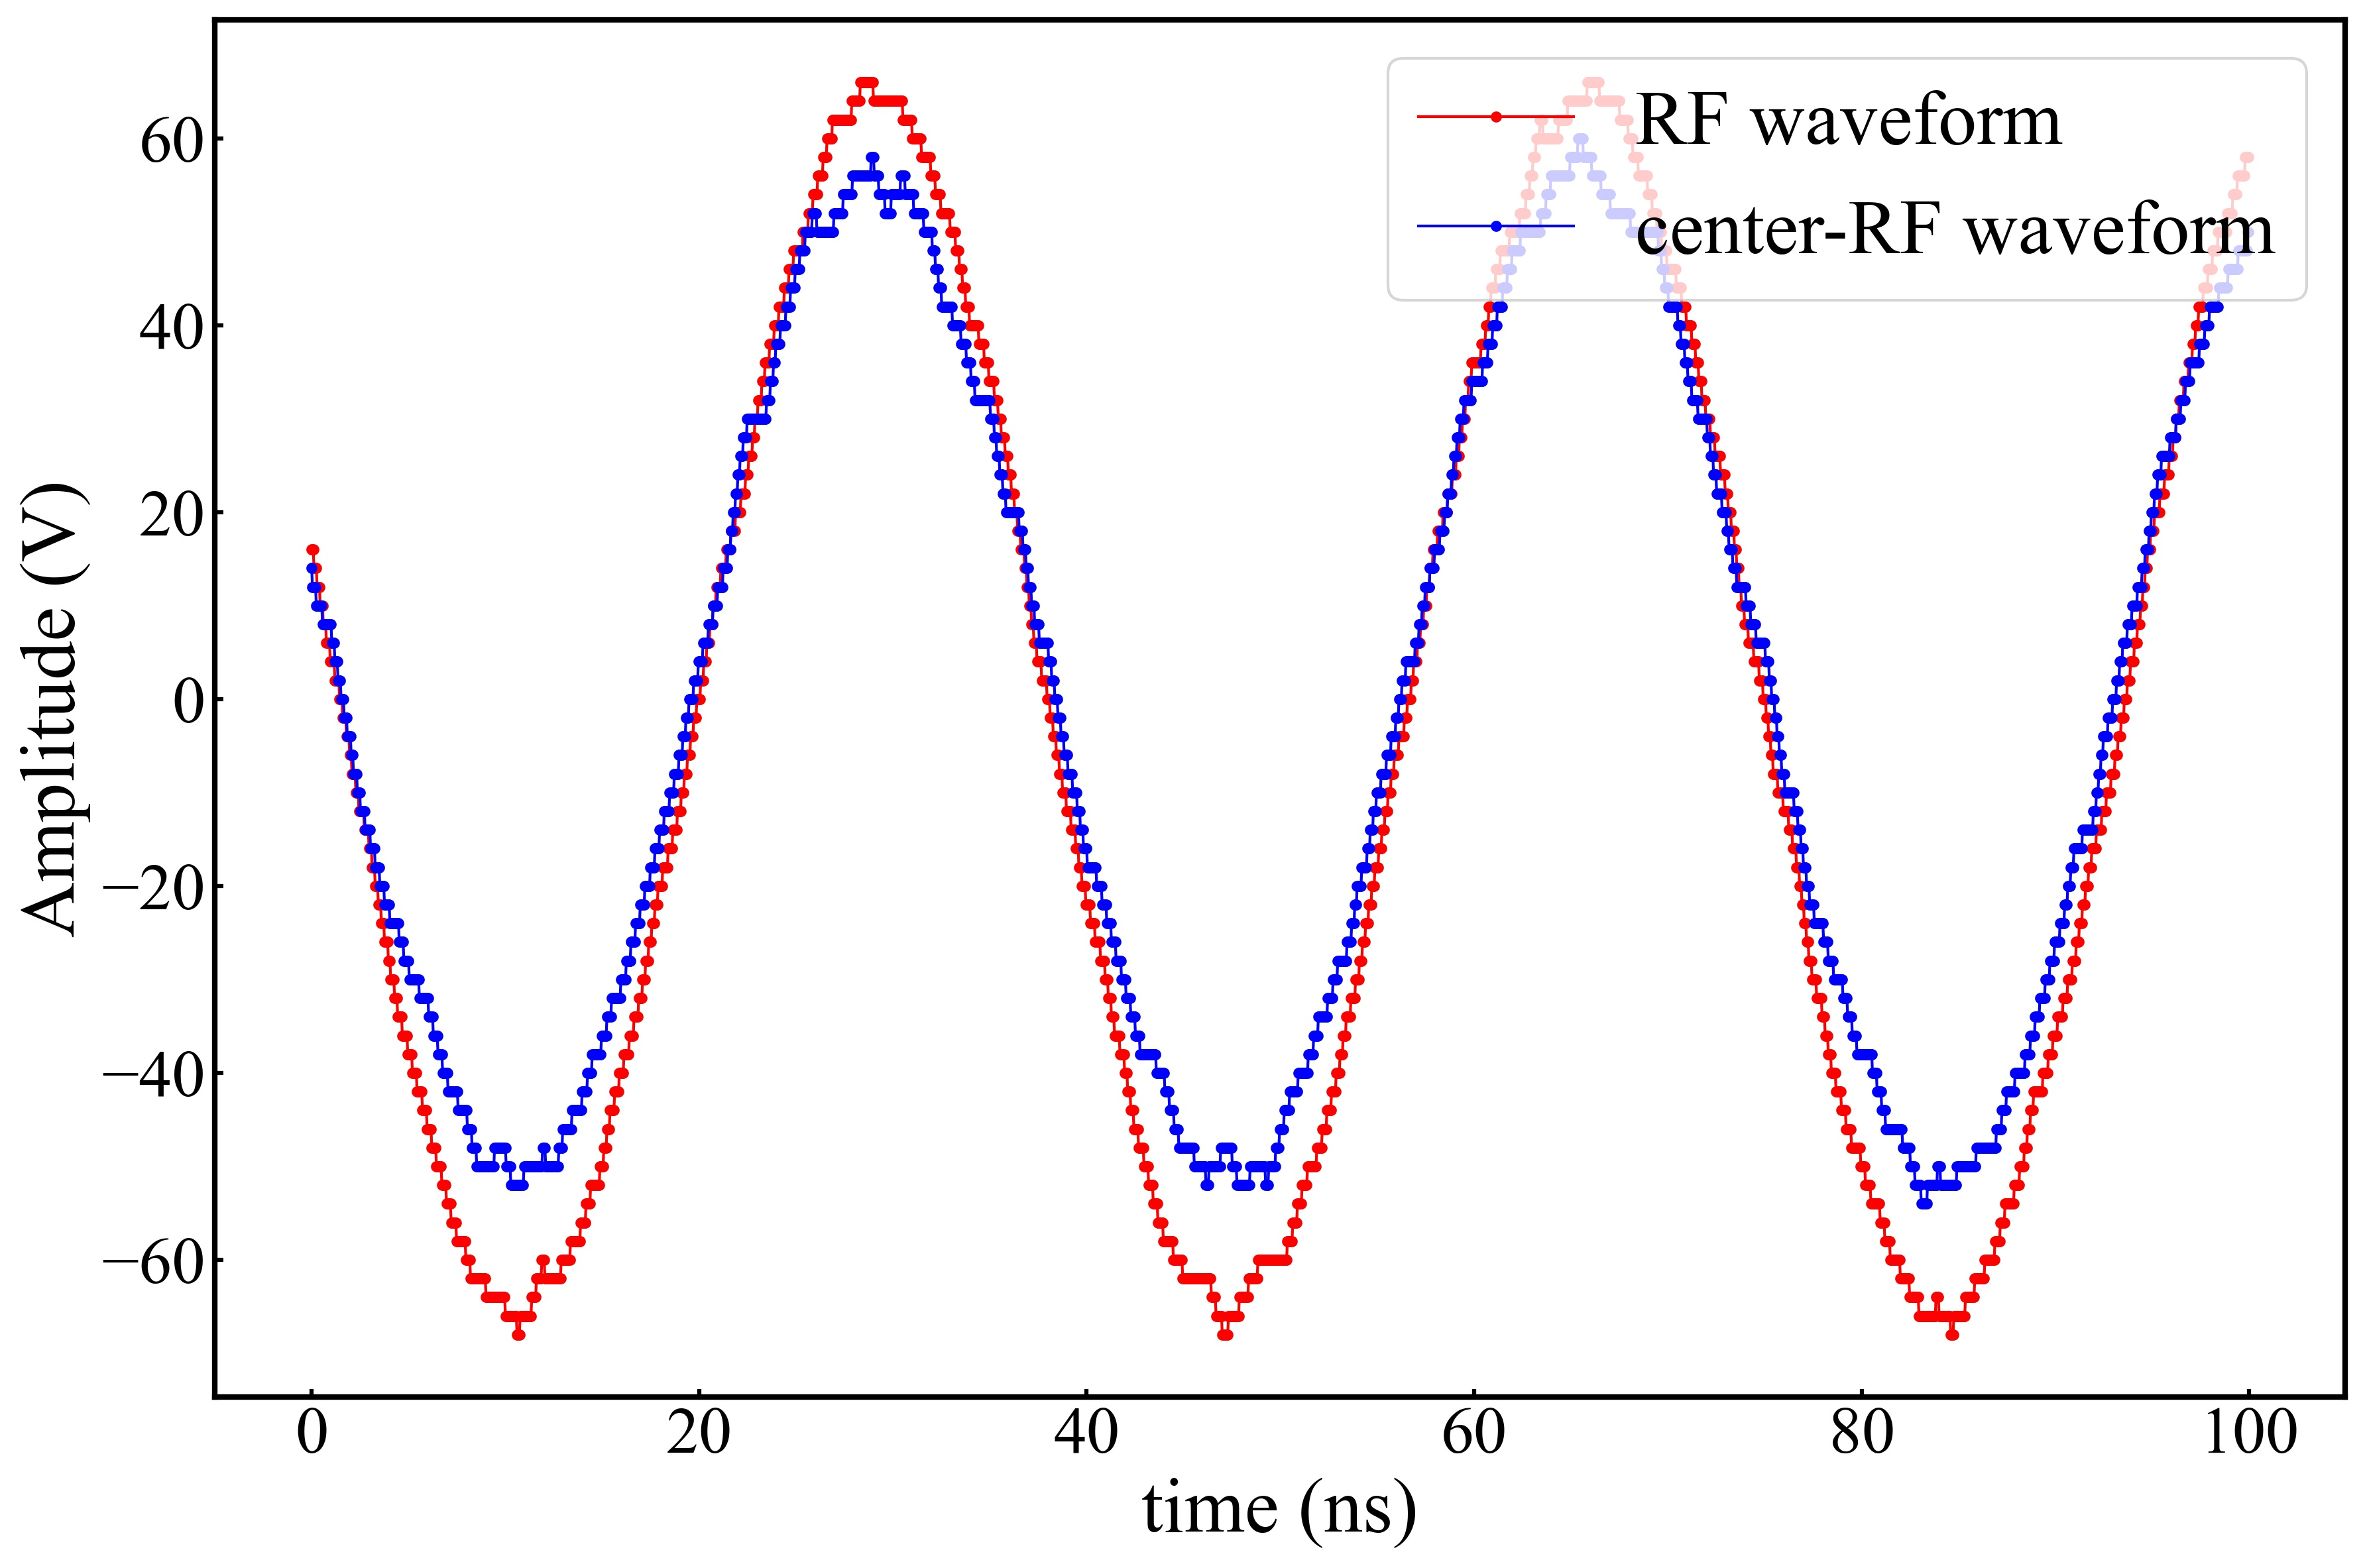
\includegraphics[width = 0.9\columnwidth]{./methods/figure/4_2D_wave.jpg}
			\caption{手順4におけるrf電圧とcenter-rf電圧の関係}
			\label{fig:4_2D_wave}
		\end{center}
	\end{minipage}
\end{figure}

このとき,$R=0.86$となっている.マイクロメータの目盛は\Tb{3_2D}から変更は行っていない.\Fig{4_2D}より,クラウド状でイオンが二列に捕獲されることが確認できる.また,center電極に印加する電圧を$V_{\rm center} = 0.335$V,side1電極に印加するdc電圧を$V_{\rm side1} = 0.383$Vに変更している.

\item 最後にcenter-rf電圧の振幅を180mVppに設定する.\Fig{5_2D}にイオン捕獲画像を示し,\Fig{5_2D_wave}にrf電圧とcenter-rf電圧の関係を示している.

\begin{figure}[h]
	\begin{minipage}{0.48\linewidth}
	\begin{center}
		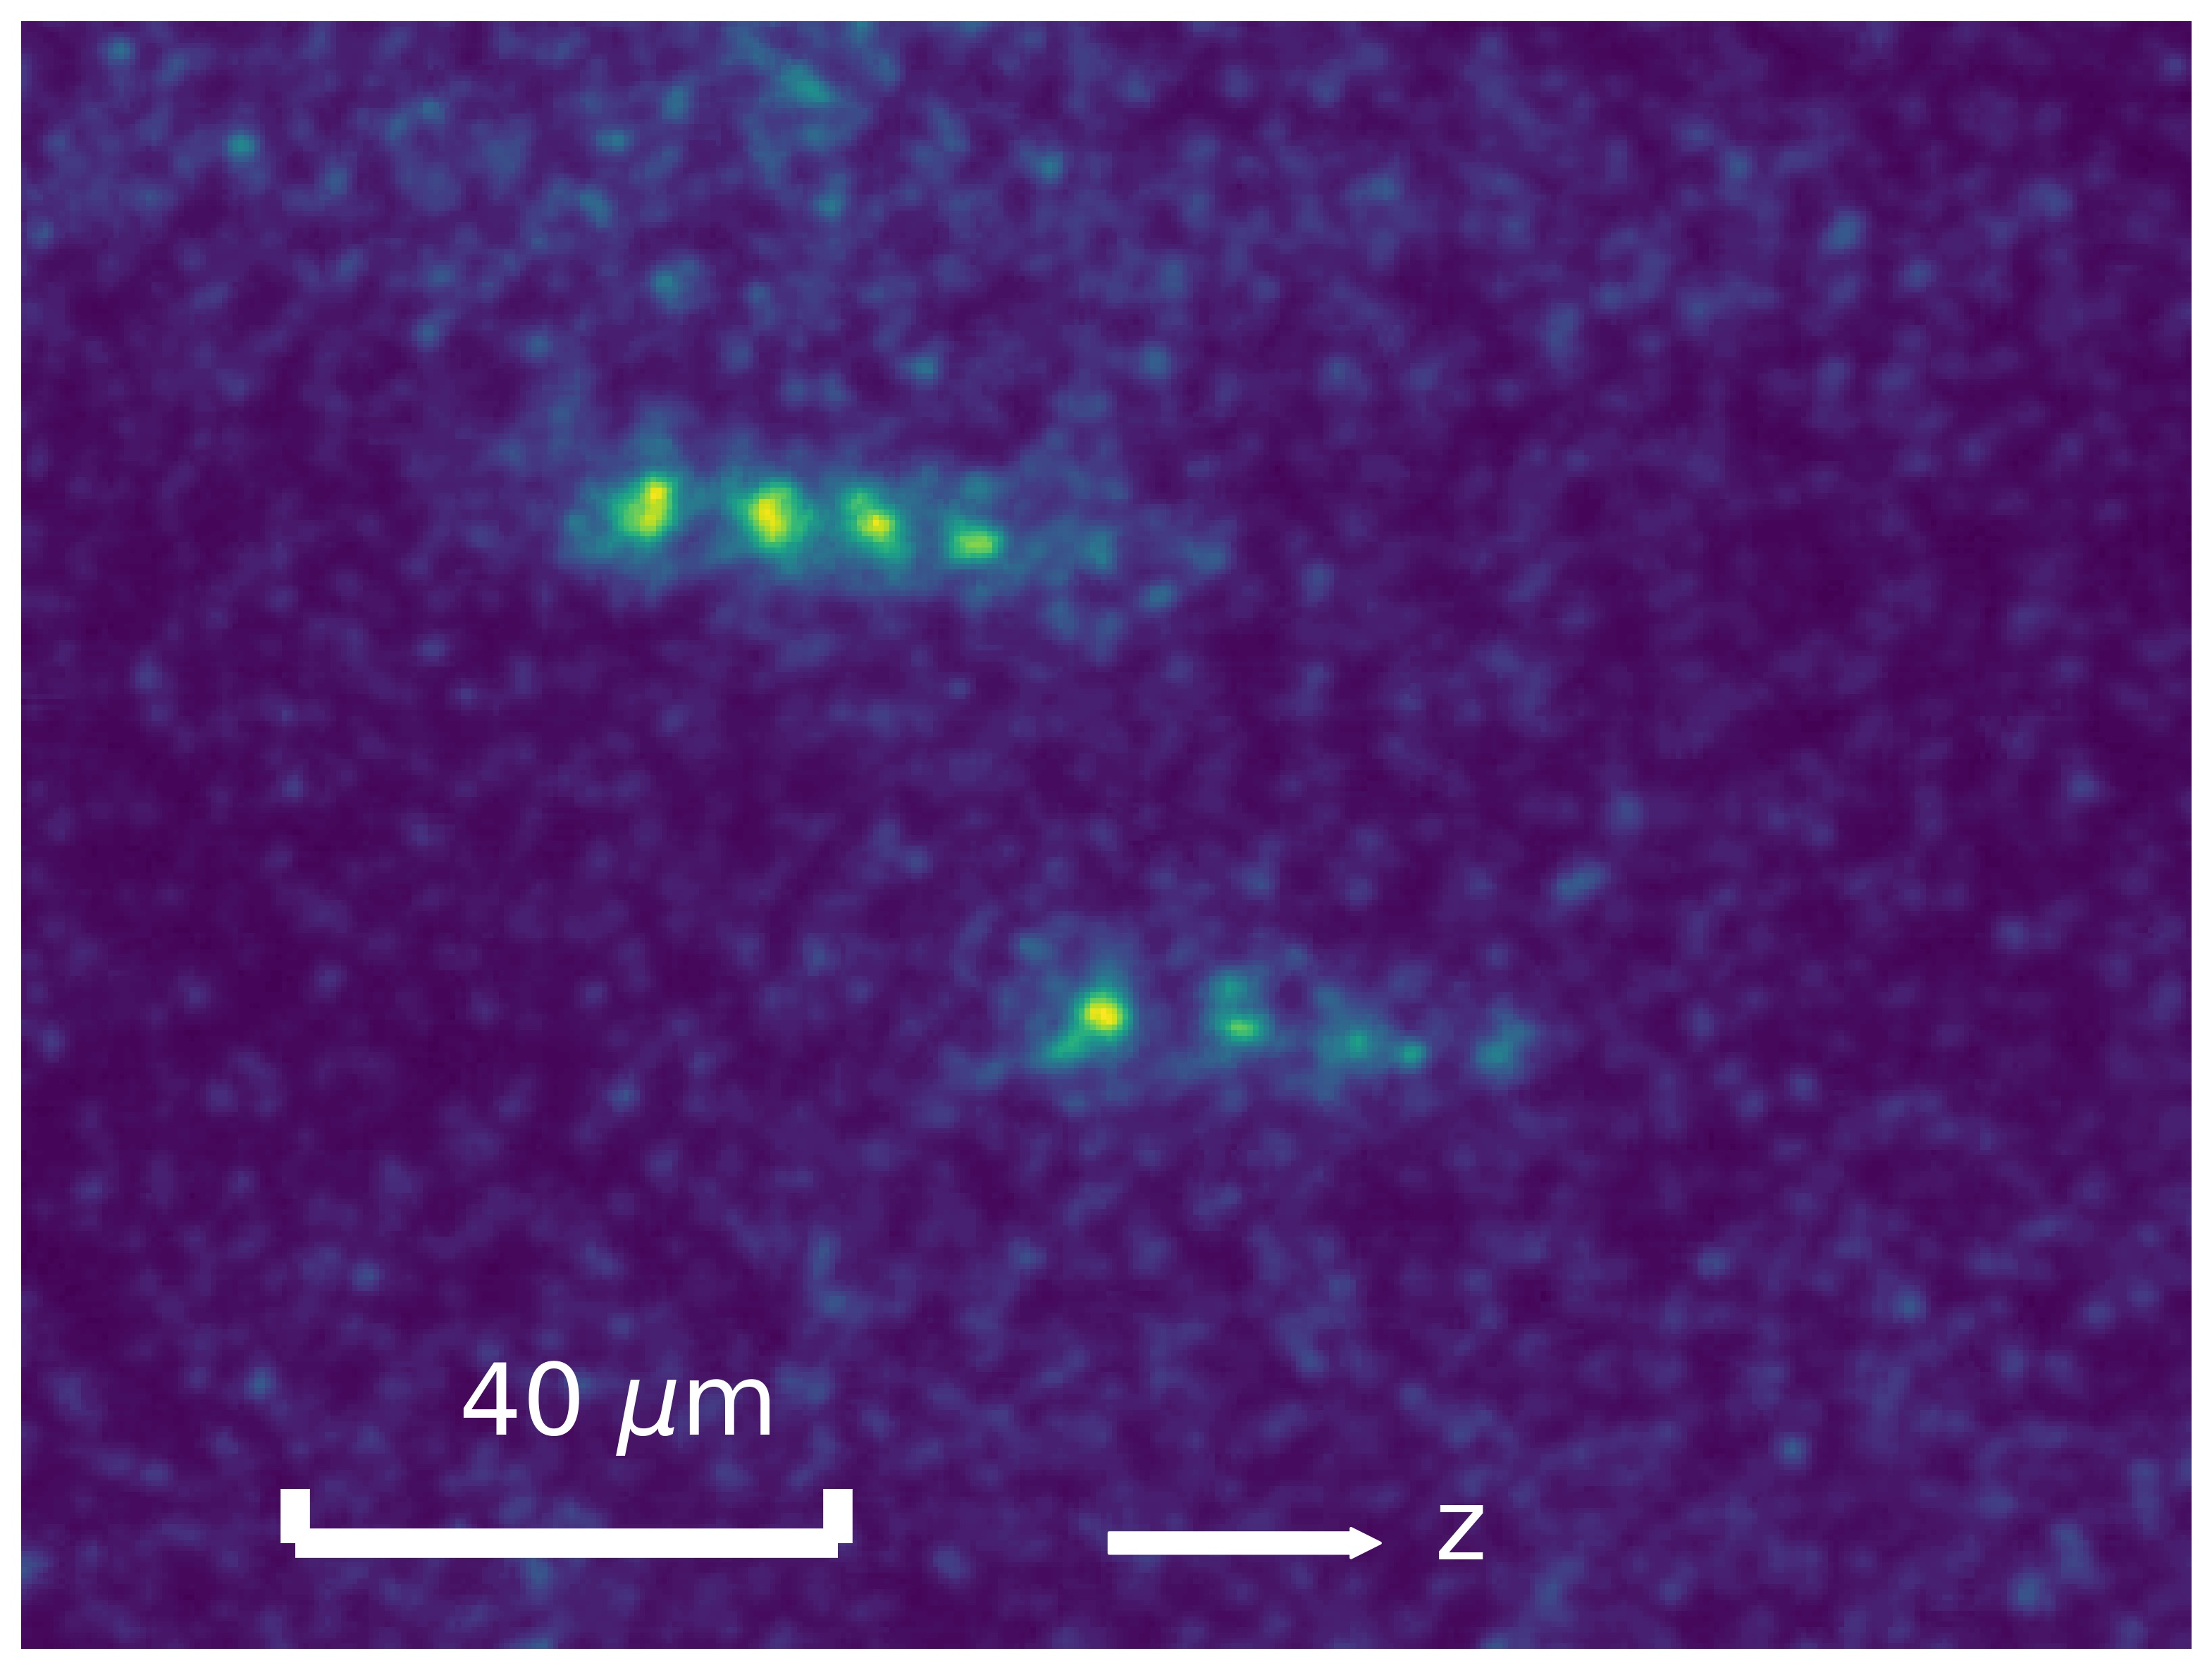
\includegraphics[width = 0.6\columnwidth]{./methods/figure/5_2D.jpg}
		\caption{手順5でのイオン捕獲画像}
		\label{fig:5_2D}
	\end{center}
	\end{minipage}
	\begin{minipage}{0.48\linewidth}
		\begin{center}
			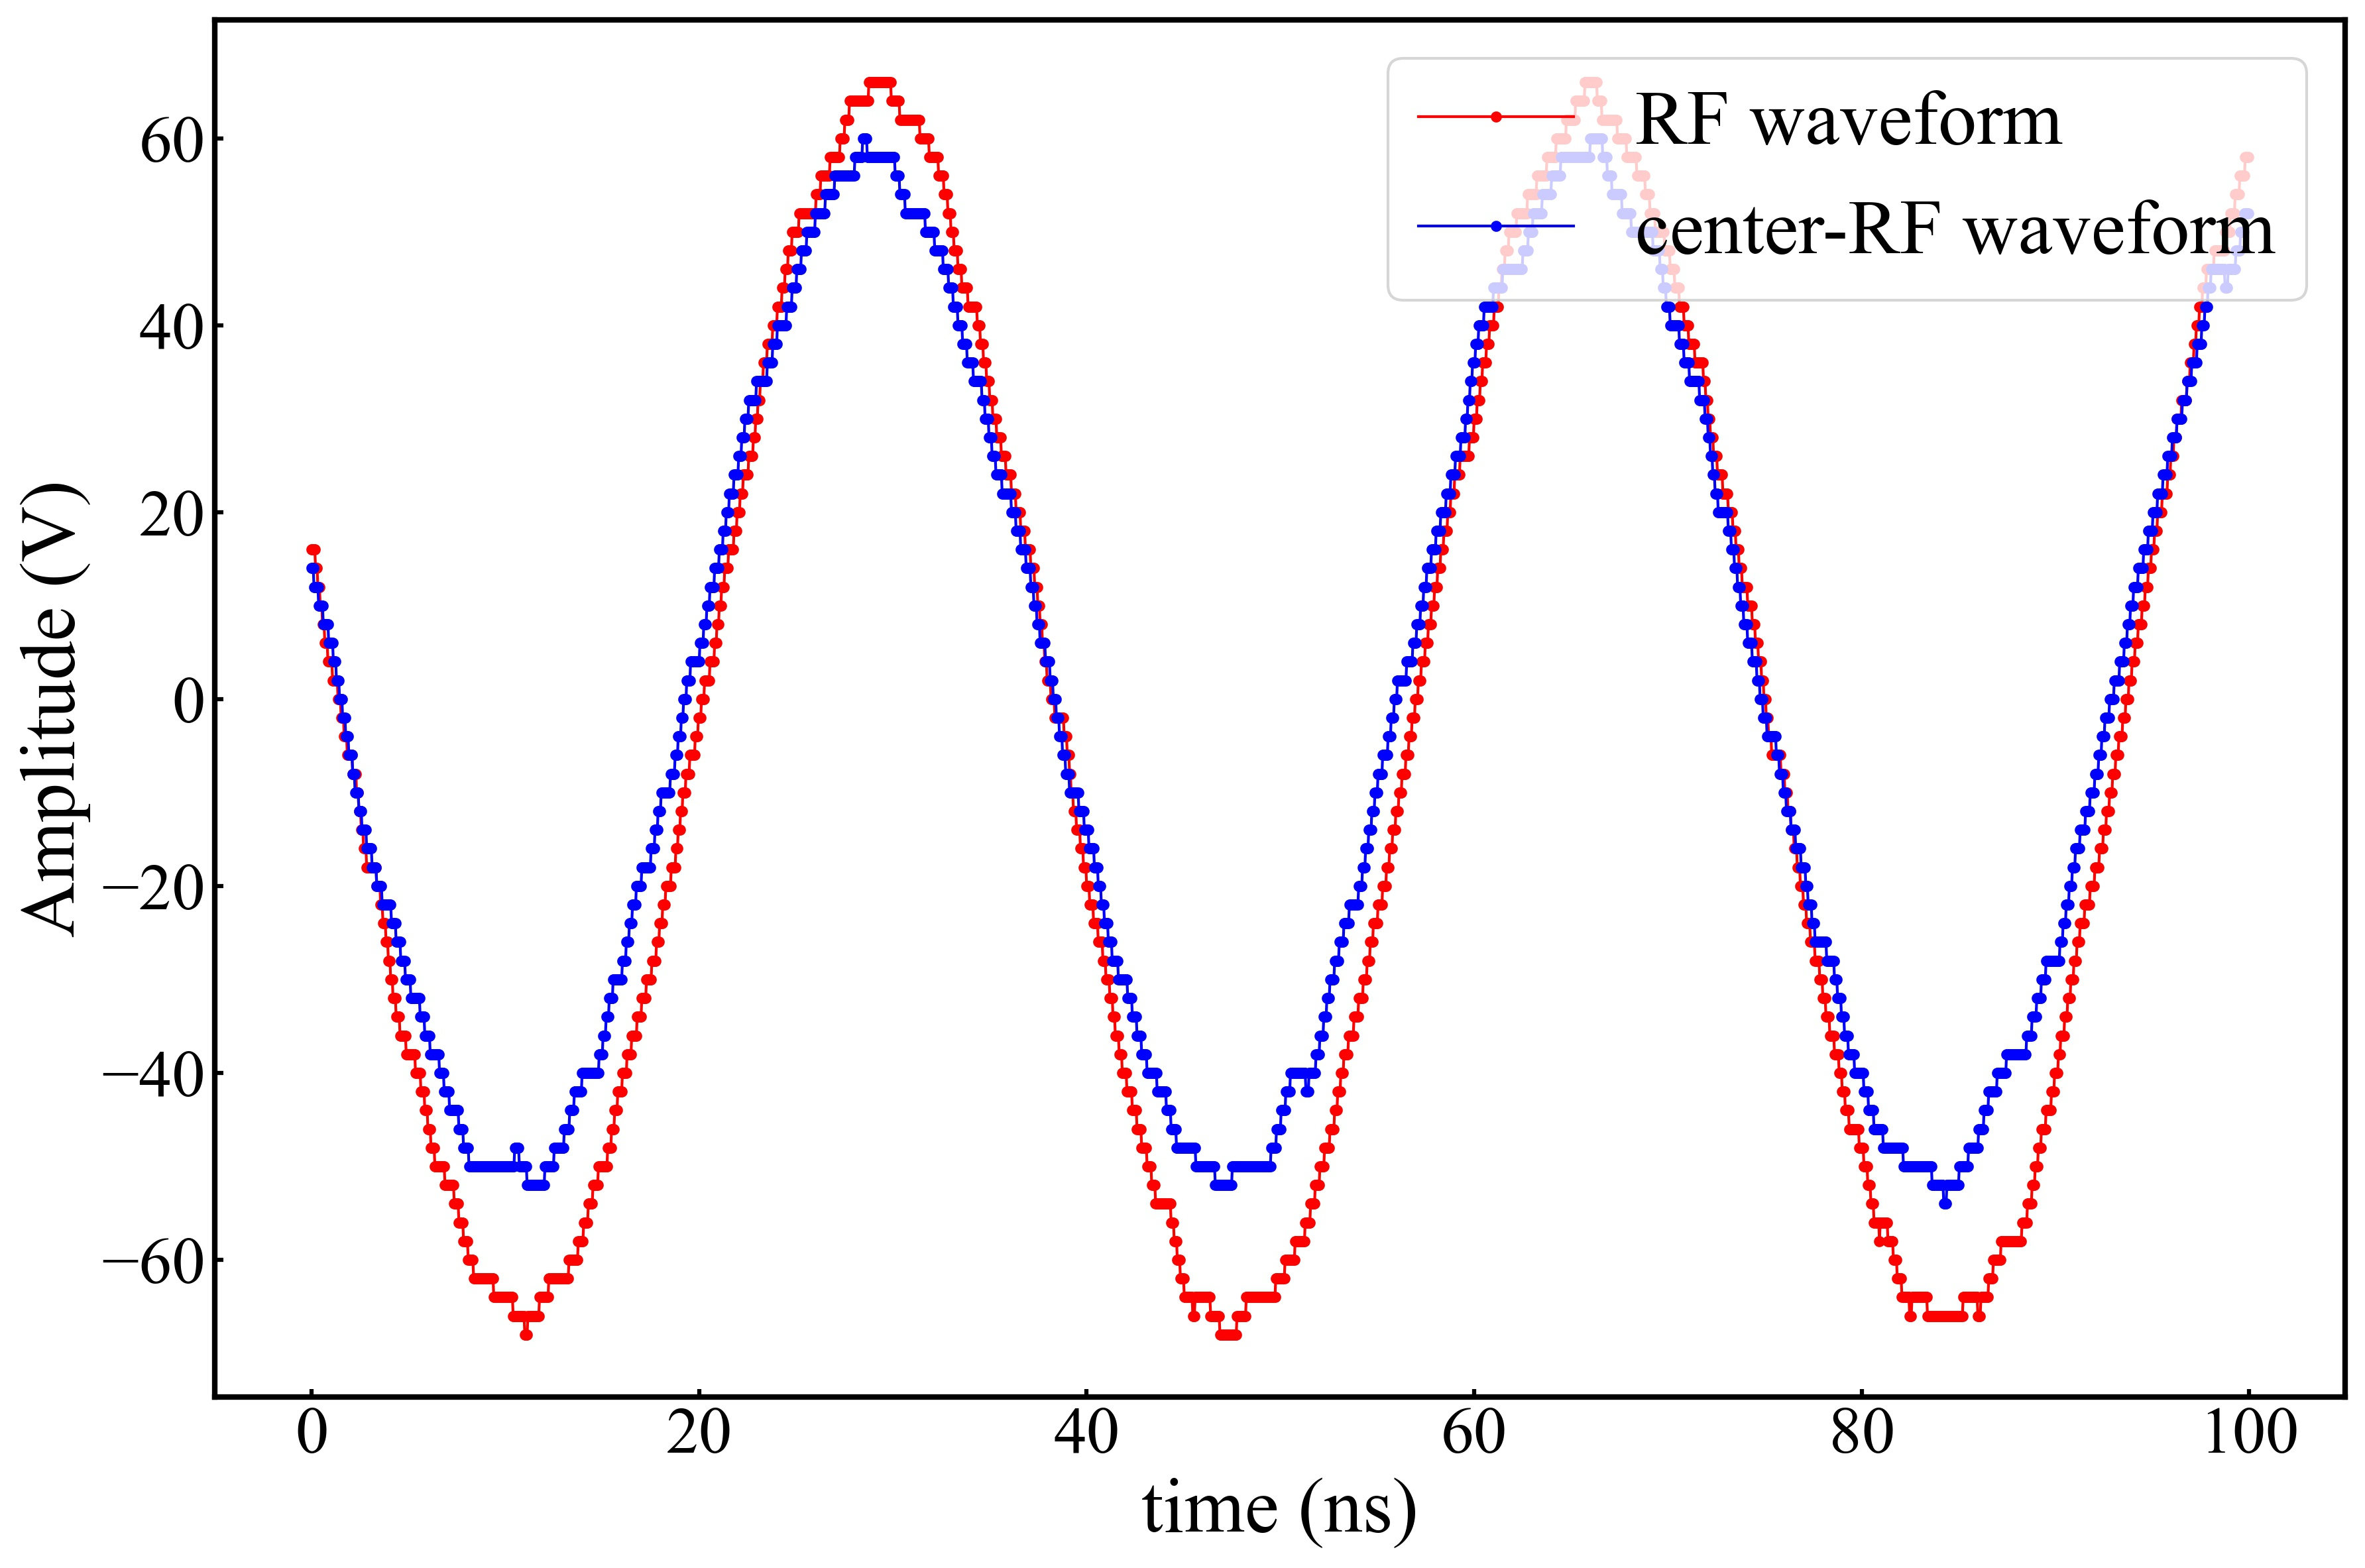
\includegraphics[width = 0.9\columnwidth]{./methods/figure/5_2D_wave.jpg}
			\caption{手順5におけるrf電圧とcenter-rf電圧の関係}
			\label{fig:5_2D_wave}
		\end{center}
	\end{minipage}
\end{figure}

このとき,$R=0.91$となっている.このとき,$V_{\rm center} = 0.225$Vにcenter電極に印加する電圧を変化させることでイオンの結晶化が観測される.

\end{enumerate}

\clearpage

\section{永年周波数の測定方法} \label{MaesSecFreq_Mathod}
永年周波数の測定システムの開発を行った.dc電極にac信号を重畳させることでイオンに強制振動を引き起こすことが可能である.共鳴時,イオンの蛍光量が減少し,また,その振幅が広がることが画像から確認することができた.本実験では,\Fig{MeasSec_System}に示すF.G.2からの信号をmiddle1電極に印加し周波数の掃引を行うことで,イオンの振幅の周波数特性を取得し,ローレンツ分布関数によるフィッティングを行うことで永年周波数の測定を行った.また,イオンの振幅を計測するにあたり,S/N比を向上させるため積算回数を15回としている.

\begin{figure}[h]
	\centering
	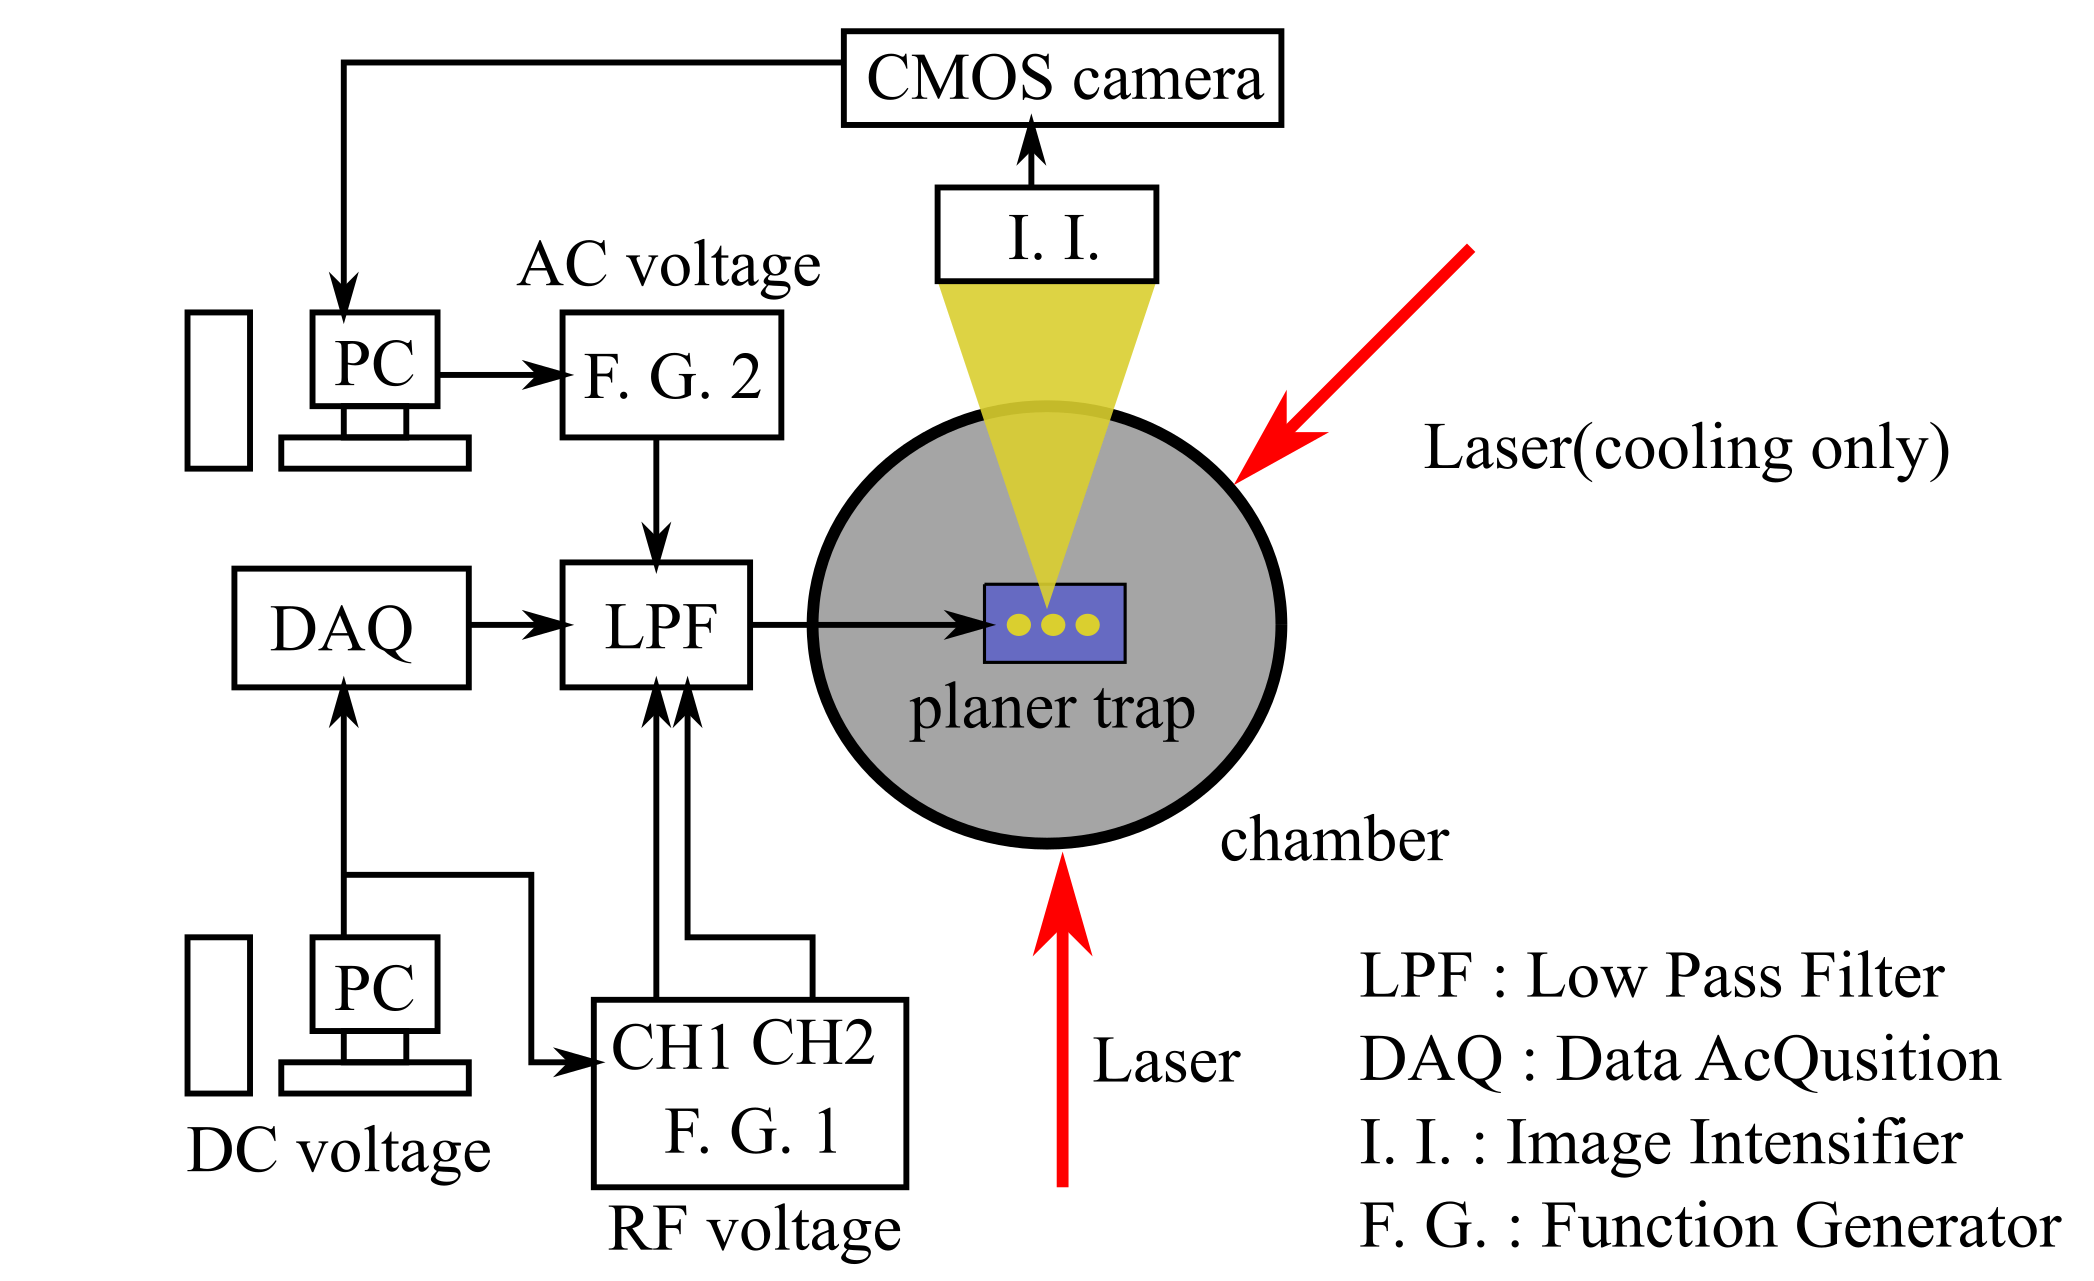
\includegraphics[width = 0.6\linewidth]{./methods/figure/SecularFreqMeasSetup.png}
	\caption{永年周波数測定のための実験系}
	\label{fig:MeasSec_System}
\end{figure}

\Fig{example_off_resonance}と\Fig{example_resonance}に非共鳴時と共鳴時(z方向)のイオンの振幅の様子を示す.

\begin{figure}[h]
		\begin{minipage}{0.48\linewidth}
			\centering
			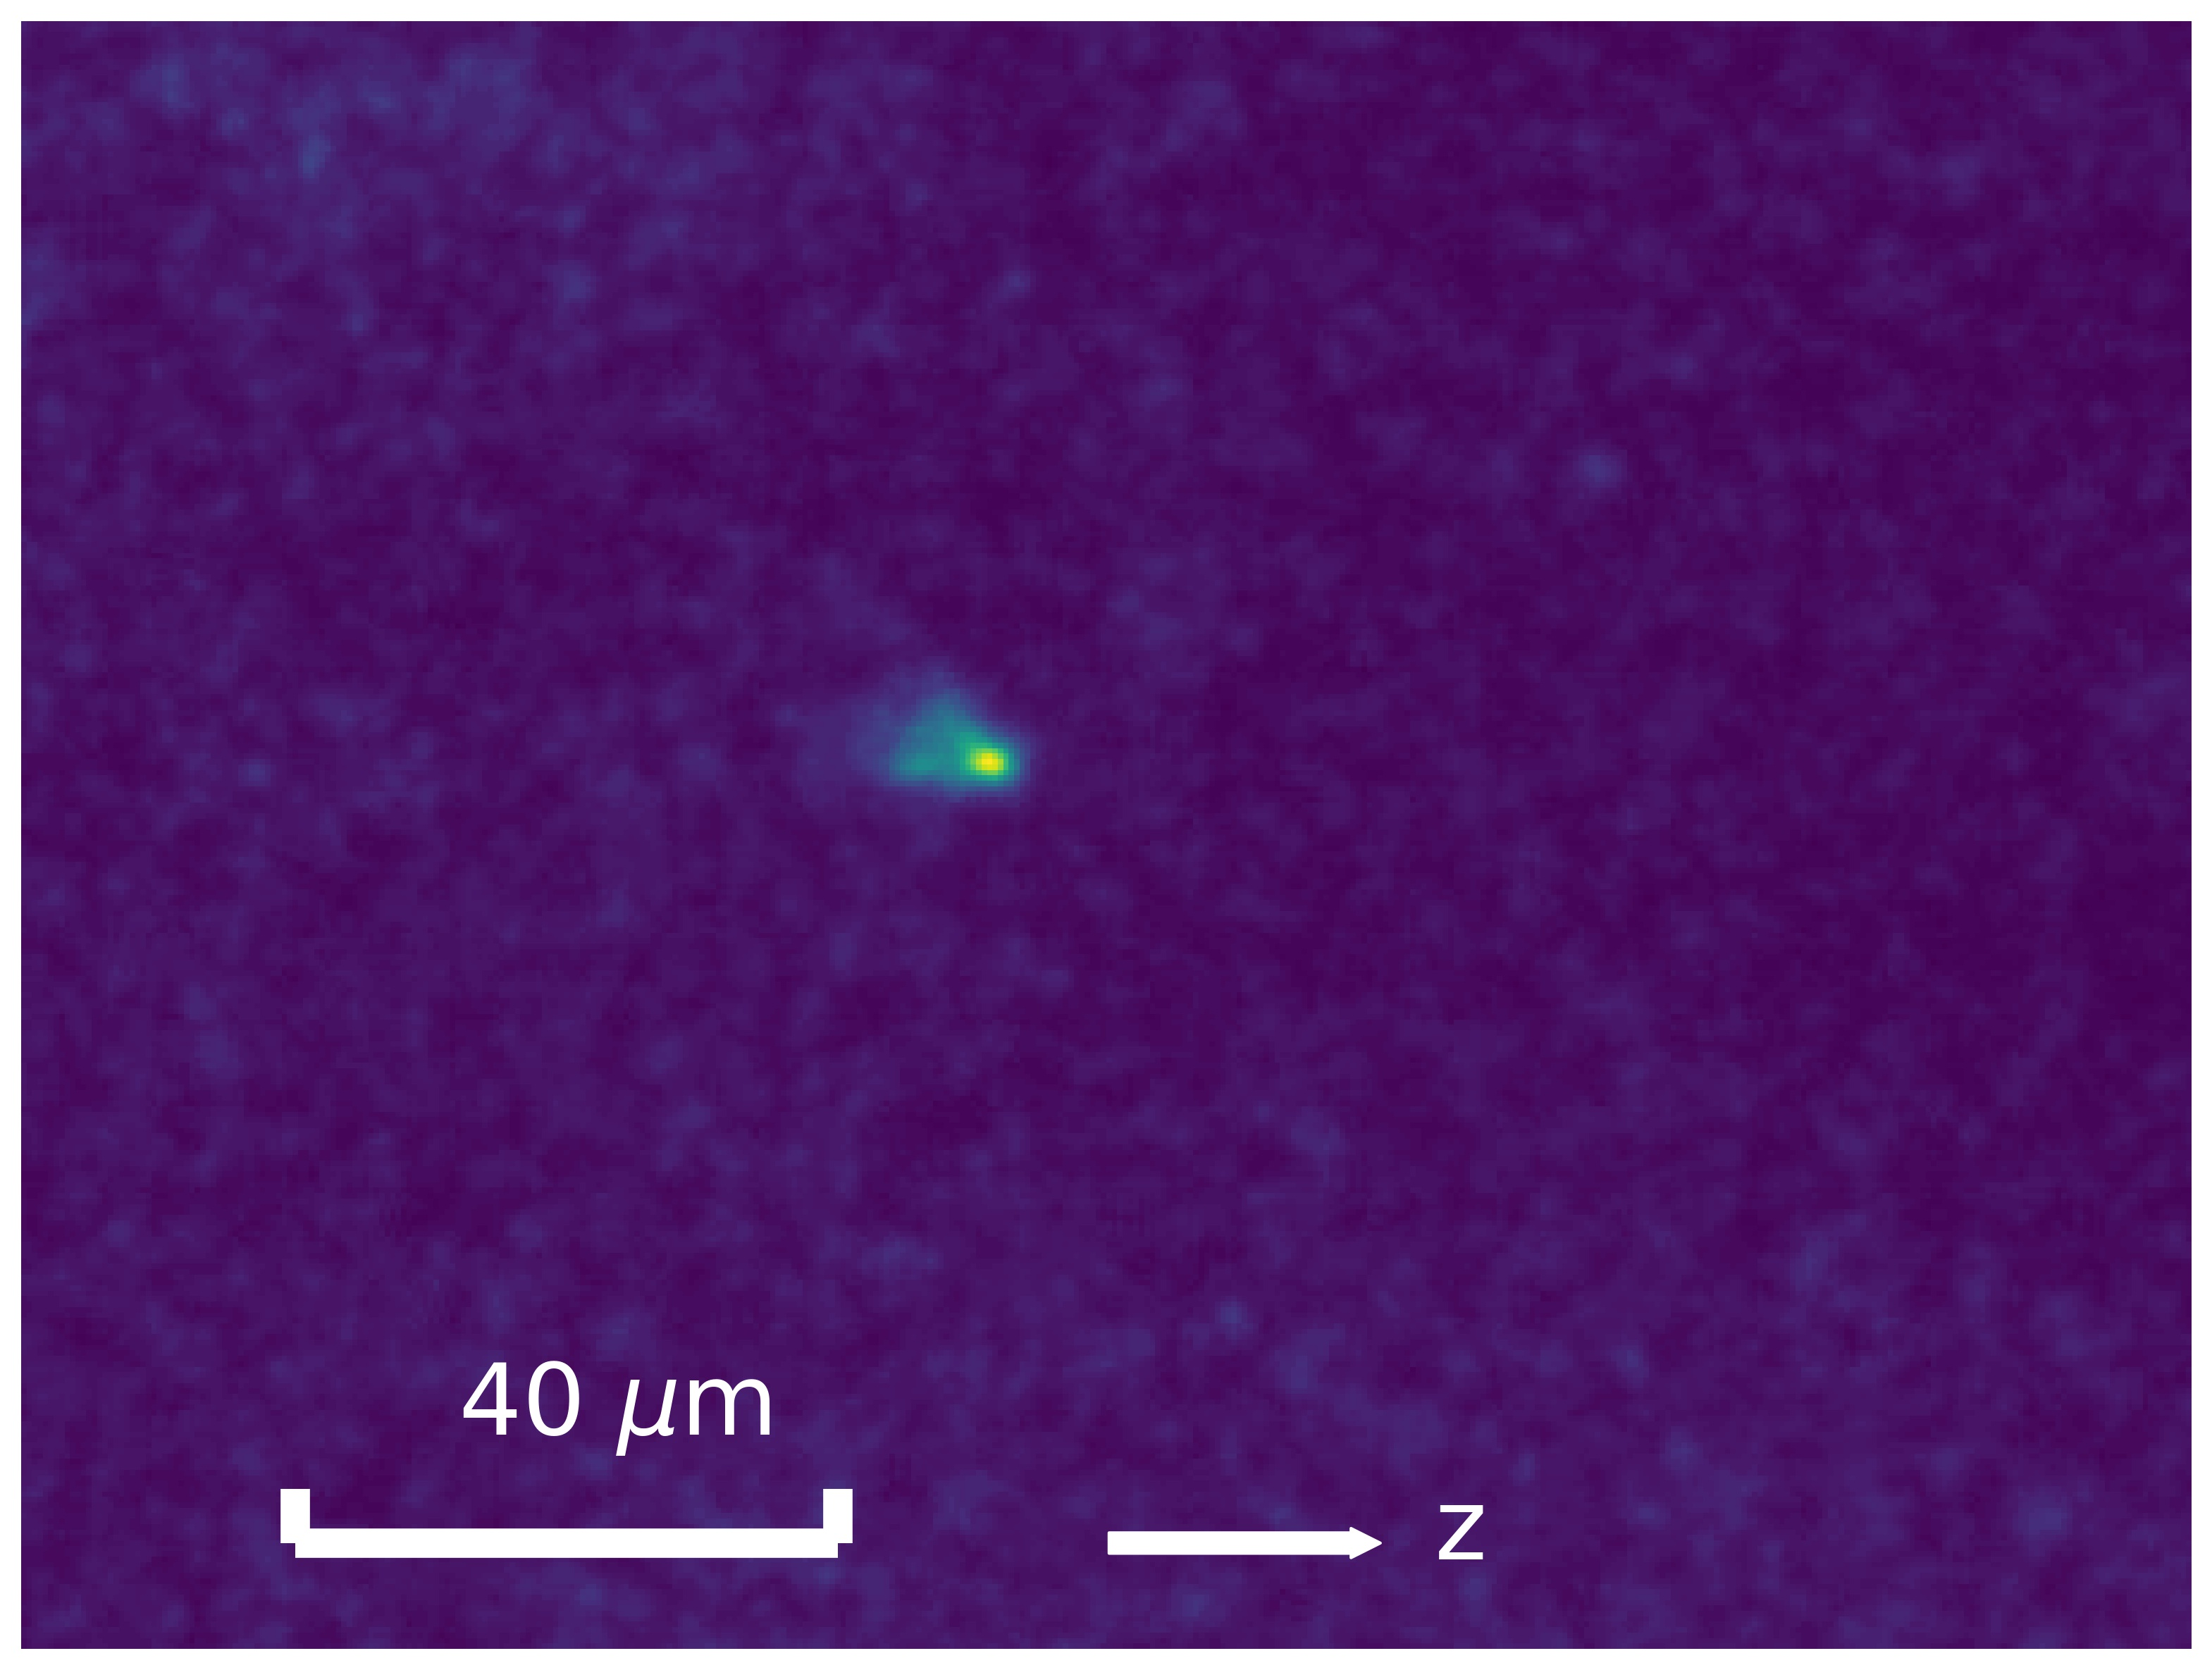
\includegraphics[width = 0.6\columnwidth]{./methods/figure/off_resonance.jpg}
			\caption{非共鳴時のイオンの捕獲画像}
			\label{fig:example_off_resonance}
		\end{minipage}
		\begin{minipage}{0.48\linewidth}
			\centering
			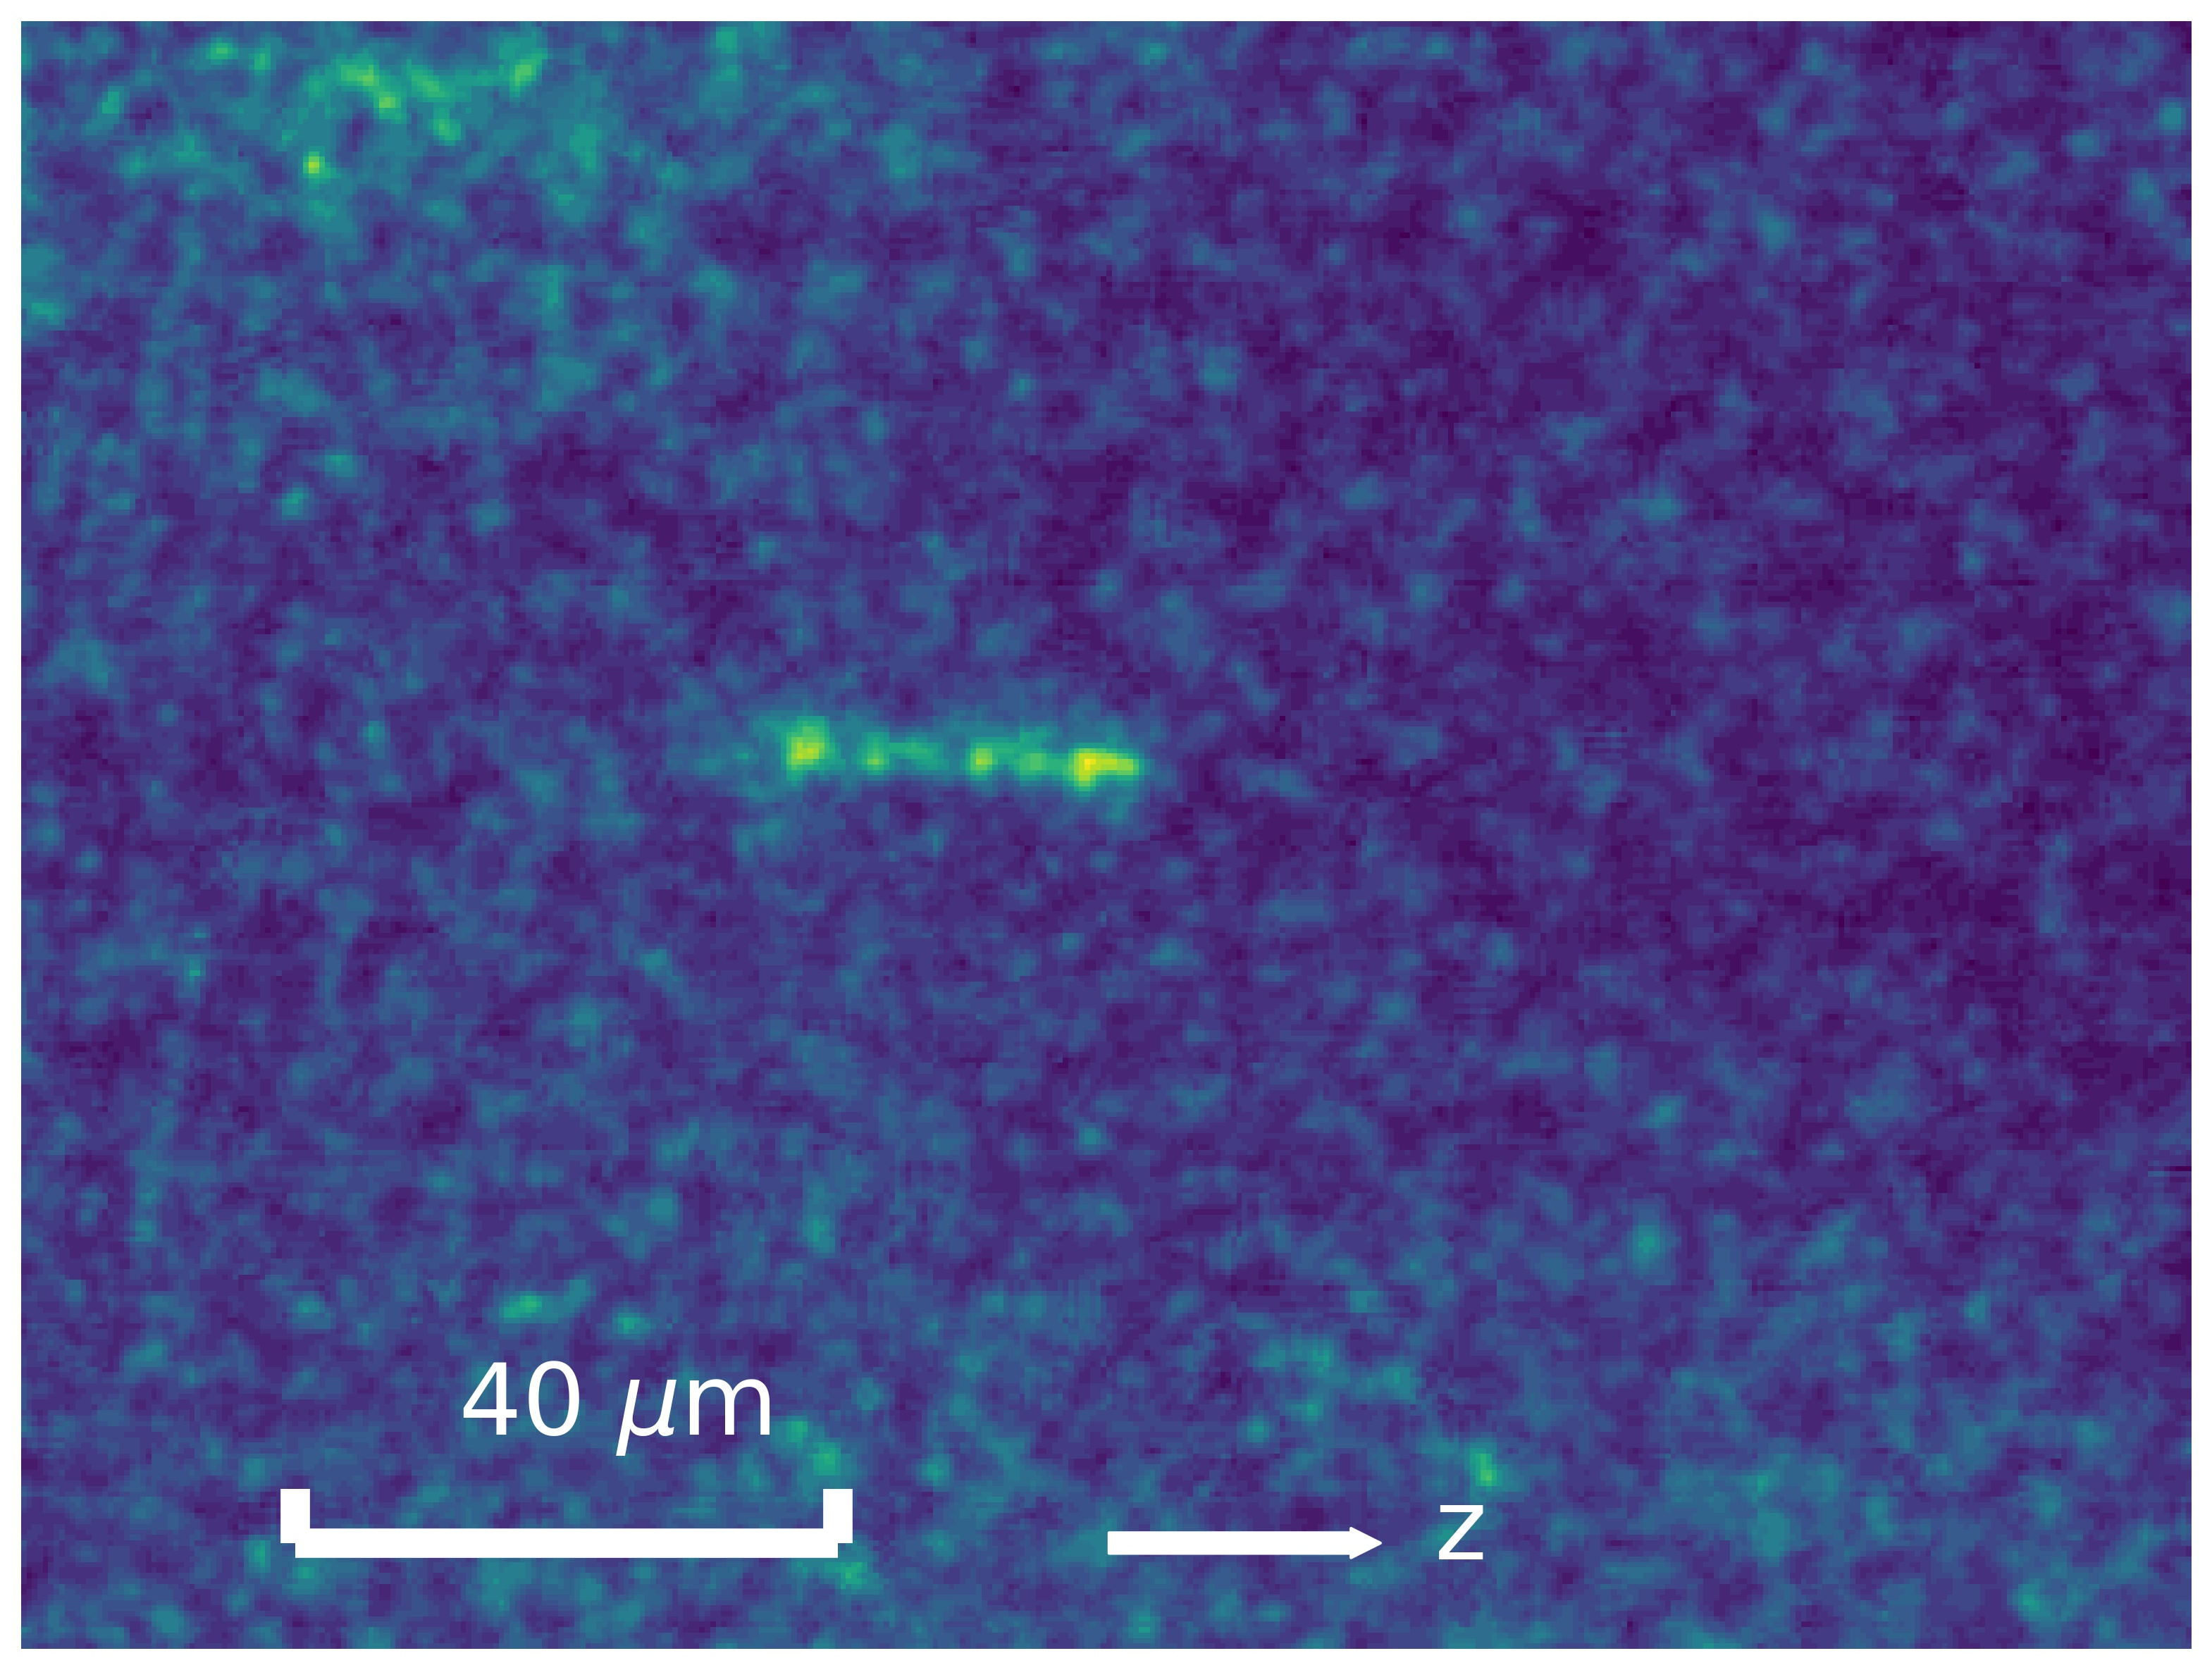
\includegraphics[width = 0.6\columnwidth]{./methods/figure/resonance.jpg}
			\caption{共鳴時のイオンの捕獲画像}
			\label{fig:example_resonance}
		\end{minipage}
\end{figure}

\Fig{fitting_result}に\Tb{dc_string}に示すdc電圧セットにおいて取得されたイオンの振幅の周波数特性と,そのフィッティング結果を示す.

\begin{figure}[h]
	\centering
		\includegraphics[width = 0.4\linewidth]{./methods/figure/fitting_result.jpg}
		\caption{\Tb{dc_string}のdc電圧セットに対するイオンの振幅の周波数特性とフィッティング結果}
		\label{fig:fitting_result}
\end{figure}

フィッティング結果より,z方向の永年周波数は

\begin{align}
\left( \frac{\omega_z}{2\pi}\right) = 216.4 \pm 0.32 \  {\rm kHz} \notag
\end{align}

であることが分かる.なお,このときのac信号の振幅は200 mVppで周波数掃引は215 kHzから218 kHzまで50 Hz刻みで行った.

\section{イオン捕獲位置における電場の算出方法}

Python3.6の環境において,NumPyとOpenCVのモジュールを利用して,イオン捕獲画像のヒストグラムの正規化および二値化を行い,イオンの位置特定を行った.カメラから得られるイオン捕獲画像を\Fig{raw_image}に示す.そして,イオンの位置特定の際の処理速度および精度の向上のため,\Fig{rect_image}に示す範囲でヒストグラムの処理を行う.

\begin{figure}[h]
	\begin{minipage}{0.48\linewidth}
		\begin{center}
			\includegraphics[width=0.6\columnwidth]{./methods/figure/raw_image.png}
			\caption{CCDカメラから得られるイオンの捕獲画像}
			\label{fig:raw_image}
		\end{center}
	\end{minipage}
	\begin{minipage}{0.48\linewidth}
		\begin{center}
			\includegraphics[width=0.6\columnwidth]{./methods/figure/rect_image.png}
			\caption{\Fig{raw_image}において画像処理を実行する範囲}
			\label{fig:rect_image}
		\end{center}
	\end{minipage}
\end{figure}

そして,得られたイオンの位置から平衡の式\Eq{equi_string}を用いてイオン捕獲位置における電場$\bm{E}(z_{i})$の算出を行った.

\begin{figure}[h]
	\begin{center}
		\includegraphics[scale=0.5]{./methods/figure/out_image.png}
		\caption{イオンの位置特定を行い,平衡の式\Eq{equi_string}を用いて算出した電場の大きさと向き(赤丸はイオンの位置を示し,青色の矢印の長さと向きは電場の大きさと向きを示している)}
		\label{fig:out_image}
	\end{center}
\end{figure}

\Fig{out_image}から算出された電場は,左から数えて1,2と番号を振ったとき,

\begin{align*}
	E_{1,z} &= 5.603 \ {\rm V/m} \\
	E_{2,z} &= -5.603 \ {\rm V/m} 
\end{align*}

となる.
	% -- 実験結果 -- %
	\chapter{実験結果}
\section{一列配列イオン}
\subsection{イオン捕獲位置のdc電圧依存性}
プレーナートラップのdc電極に印加するdc電圧を変化させたときのイオン捕獲位置の変位と,シミュレーション結果におけるイオン捕獲位置の変位を単一イオンを用いて比較し,シミュレーションの精度の確認を行った.\Tb{dc_string}に示したdc電圧セットにおいて,$V_{\rm End 1}, \ V_{\rm End3}$および$V_{\rm End 2}, \ V_{\rm End4}$を$0.54 \ {\rm V} \ \sim \ 2.84 \ {\rm V}$まで$0.1 {\rm V}$ずつ変化させたときのイオン捕獲位置の変位について実験を行った.\Fig{displacement_End13}に$V_{\rm End 1} \ = \ V_{\rm End3} = $0.54 V (a), 1.14 V (b), 1.44 V (c), 1.84 V (d), 2.34 V (e), 2.84 V (f)としたときのイオン捕獲画像を示す.

\begin{figure}[h]
	\begin{center}
		\includegraphics[width = 0.6 \linewidth]{./results/figure/displacement_End_Odd.png}
		\caption{$V_{\rm End1}, V_{\rm End3} = 0.54{\rm \ (a)}, \ 1.14{\rm \ (b)}, \ 1.44{\rm \ (c)}, \ 1.84{\rm \ (d)}, \ 2.34{\rm \ (e)}, \ 2.84{\rm \ (f)} \ {\rm V}$のときのイオン捕獲画像}
		\label{fig:displacement_End13}
	\end{center}
\end{figure}

\Fig{displacement_End13}より,End1とEnd3に印加するdc電圧を大きくしていくと$+z$方向へとイオン捕獲位置が変位し,dc電圧を小さくしていくと$-z$方向へ変位することが確認できた.
%
\clearpage
%
\Tb{dc_string}の条件におけるイオン捕獲位置を基準とし,$V_{\rm End1}, \ V_{\rm End3}$の変化に対するイオン捕獲位置の変位とシミュレーション上でのイオン捕獲位置の変位との比較を\Fig{sim_exp_displacement_End13}に示す.なお,シミュレーション上でのイオン捕獲位置は,プレーナートラップ電極モデルのx=0におけるSecularポテンシャルの最小値としている.
\begin{figure}[h]
	\begin{center}
		\includegraphics[width = 0.6\linewidth]{./results/figure/out_V13.jpg}
		\caption{\Tb{dc_string}の条件にて${\rm V}_{\rm End1}$と${\rm V}_{\rm End3}$の値を$0.54 \sim 2.84$Vまで0.1Vずつ変化させたときのイオン捕獲位置の変位の実験値とシミュレーション値との比較}
		\label{fig:sim_exp_displacement_End13}
	\end{center}
\end{figure}

$V_{\rm End2}, \ V_{\rm End4}$の電圧値を変化させて同様の実験を行った.実験値とシミュレーション値との比較を\Fig{sim_exp_displacement_End24}に示す.

\begin{figure}[h]
	\begin{center}
		\includegraphics[width = 0.6\linewidth]{./results/figure/out_V24.jpg}
		\caption{\Tb{dc_string}の条件にて${\rm V}_{\rm End2}$と${\rm V}_{\rm End4}$の値を$0.54 \sim 2.84$Vまで0.1Vずつ変化させたときのイオン捕獲位置の変位の実測値とシミュレーション値との比較}
			\label{fig:sim_exp_displacement_End24}
	\end{center}
\end{figure}

\Fig{sim_exp_displacement_End24}より,End2とEnd4に印加するdc電圧を大きくしていくと$-z$方向へイオン捕獲位置が変位し,dc電圧を小さくしていった場合に$+z$方向へ変位することが確認できた.

\clearpage

\subsection{永年周波数のdc電圧依存性}
\ref{MeasSecFreq_Method}に示した手法を用いて,単一イオンを用いて異なるdc電圧セットにおける永年周波数の測定を行い,シミュレーション値との比較を行った.\Fig{end13_MeasSec}に\Tb{dc_string}に示すdc電圧セットを基準として$V_{\rm End1}, \ V_{\rm End3}$を変化させたときのイオンの振幅の周波数特性を示す.各条件に対し共鳴現象を引き起こすac信号の振幅は200$\ {\rm mV_{pp}}$とし,周波数掃引の刻み幅は50$\ {\rm Hz}$としている.周波数掃引の範囲は,まず手動で周波数を変化させ,共鳴現象が確認される周波数から$\pm1.5 \ {\rm kHz}$程度の範囲としイオンの振幅の周波数特性の取得を行った.

\begin{figure}[h]
	\begin{center}
		\includegraphics[width = 0.6\linewidth]{./results/figure/end13-SecFreq.jpg}
		\caption{$V_{\rm End1}$と$V_{\rm End3}$を変化させたときのイオンの振幅の周波数特性}
		\label{fig:end13_MeasSec}
	\end{center}
\end{figure}

\Fig{end13_MeasSec}より,それぞれのイオンの振幅の周波数特性をローレンツ分布関数によるフィッティングを行い,永年周波数の決定を行った.フィッティングで得られた永年周波数とシミュレーションから計算された永年周波数との比較を\Fig{end13_MeasSec_SimSec}に示す.

\begin{figure}[h]
	\begin{center}
		\includegraphics[width = 0.6\linewidth]{./results/figure/Vend13-SecFreqZ.jpg}
		\caption{$V_{\rm End1}$と$V_{\rm End3}$を変化させたときの永年周波数の測定結果とシミュレーション結果との比較}
		\label{fig:end13_MeasSec_SimSec}
	\end{center}
\end{figure}

\Fig{end13_MeasSec_SimSec}より,測定値とシミュレーション値との差が$35.726 \ {\rm kHz} \ \sim 44.771 \ {\rm kHz}$の範囲で存在することが分かる.また,永年周波数の$V_{\rm End1}$と$V_{\rm End3}$依存性における極値を取る$V_{\rm End1}, \ V_{\rm End3}$が異なっていることが分かる.
%
\clearpage
%
次に,$V_{\rm End2}$と$V_{\rm End4}$を変化させ,同様の手順で永年周波数の測定を行った.このときのイオンの振幅の周波数特性を\Fig{end24_MeasSec}に示す.

\begin{figure}[h]
	\begin{center}
		\includegraphics[width = 0.6\linewidth]{./results/figure/end24-SecFreq.jpg}
		\caption{$V_{\rm End2}$と$V_{\rm End4}$を変化させたときのイオンの振幅の周波数特性}
		\label{fig:end24_MeasSec}
	\end{center}
\end{figure}

\Fig{end24_MeasSec}より,ローレンツ分布関数によるフィッティングから得られた永年周波数とシミュレーションから得られた永年周波数との比較を\Fig{end24_MeasSec_SimSec}に示す.

\begin{figure}[h]
	\begin{center}
		\includegraphics[width = 0.6\linewidth]{./results/figure/Vend24-SecFreqZ.jpg}
		\caption{$V_{\rm End2}$と$V_{\rm End4}$を変化させたときの永年周波数の測定結果とシミュレーション結果との比較}
		\label{fig:end24_MeasSec_SimSec}
	\end{center}
\end{figure}

\Fig{end24_MeasSec_SimSec}から,実験値とシミュレーション値に$26.1 \ {\rm kHz} \ \sim \ 44.5 \ {\rm kHz}$の差があることが分かった.また,$V_{\rm End1}, \ V_{\rm End3}$に対して変化する永年周波数と同様に実験値とシミュレーション値のそれぞれが極値を取る$V_{\rm End2}, \ V_{\rm End4}$が異なることが分かる.
%
\clearpage
%
永年周波数の測定に際し,\Tb{dc_string}に示すdc電圧セットを基準としてきたが,固定するdc電圧と変化させるdc電圧との相対的な関係が変化すれば,変化させるdc電圧に対するイオンの応答性も異なってくる.そのため,各dc電極に印加するdc電圧の絶対値を評価量として採用せず,その代わりにdc電圧の比率の導入を行った.ここでは,$V_{\rm End1,3}$と$V_{\rm End2,4}$の比率fを
\large
\begin{align}
f = \frac{V_{\rm End1,3}}{V_{\rm End2,4}}
\end{align}
\normalsize
として導入し,永年周波数のdc電圧依存性の評価を行った.$V_{\rm End2,4}$を$1.106 \ {\rm V} \ \sim \ 1.706 \ {\rm V}$まで$0.1 \ {\rm V}$ずつ変化させ,$V_{\rm End2,4}$の各電圧値において,$V_{\rm End1,3}$を$0.84 \ {\rm V} \ \sim \ 2.14 \ {\rm V}$まで$0.1 \ {\rm V}$ずつ変化させ,各dc電圧値に対する永年周波数の測定を単一イオンを用いて行った.その結果を\Fig{Vendodd_Vendeven}に示す.また,\Fig{Vendodd_Vendeven}より,永年周波数のf特性を\Fig{Vendodd_Vendeven_f}に示す.
\begin{figure}[h]
	\begin{minipage}{0.5\linewidth}
		\begin{center}
			\includegraphics[width = 0.98\columnwidth]{./results/figure/Vendodd-SecFreqZ_Vendeven.jpg}
			\caption{\Fig{end13_MeasSec}と\Fig{end24_MeasSec}から得られた永年周波数の実験値}
			\label{fig:Vendodd_Vendeven}
		\end{center}
	\end{minipage}
	\begin{minipage}{0.5\linewidth}
		\begin{center}
			\includegraphics[width = 0.98\columnwidth]{./results/figure/Vendodd_Vendeven-SecFreqZ_.jpg}
			\caption{\Fig{Vendodd_Vendeven}より,永年周波数のf特性}
			\label{fig:Vendodd_Vendeven_f}
		\end{center}
	\end{minipage}
\end{figure}

さらに,$V_{\rm End2,4}$の各電圧値に対する永年周波数の$V_{\rm End1,3}$特性の変化率の比較を行うため,各$V_{\rm End1,3}$特性に対して永年周波数の規格化を行った.その結果を\Fig{Norm_Vendodd_Vendeven_f}に示す.

\begin{figure}[h]
	\begin{center}
		\includegraphics[width = 0.7\linewidth]{./results/figure/Normalized_Vendodd_Vendeven-SecFreqZ_.jpg}
		\caption{\Fig{Vendodd_Vendeven_f}において,$V_{\rm End2,4}$のそれぞれの条件における永年周波数で規格化した場合の永年周波数のf特性}
		\label{fig:Norm_Vendodd_Vendeven_f}
	\end{center}
\end{figure}

\Fig{Norm_Vendodd_Vendeven_f}より,$f \ \simeq \ 1.1$で極値を取ることが分かった.これは電極が小型であるために,End1,End3電極とEnd2, End4電極のそれぞれの電極形状の差が原因であると考えられる.

\clearpage

最後に,$V_{\rm middle1}, \ V_{\rm middle2}$を変化させた場合のイオンの振幅の周波数特性を\Fig{mid_MeasSec}に示す.

\begin{figure}[h]
	\begin{center}
		\includegraphics[width = 0.6\linewidth]{./results/figure/mid-SecFreq.jpg}
		\caption{$V_{\rm middle1}$と$V_{\rm middle2}$を変化させたときのイオンの振幅の周波数特性}
		\label{fig:mid_MeasSec}
	\end{center}
\end{figure}

\Fig{mid_MeasSec}からローレンツ分布関数によるフィッティングによって得られる永年周波数とシミュレーションから得られる永年周波数との比較を\Fig{mid12_MeasSec_SimSec}に示す.

\begin{figure}[h]
	\begin{center}
		\includegraphics[width = 0.6\linewidth]{./results/figure/Vmid-SecFreqZ.jpg}
		\caption{$V_{\rm middle1}$と$V_{\rm middle2}$を変化させたときの永年周波数の測定結果とシミュレーション結果との比較}
		\label{fig:mid12_MeasSec_SimSec}
	\end{center}
\end{figure}

\Fig{mid12_MeasSec_SimSec}から,実験値とシミュレーション値に$33.2 \ {\rm kHz} \ \sim \ 41.7 \ {\rm kHz}$の差が存在することが分かった.

[挿入予定]永年周波数のrf振幅特性 \\
rf振幅を変化させたときの永年周波数の変化がdc電圧を変化させたときと比較して小さいので,無視する.したがって,rf擬ポテンシャルによって永年周波数の実験値とシミュレーション値との差が生まれているとは考えない.

\clearpage

\subsection{永年周波数の測定結果から導く電場の傾き}

\subsection{イオン捕獲位置特定による電場検出結果}
プレーナートラップ上に形成される電場$\bm{E}$から受ける力と,複数個イオン($N \ geq$ 2)で生じるクーロン相互作用がつり合う位置がイオンの平衡位置となる.$N \ = \ 2 \ \sim \ 6$個のイオンを用いて,それぞれのイオン捕獲位置における電場の算出を\Eq{equi_string}を用いて行った.このとき,単一イオンを捕獲したときの位置を中心に取っている.なお,実験は\Tb{dc_string}の条件に対して,$V_{rm  1,3} \ = 1.24 \ {\rm V} \ ({\rm DC1})$,$V_{\rm End 1,3} \ = 1.44 \ {\rm V} \ ({\rm DC2})$,$V_{\rm End 1,3} \ = 1.64 \ {\rm V} \ ({\rm DC3})$の3種類のdc電圧セットに対して行った.まず,DC1の条件で算出した電場の結果を示す.\Fig{DC1_N1} $\sim$ \Fig{DC1_N6}に$N \ = \ 1 \ \sim \ 6$個のイオンを捕獲したときのイオン捕獲位置での電場の算出結果を示す.

\begin{figure}[h]
	\begin{minipage}{0.33\linewidth}
		\begin{center}
			\includegraphics[width = 0.9\columnwidth]{./results/figure/DC1_N1.jpg}
			\caption{dc電圧セットDC1において$N=1$のときの電場算出結果}
			\label{fig:DC1_N1}
		\end{center}
	\end{minipage}
	\begin{minipage}{0.33\linewidth}
		\begin{center}
			\includegraphics[width = 0.9\columnwidth]{./results/figure/DC1_N2.jpg}
			\caption{dc電圧セットDC1において$N=2$のときの電場算出結果}
			\label{fig:DC1_N2}
		\end{center}
	\end{minipage}
	\begin{minipage}{0.33\linewidth}
		\begin{center}
			\includegraphics[width = 0.9\columnwidth]{./results/figure/DC1_N3.jpg}
			\caption{dc電圧セットDC1において$N=3$のときの電場算出結果}
			\label{fig:DC1_N3}
		\end{center}
	\end{minipage}
\end{figure}

\begin{figure}[h]
	\begin{minipage}{0.33\linewidth}
		\begin{center}
			\includegraphics[width = 0.9\columnwidth]{./results/figure/DC1_N4.jpg}
			\caption{dc電圧セットDC1において$N=4$のときの電場算出結果}
			\label{fig:DC1_N4}
		\end{center}
	\end{minipage}
	\begin{minipage}{0.33\linewidth}
		\begin{center}
			\includegraphics[width = 0.9\columnwidth]{./results/figure/DC1_N5.jpg}
			\caption{dc電圧セットDC1において$N=5$のときの電場算出結果}
			\label{fig:DC1_N5}
		\end{center}
	\end{minipage}
	\begin{minipage}{0.33\linewidth}
		\begin{center}
			\includegraphics[width = 0.9\columnwidth]{./results/figure/DC1_N6.jpg}
			\caption{dc電圧セットDC1において$N=6$のときの電場算出結果}
			\label{fig:DC1_N6}
		\end{center}
	\end{minipage}
\end{figure}

\Fig{DC1_N1} $\sim$ \Fig{DC1_N6}から算出されたイオン捕獲位置における電場の値を同一のグラフにまとめ,一次関数によるフィッティングを行った.その結果を\Fig{DC1_E}に示す.

\begin{figure}[h]
	\begin{center}
		\includegraphics[width = 0.6\linewidth]{./results/figure/DC1_E.jpg}
		\caption{dc電圧セットDC1において$N \ = \ 1 \sim 6$としたときに算出されたイオン捕獲位置における電場の値とそのフィッティング結果}
		\label{fig:DC1_E}
	\end{center}
\end{figure}

dc電圧セットDC2,DC3の条件においても同様の実験を行い,一次関数によるフィッティングを施した結果を\Fig{DC2_E},\Fig{DC3_E}に示す.

\begin{figure}[h]
	\begin{center}
		\includegraphics[width = 0.6\linewidth]{./results/figure/DC2_E.jpg}
		\caption{dc電圧セットDC2において$N \ = \ 1 \sim 7$としたときに算出されたイオン捕獲位置における電場の値とそのフィッティング結果}
		\label{fig:DC2_E}
	\end{center}
\end{figure}

\begin{figure}[h]
	\begin{center}
		\includegraphics[width = 0.6\linewidth]{./results/figure/DC3_E.jpg}
		\caption{dc電圧セットDC3において$N \ = \ 1 \sim 6$としたときに算出されたイオン捕獲位置における電場の値とそのフィッティング結果}
		\label{fig:DC3_E}
	\end{center}
\end{figure}
%
\clearpage
%
\subsection{2通りの電場の傾きの算出方法の比較}

\begin{figure}[h]
	\begin{center}
		\includegraphics[width = 0.6\linewidth]{./results/figure/DC1_COMP.jpg}
		\caption{イオンの平衡位置から算出された電場から求められる電場の傾きと永年周波数のシミュレーション値と実験値から得られる電場の傾きの比較}
		\label{fig:DC1_COMP}
	\end{center}
\end{figure}
\begin{figure}[h]
	\begin{center}
		\includegraphics[width = 0.6\linewidth]{./results/figure/DC2_COMP.jpg}
		\caption{イオンの平衡位置から算出された電場から求められる電場の傾きと永年周波数のシミュレーション値と実験値から得られる電場の傾きの比較}
		\label{fig:DC2_COMP}
	\end{center}
\end{figure}
\begin{figure}[h]
	\begin{center}
		\includegraphics[width = 0.6\linewidth]{./results/figure/DC3_COMP.jpg}
		\caption{イオンの平衡位置から算出された電場から求められる電場の傾きと永年周波数のシミュレーション値と実験値から得られる電場の傾きの比較}
		\label{fig:DC3_COMP}
	\end{center}
\end{figure}

%
\clearpage
%
\section{二列配列イオン}
\subsection{イオン列間距離dと比率Rとの関係}
\subsection{永年周波数の測定結果}

\begin{figure}[h]
	\begin{minipage}{0.5\linewidth}
		\begin{center}
			\includegraphics[width = 0.98\columnwidth]{./results/figure/2D_off_resonance.jpg}
			\caption{二列配列イオンでの非共鳴時の捕獲画像}
			\label{fig:2D_off_resonance}
		\end{center}
	\end{minipage}
	\begin{minipage}{0.5\linewidth}
		\begin{center}
			\includegraphics[width = 0.98\columnwidth]{./results/figure/2D_resonance.jpg}
			\caption{二列配列イオンでの共鳴時の捕獲画像}
			\label{fig:2D_resonance}
		\end{center}
	\end{minipage}
\end{figure}
	% -- 考察 -- %
	\chapter{考察}
\section{一列配列イオン}
本報告では複数個イオンのそれぞれの位置での電場から求めた電場の傾きと,単一イオンの永年周波数から求めた電場の傾きの比較を3種類のdc電圧セットに対して行った.異なるdc電圧セットに対しても同様に電場の評価を行うことでプレーナートラップ上に発生する電場のマッピング可能であると考える.また,実験から得られた電場の傾きとシミュレーションから得られる電場の傾きの間に大きな差が存在することが確認され,その要因としては
\begin{itemize}
	\item 電圧降下によって生じる,印加する電圧とプレーナートラップに印加される電圧との差異
	\item ac成分を持つdc電圧
	\item 二列配列イオンの捕獲を可能とするために配置しているcenter-rf電極に印加されてしまうrf電圧の存在
	\item 電極作製時における機械的な不完全性や電極の非対称性ならびに電極表面に付着する不純物によるパッチポテンシャルなどに起因する浮遊電場の存在
\end{itemize}
などが考えられる.実験値とシミュレーション値との差を浮遊電場とみなして補正dc電圧によってこれを補正する予定であったが,上述のように浮遊電場以外の要因も考えられることから,実験的に確かめる必要があると考えている.また,本実験ではz方向に関して電場の検出を行ってきたため,x,y方向への拡張も必要であると考えている.
	
シミュレーション方法について,印加するdc電圧を変化させたときのイオンの変位が一致することは確認できたが,実験とシミュレーションにおけるプレーナートラップの座標の絶対値の一致は確認できなかった.これはイオンを高倍率で検出しているが故にCCDカメラで集光する範囲がに対応するプレーナートラップの範囲の決定ができなかったためである.また,y方向からイオンの蛍光を集光するためにイオンの表面電極からの距離の詳細な情報の抽出ができない.したがって,実験とシミュレーションにおけるプレーナートラップの座標の絶対値を一致させることでシミュレーションの精度が向上すると考えられる.

\section{二列配列イオン}
二列配列イオンではイオンがななめに捕獲されることが確認でき,二列配列イオンの各イオン列の中心は一致しなかった.共鳴現象の観測にあたり上の列と下の列においてシミュレーション上でその共鳴周波数が一致していることに対して,実験結果では20 kHz程度の差が確認できた.このことから,永年周波数の実験値とシミュレーション値との比較などにより,各イオン列の中心が一致しないことの原因の特定が必要であると考えている.また,集光系のピントを変化させたときに上の列と下の列でイオンの蛍光強度が強くなるピントの位置が異なることが確認できた.これより,各イオン列の電極表面からの距離が異なっていると考えられる.
	% -- 結論と展望 -- %
	\chapter{結論と展望}
安定な量子系の拡張に向け,まず二列配列における余剰マイクロ運動の抑制に向けプレーナートラップに存在する浮遊電場の検出を行う必要があり,これを実験とシミュレーションとの差で決定し補正dc電圧で補正する.そのために実験系における電場の検出方法の開発を行った.電場検出方法の開発にあたり複数個イオンを用いる手法と単一イオンを用いる手法の2つの手法によるクロスチェックを行いその妥当性を確かめた.その結果一列配列イオンのz方向に関して,2つの手法から求められる電場の傾きは15 $\sim$ 16 \%の精度で一致することが確認され,単一イオンを用いてプレーナートラップ上の電場の解析を行うことができることが確認された.一列配列イオンにおいてx方向, y方向についても同様に電場の検出を行うことができる.そして,単一イオンを用いた電場の検出を二列配列イオンにも適用することを考えており,現在z方向における共鳴現象が観測されている.
%	
\clearpage
%
%%% !---- 付録 ----! %%%
\appendix
\chapter{イオンの判別および位置特定に用いたソースコード}\label{source_code}
複数個イオンからイオン捕獲位置における電場を求めるために,イオン捕獲画像からイオンの判別および位置の特定を行った.そのときに使用したソースコードを以下に示す.
\begin{Verbatim}[numbers = left,frame=single]
# モジュールのインポート
import glob
import numpy as np
import cv2

"""
初期設定
"""
#定数の定義
thre = 90  #二値化を行う閾値
circle_thre = 1 #二値化されたイオンの蛍光の面積に対する閾値
#画像処理を行う範囲の指定
xmin,xmax = 650,950
ymin,ymax = 450 ,625
#Physics Const.
e = 1.60217662 * 10 ** (-19) #素電荷量
A = 2.30707757*10**(-28) # 40 * イオンの質量

#カメラから取得されるテキストファイルの読み込み
data = np.loadtxt(files[l])
#テキストファイルをjpg形式に変換する
cv2.imwrite('./origin_img.jpg',data)
#jpg形式に変換された画像の読み込み
image_origin = cv2.imread('./origin_img.jpg')

###
関数の定義
###

def hist_normalize(img, a, b): #ヒストグラムの正規化
    c, d = img.min(), img.max()
    
    out = (b - a) / (d - c) * (img - c) + a
    # if xin < c
    out[img < c] = a
    # if xin > d
    out[img > d] = b
    return np.clip(out, 0, 255).astype(np.uint8)

def binary(img,th): #二値化
    _img = img.copy()
    _img = np.minimum(_img // th, 1)*255
    return _img.astype(np.uint8)

def ElectroField(ion_pos,k,img): #イオン位置における電場の計算
    #配列の準備 
    sort_pos = np.array([[0.]*3]*k)
    sorted_pos = np.array([[0.]*3]*k)
    displace_x = np.array([[0.]*k]*k)
    displace_y = np.array([[0.]*k]*k)
    displace_r = np.array([[0.]*k]*k)
    
    Each_coulomb_x = np.array([[0.]*k]*k)
    Each_coulomb_y = np.array([[0.]*k]*k)
    Coulomb_x = np.array([0.]*k)
    Coulomb_y = np.array([0.]*k)
    E_x = np.array([0.]*k)
    E_y = np.array([0.]*k)
    E = np.array([0.]*k)
    
    sort_pos = ion_pos[ion_pos[:,0].argsort(), :]
    sorted_pos = sort_pos[-k:,0:2]

    np.set_printoptions(precision=4, floatmode='maxprec')

    #各イオンにおける他イオンとの距離(micro meter)と各軸におけるCoulomb力
    for i in range(0,k):
        for j in range(0,k):
            if i != j :         
                x = (sorted_pos[i][0] - sorted_pos[j][0])*5.3/12.9
                y = (sorted_pos[i][1] - sorted_pos[j][1])*5.3/12.9
                displace_x[i][j] = x
                displace_y[i][j] = y
                displace_r[i][j] = np.sqrt(x*x + y*y)
                #Each Coulomb force [N]
                Each_coulomb_x[i][j] = A*(displace_x[i][j])/(displace_r[i][j])
                Each_coulomb_y[i][j] = A*(displace_y[i][j])/(displace_r[i][j])
                Each_coulomb_x[i][j] = Each_coulomb_x[i][j]**3 * 10 **(12)
                Each_coulomb_y[i][j] = Each_coulomb_y[i][j]**3 * 10 **(12)
    
    for i in range(0,k):
        for j in range(0,k):
            Coulomb_x[i] = Coulomb_x[i] + Each_coulomb_x[i][j]
            Coulomb_y[i] = Coulomb_y[i] + Each_coulomb_y[i][j]
    
    E_x = -Coulomb_x/e
    E_y = -Coulomb_y/e
    E = np.sqrt(E_x**2 + E_y**2)
    
    for i in range(0,k):
        cv2.arrowedLine(img,(int(sorted_pos[i][0]),int(sorted_pos[i][1])),
        (int(sorted_pos[i][0]+E_x[i]*2),int(sorted_pos[i][1]+E_y[i]*2)),
        (255,255,0),thickness = 3,tipLength = 0.3)
    
    dst_img = image_origin.copy()
    dst_img[ymin:ymax,xmin:xmax] = img
    
    cv2.imwrite('./out_img.jpg',img)
    cv2.imwrite('./dst_img.jpg',dst_img)

def CountIons(img): #イオンの検出
    count_lst, hir_lst = cv2.findContours(image_binary, 
    														cv2.RETR_TREE, cv2.CHAIN_APPROX_SIMPLE)

    #各イオンのデータを格納する配列の準備  
    ion_pos = np.array([[0.]*3]*10)
    
    k=0 #イオンの個数
    
    for i, cnt in enumerate(count_lst):
            # 輪郭の面積を計算する。
            area = cv2.contourArea(cnt)
            # 抽出する範囲を指定
            if area > circle_thre and area < 10000:
                #最小外接円を計算する
                (x,y),radius = cv2.minEnclosingCircle(cnt)
                center = (int(x),int(y))
                #輪郭の円を描画
                cv2.circle(img,center,int(radius),(0,0,255),5)
                #中心点に円を描画
                cv2.circle(img,center,1,(0,255,0),1)
                #配列にイオンのx,y座標とそれぞれの面積を代入していく
                ion_pos[k][0] = int(x)
                ion_pos[k][1] = int(y)
                ion_pos[k][2] = area            
                k=k+1

    ElectroField(ion_pos,k,img)

###    
画像処理開始
###
#画像処理の範囲をイオン捕獲位置に絞る
img1 = image_origin[ymin:ymax,xmin:xmax]

#切り出す範囲の明示
rect_img = image_origin.copy()
cv2.rectangle(rect_img,(xmax,ymax),(xmin,ymin),(0,255,0),2)
cv2.imwrite('rect_img.jpg',rect_img)

#切り出した範囲に対してそれぞれ処理を行う
#ヒストグラムの正規化,二値化
image_hist_norm = hist_normalize(image_gray,a=0,b=255)
image_binary = binary(image_hist_norm, thre)

#イオンの個数を計上し,その座標情報からイオン位置における電場の導出を行う
CountIons(img1)
\end{Verbatim}

%%% !---- 後付 ----! %%%
\backmatter
	% -- 謝辞 -- %
	\chapter{謝辞}
本実験を行うにあたり,基本的な知識や実験装置の取り扱い方法をはじめとし,多くのご教授賜りました田中歌子講師に深く感謝申し上げます.そして,本実験を進めていくにあたってたくさんのご指南賜りました早坂和弘特任教授ならびに樋口嵩特任助教に感謝の意を表します.また,研究活動を行う際に親身にご指導いただきました長野瑛良氏,五十崎有平氏に感謝いたします.最後に,郵便物を届けてくださったり,身の周りの事務作業を行ってくださいました向山研究室の秘書を務めている紙本氏に感謝申し上げます.	

	% -- 参考文献 -- %
	\begin{thebibliography}{99}
	\bibitem{Cirac_1995} J. I. Cirac and P. Zoller, \textit{Quantum Computations with Cold Trapped Ions}, Phys. Rev. Lett. \textbf{74}, 4091 (1995)
	\bibitem{Wright_2019}  Wright, K., Beck, K. M., Debnath, S. \textit{et al.}, \textit{Benchmarking an 11-qubit quantum computer}, Nat. Commun. \textbf{10}, 5464 (2019)
	\bibitem{Cirac_2000} Cirac, J. and Zoller, P., \textit{A scalable quantum computer with ions in an array of microtraps}, Nature \textbf{404}, 579–581 (2000). 
	\bibitem{Mielenz_2016} Mielenz, M., Kalis, H., Wittemer, M. \textit{et al.}, \textit{Arrays of individually controlled ions suitable for two-dimensional quantum simulations}, Nat. Commun. \textbf{7}, ncomms11839 (2016)
	\bibitem{Berkeland_1998} D. J. Berkeland, J. D. Miller, J. C. Bergquist, W. M. Itano, and D. J. Wineland , \textit{Minimization of ion micromotion in a Paul trap}, J. Appl. Phys \textbf{83}, 5025-5033 (1998)
	\bibitem{Chen_2020} Chen, T., Wu, W., Xie, Y. \textit{et al.}, \textit{Controlling the rf phase error induced micromotion in Paul trap}, Appl. Phys. B \textbf{126}, 102 (2020)
	\bibitem{Timm_2015} Timm F. Gloger, Peter Kaufmann, Delia Kaufmann, M. Tanveer Baig, Thomas Collath, Michael Johanning, and Christof Wunderlich, \textit{Ion-trajectory analysis for micromotion minimization and the measurement of small forces}, Phys. Rev. A \textbf{92}, 043421
	\bibitem{Narayanan_2011} S. Narayanan, N. Daniilidis, S. A. Möller, R. Clark, F. Ziesel, K. Singer, F. Schmidt-Kaler, and H. Häffner , \textit{Electric field compensation and sensing with a single ion in a planar trap}, J. Appl. Phys. \textbf{110}, 114909 (2011)
	\bibitem{Danii_2014} N. Daniilidis, S. Gerber, G. Bolloten, M. Ramm, A. Ransford, E. Ulin-Avila, I. Talukdar, and H. Häffner, \textit{Surface noise analysis using a single-ion sensor}, Phys. Rev. B \textbf{89}, 245435
	\bibitem{Tanaka_2021} U. Tanaka, M. Nakamura, K. Hayasaka, A. Bautista-Salvadora, C.Ospelkaus, and T. E. Mehlstäubler, \textit{Creation of double-well potentials in a surface-electrode trap towards a nanofriction model emulator}, Quantum Sci. Technol. \textbf{6} 024010(2021)
	\bibitem{L-Timm_2021} L. Timm, L. A. Rüffert, H. Weimer, L. Santos, and T. E. Mehlstäubler, \textit{Quantum nanofriction in trapped ion chains with a topological defect}, Phys. Rev. Research \textbf{3}, 043141(2021)
	\bibitem{URABE} 占部伸二, "個別量子系の物理 イオントラップと量子情報処理", 朝倉書店 (2017)
	\bibitem{Kielpinski_2002} Kielpinski, D., Monroe, C. and Wineland, D., \textit{Architecture for a large-scale ion-trap quantum computer}, Nature \textbf{417}, 709–711 (2002)
	\bibitem{House_2008} M. G. House, \textit{Analytic model for electrostatic fields in surface-electrode ion traps}, Phys. Rev. A \textbf{78}, 033402(2008)
	\bibitem{Wineland_1979} D. J. Wineland and W. D. Itano, \textit{Laser cooling of atoms}, Phys. Rev. A \textbf{20}, 1521
	\bibitem{Lechner_2016} Regina Lechner, Christine Maier, Cornelius Hempel, Petar Jurcevic, Ben P. Lanyon, Thomas Monz, Michael Brownnutt, Rainer Blatt, and Christian F. Roos, \textit{Electromagnetically-induced-transparency ground-state cooling of long ion strings}, Phys. Rev. A \textbf{93}, 053401(2016)
	\bibitem{Brownnutt_2012} Brownnutt, M., Harlander, M., Hänsel, W. \textit{et al.}, \textit{Spatially-resolved potential measurement with ion crystals}, Appl. Phys. B \textbf{107}, 1125–1130 (2012).
	\bibitem{NIST} https://physics.nist.gov/PhysRefData/ASD/lines\_form.html
\end{thebibliography}

	
\end{document}
%%%%%%%%%%%%%%%%%%%%%%%%%%%%%%%%%%%%%%%%%%%%%%%%%%%%%%%%%%